\documentclass[12pt]{report}


\newcommand{\thesistitle}{A Library Operating System for Compatibility}
\newcommand{\thesisauthor}{Chia-Che Tsai}
\newcommand{\thesisyear}{2017}
\newcommand{\thesismonth}{August}


% comment out the following line when submitting
%\def \debug{}


\usepackage[numbers,sort]{natbib}
\usepackage[margin=1in]{geometry}
\usepackage{times}
\usepackage[explicit]{titlesec}
\usepackage{titletoc}
\usepackage{titlecaps}
\usepackage{tocloft}
\usepackage{setspace}
\usepackage{paralist}
\usepackage{rotating}
\usepackage{listings}
\lstset{language=C}
\usepackage{comment}
\usepackage{alltt}
\usepackage{color}
\usepackage[titletoc,title]{appendix}
\usepackage{multirow}
\usepackage[hyphens]{url}
\usepackage{array}
\usepackage{graphicx}
\usepackage{upgreek}
\usepackage{mathtools}
\usepackage{amsmath}
\usepackage{fancybox}
\usepackage{float}
\usepackage[font={small}]{caption}
\usepackage{booktabs}
\usepackage[hidelinks]{hyperref}
\usepackage{silence}
\usepackage[bottom]{footmisc}
\usepackage{xcolor}
\renewcommand*{\ttdefault}{cmtt}
\lstset{basicstyle=\ttfamily\footnotesize}
\pdfminorversion=7

\renewcommand\footnoterule{
  \kern -3pt
  \hrule width \textwidth height 1pt
  \kern 2pt
}

\newcommand{\thechapterorsection}{%
  \ifnum\value{chapter}=0
    Abstract
  \else
    \ifnum\value{section}=0 %
      Chapter \thechapter
    \else
      \ifnum\value{subsection}=0 %
        Section \thesection
      \else
        Section \thesubsection
      \fi
    \fi
  \fi
}


\ifx \debug \undefined
\newcommand{\placeholder}[1][]{{}}
\newcommand{\fixme}[1]{{}}
\newcommand{\fixmedp}[1]{{}}
\else
\usepackage[letterspace=-50]{microtype}
\usepackage[textsize=scriptsize,textwidth=.95in,shadow,colorinlistoftodos]{todonotes}
\setlength{\marginparsep}{.05in}
\WarningFilter{latex}{Marginpar on page}
\newcommand{\placeholder}[1][To be written.]{%
  \vspace*{1.0\baselineskip}%
  \todo[caption={\thechapterorsection: #1}, inline, size=\normalsize, color=yellow!40, list]{\bf #1}%
  \vspace*{0.5\baselineskip}%  
}
\newcommand{\fixme}[2][]{{\todo[#1, fancyline, nolist]{
  \begin{spacing}{1.0}
    \vspace*{-0.5\baselineskip}
    \lsstyle
    \tt #2\\
    \vspace*{-1.0\baselineskip}
  \end{spacing}
}}\hspace{-.25em}} 
\newcommand{\fixmedp}[1]{\fixme[color=blue!40]{[dP]: #1}}
\fi



\ifx \debug \undefined
\lstnewenvironment{outline}{\begin{comment}}{\end{comment}}
\else
\lstnewenvironment{outline}{%
  \vspace{0.5\baselineskip}
  \lstset{basicstyle=\fontsize{9}{12}\sffamily, columns=fullflexible, breaklines,breakindent=0pt,literate={-}{$\mbox{-}$}1 {--}{\textemdash}2,keepspaces}
  \bf\color{blue}%
}{
  \vspace{0.5\baselineskip}
}
\fi


\hypersetup{pageanchor=false}


\ifx \debug \undefined

\newcommand{\issue}[2]{{}}
\newcommand{\issuedone}[2]{{}}

\newcommand{\issuepage}{{}}

\newcommand{\keepthis}[1]{{#1}}
\newcommand{\polishthis}[1]{{#1}}
\newcommand{\rewritethis}[1]{{#1}}

\else

\newcommand{\issue}[3][red!40]{{\todo[caption=\parbox{9em}{Issue #2}\parbox{6em}{\thechapterorsection:}\parbox{18em}{#3}, fancyline, color=#1, list]{
  \begin{spacing}{1.0}
    \tt Issue #2:\\ #3\\
    \vspace*{-0.5\baselineskip}
  \end{spacing}
}}\hspace{-.25em}} 

\newcommand{\issuedone}[2]{\issue[green!40]{#1 (done)}{#2}}

\newcommand{\issuepage}{%
    \noindent
    {\Huge\bf Writing Plan}
    \vspace*{2\baselineskip}
    
    \noindent
    {\large Access the following Google Doc:}\\
    {\normalsize\url{https://docs.google.com/a/cs.stonybrook.edu/document/d/1Wk4dk2mgFPXlB_3hRwfPiyQdBI16B9eT4xA5qpJ24iA/edit?usp=sharing}}
    
    \vspace*{-4\baselineskip}
    
    \begingroup
    \footnotesize
    \let\cleardoublepage\relax
    \let\clearpage\relax
    \listoftodos[]
    \endgroup
    
    \newpage
}

\usepackage{xcolor}

\newcommand{\hlcolor}[2][yellow]{%
  \textcolor{#1}{{#2}}%
}

\definecolor{forestgreen}{rgb}{0.03, 0.47, 0.19}
\newcommand{\keepthis}[1]{\hlcolor[forestgreen]{{#1}}}
\newcommand{\polishthis}[1]{\hlcolor[blue]{{#1}}}
\definecolor{darkred}{rgb}{0.81, 0.06, 0.13}
\newcommand{\rewritethis}[1]{\hlcolor[darkred]{{#1}}}

\fi


\usepackage{xstring}

% marking the important text (choose wisely: bold or italic?)
\newcommand{\important}[1]{{\bf #1}}

% different kinds of seconds
\newcommand{\asec}{S}
\newcommand{\usec}{$\mu$S}
\newcommand{\msec}{mS}
\newcommand{\nsec}{nS}

% tunable symbols
\newcommand{\roughly}{$\sim$}

\newcommand{\palign}[2][]{%
    \IfEqCase{#2}{%
        {l}{\def\@@align{\raggedright}}%
        {r}{\def\@@align{\raggedleft}}%
        {c}{\def\@@align{\centering}}%
    }[\PackageError{palign}{Undefined option to palign: #2}{}%
          \def\@@align{}]%
    \@@align \arraybackslash #1%
}

% slangs

\newcommand{\libos}{libOS}
\newcommand{\liboses}{libOSes}
\newcommand{\Libos}{LibOS}
\newcommand{\Liboses}{LibOSes}

\newcommand{\loc}{LoC}


\makeatother


\setlength{\parskip}{0.0\baselineskip plus 0.5\baselineskip}
\setlength{\parindent}{.5in}



\begin{document}


\pagenumbering{gobble}


\title{\bf{\thesistitle{}}}


\issuepage{}


\vspace*{6\baselineskip}
{\centering{\bf{\thesistitle{}}}\\}
\vspace*{3\baselineskip}
\centerline{A Dissertation presented}
\vspace*{1\baselineskip}
\centerline{by} 
\vspace*{1\baselineskip}
\centerline{\bf{\thesisauthor{}}}
\vspace*{1\baselineskip}
\centerline{to} 
\vspace*{1\baselineskip}
\centerline{The Graduate School}
\vspace*{1\baselineskip}
\centerline{in Partial Fulfillment of the}
\vspace*{1\baselineskip}
\centerline{Requirements}
\vspace*{1\baselineskip}
\centerline{for the Degree of}
\vspace*{1\baselineskip}
\centerline{\bf{Doctor of Philosophy}}
\vspace*{1\baselineskip}
\centerline{in}
\vspace*{1\baselineskip}
\centerline{\bf{Computer Science}}
\vspace*{1\baselineskip}
\centerline{}
%\centerline{\bf{(Concentration - optional)}}
\vspace*{2\baselineskip}
\centerline{Stony Brook University}
\vspace*{2\baselineskip}
\centerline{\bf{\thesismonth{} \thesisyear{}}}     


%\newpage
%\pagenumbering{gobble}

%\vspace*{32\baselineskip}
%\centerline{\it{(include this copyright page only if you are selecting copyright through ProQuest, which is optional)}}
%\vspace*{1\baselineskip}
%\centerline{Copyright by}
%\centerline{\thesisauthor{}}
%\centerline{\thesisyear{}}

\hypersetup{pageanchor=true}

\newpage
\pagenumbering{roman}
\setcounter{page}{2}

\centerline{\bf{Stony Brook University}}
\vspace*{1\baselineskip}
\centerline{The Graduate School}
\vspace*{1\baselineskip}
\centerline{\bf{\thesisauthor{}}}
\vspace*{1\baselineskip}
\centerline{We, the dissertation committee for the above candidate for the}
\vspace*{1\baselineskip}
\centerline{Doctor of Philosophy degree, hereby recommend}
\vspace*{1\baselineskip}
\centerline{acceptance of this dissertation}
\vspace*{3\baselineskip}
\hrule
\vspace*{.3\baselineskip}
\centerline{\bf{R. Sekar - Chairperson of Defense}}
\centerline{Professor, Computer Science Department}
\vspace*{3\baselineskip}
\hrule
\vspace*{.3\baselineskip}
\centerline{\bf{Donald E. Porter - Dissertation Advisor}}
\centerline{Research Assistant Professor, Computer Science Department}
\vspace*{3\baselineskip}
\hrule
\vspace*{.3\baselineskip}
\centerline{\bf{Michael Ferdman}}
\centerline{Assistant Professor, Computer Science Department}
\vspace*{3\baselineskip}
\hrule
\vspace*{.3\baselineskip}
\centerline{\bf{Timothy Roscoe}}
\centerline{Professor, Computer Science, ETH Z\"{u}rich}
\vspace*{2\baselineskip}
\centerline{This dissertation is accepted by the Graduate School}
\vspace*{2\baselineskip}
\centerline{Charles Taber}
\centerline{Dean of the Graduate School}


\newpage{}
\phantomsection
\centerline{Abstract of the Dissertation}
\vspace*{3\baselineskip}
{\centering{\bf{\thesistitle{}}}\\}
\vspace*{1\baselineskip}
\centerline{by}
\vspace*{1\baselineskip}
\centerline{\bf{\thesisauthor{}}}
\vspace*{2\baselineskip}
\centerline{For the Degree of}
\vspace*{1\baselineskip}
\centerline{\bf{Doctor of Philosophy}}
\vspace*{1\baselineskip}
\centerline{in}
\vspace*{1\baselineskip}
\centerline{\bf{Computer Science}}
\vspace*{1\baselineskip}
\centerline{}
%\centerline{\bf{(Concentration - optional)}}
\vspace*{1\baselineskip}
\centerline{Stony Brook University}
\vspace*{1\baselineskip}
\centerline{\bf{\thesisyear{}}}
\vspace*{2\baselineskip}
\renewcommand{\baselinestretch}{1.5}
\selectfont
\begin{abstract}

  Application partitioning is a technique to move sensitive data or code into
  a protected environment, such as an SGX enclave.
  Partitioning larger existing applications requires subtle reasoning that can be aided with static
  analysis and dynamic, language-level techniques.
  For instance, in-enclave code may include a library that memoizes results in the out-of-enclave heap.
  Using a managed, type-safe language like Java in SGX also brings the benefits of partitioning to a large body of 
  existing code. %, as well as help the developer with language-level analysis tools.
  Unfortunately, running Java partitions in SGX introduces a number of technical
  challenges, many of which arise from resource and system ABI constraints.
  To our knowledge, no prior work has even run a complete Java application in an enclave,
  much less partitioned a Java application to run a piece of application logic in the enclave.
%  That said, no amount of application-level analysis can protect against
%  a compromised OS, without 
  Thus, a number of technical challenges must be addressed to unlock
  the benefit to developers of combining managed languages with hardware such as SGX.


%% \fixmets{Streamlined the argument for combining Java and SGX. Check if this makes sense.}
%% %%There have been significant, but separated %often mutually exclusive,
%% There have been significant, but often mutually exclusive
%% advances in hardware and language-level tools for partitioning applications
%% into multiple security contexts or privilege levels.
%% %Developers who build security-sensitive applications
%% %often face the dilemma of choosing between
%% %managed language features and hardware protections with language restrictions.
%% Developers either 
%% use a hardware solution, such as \intel{} \sgx{},
%% to isolate a piece of consolidated code %small piece of native binary code
%% from an untrusted OS, %but the developer
%% %must reason carefully about potential information flows that could leak data from the enclave, as well as other vulnerabilities in the code.
%% %On the other hand, in
%% or choose to program in a managed type-safe language, such as Java, 
%% %the developer has 
%% which has a wealth of tools and properties for 
%% improving code security and application partitioning.
%% %from type-checking to 
%% %more advanced tools to secure control and information flows.
%% The use of hardware
%% and language-level tools for partitioning are often complementary by concept but incompatible in reality.
%% %mutually exclusive,
%% %due to the limitations in combining the technologies.
%% %This paper observes that these language and hardware security tools 
%% %should complement each other, but are often mutually exclusive.
%% For instance, no language-level analysis %of an application
%% can protect an application against a compromised OS.
%% However, it is fundamentally challenging to
%% factor the protection of \sgx{} into the analysis of a managed type-safe language like \java{}.
%Running a managed language in an enclave is difficult, and language tools
%currently do not factor the hardware capabilities of \sgx{} or similar hardware into their analyses.


%Similarly, the \sgx{} hardware imposes restrictions on loading \java{} classes 
%with \jvm{}s;
%the \java{} language also lacks sensible APIs for using \sgx{} hardware.
%to wrap the semantic of interfaces with the 

%but are not sufficient to defend against a compromised OS or hypervisor.
%but the developer must partition the application 
%and harden the code inside the enclave.
%Managed languages, such as \java{},
%offer a wealth of language-level support for 
%but are not sufficient to defend against a compromised OS or hypervisor.
%The two approaches are often mutually-exclusive:
%we are unaware of any prior work thas has run a \jvm{} inside of an enclave at all,
%For \sgx{} and \java{},
%there is no prior work that has run a \jvm{} inside an enclave,
%much less integrated enclaves into the language's analysis tools.
%\fixmedp{check my claim. Too strong, or justified?}
%\fixmets{Since we are generalizing, we should only claim this is the case for sgx vs. Java. BTW, I prefer showing more certainty when making claims.}


%Application developers can place a library and sensitive data
%in an \intel{} \sgx{} enclave,
%but only if the library is a native binary, generally written in C.
%but must relies on developers to design invulnerable code.

%more advanced tools for detecting information flows.

%These language-level tools can be invaluable in ensuring a correct application partitioning
%and overall application correctness.
%Unfortunately, the most security-sensitive developers must choose between
%hardware and language security tools.


%% Using \intel{} \sgx{} enclaves, applications can
%% protect their most critical components from untrusted system stacks.
%% Language support for \sgx{} enclaves is a missing feature of existing \java{} Virtual Machines.
%% Using a managed language like \java{}
%% provides an opportunity to improve the weakest link of the enclave security---
%% application vulnerabilities that lead to information leakage.
%% \java{} language has effective framework to trace information flows, and provides type safety
%% to prevent memory access vulnerabilities in the enclave.
%% In addition, modularization in \java{} classes allows automatically partitioning
%% an application into enclave components,
%% minimizing the classes included in the enclave's trusted computing base.

This paper presents {\em \sysname{}},
a system that integrates \java{} language tools for partitioning applications
with run-time support for isolated execution in \sgx{} enclaves.
%\fixmedp{Any reason we can't do more than one partition in the enclave?}
%\fixmets{For an application, there is only one partition: the secure-sensitive part. We can create more than one instances in an enclave.}
%and which can execute a portion of the \java{} application in 
%a \java{} utility, runtime framework and API,
%that helps developers design isolated application components,
%and minimizes the attack vectors.
\sysname{} includes both \staticphase{} and \dynamicphase{} components.
The \staticphase{} tool, {\em \statictool{}}, uses code reachability analysis
to determine the minimal required \java{} classes for the isolated execution,
and helps the developer understand the complete partition interface. % between the application partitions.
%\sysname{} helps the developers generate an enclave image
%with minimal required \java{} classes for the protected code, reducing the TCB. %required for isolated execution.
%%\sysname{} includes language-level information flow control at the 
%%enclave border, protecting against unexpected exfiltration of secret
%%data due to application vulnerabilities.
The \dynamicphase{} framework, {\em \dynamicframework{}}, then launches the isolated execution of the enclave image
(a signed JAR archive) in an enclave when the untrusted part calls the interface.
Throughout the execution, \sysname{} enforces end-to-end isolation
on any object instantiated inside the enclave,
and leverages language-level information flow control to determine whether an object contains no sensitive information before the object is released from the enclave.
%to protect against unexpected ex-filtration of secret
%data. % due to application vulnerabilities.
%\fixmebj{How about this?}
%\fixmedp{Is this best-effort?  Only for explicit flows?  The 
%preceding sentence should be crisper}
%identifies information flow at the enclave border,
%preventing enclave secrets
%from being leaked due to any vulnerabilities.
%with minimal classes needed for the isolated computation,
%and narrowest interface for interaction.
%Second, the framework effectively prevents information leakage
%by forbidding any objects tainted by information flow to leave the enclave.
%In \sysname{},
%trusted servers may provision secure objects and classes,
%preserving security policy information. \fixmedp{Don't understand the previous sentence}
%\fixmedp{Do we want to say anything about contributing techniques to get good performance?}
%To secure \java{} applications, 
%With both the \staticphase{} and \dynamicphase{} language support,
\sysname{} also creates language-level abstractions of and extensions \sgx{},
such as attestation and provisioning, simplifying cumbersome aspects of this hardware
for developers.
%extends the security properties (e.g., data confidentiality) and features (e.g., attestation and provisioning)
%of \sgx{}, %hardware protection to cover \java{} classes dynamically loaded by the \jvm{},
%and encapsulates cumbersome aspects of interfacing with the hardware architecture
%keeps the work of bootstrapping and interfacing with 
%from application developers.
%As a proof-of-concept of using advanced language-level tools,
%we use \sysname{} %strengthens hardware protection
%to identify and remove 
%by filtering 
%implicit information flows that would leak secrets from an enclave
 % that leaks secrets
%in our test applications.
%\fixmedp{all of them?  Or just one?}\fixmets{I think this technique applies to all test cases.} % error-prone applications. 
%Finally, the API allows components in enclaves to be seamlessly provisioned with
%secure objects or classes by trusted servers,
%and to preserve their security policy information.
%with security guarantees extended from their sources.
%\sysname{} is evaluated with \jvmname{} on the latest 
%We evaluate \sysname{} % with several case studies 
%on the latest \intel{} Skylake processor.
%Evaluation shows good performance on
%Our overheads are low, 
%adding \fixmedp{xx}\% overhead on an isolated cryptographic library used in SSH client/server,
%and \fixmedp{xx}\% overhead on Hadoop jobs that run a secret, provisioned algorithm.
We demonstrate the usage of \sysname{} with two applications: a SSH server with an isolated cryptographic library to protect its host key,
and a Hadoop framework capable of securely executing jobs using any secret, provisioned algorithm.
%\sysname{} reduces the developer effort required to partition the application code,
%resulting in a smaller 
%and the result of integration is highly generalizable to other managed languages.
%~\fixmebj{Always replace TCB with code footprint size to indicate that we are only talking about size of code - not attack vectors.}
%\fixmets{find a better term for TCB size}
%~\fixmebj{Always replace managed languages with managed type-safe languages.}
%\fixmets{accurately separate managed language and type-safety: managed language causes the challenges, and type-safety improves the security properties; Java happens to be both.
%}
\end{abstract}



\newpage
\centerline{\bf{Dedication Page}}
\vspace*{4\baselineskip}
This page is optional.

%\newpage
%\centerline{\bf{Frontispiece}}
%\vspace*{4\baselineskip}
%The frontispiece is generally an illustration, and is an optional page.

\setcounter{secnumdepth}{3}
\Addlcwords{and a an the with in of on upon for to vs versus as}


\newpage
%\centerline{\bf{Table of Contents}}
\renewcommand{\contentsname}{\centerline{\Large\bf{Table of Contents}}}
\pdfbookmark[0]{Table of Contents}{Contents}
\tableofcontents


\titlespacing*{\section}{0pt}{1.5\baselineskip plus 0.5\baselineskip}{0.5\baselineskip}
\titlespacing*{\subsection}{0pt}{1.0\baselineskip plus 0.5\baselineskip}{0.5\baselineskip}
\titlespacing*{\subsubsection}{0pt}{0.5\baselineskip plus 0.5\baselineskip}{0pt}
\titlespacing*{\paragraph}{0pt}{0.5\baselineskip}{1pc}


\declarecommand{\paperchapter}[1]{\chapter{\texorpdfstring{\titlecap}{}{#1}}}
\declarecommand{\papersection}[1]{\section{\texorpdfstring{\titlecap}{}{#1}}}
\declarecommand{\papersubsection}[1]{\subsection{\texorpdfstring{\titlecap}{}{#1}}}
\declarecommand{\papersubsubsection}[1]{\subsubsection{\texorpdfstring{\titlecap}{}{#1}}}

\titleformat{\chapter}[display]{\centering}{\Large\bf\chaptertitlename{} \thechapter{}}{1pc}{\LARGE\bf #1}

\titleformat{\paragraph}[runin]{}{}{\charwidth}{\bf\titlecap{#1}}


\newpage
\cleardoublepage\phantomsection
\addcontentsline{toc}{chapter}{List of Tables and Figures}

\renewcommand{\listtablename}{\centerline{\Large\bf{List of Tables}}}
{
  \bgroup
  \renewcommand{\bfseries}{\relax}
  \sloppy
  \listoftables
  \egroup
}


\newpage
%\addcontentsline{toc}{chapter}{List of Figures}
\renewcommand{\listfigurename}{\centerline{\Large\bf{List of Figures}}}
{
  \bgroup
  \renewcommand{\bfseries}{\relax}
  \sloppy
  \listoffigures
  \egroup
}


\setdefaultleftmargin{0.5in}{}{}{}{}{}


%\newpage
%\centerline{\bf{List of Abbreviations}}
%\vspace*{4\baselineskip}
%Include this list if applicable.

%\newpage
%\centerline{\bf{Preface}}
%\vspace*{4\baselineskip}
%This page is optional.

%\newpage
%\phantomsection
%\addcontentsline{toc}{chapter}{Acknowledgements}
%\centerline{\bf{Acknowledgments}}
%\vspace*{4\baselineskip}
%I would like to express my sincere, deepest gratitude to my advisor, Donald E. Porter. During the past six and half years, Don has stood by me at every up and down, giving me every bit of his support. He has indulged me with incredible patience, and invested enormous time and energy to guide me finishing this dissertation.
Moreover, he has very kindly provided advice and recommendation to help me pursue my academic career. He has always been an inspiration and a role model to me. I cannot thank him enough for all the influence he has on me.

I would also like to thank my committee, R. Sekar, Michael Ferdman, and Timothy Roscoe. Their suggestions are inspirational and insightful. I especially appreciate the committee for having waited patiently for fifteen months after the thesis proposal, allowing me to take my pace and finish the thesis writing.

It is also an honor to work alongside so many amazing collaborators. I want to thank all of my friends in the OSCAR Lab: William Jannen, Bhushan Jain, Amogh Akshintala, Yang Zhan, Tao Zhang, and Yizheng Jiao. Each of them has offered me precious feedback and suggestion to projects in my graduate career. Also thanks for putting up with me all these years.

Special thanks go to Mona Vij, who has been both a collaborator and a good friend to me for years. She has contributed significantly to the design and promotion of Graphene-SGX. I am deeply grateful for the opportunity of working in Intel Lab with her, an opportunity that changed the fate of both me and the Graphene library OS. Mona has also helped me tremendously in pursuing my academic career. 

The Graphene library OS is a combined effort of numerous contributors. I want to thank all the graduate students and collaborators who have participated in the project: Kumar Saurabh Arora, Nehal Bandi, Jitin John, Harry A. Kalodner, Vrushali Kulkarni, Daniela Oliveira, Gurpreet Chadha, Manikantan Subramanian, Naveen Kalaskar, Thomas Mathew, Anchal Agarwal, Amit Arya, Arjun Bora, Sourabh Yerfule, Ujwala Tulshigiri, Imran Brown, Daljeet Singh Chhabra, Shahzeb Nihalahmed Patel, and Sridarshan Shetty. The project wouldn't have been successful without them.






%\newpage
%\centerline{\bf{Vita, Publications and/or Fields of Study}}
%\vspace*{4\baselineskip}
%This page is optional for doctoral students only.


\def \longconferencenames{}
\input{conferences}


\newpage
\pagenumbering{arabic}
\setcounter{page}{1}

\chapter{Introduction}
\label{chap:intro}


Operating systems simplify the programming of an application, to utilize a wide range of hardware.
A UNIX-style OS
encapsulates hardware resources and abstractions~\cite{ritchie74unix}, in a system interface programmable inside applications.
Therefore, applications can be programmed against a hardware-independent, extended machine specified by the system interface~\cite{dhamdhere2007os-textbook},
instead of individual physical machines.
%Application portability requires an OS to export a system interface
%independent from hardware configurations,
%such as different CPU models, memory of different capacity, and various I/O devices.
%The only exception is the portability across CPU architectures,
%Otherwise, application developers would expect an application, built without dependency to %specific hardware, to be reusable in an OS regardless of what hardware users choose.
%The same assumption on application portability has been shared among
Most modern OSes,
including Linux, Windows, BSD,
and POSIX-style OSes,
%to make applications adaptable and widely distributable.
accomodate portable applications~\cite{linux-standard-base,quarterman85bsd,ieee-posix}.
%share the merit of application portability.



A prerequisite to programming a portable application
is to have a consistent system interface which stays compatible as applications are previously programmed.
Because an OS can be constantly under extension for supporting new hardware,
OS developers are responsible of maintaining a compatible system interface to keep applications valid.
OS developers usaully face challenges
when a new hardware leaks out of the abstractions encapsulated by the system interface.
If OS developers have to extend the system interface
to facilitate the programming of a new hardware, 
the OS loses the compatibility for existing applications 
to utilize this hardware.
Extensions to a system interface are usually in the form of \syscall{ioctl} operations in a POSIX-style OS,
or new system call options such as the \code{MAP\_HUGETLB} flags for \syscall{mmap}.
Unless a new hardware can be transparently adopted in an OS,
applications will lag behind the OS to be deployed on the hardware.



As an extreme case, some hardware make unusual design decisions which contradicts OS or application assumptions,
thus affecting the OS's ability to stay
compatible against applications.
The hardware are usually cutting-edge inventions or research prototypes.
Researchers design
these hardware
to explore opportunities of tweaking existing assumptions,
in seek of revolutionary results.
%making the implementation of a compatible system interface
%even more challenging.
An example %of a disruptive hardware design
is {\bf SGX (software guard extensions)}~\cite{intelsgx},
an Intel CPU feature which allows applications to protect themselves from malicious OSes and administrators.
SGX raises several compatibility issues, including changing the trusted nature of OS services~\cite{baumann14haven,osdi16scone,tsai17graphene-sgx}, and forbidding the sharing of isolated application memory~\cite{shinde17panoply}.
Another example is an asymmetric multiprocessing architecture~\cite{},
or an architecture without inter-connected, coherent memories~\cite{gschwind2007,cascaval2002evaluation}. 
%Despite the benefits of SGX on application protection,
%SGX requires changing the applications to defend against malicious OS services,
%and to work around several compatibility issues of the restricted ISA of SGX (more details discussed in Section~\ref{sec:intro:sgx}).
%Especially, the size and subtlety of the Linux or Windows system interface
%makes it unsuitable for adopting applications to SGX~\cite{checkoway13iago}, because SGX has fundamentally changed the nature of OS services.
%Several recent publications mitigate part of the compatibility issue for deploying applications on SGX~\cite{baumann14haven,osdi16scone,shinde17panoply}.
For these hardware, compatibility issues are likely to be a distraction, which researchers cannot avoid for commercializing the hardware.



The key challenge to maintaining the compatibility is to reproduce
the idiosyncratic behavior and semantic
of a system interface.
The goal of OS development is to bridge the "semantic gap" between the system interface and the low-level hardware abstractions~\cite{tanenbaum19os-textbook}.
The design of a long-lasting system interface, such as Linux system calls or POSIX API, is influenced by the design of plenty of pre-existing hardware,
and thus is difficult to change for another disruptive hardware.
%For example, a monolithic OS, such as Linux or Windows, assumes a unified kernel, which mediates all operations from applications to request hardware resources and abstractions.
Also, an OS prototype built from scratch
can redefine a system interface which accommodates a new hardware, or optimizes for it~\cite{baumann09barrelfish,peter14arrakis,belay14ix}.
%and may require compatibility against deployed applications.
%often chooses to adopt the system interface of a popular OS standard, such as POSIX or Linux, to reuse applications already under deployment.
%It is a practical move to implement system interfaces from a popular open OS such a Linux,
%to demonstrate the benefits of using an OS prototype
%on running certain native applications.
%An OS can define a system interface with up to hundreds or thousands of functions~\cite{ieee-posix, linux-man-syscall}. %nearly impossible to fully implement from scratch.
However, to be compatible with existing applications,
building a translation or emulation layer for reproducing the former OS behavior and semantic, upon either an adapted system interface or an OS prototype, is still necessary.



The translation (or emulation) of a system interface
can benefit from virtualizing the upper layers of OS components,
or the whole OS. 
A key insight is to reduce the ad-hoc development effort for translating on a specific hardware or host interface, by reusing a virtualized OS implementation.
Virtualization separates the translation of an idiosyncratic system interface,
using an intermediate interface which drops the assumptions
from both the system interface and the underlying hardware or OS.
A common solution is to run a VM (virtual machine) with an unmodified OS kernel, upon a virtual hardware interface.
The virtual hardware interface 
assumes generic, standard virtual hardware, %including CPU architecture, memory and I/O devices, 
which are compatible with an unmodified OS (e.g., Linux kernel) in the virtual machine.
The caveat for a VM
%A virtual machine conveniently reuses existing OS implementation
%for reproducing the system interface,
is that it still relies on an assumption
that the CPU architecture has virtualization support,
such as Intel VT (virtualization technology).
As an alternative to a VM, OS developers can partition an OS instead of reusing the whole OS,
using a "pinch point" found inside the OS implementation,
with even simpler specification and assumption than a virtual hardware interface.





This thesis describes an OS design which resolves compatibility issues, for either a new hardware or a OS prototype.
%implementation of compatibility in an OS, in case the OS developers intend to extend the OS for new hardware.
%reducing the difficulty of retaining compatibility
%is to reduce the complexity of system interface which has to be reproduced, to achieve compatibility against existing applications.
%when extending the OS implementation.
This thesis demonstrates that OS developers need not to repeat the implementation of
the whole system interface,
but develop a simple host ABI for virtualizing OS components.
% when the goal is to retain the compatibility for a certain amount of applications, on an unconventional physical machine.
%For the OS design, this thesis presents a narrow system interface to each hosts,
%or {\em host ABI}.
%to be implemented for each host platforms.
%the key to facilitating the compatibility in an OS.
%The host ABI must
%contain typical OS functions needed by every applications,
%but be simple enough for porting.
%defined to be completely independent from the physical machines,
%and contain abstractions that are easy to implement in most commodity OSes.
Above the host ABI, we proposes using a {\bf library OS}~\cite{porter11drawbridge,engler95exokernel,libra,unikernels},
to reproduce a system interface for applications.
%that the existing applications imperatively depend on.
%A \libos{} is different from a translation layer which maps one set of system interfaces to another, nor is it the same as wrapper functions for formerly defined interfaces.
%A \libos{} implements an operating system instance separated from the host, upon a standalone host interfaces similar to a set of virtualized hardware interfaces, or para-virtualized hypercalls.
%To make the library OS practical enough to benefit OS research,
This thesis targets the compatibility against commercially-used, popular Linux applications, including server applications, command-line programs, and language runtimes.
%This thesis shows that the defined host ABI is sufficient to implement a rich of OS functionality for reusing the said applications.


%This thesis shows that a library OS can implement a substantial amount of OS features needed by the reused applications,
%and the host ABI can be easily ported to a new physical machine or an alternative OS.
%using a host interface defined with simplicity and minimal assumptions. This \libos{} design, alone with the host interface, is potentially stackable on various operating systems, to benefit both backward and forward compatibility.


Based on this OS design, we present {\bf \graphene{}}, a library OS for running unmodified Linux applications on various OSes and hardware, including SGX as a running example.
%This thesis shows the embodiment of an OS design as the \graphene{} library OS.
%The  library OS can run a wide range of unmodified Linux applications,
%including server-type applications, command-line programs, and language runtimes, on a set of host OSes and hardware platforms.
\graphene{} implements \graphenesyscalls{} out of \linuxsyscalls{} Linux system calls (version 4.0), with a narrowed host ABI containing \palcalls{} functions.
Part of the host ABI is inherited from \drawbridge{}~\cite{porter11drawbridge}, a prior library OS which has demonstrated compatibility benefit over
Windows applications.
The \drawbridge{} design is later adopted by Bascule~\cite{baumann13bascule} and Haven~\cite{baumann14haven}, to show the feasibility of implementing single-process, Linux functionality, and porting to Intel SGX.

Established upon the previous work, \graphene{} holds the following key contributions:
\begin{compactenum}
\item \graphene{} explores and justifies the feasibility of building a library OS for resolving compatibility issues on various OSes and hardware.
%(1) Reasoning about the portability and completeness of functionality.
% of the host ABI and library OS design for both
\item \graphene{} faithfully implements a rich of native Linux system calls, including several challenging features which are specific to Linux or UNIX,
such as multi-process abstractions.
\item \graphene{} shows it possible to engineer a library OS
with practical performance overhead,
and memory footprint close to a Linux process.
\item Comparable to a VM, \graphene{} can enforce strong security isolation
between mutually-untrusted applications,
with a narrowed attack surface to the host kernel (more in Section~\ref{sec:intro:security}).
\end{compactenum}


\paragraph{Compatibility evaluation and study.}
This thesis studies the compatibility requirement in Linux and POSIX
from the perspectives of applications and users.
The study begins with building a metric for compatibility,
weighted by the API usage in applications,
and application importance (or popularity).
%for measuring and implementing compatibility. The design principle applies to either a commodity OS, a newly-built OS prototype, or the \graphene{} library OS.
%This thesis shows that the compatibility against the existing applications, in an OS, can be measured and incrementally improved by scientific approach.
%Using a metric that is weighted by the usage of system interfaces in a large sample of commonly used applications, as well as the popularity of the sampled applications,
Using the metric,
OS developers can quantitatively determine the priority in implementing a system interface,
and evaluate the developed results.
The study shows that most applications do not require
half of the Linux system calls,
which are either for administrative use (e.g., halting the machine), or unpopular among applications.



\section{Motivating Examples}

This section shows two examples in which developing a compatible OS for existing applications can be challenging, to motivate the library OS design.


\subsection{Unmodified applications on SGX}
\label{sec:intro:sgx}


\issue{1.1.b}{need clarifying the specification}
%One of the motivating examples, for using \libos{} to improve application compatibility,
%is the support of unmodified Linux application
%on the platform of Intel (SGX)~\cite{intelsgx}.
SGX~\cite{intelsgx} are new extensions to the six-generation Intel CPUs,
%provide the hardware support for trustworthy, isolated execution, as part of the sixth-generation Intel CPU extensions.
%Using SGX, application developers 
which can
protect signed application code from attacks in compromised OSes, hypervisors, and other system software.
In the isolated environment of SGX, or {\bf enclaves}, applications can securely utilize the
resources of an untrusted host,
such as a public cloud machine for rent, or a client machine,
with both confidentiality and integrity.
%By running the application code on SGX, the code has 
%emory state inside of the protected code
%to be signed and encrypted, when the code and data leave the CPU package and are stored in the DRAM or swap device.
SGX also offers attestation for the integrity of remote enclaves, as well as proving the integrity of the Intel CPUs.


%A Linux application running on Intel SGX can receive end-to-end protection from the untrusted OSes, but also no longer have a trustworthy OS to faithfully return correct, benign OS features, such as reading a file or creating a thread.
%The untrusted OS can potentially launch attacks through manipulating  
%valid return values to applications, which are known as the Iago attacks.
%The problem of defending against Iago attacks is that these attacks are hard to predict among all the scenarios and corner cases in the full OS functionality of a modern OS like Linux or Windows, given the complexity of OS semantics and the lack of study on untrusted OSes.
%As a result,
%building an ad hoc compatibility layer to implement and defend OS features for general Linux applications in Intel SGX
%not only is cumbersome but also cannot be properly checked for security.

To utilize SGX, common expectation is that developers have to partition a piece of the application code to run inside an enclave.
The restriction is for both security and simplicity reasons.
The enclave code is mostly statically compiled, for making code verification straightforward.
%and thus is easier to sign and verify.
Development of enclave code also involves removing OS function calls and instructions which are not supported in an enclave.
%If users intend to run an unmodified application, SGX imposes several restrictions on running unmodified applications inside an enclave.
%The restrictions are either imposed by the SGX hardware in the run time, or statically by the official Intel SGX SDK (software development kit).
The restriction on the instructions is also for the clarity of application protection.
For example,
%including \code{cpuid} and \code{rdtsc}, for the clarity of shielding these hardware features.
SGX forbids \code{cpuid} in case of combining with the hardware virtualization (VT),
to avoid trapping to hypervisors.
%, which is untrusted in the threat model of SGX.
SGX also forbids \code{rdtsc}, in order to rule out potential physical attacks on the Time Stamp Counter (TSC). 
%The application developers would have to remove these instructions from the applications in order to run inside an enclave.



SGX excludes OS services from the trust model, except functions which can be fully ported to user space (e.g. \syscall{malloc}).
The absence of trusted OS services is an issue for porting any application.
Existing solutions combines a modified C library with applications, to redirect system interfaces
to the untrusted OS~\cite{osdi16scone,shinde17panoply}.
The problem, however, is in checking the results of system interfaces, because the OS is not trusted. % to faithfully implement OS services.
%Checks against simple attacks are possible,
%such as checking if returned pointers are valid to the enclave regions.
%to \syscall{mmap} which points to existing memory regions that can be corrupted or can leak sensitive information
Previous work~\cite{checkoway13iago} shows that
checking untrusted system interface results can be subtle, because the existing system interfaces are not designed for an untrusted or compromised OS.


In summary, the existing porting models of Intel SGX always requires modifying application binaries, and reasoning about the completeness of checking system interfaces.
This thesis argues that, by introducing a library OS into enclaves,
the interaction with the untrusted OS can be restricted to OS services which have clear semantics for checking.
%an narrowed, fixed enclave interface can be defined, to restrict interaction with the untrusted OS to services that can be explicitly checked.
By implementing the host ABI inside an enclave,
users can easily run an unmodified Linux application, such as an Apache server or an OpenJDK runtime,
with a trusted \graphene{} library OS instance.



\subsection{Multi-process applications}
\label{sec:intro:multiproc}


One characteristic of a UNIX program is the opportunity of utilizing multiple processes, created by either \syscall{fork} or \syscall{exec},
to program self-contained sessions or commands in applications.
Especially, \syscall{fork} is an unique feature in UNIX-style OSes, such as Linux and BSD,
to clone a process into another child process, with isolation from the parent.
%mostly with copy-on-write paging.
%The process state can be easily tore down at exit.
The multi-process abstractions are convenient for creating a temporary session for processing incoming requests or commands, and destroying the session without corrupting the parent process.

Between multiple processes, there are several mechanisms of inter-process communication (IPC)  available for programming.
The Linux IPC combines the UNIX System V features, including message queues and semaphores,
and POSIX abstractions, such as signaling and namespaces.
%The implementation of these mechanisms is idiosyncratic to Linux applications, and has to coordinate several global states across all processes.
Figure~\ref{fig:overview:proc-example} shows a code example of
two Linux programs (``\code{sh}'' and ``\code{kill}'')
running in parallel as part of a multi-process application and communicating with signals.
%Signaling between the parent and child processes
%can happen in several occasions, including processes being terminated accidentally or deliberately, and one process calling the \syscall{kill} system call.
The destination of signaling is determined by a unique process identifier (PID)
known by all processes.
These kinds of identifiers or names are globally shared, as part of the POSIX namespaces,
among applications or processes visible to each other.

 

\begin{figure*}
\begin{minipage}[t]{.65\textwidth}
(Parent process: \code{"sh"})
\lstset{basicstyle=\ttfamily\footnotesize,fontadjust=true,breaklines=true}
\begin{lstlisting}
char pid[10], *argv[]={"kill",pid,0};
itoa(getpid(), pid, 10);
if (!fork()) //clone a process
  execv("/bin/kill", argv);
wait(NULL);  //wait for signal
\end{lstlisting}
\end{minipage}
\begin{minipage}[t]{.33\textwidth}
(Child process: \code{"kill"})
\lstset{basicstyle=\ttfamily\footnotesize,fontadjust=true,breaklines=true}
\begin{lstlisting}

pid=atoi(argv[1]);
//send a signal
kill(pid, SIGKILL);

\end{lstlisting}
\end{minipage}
\caption{Sample code for Linux applications using process cloning and inter-process communication (IPC).}
\label{fig:overview:proc-example}
\end{figure*}



Implementing IPC mechanisms in an OS used to rely on a coherent kernel space, but can be challenging when an OS makes the opposite assumption.
%Since coordination is necessary for multi-process applications, 
The easiest design is to store the states and namespace in the kernel memory accessible to all processes.
Sharing kernel states, however, is prone to attacks in an OS with process sandboxing,
or in an application
isolated by hardware like Intel SGX.
An isolated OS design tends to avoid sharing a fully-trusted, coherent kernel space shared with other applications.
For example, on SGX, an enclave cannot share trusted memory with other enclaves.
%The only possible solution without introducing more OS functionality into enclaves is to export the encrypted states to the untrusted kernel, which will suffer significant overheads.


Moreover, not all architectures assume inter-connected, coherent memory.
Several recent multi-CPUs architectures choose not to implement memory coherence for simplicity~\cite{gschwind2007,cascaval2002evaluation}.
Barrelfish~\cite{baumann09barrelfish} demonstrates an efficient OS design, called multikernels, which runs distributed OS nodes on CPUs with inter-node coordination by message passing.
The distributed OS design resonates with the \graphene{} library OS, which uses RPC (remote procedure call) streams to implement multi-process abstractions.
%\graphene{} can be a flexible option for building up compatibility against multi-process applications.
Since \graphene{} does not assume a coherent kernel space, it can be a flexible option
for porting multi-process applications to a variety of OSes and architectures.



\section{Security isolation}
\label{sec:intro:security}

\placeholder{}

%Besides emulating OS abstractions, \graphene{} also provides a reasonable model of enforcing security isolation among applications launched by mutually untrusting users.
%Similar as the complexity of emulating all the abstractions,
%the security isolation on a monolithic OS can be delicate and prone to mistake,
%if each abstraction is controlled individually.
%\graphene{} simplifies the isolation of OS abstractions
%down to three host abstractions: files, network connections, and RPC streams.
%For these host abstractions, \graphene{} enforces isolation policies in the styles
%commonly used by security experts:
%white-lists for file access, firewall rules for network connection,
%and simple ``Chinese Wall'' isolation for RPC streams.
%We show that, by isolating these host abstractions,
%the numerous OS abstractions emulated by the \liboses{} will be utterly isolated,
%without making significant effort to build individual access control.
%The isolation model is fully portable to every host platforms,
%including the host with SGX enclaves, where no trusted host monitor is present



\section{Summary}

This thesis contributes an open, practical, library OS design, called \graphene{},
which demonstrates benefit on reusing unmodified Linux applications, upon new hardware or OS prototypes.
Compared with ad-hoc translation layers,
a library OS with a rich of Linux functionality (\graphenesyscalls{} system calls implemented) can be reused on various host platforms, as an adaptable layer with compatibility.
\graphene{} can adapt to the restrictions and
limited hardware abstractions on a host, with acceptable performance and memory footprint.
This thesis further reasons about the sufficiency of a library OS
for running frequently-reused applications. The reasoning is based on a metric which can evaluate the partial compatibility of a system interface.
\graphene{} prioritizes indispensable system calls over administrative or unpopular features,
to reuse a wide range of applications, from server applications to language runtimes.


\paragraph{Previous publications.}
The initial design of the \graphene{} library OS is presented in \cite{tsai14graphene}, which emphasizes on security isolation, between mutually-untrusted applications.
A later publication~\cite{tsai17graphene-sgx} focuses on porting the host ABI
to Intel SGX, and demonstrates the security benefit 
over a thin redirection layer, and the usability feature to run unmodified applications.
\cite{tsai16apistudy} presents the compatibility metrics for compatibility,
with a study of the Linux API usage among Ubuntu users and applications.

\section{Organization}

The rest of this thesis is organized as follows:
Chapter~\ref{chap:overview} describes the overview of Graphene (including the host ABI and the library OS) and the design principles behind the implementation.
Chapter~\ref{chap:abi} formally defines the host ABI.
Chapter~\ref{chap:libos} discusses the library OS in details.
Chapter~\ref{chap:linux} describes the PAL (platform-adaption layer) on Linux, as an example of implementing the host ABI and security isolation between library OS instances.
Chapter~\ref{chap:sgx} discusses SGX-specific challenges to application porting, and the PAL implementation inside a SGX enclave.
Chapter~\ref{chap:eval} evaluates the performance and memory footprint of \graphene{} and \graphenesgx{},
and presents a security study of \graphene{}.
Chapter~\ref{chap:metric} presents a quantitative metric for compatibility,
to evaluate the completeness of Linux functionality in \graphene{}.
Chapter~\ref{chap:study} presets a study of the Linux API importance, to give an insight about prioritizing API implementation.
%uses the metrics of API importance, to study the usage of Linux interfaces in applications.
Chapter~\ref{chap:related} discusses the related work.
Chapter~\ref{chap:conclusion} concludes the thesis.

\chapter{System Overview}
\label{chap:overview}

\makeatletter
\def\input@path{{overview/}}
\makeatother
\graphicspath{{overview/figures/}}


This chapter describes the formal definition of the \graphene{} host ABI.

\section{Basic Definitions}

The \graphene{} host ABI defines a set of {\em functions}, similar to the API of UNIX or POSIX.
The functions are directly called by the library OS, along with the arguments given either in the registers or on the stack.
A host-specific \graphene{} loader is responsible for resolving the linking, from the library OS to the host ABI.
\subsection{Linux Host \pal{}}
\label{sec:linux:pal}

\begin{comment}
The Platform Adaptation Layer (\pal{}) exports a generic host kernel interface to the guest, summarized in Table~\ref{tab:abi}.
Our Linux host \pal{} consists of a user library and a small Linux kernel module.
Our \pal{} library is implemented using  \nativecalls{} native Linux system calls.
%The specific division of labor between the host kernel and user library
%could be different in another implementation.
%We currently implement only a Linux host \pal{}.  
If a different host kernel implements the same \pal{} ABI,
{\tt libLinux.so} and all binaries
should execute without modification.


%How we connect the shim to the \pal{}?  Expedient to hack the loader to add it to the link tables.  Describe.  
%-Dynamically linked, included in loader (ld.so can't mmap the \pal{}; conceptually should be mapped by the OS)
%-imported by libc
%-- Does a new binary type require kernel mods?  If so, make claim about unmod host
%-- conceptual leakage by tightly coupling pal and loader; pal should be provided by the host OS
% validated that no other native system calls
%% were being issued by application directly to the host kernel with {\tt strace} 
%% and by disassembling application binaries.
%% In future work, we will replace the native Linux system call table 
%% with a restricted system call (or hyper call) table to host.
%potentially migrating much of the \pal{} implementation into the host kernel.

We selected the Drawbridge ABI~\cite{porter11drawbridge} as a starting point for the \sysname{} ABI,
because it strikes a good balance between host platform independence 
and avoiding duplicate functionality.
In porting Linux to the Drawbridge ABI, which was designed for a Windows library OS,
we strove to only add additional interfaces when otherwise unavoidable for
functionality or performance.
In some cases, revisiting the Drawbridge design choices 
could simplify {\tt libLinux},
but we wanted to understand how well the Drawbridge design generalizes to other guests, 
without undermining its simplicity.
\end{comment}

%We note that we reimplemented the Drawbridge ABI according to the published description and 
%expect that both systems two could be interoperable
%with a modest amount of reconciliation effort where the published specification is ambiguous;
%because Drawbridge is not publicly available, we cannot test interoperability of the library OSes.


\begin{comment}

\noindent \sysname{} requires  the following additional \pal{} calls:
\begin{compactenum}
%% dp: I think these are the key ones
%\item \fixmedp{What is missing here}
% What is: DkThreadSelf - is this necessary?  
% DkThreadPrivate
\item {\tt DkSetSegmentRegister} --- Set the optional segmentation
  register values ({\tt fs} and {\tt gs} on {\tt x86\_64}).  This functionality 
  is required
  for thread-local storage, which is initialized in user-space
  by the Linux loader.
  The Windows kernel initializes these registers before process execution begins, 
  obviating the need to initialize them from user-space.
  We further note that different OSes use these registers differently
  (e.g., 32-bit Windows uses {\tt gs} for TLS, whereas Linux and 64-bit Windows use {\tt fs} for TLS),
  therefore management of these registers should be in the domain of the guest.
\item {\tt DkSetExceptionHandler} --- Register a callback for a hardware exception, 
  such as a divide by zero error or segmentation fault.  This is roughly analogous 
  to a software emulated interrupt descriptor table (IDT).  
  %In future work,
  %we will adopt techniques proposed previously to send processor exceptions directly to the guest~\cite{belay12dune}.
\item {\tt DkExceptionReturn} --- Returns from an exception back to the host kernel.
   %% In our current design, the host kernel is responsible for returning control flow 
   %% back to the thread that was running when an exception occurs.
   %% Alternatively, the \sysname{} ABI could require exception delivery to include
   %% a register trapframe sufficient to resume execution directly in user space.
% Async upcall; return necessary?
%\fixmetsai{I am not sure how to put this, but the design of Return is to leave \pal{} independent from its host semantic
%%%    With the extra call, guests no long need to worry about the stack structure that
%%%    \pal{} created at exception handling. For example, \pal{} might put extra objects on stack, or use an
%%% alternative stack. These design will make the guest crash while trying to return.
\item {\tt DkCreatePhysicalMemoryChannel}, {\tt Dk\-Physical\-Memory\-Send}, and {\tt Dk\-Physical\-Memory\-Recv} --- These calls mark a set of pages in the sender's address space as copy-on-write (COW) 
  and then map the pages as COW in the receiver's address space.
  Although these calls are not strictly required, as
  data can be sent over a stream, we found the ability to exchange 
  large quantities of data efficiently to be an important 
  performance optimization for {\tt fork}  (\S\ref{sec:fork}).

\item {\tt DkHandleSend}, {\tt DkHandleRecv} --- Send a stream 
  handle out-of-band to another guest in the same sandbox.
  This is used to establish connections both for namespace
  coordination (\S\ref{sec:namespaces}) and 
  handle inheritance (\S\ref{sec:fork}).
  

%  This mechanism required extending the Linux kernel with a \gipclines{} line module,
%  discussed below.
%  This module does not require any kernel changes or recompilation.
  
\end{compactenum}
\fixmedp{isolate pal call?}

%%% Extra \pal{} calls we needed.  Describe issues. \fixmedp{Can I get a list?}
%%% -mutex (don)
%%% -cv (don)
%%% -IPC physical memory calls send/recv
%%% -set\_thread\_private - sets segmentation registers for TLS
%%% -synchronous event - sets hardware exception handlers + OS callbacks (seg fault, div zero, external kill, async io, interrupts, etc.) roughly analogous to idt
%%% -system initialize - get control block address for checkpointing/etc. - avoids assumptions about address space layout

\paragraph{Fast bulk data movement.} 
We extend the Linux host kernel with a
fast bulk IPC mechanism.  The bulk IPC mechanism does a 
copy-on-write (COW) data transfer between two guests.
A sender designates virtual pages to send to 
the receiver;
these pages are then placed in a first-in-first-out queue.
The receiver then requests these pages be mapped into its address space,
optionally providing a target virtual address (similar to {\tt mmap}).
The sent pages need not be virtually contiguous, 
allowing the guest to efficiently gather and send scattered pages.
%This is useful for implementing guest-managed page caches.

\sysname{} uses bulk IPC in conjunction with control
messages on a byte stream; 
the byte stream communicates the expected meaning and ordering 
of the corresponding bulk data transfer.
In the common case, these physical pages are quickly shared between
two processes, minimizing data copying
for user-level implementations of system calls like {\tt fork}.
%The CAS server commonly
%unmaps sent pages, which will reduce the page reference 
%count to one and eliminate the need to copy the page on a 
%on a write fault in the receiver.

Our bulk IPC module is \gipclines{} lines of code, 
runs on multiple versions of Linux (2.6 and 3 series kernels), and
does not require
Linux kernel changes or recompilation.
\end{comment}

%% dp: So sad, but something has to go
\begin{comment}
\paragraph{Efficient creation of clean processes.}
We implement a process creation ABI in the host 
that only creates 
clean child picoprocesses that do not inherit memory mappings
or open file handles from the parent, similar to booting another VM.
This design choice strengthens security isolation.

Linux does not provide a process creation mechanism other than {\tt fork()} (or variants, such as {\tt clone()}).
Thus, the \pal{} is must implement this abstraction on Linux processes.
A simple implementation of {\tt Dk\-Pro\-cess\-Create()} would {\tt fork} 
a new process,
clean the open file handles, and then {\tt exec} the new binary.
This simple implementation of process creation
wastes work implementing an ABI that will always {\tt exec()} a clean process.
%%% The {\tt fork-exec} approach bring unwanted overhead to {\tt fork} and {\tt execve}
%%% system call. Compare to the native system calls, reloading the whole \sysname{}
%%% system causes duplicated works such as parsing manifests and linking libraries.

The \pal{} optimizes process creation by forking 
a newly launched picoprocess after initializing all of the operating system state,
but before starting any application-specific work, such as calling the ELF loader.
Dune leverages a similar optimization to efficiently create
isolated threads in the Wedge case study~\cite{belay12dune}.
The checkpoint process is not visible to the application.
This checkpoint listens for a message from the \pal{} to 
fork itself in order to create a clean child.

Because new processes are created by forking the checkpoint process,
as a guest creates children, they are actually siblings
from the perspective of the host kernel.
The guest implements the abstraction of a Linux process tree inside the library OS.

This checkpointing strategy works well even if the application 
requests that the child load a different application
binary, because the checkpoint is taken before {\tt ld.so} links in the application.
In a simple microbenchmark,
this checkpointing strategy improved picoprocess creation time
 a factor of two.

%This approach is \fixmedp{XX\%} faster than simply {\tt exec}-ing 
%the \pal{} in the child to clean up parent state.

%%% This strategy of checkpointing the process manager allows \sysname{} to quickly 
%%% create clean child processes in user-space on an unmodified Linux kernel.  
%%% In a simple microbenchmark,
%%% this pre-forking strategy improved {\tt DkProcessCreate} time
%%% by a factor of two.


\end{comment}

\section{Library OSes and virtualization}





\paragraph{Previous library OSes.}
Previous library OSes~\citep{porter11drawbridge,xax,unikernels,baumann13bascule,osv}
focus on running single-process applications
in a \picoproc{} or a unikernel
for verious reasons including compatibility and security isolation.
%to support coordination abstractions required 
%for multi-process applications, such as shell scripts.
Bascule~\citep{baumann13bascule} implements a Linux library OS on a variant of the Drawbridge ABI,
but does not include support for multi-process abstractions such as signals or copy-on-write fork.
The Bascule Linux library OS also implements fewer Linux system calls than Graphene, missing
features such as signals.
Bascule demonstrates a complementary facility to Graphene's multi-process support: composable library OS extensions, 
such as speculation and record/replay.
OSv is a recent open-source, % project to design and implement a 
single-process 
library OS to support a managed language runtime, such as Java, on a bare-metal hypervisor~\citep{osv}.


A number of recent projects have provided a minimal, isolated environment
for web applications to download and execute native code~\citep{nacl,xax,howell13refactoring,gazelle,atlantis}.
The term ``picoprocess'' is adopted from some of these designs, and they share 
the goal of pushing system complexity out of the kernel and into the application.
%%% Despite these common design themes, the motivations
%%% for these projects varies widely, including
%%% robustly enforcing browser policy\citep{gazelle};
%%% ensuring that a web page is compatible with the JavaScript, CSS, and other interpreters in the browser~\citep{atlantis};
%%% and simply the ability to push code from the data center onto the client where it makes 
%%% sense~\citep{nacl, embassies, howell13refactoring}.
Unlike a library OS, these systems
generally sacrifice the ability to execute unmodified application code, 
eliminate common UNIX multi-process functionality (e.g., fork), or both.


The term library OS also refers to an older generation of research
focused on tailoring hardware management heuristics 
to individual application needs~\citep{kaashoek97exokernel,anderson92libos,cheriton94cache,leslie96nemesis,libra},
whereas newer library OSes, including Graphene, focus
on providing application compatibility
across different hosts without dragging along an entire legacy OS.
A common thread among all libOSes is moving functionality from the kernel
into applications and reducing the TCB size or attack surface.
Kaashoek et al.~\citep{kaashoek97exokernel} identify multi-processing as a problem for an Exokernel libOS,
and implemented some shared OS abstractions.
The Exokernel's sharing designs rely on shared memory rather than byte streams,
and would not work on recent libOSes,
nor will they facilitate dynamically sandboxing two processes.

%% In moving services out of the kernel and into user libraries our design resembles a microkernel~\citep{liedtke95sosp, Baron:1985:MOE}.
%% %liedtke93sosp,liedtke95sosp, Baron:1985:MOE, Jones:1986:MMK, Rashid:1987:RAM}.
%% An important distinction is that
%% microkernels generally centralize system services in a single trusted daemon,
%% whereas Graphene distributes management of coordination APIs among
%% cooperating guests.

\begin{comment}
Dune~\citep{belay12dune} %merges the concept of a process and VM,
leverages virtualization hardware 
to allow an application
to safely manage privileged CPU features
such as page tables and interrupts.
%Dune leverages virtualization hardware  to safely 
%isolate privileged hardware access within a process.
Dune's goals are complimentary to ours; we expect that
certain aspects of the PAL implementation would be simplified on Dune.
\end{comment}

User Mode Linux~\citep{user-mode-linux} (UML) executes a Linux kernel inside a process
by replacing  architecture-specific code with 
code 
that uses Linux host system calls. % to emulate this functionality.
%Because UML runs a complete Linux kernel and multiple processes,
%it is effectively
UML is best described as  an alternative approach to paravirtualization~\citep{barham03xen},
and, unlike a library OS, does not deduplicate functionality.


\paragraph{Virtualization.}
Recent library OSes, including Graphene,
search for a better
division of labor between the host kernel and guests.
Paravirtualized VMs attempt to move away from modeling specific hardware designs in software
toward a more virtualization-friendly hardware model~\citep{barham03xen,whitaker02denali, eiraku09outsourcing}.
Library OSes can be viewed as extreme paravirtualization---attempting
to find the most ideal interface between guest and host. %abstractions of hardware without also baking-in host semantics.



\paragraph{Distributed coordination.}
Distributed operating systems,such as LOCUS~\citep{locus83sosp,fleisch86locus}, Amoeba~\citep{mullender90amoeba,cheriton89naming} and  
Athena~\citep{champine90athena} required a consistent namespace for process identifiers and other IPC abstractions
across physical machines.
%A key requirement for naming in a distributed OS is network transparency---that the name should be independent of the physical placement of an object in the system.
Like microkernels, these systems generally centralize all management in a single, system-wide service.
%For instance, Amoeba has a single session server that allocates process identifiers.
%This system service may be replicated or partitioned for improved performance on a large network or to
%divide management responsibility across administrative domains~\citep{cheriton89naming}.
%Each Graphene guest also needs to coordinate naming of Unix abstractions, such as processes or System V IPC keys.
%Although Graphene draws some inspiration from these distributed OSes, 
%Graphene's goals and usage model are different, and 
Rote adoption of a central name service does not meet our goals
of security isolation and host independence.

Several aspects of the Graphene host kernel ABI are similar to the
Plan 9 design~\citep{pike90plan9}, including the unioned view of the host file system
and the inter-picoprocess byte stream.
Plan 9 demonstrates how to implement this host kernel ABI,
whereas Graphene uses a similar ABI 
to encapsulate multi-process coordination 
in the libOS.

%% or coordinating coordinate a distributed file system
%% across multiple workstations,
%% but rather to demonstrate how it can be leveraged to 
%% implement a more efficient guest library OS. instance, Plan 9 uses the 9P protocol to coordinate a distributed file system
%% across multiple workstations. In contrast, Graphene uses streams




Barrelfish~\citep{baumann09barrelfish} argues that multi-core scaling is best served 
by replicating shared kernel abstractions at every core, and using message passing 
to coordinate updates at each replica, as opposed to using cache coherence to update a shared data structure.  
Barrelfish is a new OS; in contrast,
Cerberus~\citep{song11eurosys} applies similar ideas to coordinate abstractions
across multiple Linux VMs running on Xen.
%Cerberus coordinates a unified view of the process tree, file system, network card,
%and the address space when threads run on separate cores---forwarding 
%some system calls to other kernels as remote procedure calls.
In order for a library OS to provide multi-process abstractions, 
Graphene must solve some similar problems, but innovates by
replicating additional classes of coordination abstractions, such as System V IPC,
and facilitates dynamic sandboxing.
%and optimizes performance through 
%techniques such as lazy discovery.
The focus of this paper is not on multi-core scalability, but on security isolation and compatibility with legacy, multi-process applications.
That said, we expect that systems like Barrelfish~\citep{baumann09barrelfish} 
could leverage our implementation techniques to efficiently 
construct higher-level OS abstractions, such as System V IPC and signals.

%% We note that several recent projects argue that multi-core scalability 
%% is enhanced by eschewing cache coherence and shared data structures, 
%% in favor of a similar 
%% design which
%% replicates state across cores
%% {\em within an OS kernel}~\citep{baumann09barrelfish} or {\em across legacy guest OSes}~\citep{song11eurosys}.
%% The focus of this paper is not on multi-core scalability, but on security isolation and compatibility with legacy, multi-process applications.
%% That said, we expect that systems like Barrelfish~\citep{baumann09barrelfish} 
%% could leverage our implementation techniques to efficiently 
%% construct higher-level OS abstractions, such as System V IPC and signals.

L3 introduced a ``clans and chiefs'' model of IPC redirection, in which IPC to
a non-sibling process was validated by a the parent (``chief'') before a message could leave the clan~\citep{liedtke92clans}.
%This model was primarily used to enforce access control on system abstractions,
%and abandoned for capabilities on kernel objects in L4
Although this model was abandoned as cumbersome for general-purpose access control~\citep{elphinstone13microkernels},
the Graphene sandbox design observes
that a stricter variation is a natural fit
for security isolation among multi-process applications.

Cerberus focuses on replicating lower-level state, such as process address spaces
which Graphene leaves in the host kernel.
As a result, the performance characteristics are different.
Although this comparison is rough, 
we replicated their test of ping-ponging 1000 
{\tt SIGUSR1} signals and compare the ratio to their reported data, 
albeit with different hardware and our baseline kernel is newer 
(3.2 vs 2.6.18).  
When signals are sent inside of a single guest on Graphene, they are {\em faster}
by 79\%, whereas performance drops by a 5.5--18$\times$ on Cerberus.
When passing signals across coordinating guests both approaches are competitive:
Graphene's cross-process signal delivery is 4.6$\times$ slower than native, whereas Cerberus ranges from 
3.3--11.3$\times$ slower, depending on the hardware.


%% For instance, Graphene guests may require a mixture of isolated and shared namespaces.
%% Moreover, Graphene naming must support dynamic detachment of one guest from a confederation of other guests.
%% Our work contributes  an implementation of distributed naming inside the library OS, facilitating security isolation, 
%% and application-transparent detachment.

\paragraph{Migration and security isolation.}
Researchers have added checkpoint and migration support to Linux~\citep{linux-cr}
by serializing kernel data structures to a file
and reloading them later.  
This introduces several challenges, including
security concerns of loading data structures into the OS kernel from a potentially 
untrusted source.
%, as well as significant engineering and maintenance effort.
In contrast, Graphene checkpoint/restore 
%on a simple host ABI
requires little more than a guest memory dump.
%The host state can be easily restricted by a sandbox.

%% supports migration of one or more process across
%% hosts with the same kernel.
%% To maintain consistency of namespace and resource throughout migration,
%% Zap provides a thin virtualization layer upon which
%% application can have the same virtualized and conflict-free view of system.
%% To simplify process dependency that complicates migration, Zap migrates
%% processes in the unit of Pods, a container with virtualized namespace,
%% memory checkpoints and private file system. 

%Docker - http://www.docker.io/ - really looks like it just automates creation of a minimal hard drive

OS-based virtualization, such as 
Linux VServer~\citep{vserver},  containers~\citep{bhattiprolu08containers},
and Solaris Zones~\citep{price04zones},
implement security isolation by maintaining multiple copies of kernel data structures,
such as the process tree,
in the host kernel's address space.
In order to facilitate sandboxing, 
Linux has added support for launching single processes
with isolated views of namespaces, including process IDs and network interfaces~\citep{lwn-namespaces}.
FreeBSD jails apply a similar approach to augment an isolated {\tt chroot} environment
with other isolated namespaces, including the network and hostname~\citep{jails}.
Similarly, Zap~\citep{osman02zap} migrates groups of process, called a Pod,
which includes a thin layer virtualizing system resource names.
In these approaches, all guests must use the same OS API, and the host kernel
still exposes hundreds of system calls to all guests.
Library OSes move these data structures into the guest, enabling
a range of personalities to run on a single guest and limiting the attack surface
of the host.


Shuttle~\citep{shan12shuttle} permits selective violations of strict isolation
to communicate with host services 
under OS-based virtualization.
For example, collaborating applications may communicate using the Windows Common Object Model (COM);
Shuttle develops a model to permit access to the host COM service.
%Windows guest applications 
%may rely on the host's Service Control Manager
%for certain functionality, and this functionality cannot be replicated inside of each guest.
%Similarly, some collaborating applications may 
Rather than attempting to secure host services,
Graphene moves these services out of the host
and into collaborating guests.


%From an API perspective, this is similar to Graphene's isolation.  
%This approach requires all applications to run on the same host kernel,
%and 
%However, these approaches are implemented in the same address space 
%as the host kernel and still expose a wide attack surface area.  
%The library OS
%approach moves much of this attack surface area out of the kernel and into the guest.

\section{Coordinating Guest OS States}
\label{sec:libos:namespaces}

%\fixmedp{RF: what are the few, powerful mechanisms?  Expect that there are many cases 
%with shared state; re-read this to see if it is clear how to generalize the approach}

%Recent library OS designs focus on single-process applications,
%which move a substantial portion of the OS APIs and state used by the application into the \libos{}.

%A key contribution of the \graphene{} 
%design is robust and flexible support for multi-process applications.
A multi-process application executes on \graphene{} 
with the abstraction that all of its processes runs on a single OS.
Each \thelibos{} instance services \linuxapis{}
from its local state whenever possible.
However, whenever a \thelibos{} instance must share a \libos{} state with other instances,
\thelibos{} has to coordinate the state across \picoprocs{}
via a RPC stream.
Within a sandbox, multiple \picoprocs{} 
can securely coordinate shared states of multi-process abstractions, including process IDs, exit notification and signaling, 
System V IPC mechanisms (message queues and semaphores), shared file system states, and shared file descriptor states (Table~\ref{tab:libos:multiproc}).
%Similar to previous \liboses{}~\cite{porter11drawbridge,baumann13bascule}, 
%\graphene{} uses the host file system; 
%the \libos{} implements file handles and translates between POSIX and the host ABI.
%Identifying the best division of labor for a \libos{} file system is 
%left for future work.
\thelibos{} contains a coordination framework
with several building blocks for implementing a shared multi-process abstraction.

\begin{table}
\footnotesize
\centering
\begin{tabular}{|p{.16\textwidth}|p{.20\textwidth}|p{.55\textwidth}|}
\hline
{\bf Ab\-strac\-tion} & {\bf Shared State} & {\bf Coordination Strategy} \\
\hline
Fork & 
\raggedright
PID namespace & Batch allocations of PIDs, children generally created using local state at parent.  \\
\hline
Signaling & PID mapping & Local signals call handler; remote signal delivery by RPC.  Cache mapping of PID to \picoproc{} ID. \\
\hline
\raggedright
Exit notification & 
\raggedright
Process status  & Exiting processes issue an RPC, or one synthesized if child becomes unavailable.  The {\tt wait} system call blocks until notification received by IPC helper. \\
\hline
{\tt /proc/[pid]} & Process metadata & Read over RPC.  \\
\hline
Message Queues & 
\raggedright
Key mapping \newline
Queued messages &
Mappings managed by a leader, contents stored in various \picoprocs{}.  When possible, send messages asynchronously, and migrate queues to the consumer.\\
\hline
Semaphores & 
\raggedright
Key mapping \newline
Semaphore count &
Mappings managed by leader, migrate ownership to \picoproc{} most frequently acquiring the semaphore. \\
\hline
\raggedright
File System & 
\raggedright
File truncate sizes \newline
Deleted files \newline
FIFO \& domain sockets \newline
Symbolic links
& No coordination; completely relying on \thehostabi{}; creating special files in the host to represent symbolic links. \\
\hline
\raggedright
Shared File Descriptors & 
\raggedright
Seek pointers & Mappings managed by parent, migrate ownership to \picoproc{} most frequently accessing the file descriptors. \\
\hline
\end{tabular}
\caption[Multi-process abstractions implemented in sysname{}]
{Multi-process abstractions implemented in \graphene{}, coordinated state, and implementation strategies.}
\label{tab:libos:multiproc}
\end{table}


%% Outline

% Basic idea of what we are doing
% Building blocks
% Implemented abstractions and examples (table)
%% Why not shared FDs?
% Optimizations/insights
% Why different from microkernels?



As an example of balancing security isolation and coordination APIs,
consider functionality that use the process ID namespace,
such as UNIX signaling or exit notification (e.g., {\tt waitpid()}).
In \graphene{}, the process ID namespace, 
as well as signaling and related system calls,
are implemented inside \thelibos{}.
A process can signal itself by having the \libos{} directly call the handler function.
When \picoprocs{} are in the same sandbox, they coordinate
to implement a consistent, shared process ID namespace,
as well as to send and receive signals amongst themselves.
Cross-process signals are implemented as RPCs
over kernel-managed streams.
When \picoprocs{} are in separate sandboxes,
they do not share a PID namespace, and cannot send signals to each other.
The reference monitor ensures that IPC abstractions, such as signaling,
cannot escape a sandbox by preventing the creation of kernel-level streams
across sandboxes.



%Figure~\ref{fig:libos:sandbox} illustrates several sandboxes with \picoprocs{}
%collaborating to implement a process ID namespace.  
%Because this namespace is a guest-level abstraction,
%different sandboxes can have overlapping process IDs, and
%cannot signal each other.
%If the connection between the two \picoprocs{} on the right of the figure
%is severed by subdividing the sandbox,
%the processes will become inaccessible to each other
%and each newly isolated library OS will treat the event as a process termination.
%%\fixmedp{See if we can get a better figure}

%dp:  Seems redundant, probably imported from S2
\begin{comment}
Within a sandbox, each library OS tracks the PIDs of other \picoprocs{}.
As children are created, each library OS updates its own replica of the 
process tree, with annotations for which host-level connection corresponds
to the remote process.  
If a \picoproc{} signals itself, the signal system call simply calls the 
appropriate signal handling function in the application. 
If a \picoproc{} signals another \picoproc{},
the signal essentially becomes an asynchronous remote procedure call
from the sending library OS to the receiving library OS.
Note that this is all transparent to the unmodified application.
Section~\ref{sec:graphene:namespaces} describes these library OS-internal
coordination mechanisms in more detail.
The current \graphene{} prototype supports 
a range of coordination abstractions, including signaling, 
exit notification, System V message queues, thread identifiers and groups, sessions,
and the process tree.
We believe this sample is sufficiently representative that
remaining tail of Linux IPC abstractions could be easily added.

The reference monitor ensures security isolation
simply by preventing \picoprocs{} in different sandboxes from 
sharing host-level streams.
We adopted this approach to maximize dynamic sandboxing flexibility,
rather than, say, attempt to multiplex one single library OS instance across multiple processes.
\end{comment}


A driving design insight is that the common case
for coordination is among pairs of processes.
Examples include a parent waiting on a child to exit, 
one process signaling another, or a single producer and single consumer
sharing a message queue.
Thus, \graphene{} optimizes for the common case of pairwise coordination,
reducing the overhead of replicating data (see Section~\ref{sec:libos:namespaces:lessons}).


%The rest of this section describes our coordination framework, 
%beginning with the coordination building blocks,
%and then explains the implementation of several multi-process abstractions.
%We conclude with lessons learned from optimizing  multi-process performance.

Although a straightforward implementation worked, tuning the performance was the most challenging aspect of the coordination framework. 
This section summarizes the lessons learned during the development of \graphene{}, from optimizing the coordination of various multi-process abstractions.
This section then
presents the design and driving insights of the coordination framework,
followed by representative examples 
and a discussion of failure recovery.

\subsection{Building blocks}
\label{sec:libos:namespaces:building-blocks}

The general problem underlying each of the coordinated \libos{} states is 
the coordination of {\bf namespaces}.  In other words, coordination between \picoprocs{} need 
a consistent mapping of names, such as process IDs or System V IPC resource keys, 
to the \picoproc{} implementing that particular item.  
Because many multi-process abstractions in Linux can also be used by single-process applications,
a key design goal is to seamlessly transition between single-process uses, serviced 
entirely from local \libos{} state, and multi-process cases, which coordinate shared abstractions over RPC.

%Picoprocesses then implement abstractions such as signals
%by issuing a remote procedure call (RPC) to the appropriate \picoproc{}.

\thelibos{} creates an {\bf IPC helper} thread within each \picoproc{}
to respond to coordination messages from other \picoprocs{}. 
%within the sandbox. %, using these broadcast and point-to-point streams.
An IPC helper
maintains a list of point-to-point RPC streams, and indefinitely waits for incoming messages.
For each multi-process abstractions coordinated over RPC,
\thelibos{} defines a protocol for formating the header of each message,
and determining the callback function for processing the message.
GNU Hurd~\cite{hurd} has a similar helper thread to implement signaling among a process's parent and
immediate children;
\graphene{} generalizes this design to share a broader range of multi-process abstractions among any \picoprocs{}.
IPC helpers in necessary 
in \thelibos{} to serve remote messages and receive responses atomically,
so one IPC helpers must be created in each \picoproc{}
after the application spawned its first child process.
To avoid deadlock among application threads and the IPC helper thread, 
an application thread may not both hold locks required by the helper thread to service an RPC request
and block on an RPC response from another \picoproc{}.
All RPC requests are handled from local state and do not issue recursive RPC messages.% \fixmedp{Check this}

Within a sandbox, all IPC helper threads exchange messages using a
combination of
a {\bf broadcast stream} for global coordination,
and {\bf point-to-point} RPC streams for pairwise interactions, 
minimizing overhead for unrelated operations.
The broadcast stream is created for the \picoproc{} as part of initialization.
Unlike other byte-granularity streams, the broadcast stream sends data at the granularity of messages,
to simplify the handling of concurrent writes to the stream.
Point-to-point RPC streams include the streams between parent and child processes established during \palcall{ProcessCreate},
and RPC streams created through connecting to a RPC server
identified by its URI.
% simply byte streams between two \picoprocs{};
%two processes may establish a point-to-point stream by passing handles through 
%an intermediate stream or over the broadcast stream.
%The handle-passing ABI is discussed further in Section~\ref{sec:graphene:impl}.
Because of the security isolation in the host,
only \picoprocs{} in the same sandbox can connect to each other through RPC.
%The broadcast stream is primarily used for failure 
%recovery (\S\ref{sec:namespaces:failurerecovery}); 
%Mmost operations use point-to-point streams to minimize overheads.
If a \picoproc{} leaves a sandbox to create a new one,
its broadcast stream is shutdown and replaced
with a new one, connected only between the \picoproc{} and any children created in the
new sandbox.

Because message exchange over the broadcast stream does not scale well,
we reduce the use of the broadcast stream to the minimum.
One occasion of using the broadcast stream is
{\bf \picoproc{} identifier allocation}.
Because each \picoproc{} needs an unique identifier to be recognized as a source or a destination of RPC messages, \thelibos{} generates a random number as the identifier of each \picoproc{} and confirms the uniqueness of the identifier over the broadcast stream.
Another occasion of using the broadcast stream
is {\bf leader recovery}, which happens when a namespace leader unexpectedly crashes
during coordination. The implementation of leader recovery will be discussed in Section~\ref{sec:libos:namespaces:details}.


For each namespace (e.g., process IDs, System V IPC resource keys), \thelibos{} elects one of the \picoprocs{} in a sandbox to serves as the {\bf leader}.
A leader is responsible for
managing and memorizing the allocation of identifiers or resources in a namespace,
in behave of all other \picoprocs{}.
For a namespace like the process ID namespace,
the leader subdivides the namespace for each \picoproc{} to reduce the RPC cost of allocation.
For example, the leader might allocate 50 process IDs to a \picoproc{} which intends to clone a new thread or process.
The \picoproc{} who receives the 50 process IDs becomes the {\bf owner},
and can further assign the process IDs
to children without involving the leader.
For a given identifier, the owner is the serialization point for all updates,
ensuring serializability and consistency for that resource.
%%% the leader's IPC helper has the added responsibility of coordinating 
%%% global state (name allocations).
%%% Our design minimizes the role of the leader, instead distributing responsibility 
%%% to specific \picoprocs{} when practical.  
%%% If the leader crashes, 
%%% a new leader can be elected. The detail of leadership recovery is discussed in
%%% Section~\ref{sec:namespaces:leader}. 
%More detailed discussion of the \graphene{}-internal
%RPC protocol is omitted for space;
%but it 
%consists of 30 message types which 
%encode both state replication and RPC 
%messages.

\subsection{Examples and discussion}
\label{sec:libos:namespaces:details}

%This subsection describes \libos{} coordination by example.
%\vspace{5pt}
\paragraph{Signals and exit notification.}
{\tt libLinux} implements signals
in various ways according to the causes of sigals.
For signals triggered by hardware exceptions (e.g., \code{SIGSEGV}),
\thelibos{} uses the hardware exception upcalls
in \thehostabi{}.
If a signal is sent from one of the processes for IPC purposes (e.g., \code{SIGUSR1}),
\thelibos{} exchanges RPC messages between \picoprocs{} to deliver the signal to the destination \picoproc{}.
%mplemented using a combination of 
%{\tt sigaction} data structures %adapted from Linux
%to track signal masks and pending signals;
%\pal{}-provided hardware exception upcalls (e.g., for {\tt SIGSEGV});
%and  RPCs for cross-\picoproc{} signals (e.g., for  {\tt SIGUSR1}).
If a process simply signals itself, {\tt libLinux} interrupts the targeted threads inside the process
and uses internal data structures
to call the appropriate user signal handler.
%this section describes how this local model is extended with RPCs for remote PIDs.
%For cross-process signals, we use the namespace coordination mechanism.
\thelibos{} implements all three of Linux's signaling namespaces:
process, process group, and thread IDs.
If a signal is sent for a process or a process group,
every threads within the process or the process group receives a copy of the signal,
even if the threads belong to different \picoprocs{}.


Exit notification in Linux is based on the same mechanism as signaling.
When a process exits, normally a \code{SIGCHLD} signal
is delivered from the child process to its parent,
to unblock the parent who might be waiting for exit notification using \syscall{wait} or \syscall{waitpid}.
Exit notification is always coordinated over RPC streams
between parent and child \picoprocs{}.



\begin{figure}
\centering
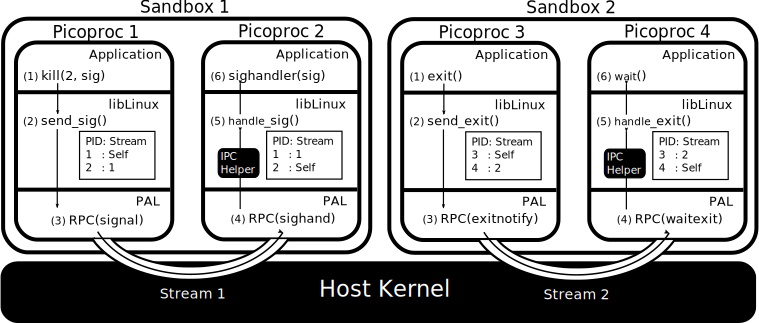
\includegraphics[width=\linewidth]{coordination.pdf}
\caption{Two pairs of \graphene{} \picoprocs{} in different sandboxes 
coordinate signaling and process ID management.
The location of each PID is tracked in {\tt libLinux}; Picoprocess 1 signals
\picoproc{} 2 by sending a signal RPC over stream 1,
and the signal is ultimately delivered using a 
library implementation of the {\tt sigaction} interface. Picoprocess 4 
waits on an {\tt exitnotify} RPC from  \picoproc{} 3 over stream 2. }
\label{fig:libos:coordination}
\end{figure}


Figure~\ref{fig:libos:coordination} illustrates two sandboxes with \picoprocs{}
collaborating to implement 
signaling and exit notification
within their own
process ID (PID) namespaces.  
Because process IDs and signals are \libos{} abstractions,
\picoprocs{} in 
each sandbox can have overlapping process IDs, and
cannot signal each other.
The host reference monitor ensures that
picoprocesses in different sandboxes cannot 
exchange RPC messages or otherwise communicate.
%If the connection between \picoprocs{} 1 and 2 is severed by subdividing the sandbox,
%the processes will become inaccessible to each other
%and each newly isolated library OS will treat the event as a process termination.



If \picoproc{} 1 (PID 1) sends a \code{SIGUSR1} to \picoproc{} 2 (PID 2), illustrated in Figure~\ref{fig:libos:coordination},
a \syscall{kill} call to \thelibos{} will check its cached mapping of PIDs to 
point-to-point streams.
If \thelibos{} cannot find a mapping, it may begin by sending a query to the leader
to find the owner of PID 2,
and then establish a coordination stream to \picoproc{} 2.
%The leader may also pass a point-to-point coordination stream handle.
Once this stream is established, \picoproc{} 1 can send a  
signal RPC to \picoproc{} 2 (PID 2).
When \picoproc{} 2 receives this RPC, 
\thelibos{} will then query its local \code{sigaction} 
structure and mark \code{SIGUSR1} as pending.
The next time \picoproc{} 2 calls \syscall{kill},
the \code{SIGUSR1} handler will be called upon return. Also in Figure~\ref{fig:libos:coordination}, \picoproc{} 4 (PID 2) waits on 
\picoproc{} 3 termination (in the same sandbox with PID 1). When \picoproc{} 3 terminates, it invokes the library implementation of exit, which issues
an \code{exitnotify} RPC to \picoproc{} 4.
%In this example, \picoprocs{} in different sandboxes have the same PID number, but this does not cause conflict as they are isolated and can only communicate with processes in the same sandbox.

%%% Using a helper thread alongside each process to asynchro-
%%% nously handle signaling
%%% is common in many \microkernel{}-based OSes such as GNU Hurd~\cite{hurd}.
%%% GNU Hurd also maintains local mappings of PIDs and RPC ports for inter-process messaging.
%%% However, PID namespace in GNU Hurd is only tracked between the parents/children, so signaling cannot be transferred between arbitrary processes.
%%% \graphene{} handles PID namespace with global consistency inside a sandbox,
%%% but requires no intensive RPCs to any centralized service.   

The signaling semantics of \thelibos{} closely match the Linux behavior, which
delivers signals upon returning from a system call
or an exception handler.
Each process and thread have \code{sigaction} structures from the Linux source 
that implement the
POSIX specification, including handler functions, as well as masking signals and
reentrant behavior.
\thelibos{} does not modify \libc{}'s signal handling code. % is unmodified on \graphene{}.
%We extend the \pal{} with ABIs for explicit upcalls on certain hardware exceptions, such
%as divide-by-zero or segmentation faults.
%Signals from other processes, such as {\tt SIGUSR1}, are generally delivered upon 
%return from a call into {\tt libLinux}; 
If an application has a signal pending for too long,
e.g., the application is in a CPU-intensive loop, {\tt libLinux} can use \palcall{ThreadInterrupt} in \thehostabi{} to interrupt the running thread. 


% Daniela Oliveira commented. old caption for coordination
%\caption{\graphene{} namespace coordination example.  
 % Two applications and {\tt libLinux} instances
 % coordinate signaling and process ID management.
 % The location of each PID is tracked in {\tt libLinux};
 % a signal message is sent over a host stream
 % using the {\tt action} message, 
 % and the signal is ultimately delivered using a 
 % library implementation of the {\tt sigaction} interface.
%}


\begin{comment}
\graphene{} internally indexes point-to-point handles using PIDs.
In order to facilitate reallocation of PIDs without global coordination, 
\graphene{}-internal PIDs also include a {\em generation number},
allowing \picoprocs{} to lazily detect reuse similar to generation numbers 
for inodes in NFS~\cite{sandberg85nfs}.
\end{comment}

\paragraph{System V IPC.} System V IPC
maps an application-specified key onto a unique identifier.
All System V IPC abstractions, including message queues and semaphores,
are then referenced by a resource ID, which is arbitrarily allocated.
Similar to process IDs, 
%In order to service IPC requests, including identifier creation, from local state,
the leader divides the namespace of resource IDs among the \picoprocs{},
so that any \picoproc{}
can allocate a resource ID from local state instead of involving the leader. %a pre-allocated range.
Unlike the resouce IDs, System V IPC keys must be centrally managed
by the leader,
since an application might autonomously assign System V IPC keys to its processes.
%The leader also dynamically allocates keys to \picoprocs{}.
Global coordination is required to ensure that the same key maps to the same resource ID;
the leader caches this information, but the owner of the resource ID 
makes the definitive decision about whether a ID mapping is still valid.
A key which does not have a valid mapping can be assigned to a resource ID by any \picoproc{} to allocate a {\em private} IPC resource.



\paragraph{System V IPC message queues.} In \graphene{}, the owner of a queue ID is responsible for 
storing the messages written to a System V IPC message queue.
To ensure the serializability and consistency of all messages, any delivery and reception of messages must go through the owner.  
In the initial implementation of \thelibos{}, sending or receiving messages remotely over a RPC stream
orders of magnitude slower than accessing a local message queue.
This observation led to two essential optimizations.  
First, sending to a remote
message queue was made asynchronous.  In the common case, the sender can simply assume 
the send succeeded, as the existence and location of the queue have already been determined.
The only risk of failure arises when another process deletes the queue.
When a queue is deleted, the owner sends a deletion notification to all other \picoprocs{}
that previously accessed the queue.
If a pending message was sent concurrently with the deletion notification 
(i.e., there is an application-level race condition), 
the message is treated as if it were sent after the deletion and thus dropped.
The second optimization migrates queue ownership from the producer to the consumer,
which must read queue contents synchronously.

%\fixmedp{bill: it is referenced in the Semaphores section, but here there isn't any talk about migrating msg queues to the most active \picoproc{}. also, the section starts with ``two essential optimizations. First \ldots'', but there isn't a second. is queue ownership migration the second?}

Because non-concurrent processes can share a message queue,
our implementation also uses a common file naming scheme to serialize message queues to disk.
If a \picoproc{} which owns a message queue exits, 
any pending messages are serialized to a file in the host,
and the receiving process may regain the ownership of the message queue later from the leader and recover the serialized messages.
%In order to prevent happens-before violations in case of failure, 
%message queues may be checkpointed more aggressively.


%\paragraph{Failure Recovery.}
%\label{sec:namespaces:failurerecovery}
%The \graphene{} coordination protocols are designed such that the leader does not store any unrecoverable information---the leader
%only caches the current name allocations.
%Because we assume that \picoprocs{} within a sandbox trust each other, 
%a new leader can simply broadcast a request to 
%recreate the current name allocations.  
%If the leader crashes, a simple leader election protocol is sufficient, e.g., picking the smallest live PID.

%\daniela{I wonder if the remainder of this section should be part of implementation details(section 5)}

\paragraph{System V IPC semaphores.} System V IPC semaphores 
follow a similar pattern to message queues.
Each semaphore is owned by a \picoproc{};
a semaphore can be directly accessed by its owner as a local state,
whereas other \picoprocs{} all have to access the semaphore through the owner over RPC.
Since a semaphore shares the same performance pattern as a message queue,
\thelibos{} applies the same optimization
of migrating the ownership of a semaphore
%, where ownership of a given semaphore is migrated
to the \picoproc{} that most frequently acquires the semaphore.
%If the owner of a semaphore exits, \graphene{} transfers ownership to the leader.  rather than serialize the semaphore to disk.
Another optimization of message queues, by making the updates asynchronous,
does not apply to semaphores,
because a participating \picoproc{} cannot proceed before successfully acquiring the semaphore. 
Most of the overhead in the Apache benchmark (see Section~\ref{sec:eval:graphene}) is attributable to semaphore overheads.
%and, in ongoing work, we will likely optimize this by 
%either expanding the host ABI to share synchronization primitives within a sandbox,
%using shared memory to reduce semaphore latency.

\paragraph{Shared file descriptors.}
The seek pointer of each file descriptor is implemented as a \libos{} abstraction;
when reading or writing to a host file,
\thehostabi{} always obtains an absolute pointer from the beginning of the file.
Although most applications
do not share the seek pointer of an inherited file descriptor among processes,
the {\tt clone} system call
can can be called with the {\tt CLONE\_FILES} flag
and create a process
which shares the whole file descriptor table with its parent.
%The default Linux behavior is that children copy the open handles and file seek cursors,
%but subsequent cursor movements are not shared between parent and child.
%Shared file descriptor table can be requested by passing the {\tt CLONE\_FILES} flag to the {\tt clone} system call.
%Any new file descriptor opened in a shared table will be visible by every process cloned in this way, as well as subsequent cursor update.
%None of our target applications have required a shared seek cursor, and it is not currently implemented,
%but would be a straightforward extension to current RPC mechanisms.
%We expect that the current RPC mechanisms could easily be extended to synchronize a seek pointer among \picoprocs{}.
To share a file descriptor table among \picoprocs{},
one of \picoprocs{} (usually the oldest one)
must be the leader of the file descriptor table to manage all mappings
from file descriptors to the child \picoproc{} who owns the state of the file descriptors including the seek pointers.
Every updates to a seek pointer must goes through the owner of the file descriptor (not the leader).
The migration-based optimization for System V IPC message queues and semaphores is also effective for optimizing the performance of shared file descriptors. 

\paragraph{Shared file system states.}
A chroot file system in \thelibos{}
is restricted by \thehostabi{} to externalize any file system states.
Other shared file system states are implemented as \libos{} abstractions, and have to be coordinated among \picoprocs{}.
For example, a POSIX file system can contain special files such as a FIFO (first-in-first-out); a path bound to a UNIX domain socket;
a symbolic link; or a file system lock.
Implementation of these special files cannot
completely depend on \thehostabi{},
since the abstractions of \thehostabi{} contains only regular files and directories.

%Coordinating these states can be cause significant slowdown on regular file system operations, so we simply export the state in regular files on the host,
% and atomically update them by renaming.

A simple approach to coordinating file system states is to share a ``dummy'' host file.
For example,  \thelibos{} can store the target of a symbolic link
in a regular file on the chroot file system.
For a FIFO, a bounded UNIX domain socket, or a file system lock,
\thelibos{} can store a mapping to the corresponding RPC stream, or to the \picoproc{} which owns the abstraction.
By using the host file system as a less efficient but permanent coordination medium,
\thelibos{} can extend the coordination framework for sharing file system states.



\paragraph{Shared memory.} The \graphene{} architecture 
does not currently permit shared memory among \picoprocs{}.
This thesis expects that an extra \hostapi{} and the existing support for System V IPC coordination would be sufficient to implement this,
with the caveat that the host must be able to handle sandbox disconnection gracefully, perhaps converting the pages to copy-on-write.
Thus far \graphene{} have avoided the use of shared memory in \thelibos{},
both to maximize flexibility in placement of \picoprocs{}, potentially on an unconventional host (e.g., Intel SGX) or different physical machines.
and to keep all coordination requests explicit.
Shared memory may also be useful to reduce latency for RPC messaging among \picoprocs{} when 
all \picoprocs{} are on the same host.


%in \graphene{} are implemented by a simple producer-consumer model.
%%% Without blocking, the latency of an inter-process semaphore operation equals to a round-trip of RPC messages.
%%% We observed that IPC semaphores can benefit from the same optimization
%%% used by message queues,
%%% based on asynchronous sending.
%%% However, when non-concurrent processes share a semaphore, it does not worth serializing the semaphore state to disk.
%%% When the owner of a semaphore exits,
%%% the semaphore state will be migrated to the leader,
%%% if it has a non-zero counter.
%%% IPC semaphores are intensively used in Apache web servers with a multi-process model. 

 


\paragraph{Failure and disconnection tolerance.}  
\thelibos{} must tolerate disconnection between collaborating \picoprocs{},
either because of crashes or blocked RPC streams.  In general, \thelibos{} makes 
these disconnections isomorphic to a reasonable application behavior,
although there may be some edge cases that cannot be made completely transparent to the application.

In the absence of crash recovery, placing shared state in a given \picoproc{} introduces the risk that an errant 
application will corrupt shared \libos{} state.  The \microkernel{} approach of 
moving all shared state into a separate server process is more resilient to this problem.
Anecdotally, \thelibos{}'s performance optimization of migrating ownership to the process that 
most heavily uses a given shared abstraction also improves the likelihood that only the corrupted
process will be affected.  
Making each \thelibos{} instance resilient to arbitrary memory corruption of any \picoproc{} is left for future work.


\paragraph{Leader recovery.}
\thelibos{} provides a leadership recovery mechanism when a leader failure is detected.
A non-leader \picoproc{} can detect the failure of a leader by either observing the shutdown of RPC streams or timing out on waiting for responses. 
Once the \picoproc{} detects leader failure, \thelibos{} sends out a message on the broadcast stream to volunteer for claiming the leadership.
After a few rounds of competition, the winning \picoproc{} becomes the new leader and recover the namespace state by reading a namespace snapshot stored before the crash of the former leader
or recollecting from other \picoprocs{} in the same sandbox.

%After a \picoproc{} being elected as the leader,
%the leader state,
%including all the allocated IDs and the RPC stream addresses,
%must be recovered. 
%Recollecting the leader state from all the \picoprocs{} is possible
%but can be inefficient,
%given the new leader may not have knowledge about every \picoproc{}.
%To simplify the implementation,
%we make the leaders of a namespace periodically serialize their states to disk for later recovery.

When a \picoproc{} is moved to a new sandbox, \thelibos{} will naturally detect the failure of leader because of blocked RPC. % streams are closed by the reference monitor.
The sandboxed \picoproc{} will be the only candidate for leadership because the host has replaced the broadcast stream;
as a result, the sandboxed \picoproc{} seamlessly transitions to new namespaces isolated from the previous sandbox.

%Once it starts the leadership recovery, it will automatically win because no other \picoproc{} is sharing the broadcast stream. The procedure can be skipped by informing the sandboxed \picoproc{} before detaching.

\subsection{Lessons learned}
\label{sec:libos:namespaces:lessons}

The current coordination design is the product of several iterations, which began 
with a fairly simple RPC-based implementation. %, and was then refined based on profiling.
This subsection summarizes the design principles that have emerged from this process.
%We present high-level facets of the design along with the insight
%behind the decision.  The next subsections synthesize these aspects 
%with specific examples of signaling and message queues.

\paragraph{Service requests from local state whenever possible.}
Sending RPC messages over Linux pipes is expensive;
this is unsurprising, given the long history of 
work on reducing IPC overhead in microkernels~\cite{liedtke93sosp,chen93memory}.  
We expect that \graphene{} performance could be improved on a 
\microkernel{} with
a more optimized IPC substrate, such as L4~\cite{liedtke95sosp,klein09sel4,elphinstone13microkernels};
we take a complementary approach of avoiding IPC if possible.
%but this is beyond the scope of our work, and we want \graphene{} to perform well on any 
%host OS.

An example of this principle is migrating message queues to the ``consumer'' when a 
clear producer/consumer pattern is detected, or migrating semaphores to the most frequent requester.
In these situations, synchronous RPC requests can be replaced with local function calls, improving
performance substantially.  For instance, migrating ownership of message queues 
reduced overhead for message receive by a factor of $10\times$.

\paragraph{Lazy discovery and caching improve performance.}  
No library OS keeps a complete replica of all distributed state,
avoiding substantial overheads to pass messages replicating irrelevant state.
Instead, \graphene{} incurs the overhead of discovering the owner of a name
on the first use, and amortizes this cost over subsequent uses.
Part of this overhead is potentially establishing a point-to-point stream,
which can then be cached for subsequent use.
For instance, the first time a process sends a signal, the helper thread 
must figure out whether the process id exists, to which \picoproc{} it maps,
and establish a point-to-point stream to the \picoproc{}.
If they exchange a second signal, the mapping is cached and reused, amortizing this 
setup cost.  For instance, the first signal a process sends to a new processes
takes \roughly{}2ms, but subsequent signals take only \roughly{}55 \us{}.

\paragraph{Batched allocation of names minimizes leader workload.}
In order to keep the leader off of the critical path of operations like {\tt fork}, 
the leader typically allocates larger blocks of names, such as process IDs or System V queue IDs.
In the case of \syscall{fork}, if a \picoproc{} creates a child, it will request a batch of 
PIDs from the leader (50 by default).  Subsequent child PID allocations will be made from the same 
batch without consulting the leader.
Collaborating processes also cache the owner of a range of PIDs, avoiding 
leader queries for adjacent queries.

%% dp: Sad to see this go, but it is sort of subsumed by the other discussion
\paragraph{The coordination within a sandbox is often pairwise.}
\graphene{} optimizes the common case of pairwise coordination,
by authorizing one side of the coordination to dictate the abstraction state,
but also allows
more than two processes to share an abstraction.
Based on this insight, 
we observe that {\em not all shared state need be replicated by all \picoprocs{}}.
Instead, we adopt a design where one \picoproc{} is authoritative for a given name (e.g., a process ID or a System V queue ID).
For instance, all possible thread IDs are divided among the collaborating \picoprocs{},
and the authoritative \picoproc{} either responds to RPC requests for this thread ID (e.g., a signal)
or indicates that the thread does not exist.
This trade does make commands like ``\code{ps}'' slower, 
but optimizes more common patterns, such as waiting for a child to exit.

\paragraph{Make RPCs asynchronous whenever possible.} 
For operations that must write to state in another \picoproc{}, 
the \graphene{} design strives to cache enough information in the sender 
to evaluate whether the operation will succeed, thereby obviating the 
need to block on the response.  This principle is applied to lower the overheads
of sending messages to a remote queue.


%this is a mapping to a thread within a specific \picoproc{}; for a message queue key,
%the mapping might be empty if the queue does not exist, or it may point to the \picoproc{} storing the pending messages.
%% The general problem underlying each of these coordination APIs is 
%% {\bf namespace management}.  In other words, coordinating \picoprocs{} need a consistent mapping
%% of names, such as a thread ID or System V message queue ID, to the authoritative \picoproc{} for that abstraction, if one exists.


\paragraph{Summary.}
The current \graphene{} design minimizes the use of RPC,
avoiding heavy communication overheads in the common case.
This design also allows for substantial flexibility to dynamically moving processes out of
a sandbox.  Finally, applications do not need to select different 
library OSes {\em a priori} based on whether they are multi-process or single-process---\graphene{}
automatically uses optimal single-process code until otherwise required.

%\section{Minimizing the TCB with the Non-Partitioned Model}

%\subsection{Reducing the TCB in \libos{}}
%\subsection{Partitioning the TCB in Multi-Process Applications}





\makeatletter
\def\input@path{{}}
\makeatother
\graphicspath{{}}
\chapter{The Host ABI}
\label{chap:abi}

\makeatletter
\def\input@path{{abi/}}
\makeatother
\graphicspath{{abi/figures/}}

\lstnewenvironment{paldef}{
  \noindent\minipage{\linewidth}\medskip
  \lstset{
    basicstyle=\ttfamily\footnotesize, %
    frame=single, %
    rulecolor=\color{gray!30}, %
    backgroundcolor=\color{gray!30}, %
    showspaces=false, %
    showstringspaces=false, %
    lineskip=2pt, % 
    aboveskip=0.25\baselineskip, %
    belowskip=1.00\baselineskip, %
    framesep=10pt, %
    framexleftmargin=5pt, %
    framexrightmargin=5pt, %
    xleftmargin=.5in,
    xrightmargin=5pt,
    breaklines, % 
    breakatwhitespace, %
    breakindent=0pt %
  }
}{ %
  \endminipage
}

\declarecommand{\palkeyword}[1]{\setlength{\fboxsep}{0pt}\colorbox{gray!30}{\lstinline[basicstyle=\ttfamily\small]{#1}}} 
\declarecommand{\palcall}[1]{\palkeyword{#1()}} 

This chapter describes the formal definition of the \graphene{} host ABI.

\section{Basic Definitions}

The \graphene{} host ABI defines a set of {\em functions}, similar to the API of UNIX or POSIX.
The functions are directly called by the library OS, along with the arguments given either in the registers or on the stack.
A host-specific \graphene{} loader is responsible for resolving the linking, from the library OS to the host ABI.
\subsection{Stream I/O}
\label{sec:abi:streams}



\issuedone{1.2.a}{discuss resource management at host level (I/O)}
I/O is part of the foundation
of an OS, to allow an application to interact with
other machines, users, applications, or system software.
An OS typically supports three types of I/O:
%An application requires interaction with the world during its execution, using I/O devices.
%I/O is a common feature of almost every OSes.
%The typical I/O needed in an application
%can be catagorized into three types:
{\bf storage}, for externalizing data to a permanent store;
{\bf network}, for exchanging data with another machine over internet;
and {\bf RPC} (remote procedure call),
for connecting concurrent applications or processes.
An OS must contain features for all three types of I/O abstractions,
and manages the resources on I/O devices, such as hard drives and NICs (network interface controllers).
Therefore, unless an I/O device is virtualized and dedicated to
an application or a guest,
a host OS must take a major role in I/O management;
for the least, a host OS has to share the resources among multiple applications or guests,
and contain the drivers to interface with the I/O devices.




%externalizing data to outside of the machines (i.e., networking);
% (i.e., storage);
%and  (i.e., remote-procedure call).
%A modern OS may define several abstractions
%for each types of I/O; for example, a file in Linux can be read using several system calls,
%including \syscall{read}, \syscall{pread}, and \syscall{readv};
%RPC in Linux is based on multiple inter-process abstractions,
%including pipes, UNIX sockets, and signals.




\fixmedp{Perhaps you want to start with defining a single byte stream abstraction? And then talk about how different URIs leads to different subclasses?}
The basic I/O abstraction in the host ABI
is a simple byte stream.
A byte stream allows sending or receiving information over an I/O device
as a continuous byte sequence.
According the type of I/O, a byte stream is restructured as the I/O device demands;
for example, on a storage device,
a byte stream is logically stored as a sequential file,
but physically divided into blocks;
on a NIC, a byte stream is transfered as packets, and identified by IP address and port number bound to a network socket;
a RPC stream can be simply a FIFO (first-in-first-out),
which applications or processes use to pass messages.
The host ABI for I/O is similar to the API of a UNIX-style OS,
which treats ``everything as a file descriptor''
and allows utilizing different types of I/O devices through the same file system APIs, including \syscall{read} and \syscall{write}.
Managing I/O as byte streams simplifies the development of both the library OS and PALs.
%The host ABI includes \hostapis{} for single-flavored, stream-type I/O, similar to the API of a UNIX-style OS.
%In general, a UNIX-style OS
%follows the design where ,
%meaning that each I/O abstraction is encapsulated by the file system APIs, such as \syscall{read} and \syscall{write}, to send and receive data on a file, a network socket, or a FIFO (first-in-first-out).
%but categorizes into three types:
%{\bf network connections}, {\bf regular files}, and {\bf RPC streams}.


The host ABI identifies I/O streams by URIs (unified resource identifier).
%These I/O streams
%are created or connected using a URI (unified resource identifier),
A URI is a unique name which describes 
both the subclass of an I/O stream, and the information for locating or identifying an I/O stream on an I/O device or inside the host OS.
The subclass of an I/O stream is identified by the URI prefix,
a keyword that represents different types of I/O: ``\palkeyword{file:}'' for regular files; ``\palkeyword{tcp:}'' and ``\palkeyword{udp:}'' for network connections; and ``\code{pipe:}'' for RPC streams.
The rest of the URI represents an identifier of the I/O stream:
for example, a file can be identified by a path located in a hierachical file system;
a network connection can be identified by the socket address.
The URIs standardize the way of identifying I/O resources inside various host OSes.


%According to the prefix of URI,
%the PAL can create either a synchronous I/O stream (e.g., a file or a connected socket)
%or named I/O server (e.g., a listening TCP socket).
%Modern OSes contain several out-of-band or asynchronous I/O abstractions, to improve the latency or CPU idle time
%when polling I/O streams.
%Although using out-of-band or asynchronous I/O is beneficial for application performance,
%providing these I/O features can be challenging for a host.
%Therefore, in \graphene{}, the host ABI restricts I/O abstractions to only synchronous stream I/O.


\fixmedp{Define these semantics without a reference to POSIX, so that the document is self-contained.}
The \hostapis{} defined in the host ABI for I/O are as follows:
%The host ABI for stream I/O presents a simplified, {\b POSIX file system}.
%A POSIX file system
%encapsulates I/O abstractions,
%including files, sockets, pipes, and even character devices,
%in the file system API.
%The host ABI contains several functions
%which resemble the POSIX API:
\palcall{StreamOpen} creates or opens an I/O stream;
\palcall{StreamRead} and \palcall{StreamWrite}
send and receive data over an opened I/O stream;
%are similar to \syscall{open}, \syscall{read}, and \syscall{write} in behavior, with a simplified, explicit semantic;
\palcall{StreamMap} maps %a is equivalent to \syscall{mmap} with a \code{MAP\_FILE} flag, mapping
a regular file to the application's memory; %, for reading or writing data.
\palcall{StreamAttrQuery} and \palcall{StreamAttrQuerybyHandle}
retrieves the file metadata and I/O attributes;
%as \syscall{stat} and \syscall{fstat} do;
%The POSIX-style functions simplify the porting of the host ABI
%on hosts with a similar specification.
\palcall{StreamWaitForClient} blocks and creates an I/O stream for incoming network or RPC connection;
\palcall{StreamSetLength} truncates a regular file;
\palcall{StreamFlush} clears the I/O buffer inside the host OS.
The following sections will discuss these \hostapis{} in details.





\subsubsection*{Opening or creating an I/O stream}




\begin{paldef}
HANDLE StreamOpen (const char *stream_uri,
                   u16 access_flags, u16 share_flags,
                   u16 create_flags, u16 options);
\end{paldef}



\palcall{StreamOpen} opens an I/O stream, % for future operations,
according to a URI given by \palkeyword{stream_uri} as a string argument. % to identifies resources associated with the I/O stream. 
The specification of 
\palcall{StreamOpen} includes interpreting the URI prefixes and syntaxes of \palkeyword{stream_uri},
and allocating the associated resources in the host OS and on the I/O devices.
\fixmedp{The term ``Opaque pointer'' is useful here}
If \palcall{StreamOpen} succeeds, it returns a {\bf stream handle}.
A stream handle is stored by the guest as an identifier to the opened I/O stream.
A stream handle is an opauqe pointer, which means the guest should only reference it as an identifier, and never try to interpret the content.
On the other hand, if \palcall{StreamOpen} fails (e.g., invalid arguments or permission denied), it returns a null pointer with the failure reason delivered with an exception.
% A stream handle is similar to a file descriptor in the POSIX API,
%but defined as a pointer to a data structure containing the stream information.
%The internal structure of a stream handle is up to the I/O stream type and the implementation of each PAL;
%a library OS is supposed to reference a stream handle
%only as an identifier.


\fixmedp{Need a listing of all the values of flags}
Other arguments of \palcall{StreamOpen} specify the options for opening an I/O stream:

\begin{compactitem}

\item
\palkeyword{access_flags} specifies the access mode of the I/O stream, which can be either \palkeyword{RDONLY} (read-only), \palkeyword{WRONLY} (write-only), \palkeyword{APPEND} (append-only), and \palkeyword{RDWR} (readable-writable).
The first three access modes are only available
for regular files; if the opened stream is a network or RPC stream, the access mode is always \palkeyword{RDWR}.
The access modes specify the basic access permissions that an application can request when opening a file.
The access permissions are validated by the host OS, based on user configurations.
For example, a file configured as append-only for the running application can only be opened in the \palkeyword{APPEND} mode.

\item
\palkeyword{share_flags} specifies the permissions for sharing a regular file (ignored for other types of  I/O streams)
with other applications, either in \graphene{} or in the host OS.
\palkeyword{share_flags} can be a combination of six different values:
\palkeyword{OWNER_R}, \palkeyword{OWNER_W}, and \palkeyword{OWNER_X}
represent the permissions to be read, writed, and executed by the creater of the file;
\palkeyword{OTHER_R}, \palkeyword{OTHER_W}, and \palkeyword{OTHER_X}
represent the permissions to be read, writed, and executed by everyone else.
The permissions are externalized to the host file system; access modes given in future execution are validated against the permissions.

\item
\palkeyword{create_flags} specifies whether to create a regular file,
when it does not exist in the host file system.
If \palkeyword{create_flags} is given as \palkeyword{TRY_CREATE},
it creates the file no matter if the file exists.
If \palkeyword{create_flags} is given as \palkeyword{ALWAYS_CREATE},
it fails if the file already exists.

\item
\palkeyword{options} specifies a set of miscellaneous options to configure the opened I/O stream.
Currently \palcall{StreamOpen} only accepts one option: \palkeyword{NONBLOCK} specifies that the I/O stream will never block whenever the guest attempts to read or write data.
The nonblocking I/O option is necessary for performing asynchronous I/O in the guest, to overlap the blocking time of multiple streams by polling (using \palcall{ObjectsWaitAny}).

\end{compactitem}


%includes different syntaxes for interpreting the URI and the rest of arguments,
%and different behaviors for creating or opening an I/O stream,
%according to the URI prefixes.
%uses a URI (uniform resource identifier), for specifying the I/O stream.
%An URI identifies both the type of I/O and the distination or location of the I/O stream.
%The type of a I/O stream is determined by URI prefix.
According to the consecutive operations, \palcall{StreamOpen}
returns two types of handles: One type represents a simple byte stream;
the other type is a server handle, which can wait on remote clients to initiate handshakes
for creating a byte-stream connection.
A server handle can be bound as a network server or a RPC server.
Because a server handle is not a byte stream, it cannot be directly read or written,
but can be given to \palcall{ServerWaitForClient} to block and receive a client connection.
The host ABI includes the abstraction of creating server handles
because receiving client connections requires control at the TCP/IP layer
and allocating host resources,
which cannot be implemented in the guest unless
the network stack is virtualized.




\palcall{StreamOpen} accepts the following URI prefixes and syntaxes for creating a byte stream or a server handle:


\begin{compactitem}

\item \palkeyword{file:[path]} creates or opens a regular file on the host file system.
The opened file is located by a path---either an absolute path from the root of the host file system, 
or a relative path.
\fixmedp{Mention CWD is relative to where the app is launched from. It may also be worth noting that this is included for convenience, but there are some security risks to using relative paths.}
A relative path is located from the initial directory where the application is launched,
and will never change afterward.
\palcall{StreamOpen} accepts relative paths for the convenience of locating application files packaged and shipped together.
Note that there could be security concerns
that a relative path may collide with another absolute path, or be ambiguous if the path starts with a ``dot-dot'' (i.e., walking back a directory).
Fortunately, both cases can be checked by the guest, as long as
the initial directory is specified by the host.
%based on user configurations.

\item \palkeyword{tcp:[address]:[port]} or \palkeyword{udp:[address]:[port]} creates a TCP or UDP connection to a remote server,
based on the IPv4 or IPv6 address and port number of the remote end.
One a connection is created,
it will exists until it is torn down by both sides.

\item \palkeyword{tcp.srv:[address]:[port]} or \palkeyword{udp.srv:[address]:[port]} create a TCP or UDP server handle which can receive remote client connections.
A TCP or UDP server is bound on a IPv4 or IPv6 address and an idle port number.
If the specified port number is smaller than 1024,
it may require additional privilege from the host OS.

\item \palkeyword{pipe.srv:[name]} or \palkeyword{pipe:[name]} create a named RPC server or a connection to a RPC server.
The name of a RPC server is an arbitrary, unique string.
An RPC stream is an efficient way for passing messages between applications or processes
running on the same host,
compare with using a network stream locally.
An RPC stream is supposed to be low-latency, and can scale up to significantly
more concurrent connections
than the limitation on network streams.

%The stream can be either a server which awaits incoming connection from other processes,
%or a client to an existing server.

\end{compactitem}



%Besides the abstraction,
%\palcall{StreamOpen}
%also inherits similar definitions of function arguments,
%including \palkeyword{access_flags}, \palkeyword{share_flags}, \palkeyword{create_flags}, and \palkeyword{options},
%from the POSIX-style \syscall{open}.
%%also inherit similar meanings from the options of \syscall{open}.
%These arguments specify the access type, file permission, creation mode, and other miscellaneous options of the I/O streams:
%for example, the access type can be specified as readable or writable,
%and the creation mode can be either explicit or implicit.
%An important concern is the choice of file permission (specified by \palkeyword{share_flags}), since the host ABI does not expose user credentials
%from the host.
%Setting the file permission in the host
%is mostly a usability feature: 
%an application can run more smoothly if some file permissions are externalized.
%For example, a compilor can create an executable with the execution permission, so that the consecutive building script can run the executable.
%The host ABI also externalizes the file permission
%which specifies specify whether a file can be shared with other applications.


\palcall{StreamOpen} defines the scope of enforcing and configuring security isolation in the hosts.
%URIs for \palcall{StreamOpen} represent three types of 
The host ABI restricts the sharing of host resources
to type types of simple I/O streams (i.e., file, network, and RPC). 
Other host resources, such as threads and memory,
are local to each process, and thus can be isolated by dedicating the host resources.
%Restricting the shareable host resource to I/O streams simplifies
%the enforcement of security policies in the hosts.
Therefore, in the host ABI, \palcall{StreamOpen} is the only \hostapi{}
which requires permission checks in the hosts.
Moreover, a user can configure the policies of sharing I/O streams by
whitelisting the URIs that are permitted for an application.





\subsubsection*{Reading or writing an I/O stream}



\begin{paldef}
u64 StreamRead  (HANDLE stream_handle, u64 offset,
                 u64 size, void *buffer);
u64 StreamWrite (HANDLE stream_handle, u64 offset,
                 u64 size, const void *buffer);
\end{paldef}                   
              
\palcall{StreamRead} and \palcall{StreamWrite} synchronously
read and write data over an opened I/O stream.
Both \hostapis{} receive four arguments: a \palkeyword{stream_handle} for referencing the target I/O stream;
\palkeyword{offset} from the beginning of a regular file
(ignored if the stream is a network or RPC stream);
\palkeyword{size} for specifying how many bytes are expected to be read or written;
and finally, a \palkeyword{buffer} for storing the read or written data.
At success, the \hostapis{} return the number of bytes
actually being read or written.


     




%The host ABI features include synchronously reading and writing data over an I/O stream.
%The behavior of \palcall{StreamRead} and \palcall{StreamWrite} is slightly different between a file stream and other type of stream:
%when reading or writing a file stream, \palcall{StreamRead} and \palcall{StreamWrite} accesses the file at a specific offset from the beginning of the file;
%otherwise, when accessing a network or RPC stream,
%the argument \palkeyword{offset} is ignored, and thus the ABI works similar to \syscall{read} and \syscall{write}.



\palcall{StreamRead} and \palcall{StreamWrite} avoid the semantics of sequential file access
to skip the migration of stream handles.
A regular file opened by \palcall{StreamOpen} (not in the append-only mode)
can only be read or written at an absolute offset
from the beginning of the file.
The random file access prevents the host OSes to track the offset
as an internal state,
and allows a migrated guest to reopen the I/O stream on another host
without migrating the host OS states.
Because all the host OS states associated with an I/O stream is only meaningful to the host,
and can be receated anytime,
the I/O stream appears to be {\em stateless} to the guest.



%The design is to keep the stream handle stateless inside the PAL,
%for cleanly migrating a library OS.
%Since the library OS is responsible of maintaining the offset of a file descriptor,
%a library OS instance can be easily detach from a PAL,
%by simply ``invalidating'' a stream handle;
%the library OS should be able to always reopen the stream after migration,
%or after a failure of accessing a stream handle,
%to recover the state of an I/O stream.



The host ABI does not includes asynchronous I/O semantics, or peeking into network or RPC buffers inside the host OS.
%Another challenge in the library OS, regarding I/O streams,
%is to support asynchronously I/O, or peeping data received over a network or RPC stream.
%This design decision is made to keep the host ABI simple.
Asynchronous I/O and peeking the buffers are both
common OS features that an application may depend on.
Although the features are not included in the host ABI,
the guest (i.e., the \libos{}) is supposed to emulate these features using the synchronous \palcall{StreamRead} and \palcall{StreamWrite},
combined with other \hostapis{} (e.g., \palcall{ObjectsWaitAny})
to prevent blocking on an I/O stream.
The guest can also allocate its own buffer to store data prematurely received from an I/O stream,
to serve the buffer peeking feature.
More details of these features are discussed in Chapter~\ref{chap:libos}.

%To implement the full Linux I/O features,
%the library OS must emulate asynchronous I/O,
%using the synchronous
%\palcall{StreamRead} and \palcall{StreamWrite}.
%The emulation requires opening the I/O stream in a non-blocking mode,
%and polling the stream handle before reading or writing data.
%The library OS can also buffer the data being read or written over a stream,
%as long as the buffered state is coordinated over every processes
%which share the same stream.


\paragraph{Alternative.}
An alternative strategy is to define a host ABI with asynchronous I/O semantics.
An asynchronous read or write
does not return a result immediately; instead, it creates an event handle
which can be polled arbitrarily.
An ABI that asynchronously reads and writes an I/O stream
potentially has more predictable semantics,
because the guest can explicitly tell which \hostapis{} will be blocking.
This strategy
is taken by Bascule~\cite{baumann13bascule}.
\graphene{} chooses synchronous I/O over asynchronous I/O in the current host ABI,
because synchronous I/O is a more common feature in host OSes.


 


%Defining  \hostapis{} for asynchronous read and write
%may potentially sacrifice portability, \fixme{cites some host that doesn't have async IO}
%since asynchronous I/O is less common seen in OSes.
%However, 
%can potentially be a more flexible option for emulating other I/O features in the guest.
%For example, the guest can emulate a synchronous read by polling a stream followed by asynchronously reading it.



%An asynchronous I/O ABI can be potentially
%more flexible for implementing the library OS features,
%as it can emulate both synchronous and asynchronous behaviors
%without buffering.
%The only reason that we choose synchronous over asynchronous I/O
%in the host ABI is to reduce the porting effort,
%especially for a host which lacks
%asynchronous I/O features.



\subsubsection*{Mapping a file to memory}
                   
\begin{paldef}            
u64 StreamMap (HANDLE stream_handle, u64 expect_addr,
               u16 protect_flags, u64 offset, u64 size);
\end{paldef}


\palcall{StreamMap} maps a file stream to an address in memory, for reading and writing data, or executing code stored in a binary file.
\palcall{StreamMap} creates a memory region
as either a copy of the file,
or a pass-through mapping which shares file updates with other processes.
When calling \palcall{StreamMap},
the guest specifies an expected address in memory for mapping the file, or a null address (i.e., zero) for mapping at a random address decided by the host.
\palkeyword{expect_addr}, \palkeyword{offset}, and \palkeyword{size} have to be aligned
with the allocation granularity of the hosts (more discussion in Section~\ref{sec:abi:memory}).
\palkeyword{protect_flags} specifies the protection mode
of the memory mapping, as a combination of \palkeyword{READ} (readable), \palkeyword{WRITE} (writable), \palkeyword{EXEC} (executable), and \palkeyword{WRITE_COPY} (writable local copy).
At success, \palcall{StreamMap} returns the starting address of the mapped area; otherwise, a null address is returned.




The host ABI includes \palcall{StreamMap} for two reasons. First, memory-mapped I/O is suitable for certain file access patterns of applications, and cannot be fully emulated by the guest using \palcall{StreamRead} and \palcall{StreamWrite}.
An application often chooses memory-mapped I/O for
avoiding the overhead of memory copy and context switch, %, especially when the application contains
for frequent, small, random file reads and writes.
Second, memory-mapped I/O is asynchronous by nature.
The data written to a file-backed memory mapping can be lazily flushed out to the storage;
the same feature is difficult to emulate in the guest
%due to lack of ability to efficiently determine which pages are recently updated,
% and thus should be synchronized with the storage.
without an efficient way of marking recently-updated pages (page table dirty bits can only be accessed in host OSes).
%without access to dirty bits in the page table.




%However, the challenge to implementing this behavior
%is to externalize the latest file state
%written by the application,
%on a host which disallows file-backed memory.
%For example, in a SGX enclave, all memory will have to be private memory,
%to be individually encrypted by the CPU.
%For a host which doesn't support pass-through file mappings,
%\palcall{StreamMap}
%can only guarantee writing out
%the latest file state to the disk when the memory is unmapped, using \palcall{VirtMemFree}.


\fixmedp{there should be an explicit semantics about when the mapping is visible back to the host, like on a sync, with the option to flush earlier}
Although \palcall{StreamMap} allows multiple processes to map the same file into memory, it does not guarantee the data to be coherently shared across processes.
Because memory-mapped I/O is asynchronous,
the data written in the memory is only guaranteed to be flushed to the storage
when the memory mapping is unmapped.
Also, the host ABI drops the assumption of memory sharing, especially for an isolated environment like SGX.
It is optional for the host to flush earlier,
or to coherently share the memory across multiple processes.













\subsubsection*{Listening on a server}


\begin{paldef}
HANDLE ServerWaitforClient (HANDLE server_handle);
\end{paldef} 


\palcall{ServerWaitforClient} waits on a network or RPC server handle, %created with a URI that starts with \palkeyword{tcp.srv:}, \palkeyword{udp.srv:}, or \palkeyword{pipe.srv:},
to receive an incoming client connection.
%Besides the I/O streams which can be directly read or written,
%the host ABI also supports creation
%of I/O stream server, which can be
%connected from another process (to a RPC stream server), or another host (to a network server), as a client of the server.
A network or RPC server handle cannot be accessed by \palcall{StreamWrite} or \palcall{StreamRead};
instead, the host OS listens on the server handle,
and negotiates the handshakes for incoming connections.
Once a connection is fully established,
the host OS returns a client stream handle, which can be read or written as a simple byte stream.
Before any connection arrives, \palcall{ServerWaitforClient} blocks eternally.
if a connection arrives before the guest calls \palcall{ServerWaitforClient},
the host can optionally buffer the connection in a limited backlog; the maximal size of server backlogs is up to the user configurations. The host will drop incoming connections when the backlog is full.




%I/O stream server has to block until a client
%connects the server, using \palcall{StreamWaitForClient}.
%\palcall{StreamWaitForClient} will return a stream handle, which represents a connection with the client.
%Other implementation
%is up to the host: for example,
%the host may decide a maximal number of incoming connections to buffer.









\subsubsection*{File and stream attributes}

%The host ABI features also include retrieving the metadata of an I/O stream.
%The retrieval of metadata is not limited to files,
%but also network sockets and RPC streams. %, to query the information regarding the streams.
%An example of metadata is the address of a network stream;
%when an unbound network stream is created,
%the host will randomly bind the stream to a local, temporary port, for identifying the connection at the IP (internet protocol) level;
%the POSIX API
%reveals the local port number
%to the applications,
%using \syscall{getsockname}.
%Other stream metadata required by Linux or POSIX functionality
%includes the total bytes written over an I/O stream, and the permission to sharing an I/O stream with other applications.
%The host ABI includes two functions for querying stream metadata:

\begin{paldef}
bool StreamAttrQuerybyHandle (HANDLE stream_handle,
                              STREAM_ATTRS *attrs);
bool StreamAttrQuery (const char *stream_uri,
                      STREAM_ATTRS *attrs);

\end{paldef}

Both \palcall{StreamAttrQuerybyHandle} and \palcall{StreamAttrQuery} query the attributes of an I/O stream, and return the attributes in a \palkeyword{STREAM_ATTRS} data structure.
The only difference is that \palcall{StreamAttrQuerybyHandle} queries an opened stream handle,
whereas \palcall{StreamAttrQuery} queries a URI without opening the I/O stream.
\palcall{StreamAttrQuery} is convenient for querying stream attributes when the guest is not planning to access the data of an I/O stream.
%Because \palcall{StreamOpen} involves more operations in the host OS,
%\palcall{StreamAttrQuery} can quickly retrieve the attributes without actually opening the stream.
Both \hostapis{} return true or false for whether the stream attributes are retrieved successfully.



%Both functions fill out a data structure given by the library OS,
%with metadata regarding an I/O stream
%identified by either a stream handle or a URI.
%Keeping both functions can be convenient for the library OS to query a file without creating a stream handle;
%however, we can always consolidate the host ABI
%with only \palcall{StreamAttrQuerybyHandle},
%because \palcall{StreamAttrQuery} can be replaced by \palcall{StreamAttrQuerybyHandle}
%after \palcall{StreamOpen}.




\begin{paldef}
typedef struct {
    u16 stream_type, access_flags, share_flags, options;
    u64 stream_size;
    u64 recvbuf, recvtimeout;
    u64 sendbuf, sendtimeout;
    u64 lingertimeout;
    u16 network_options;
} STREAM_ATTRS;
\end{paldef}


The \palcall{STREAM_ATTRS} data structure consists of multiple fields specifying the attributes assigned to an I/O stream since creation.
\palkeyword{stream_type} specifies the type of I/O stream that the handle references to.
\palkeyword{access_flags}, \palkeyword{share_flags}, and \palkeyword{options} are the same attributes assigned to an I/O stream when the stream is created by \palcall{StreamOpen}.
\palkeyword{stream_size} has different meanings for files and network/RPC streams:
if the handle is a file, \palkeyword{stream_size} specifies the total size of the file;
if the handle is a network or RPC stream, \palkeyword{stream_size} specifies the size of pending data currently received and buffered in the host.


The remaining attributes are specific to network or RPC streams.
\palkeyword{recvbuf} and \palkeyword{sendbuf} specify the limitation of buffering the pending bytes, either inbound or outbound.
\palkeyword{recvtimeout} and \palkeyword{sendtimeout} specify the receiving or sending timeout (in microsends)
before a stream is considered being disconnected abruptly.
\palkeyword{lingertimeout} specify the timeout for closing or shutting down a connection
to wait for the pending outbound data.
\palkeyword{network_options} is a combination of flags that specify the options of configuring a network stream.
Currently \palkeyword{network_options} accepts the following generic options:
\palkeyword{KEEPALIVE} (enabling keep-alive messages), %\palkeyword{CORK} (don't send out partial data),
\palkeyword{TCP_NODELAY} (no delay on sending small data),
and \palkeyword{TCP_QUICKACK} (no delay on sending ACK responses).


\begin{paldef}
bool StreamAttrSetbyHandle (HANDLE stream_handle,
                            const STREAM_ATTRS *attrs);
\end{paldef}


\palcall{StreamAttrSetByHandle} is a \hostapi{} newly introduced by \graphene{}.
\palcall{StreamAttrSetByHandle} changes the attributes initially assigned to an I/O stream, and externalizes the change to the host OS.
\palcall{StreamAttrSetByHandle} is given an updated \palkeyword{STREAM_ATTRS} data structure,
which contains the new attributes to be assigned to the I/O stream.
\palkeyword{stream_type} cannot be changed, as well as any attributes that violate the limitation imposed by the host.


A dilemma for defining the \palkeyword{STREAM_ATTRS} data structure is
to decide which stream attributes,
especially for a network stream, should be exposed by the host,
A network stream attribute can be derived from an optional feature inside the host network stack,
or a configuration at the NIC level.
Exposing these stream attributes allows the guest to export APIs for applications
to fine-tune the I/O performance.
However, exposing too many attributes makes the host ABI
less portable on different host OSes, since these attributes may not have their equivalences in certain host OSes.
Eventually, a guest should not expect every attributes defined in \palkeyword{STREAM_ATTRS} to be always configurable,
and \palcall{StreamAttrSetByHandle} will raise a failure
if the guest tries to set an unavailable attribute.





%To complete the library OS implementation, \graphene{} introduces a new function,
%,
%for changing the metadata of an I/O stream.
%The main reason for changing metadata
%is to configure a network or RPC stream with several device-specific options,
%such as the number of lingering connections,
%or enabling the TCP keepalive feature.


%\subsubsection*{Truncating a file or flushing a stream}




%To externalize the change to an I/O stream, the library OS must ensure a file is truncated to the right length (\palcall{StreamSetLength}), or a network or RPC Stream has flushed the host buffer (\palcall{StreamFlush}).
%Both functions are private to a process; if multiple processes try
%to set the file length or flush a stream at the same time, one of the function calls may be ignored by the host.


\begin{paldef}
bool StreamSetLength (HANDLE stream_handle, u64 length);
\end{paldef}


Finally, \palcall{StreamSetLength} expands or truncates a file stream to a specific length.
In general, the data blocks on storage media are allocated dynamically
to a file when the file length grows.
If \palcall{StreamWrite} writes data beyond the end of a file, it automatically expands the file, by allocating new data blocks on the storage media.
However, a file-backed memory mapping created by \palcall{StreamMap}
lacks an explicit timing to expand the file
when writing to the memory mapped beyond the end of file.
\palcall{StreamSetLength} can explicitly request the host to expand a file to an appropriate length,
so that consecutive memory write will never raise memory faults.
\palcall{StreamSetLength} can also shrink a file to the actual data size
if the file has overallocated resources earlier.







%\subsection*{\graphene{}-specific stream I/O features}

%\begin{paldef}
%void StreamDelete (HANDLE stream_handle, uint direction);
%\end{paldef}


\paragraph{Listing a directory.}
\fixmedp{Always start with what you did, and then discuss alternatives.\\ I think the heart of issue isn't clear. It seems that you are adopting a POSIX model of treating a directory like a file.}
\graphene{} extends the stream I/O feature in the host ABI to retrieve directory information.
A file system usually organizes files in directories,
and allows applications to retrieve a list of files in a given directory.
Instead of adding new \hostapis{} for directory operations,
the host ABI uses existing \hostapis{}, namely \palcall{StreamOpen} and \palcall{StreamRead},
for listing a directory.
When \palcall{StreamOpen} is given a file URI that points to a directory,
such as ``\code{file:/usr/bin}'',
\palcall{StreamOpen} returns a stream handle
which allows consecutive \palcall{StreamRead} calls to read the file list
as a simple stream.
The stream handle that references to a directory can only be read as FIFO (first-in-first-out),
and the returned data should contain a series of file names as null-terminated strings.
The stream handle cannot be written or mapped into memory.



%A POSIX file system contain a hierarchy of directories
%containing files and subdirectories.
%The file I/O in POSIX requires listing the entries in a directory;
%a POSIX function, \syscall{readdir}, returns a list of file and subdirectory names
%in a directory.
%In \graphene{}, we face a decision of whether to include directory I/O
%in the host ABI.
%An option is to maintain a local file in each directory
%to store a list of file and subdirectory names;
%however, this solution will requires maintaining the list whenever a new file or subdirectory is created.
%Therfore, we extend the host ABI,
%to allow opening a directory as a stream handle.
%The library OS can read a list of file and subdirectory names from a directory stream handle,
%generated by the hosts.




\paragraph{Character devices.}
The host ABI also supports reading or writing data over a character device, such as a terminal.
A terminal can be connected as a stream handle,
using a special URI called \palkeyword{dev:tty}.
Other character devices include the debug stream of a process (the URI is \palkeyword{dev:debug}),
equivalent to writing to \code{stderr} in POSIX.





\section{Memory Management}
\label{sec:abi:memory}


The challenge to defining the host ABI for memory management
is to accommodate different allocation models and granularities, generally imposed by the hosts.
A POSIX-style OS often assumes dynamic allocation at page granularity;
the assumption is deeply ingrained in the design of page fault handler and page table management
inside an OS like Linux or BSD.
An OS component for memory management
is usually low-level and closely interacting with the hardware interface,
to serve the needs of both the OS and applications.
Such an OS design makes it difficult to move the memory management
component into the library OS, unless using hardware virtualization such as VT.



A Linux application often {\em requires} memory management to be
at page granularity.
%generally requires system API
%for allocating, protecting, and deallocating memory at the same granularity.
%A x86 application may require memory allocation to be strictly at the granularity of four-kilobyte pages,
the primary Linux memory API,
\syscall{mmap}, \syscall{mprotect}, and \syscall{munmap},
allow an application
to arbitrarily create, modify, and destroy VMAs (virtual memory areas),
wholly or partially,
as long as the requested areas align to
4KB.
%Developers can avoid hard-coding the granularity in an application,
%by retrieving the system setting using \syscall{getpagesize}.
Specifically, the Linux dynamic loader (i.e., \code{ld.so}) %, an ubiqutous user-space component in Linux,
uses \syscall{mmap} to map a binary file to a large memory area,
and later divides the mapping into 4KB-aligned code and data segments.
To implementing the Linux memory API,
the memory management scheme of the host ABI
must be at least as fine-grained as 4KB pages:
\syscall{VirtMemAlloc} is similar to \syscall{mmap} without being given a file;
\syscall{VirtMemFree} and \syscall{VirtMemProtect}
are equivalent to
\syscall{mprotect} and \syscall{munmap}.


\begin{paldef}
void *VirtMemAlloc   (void *expect_addr, ulong size,
                      uint alloc_type, uint protection);
bool  VirtMemFree    (void *addr, ulong size);
bool  VirtMemProtect (void *addr, ulong size,
                      uint protection);
\end{paldef}






\subsection{Threads}
\label{sec:abi:thread}


\begin{paldef}
HANDLE ThreadCreate (void *callback, void *arg,
                     uint flags);
\end{paldef}



\begin{paldef}
void ThreadExit (void);
\end{paldef}



\begin{paldef}
void ThreadYield (void);
\end{paldef}



\begin{paldef}
void ThreadInterrupt (HANDLE thread_handle);
\end{paldef}



\begin{paldef}
bool ThreadDelayExecution (ulong microsec);
\end{paldef}





\subsection{Scheduling}


\subsubsection*{Semaphores and events}

\begin{paldef}
HANDLE SemaphoreCreate (uint count, uint inital);
void SemaphoreRelease (HANDLE semaphore_handle);
void SemaphoreDestroy (HANDLE semaphore_handle);
\end{paldef}


\begin{paldef}
HANDLE SynchronizationEventCreate (void);
HANDLE NotificationEventCreate (void);
void EventSet (HANDLE event_handle);
void EventDestroy (HANDLE event_handle);
\end{paldef}



\subsection*{Polling events}

\begin{paldef}
HANDLE StreamGetEvent (HANDLE stream_handle, uint event_flags);
\end{paldef}


\begin{paldef}
HANDLE ObjectsWait (HANDLE *handles, uint nhandles,
                    ulong timeout);
\end{paldef}




\subsection{Processes}
\label{sec:abi:proc}



\begin{paldef}
HANDLE ProcessCreate (const char *manifest,
                      const char **args, uint flags);
void ProcessExit (uint exit_value);
\end{paldef}
\subsection{Miscellaneous}
\label{sec:abi:misc}


Besides managing host resources, such as memory or I/O, some miscellaneous features needs to be provided by the host.
Especially, some features, such as exception handling, are required
by the library OS
for implementing functionality specific to Linux.
This section lists these miscellaneous functions in the host ABI.



\subsubsection*{Exception handling}



The exception handling in the host ABI
is strictly designed for returning hardware exceptions,
or failures inside the PAL,
to the library OS.
The library OS specifies a {\bf handler} function which the host ABI
jumps to, when a certain exception is triggered.
To have a design independent from the host,
the handler will receive an object,
for temporarily storing the state of execution,
and a data structure
specifying the information regarding the triggered exception,
such as the register values in the faulting context.





\begin{paldef}
typedef void (*EXCEPTION_HANDLER)
            (void *exception_obj, EXCEPTION_INFO info);
\end{paldef}


The library OS specifies the handler
using \palcall{ExceptionSetHandler}.
The handler is assigned to the whole process,
instead of individual threads.
The function also
cancels out any handler previously assigned to the exception.
If no handler is ever assigned to a specific exception,
the PAL kills the whole process when the exception happens.
Once a handler finishes handling an exception,
it must call \palcall{ExceptionReturn} to return to the execution.


\begin{paldef}
bool ExceptionSetHandler (uint exception,
                          EXCEPTION_HANDLER handler);
void ExceptionReturn     (void *exception_obj);
\end{paldef}




\subsubsection*{Other miscellaneous features}




\begin{paldef}
ulong SystemTimeQuery (void);
\end{paldef}





\begin{paldef}
ulong RandomBitsRead (void *buffer, ulong size);
\end{paldef}




\begin{paldef}
ulong ICacheFlush (void *addr, ulong size);
\end{paldef}

%\papersection{Dynamic linking}
\label{sec:abi:linking}


\papersection{Host-Level User Policies}
\label{sec:abi:manifests}

\placeholder{}
\section{Summary}



The Linux PAL successfully leverages a limited subset of Linux system calls,
to implement the whole PAL ABI for running a
full-featured \libos{}.
\Thehostabi{} separates the development of a host OS or hypervisor
from the complexity of emulating a sufficiently-compatible
Linux kernel.
The chapter shows that most calls in \thehostabi{}
can be directly translated to similar system calls on a Linux host kernel.
Only a few \hostapis{}, such as process creation and inter-thread synchronization, require additional attention for developing an efficient implementation strategy.



The Linux PAL also enforces robust security isolation
between mutually-untrusting applications,
by placing applications in separate, VM-like sandboxes.
The security isolation on a Linux host is based on system call restriction using a \seccomp{} filter, and a trusted reference monitor. % for checking resource access.
Security isolation at the host interface
restricts an untrusted application to explore vulnerable execution paths
inside a Linux kernel.
A \seccomp{} filter 
enforce a fixed, minimal system call profile, regardless of bloated dependency of an application.
The reference monitor follows
simple, white-listed manifest rules listing 
all the authorized files and network addresses of an application,
using well-known semantics
such as AppArmor~\cite{apparmor} or iptable-like firewall rules~\cite{iptablesman}.
The reference monitor can further enforce dynamic, process-specific isolation by splitting a sandbox
to run a child \picoproc{} under more restricted
resource permissions.
\graphene{} on a Linux host can serve as a sandbox framework
with a reduced attack surface
upon the host kernel.








\declarecommand{\palcall}[1]{{\tt #1()}} 

\makeatletter
\def\input@path{{}}
\makeatother
\graphicspath{{}}

\chapter{The \graphene{} Library OS}
\label{chap:libos}
\chapter{The Linux PAL}
\label{chap:linux}

\makeatletter
\def\input@path{{linux/}}
\makeatother
\graphicspath{{linux/figures/}}

\makeatletter
\def\input@path{{}}
\makeatother
\graphicspath{{}}
\chapter{\graphene{} on SGX}
\label{chap:sgx}

\makeatletter
\def\input@path{{sgx/}}
\makeatother
\graphicspath{{sgx/figures/}}


This chapter describes the formal definition of the \graphene{} host ABI.

\section{Basic Definitions}

The \graphene{} host ABI defines a set of {\em functions}, similar to the API of UNIX or POSIX.
The functions are directly called by the library OS, along with the arguments given either in the registers or on the stack.
A host-specific \graphene{} loader is responsible for resolving the linking, from the library OS to the host ABI.
%\papersection{Challenges for Partitioning with Enclaves}
\label{sec:background}
In this section, we will give a brief overview of \sgx{}, and discuss 
the key challenges developers face when trying to manually partition applications using a technology such as \sgx{}.
%discuss the programming models and threats to security of \sgx{} enclaves.

\papersubsection{Background on \intel{} \sgx{} Enclaves}

\intel{} \sgx{} ({\it Software Guard Extension})
is a set of new x86/x64 instructions
introduced in the \intel{} Skylake processor family.
Using \sgx{}, an 
application can designate part of its virtual memory as an {\em enclave}.
The CPU guarantees that the contents of the enclave never leave the CPU package unencrypted.
The CPU also measures the integrity of a binary loaded into the enclave, and offers remote attestation,
similar to a TPM\fixmedp{cite}.

%%% create a protected memory region, called an {\em enclave}, inside it's virtual memory,
%%% where it can load its security sensitive data with hardware-enforced isolation from the untrusted OS. 
%%% The processor with \sgx{}
%%% guarantees that any data loaded in enclave
%%% stays encrypted in the DRAM, by using a secret key deterministically derived from the application's cryptographic measurement and the CPU secret. 

\sgx{} is an appealing tool for protecting small amounts of highly-sensitive data or code, because it can defend 
against a malicious or compromsed OS, hypervisor, or even hardware peripheral.
For instance, \fixmedp{Foo} et al.~\fixmedp{cite that \sgx{} workshop paper} show how \sgx{} can be used
to build a trusted path from a video chat application to a GPU and network card, which maintains confidentiality and integrity of the
video stream, even if the OS is compromised.
Simlarly, because DRAM contents are encrypted, \sgx{} can resist cold-boot attacks~\cite{halderman09coldboot} or 
malicious peripheral devices~\cite{hudson15thunderstrike}.


%%% \sgx{} also proves the integrity of loaded binaries to remote trusted entities
%%% using mutual attestation based on a symmetric key generated from the measurements of communicating entities.
%%% \sgx{} usage model mostly involve the launched enclave mutually attesting the trusted host
%%% to obtain provisioning of security-sensitive information
%%% through a trusted channel. Such an execution model leverages resources such as CPU and DRAM from vulnerable untrusted \sgx{}-enabled hosts owned by cloud providers
%%% by extending the trust from
%%% the hosts owned and trusted by the clients or service providers.
%%% For instance, \sgx{} can isolate the decoder engine in an enclave
%%% after authenticating the customers to enforce Digital Right Management (DRM) even if the digital data is hosted on an untrusted cloud server.

%Use cases of \sgx{} mostly involve the launched enclave
%retrieving a cryptographically signed attestation from the processor,
%to exchange security critical information with remote servers through secured channels.
%The effect is equivalent to expanding the trusted space from remote servers
%to the local end, to harness local resources such as CPU and DRAM.

%One must note that \sgx{} only promises the integrity of application binaries
%initially loaded in enclaves.
%The gap between integrity of binaries and complete security has to be filled
%by ones who develop and approve the applications.
%More specifically, the clients are responsible of
%testing whether the applications contain any vulnerabilities
%that lead to information leak.
%To minimize the risk of leaving any flaws in the applications unintentionally,
%developers often tend to cut down the trusted computing base (TCB)
%of the applications. With smaller TCB, clients who launched the enclaves
%can more easily reason about the thoroughness of securing the execution.

%%% The key strength of \sgx{} enclaves over other software-based isolation framework such as
%%% {\em Flicker}, {\em Inktag} or {\em Virtual Ghost} is
%%% the ability to defend against attacks at the hardware level.
%%% These software-based solution often
%%% rely on a hypervisor below the OS to isolate the applications.
%%% If the hardware is attacked,
%%% the attackers may still bypass the software checkpoints,
%%% or directly steal confidential information from the DRAM.
%%% For \sgx{}, the only hardware included in the TCB is the CPU package,
%%% and in practice CPUs are believed to be hard to attack.
%%% Using techniques like cold-boot attacks~\cite{halderman09coldboot}
%%% to peek into DRAM content,
%%% or intruding the boot process using corrupted peripheral devices like Thuderstrike~\cite{hudson15thunderstrike}
%%% will affect any software-based isolation, but not \sgx{} enclaves.

\paragraph{Non-Partitioned Applications.}
One approach to using \sgx{} is to run an entire application in the enclave.
This is exemplified by Haven~\cite{baumann14haven}, which runs a \win{} application and all supporting libraries
on top of a {\em library OS}.  This approach is illustrated on the left side of Figure~\ref{fig:libosvssdk}.
The library OS approach does not require any application changes, but bloats the TCB \fixmedp{Rough number of how big Haven is}.
By pulling millions of lines of extraneous code into an enclave, there is a significantly increased risk 
of vulnerabilities that disclose
sensitive data, such as Heartbleed~\fixmedp{cite}.
The library OS approach is useful in its simplicity of deployment and can provide practical benefits, 
such as protecting an application from an untrusted cloud hypervisor.

\begin{figure}[t!]
\centering
\includegraphics[width=\linewidth]{figures/libosvssdk.pdf}
\footnotesize
\vspace{-0.2in}
\caption{
Comparison between the libOS-based model (e.g., Haven)
and the partitioned model for programing applications in enclaves.
Green (light) boxes are trusted components and red (dark) boxes are untrusted.
The libOS-based model yields a larger TCB in the enclave,
while the partitioned model requires developers to be responsible for determining the untrusted interface at the enclave boundary.
}
\label{fig:libosvssdk}
\end{figure}


This paper focuses on a second usage model for enclaves, where the application is partitioned into
untrusted and one or more trusted components (right side of Figure~\ref{fig:libosvssdk}).
Sensitive data and computation are placed inside of enclaves.  This approach requires the developer to
identify sensitive code and data; design and harden an interface between trusted and untrusted components; 
modify the application source; and reason about potential information flows at the enclave boundary.
This effort can be non-trivial and subtle, but for application developers motivated by interests such as 
regulatory compliance or competitive advantage in business, the additional effort can yield a much smaller trusted computing
base (TCB), and thus a reduced attack surface.
A key goal of \sysname{} is to minimize the developer's effort to partition an application---both in lines of 
code changed, and in leveraging language analysis to reason about narrow points in the application's data and control flow.


%To achieve smaller TCB, the software development kit of \sgx{}
%intends to encourage developers to partition the applications and
%keep only security sensitive components in the enclaves.
%Such an intention is exactly contradicted by the trust model of \haven{},
%which must trust the loaded application as a whole.
%Except for the cases in which the whole applications must be secured,
%\haven{} actually downgrades the trustworthiness of enclaves.
%Figure~\ref{fig:libosvssdk} shows the comparison of the two models.

%%% In prior works using \sgx{} enclaves to secure applications,
%%% developers choose between two different programing models: the {\em library-OS-based} and the {\em partitioned} model (as shown in Figure~\ref{fig:libosvssdk}).
%%% In the libOS-based model, developers run the whole standalone,
%%% legacy application inside the enclave, using library OS such as {\em Haven} or {\em Graphene libOS} to facilitate the rich OS features.
%%% The main benefit of using library OS is that developers only have to employ minimal efforts to port any existing application.
%%% Even when designing new applications, developers bear no responsibility
%%% of identifying and reasoning about
%%% the security sensitive part of the application.

%%% However, when using libOS-based model, a sophisticated legacy application
%%% will yield huge trusted computing base (TCB) in the enclave,
%%% aggravating the risk of leaking information through vulnerabilities inside the enclave.
%%% Known bugs such as {\em the heart-bleeding bug} has shown that
%%% running security sensitive code like an encryption engine, and management code such as heart-beating service in the same address space
%%% can cause vulnerabilities that compromise the security by leaking the encryption key.
%%% As a result, using a partitioned model, developers can isolate only the most security sensitive components in an enclave,
%%% and leave the remaining code outside to minimize the TCB.

%%% Developers have to define the {\em untrusted interface} 
%%% to allow parts of a partitioned applications to interact.
%%% The untrusted interface is used either by the the untrusted components
%%% to trigger execution of the isolated components,
%%% or by isolated components to use untrusted rich OS features, such as networking for provisioning and sending the execution output to the remote hosts.
%%% Unlike the libOS approach that has a fixed untrusted interface (for different applications) at their interaction boundary with the OS,
%%% the width of untrusted interface for a partitioned application is up to developers' design.
%%% The \intel{} SDK for \sgx{} supports a set of syntaxes to specify the type and direction of flow for parameters of the untrusted interface, and enforces primitive
%%% type-checking of incoming values on transition to enclave.

%%% The trade-off between the libOS-based and partition model is based 
%%% on ease of development, the width of untrusted interface,
%%% and size of TCB.
%%% The benefit of the libOS-based model is that developers can save the effort
%%% of determining what to execute in the enclave,
%%% and whether the execution is safe,
%%% because the whole application is wrapped in the enclave.
%%% However, the risk of having vulnerabilities in the applications
%%% is not reduced, but in fact amplified due to the addition of
%%% the library OS (e.g., the Haven binary yields around a few hundred MBs) to TCB.
%%% On the other hand, if the developers are willing to spend effort on carefully identifying the untrusted interface and re-designing their application around this interface, the partitioned model can improve security guarantees by minimizing the attack vectors.

%%% The goal of \sysname{} is to provide the benefits of both models.
%%% \sysname{} support a partitioned model
%%% for developers to isolate security-sensitive part of a \java{} application in enclave,
%%% and provide a language-based tool to automatically partition
%%% the minimal supporting classes to generate the enclave image.
%%% Even in the case where the isolated component need to frequently interact with the untrusted component or the OS,
%%% the language protection technique of information flow tracking
%%% guarantees that the secrets in the enclave are never leaked
%%% without the developers explicit consent. 

\paragraph{Side Channels and Denial-of-Service.}
In the current \sgx{} design, side channels are a signficant concern for either the library OS or partitioned model, and are out of the scope of this paper.
A controlled channel attack~\fixmedp{cite} can single step enclave execution by inducing page faults
in the enclave.  \sysname{} does not specifically defend against side channel attacks,
and we expect that any solution to this problem involves redesigning the division of labor in virtual
memory management for enclaves.

Similarly, there is no guarantee that a compromised application will ever enter
an enclave.  Denial-of-service attacks are out of scope for this paper.


\papersubsection{Challenges for Application Partitioning on \sgx{}}

\sgx{} provides useful building blocks for secure applications, but does not
absolve the programmer of any responsibility for reasoning about end-to-end security.
Bugs in the application or supporting libraries can still disclose sensitive data from an enclave,
and porting code into \sgx{} can be subtle.
This subsection outlines several pitfalls in partitioning an application for \sgx{}.

%%% \sgx{} enclaves provide strong isolation guarantee for applications,
%%% against the malicious or vulnerable application components, system stack,
%%% and hardware (except the CPU itself).
%%% However, the security guarantees of the \sgx{} enclave is dependent on whether the developers design perfect applications without exploitable vulnerabilities that may compromise the application's security.
%%% As the application developers are not perfect,
%%% even applications or components isolated in enclave can face threats to their security.
%%% As follows, we discuss a few potential threats
%%% to the enclave security,
%%% even under the assumption that the \sgx{} hardware is implemented as completely secure --- which can be another threat otherwise. 

%\fixmedp{I roughly want the rest of this section to have a problem, explanation, solution structure, with the overall theme being that this is subtle and we really need some analysis tools to get this right}

\paragraph{Writes outside of the enclave.}
\sgx{} allows code inside the enclave to read and write data structures 
outside of the enclave.  Thus, it is easy for a developer to inadvertently write
code that discloses a secret, say by using a library that memoizes intermediate results to the untrusted heap.
A fundamental requirement is that developers must be able to reason about (or assert)
what code can and can't access data {\em outside} of the enclave.
\fixmedp{Can we say anything about whether such tools exist before Civet?}

%\fixmedp{Do I recall correctly that you can easily write to data outside of the enclave?  If so, this seems like something easy to get wrong, especially 
%if a library memoizes intermediate results.  The developer needs to be able to tell 
%Unless I am full of shit, can we paragraph-ize this fixme?

\paragraph{Application vulnerabilities.} 
The major source of threats to enclave security is any internal vulnerabilities in the isolated components,
such as buffer overflows and other memory corruption attacks.
Moreover, although \sgx{} code integrity guarantees make enclaves resistant to code injection,
an attacker may still manipulate control flow using code-reuse attacks~\cite{code-reuse-attacks}.
Moreover, recent research ~\cite{hudata} show that even with perfect control flow integrity,
attackers can still manipulate the execution to leak the secrets through information flow.

Fundamentally, this argues for some combination of static analysis
and runtime monitoring of 
enclave code.  This is greatly simplified when the enclave code is written in higher-level languages
with properties 
%amenable to analysis.
%with type safety, memory safety, and other 
%that provide important 
%safety properties,
such as type safety or memory safety. %, thereby reducing the likelihood of these vulnerabilities.
Ideally, one would formally verify security properties of enclave code~\cite{moat}; this verification is significantly aided by using 
higher-level languages amenable to formal reasoning.
%Verification is significantly harder
%with C or x86 assembly.

%% \paragraph{Applications are not perfect} 
%% The \sgx{} hardware cannot prevent applications from copying secrets out of the enclave without limiting functionality.
%% The trusted isolated components can copy any sensitive data from the enclave to the unencrypted memory, and potentially leak the enclave secrets.
%% The primary risk in the isolated components
%% is often memory corruption vulnerabilities, such as buffer overflow,
%% %Because in enclave applications can access any part of out-of-enclave memory unrestrictedly,
%% prevalent in applications that are not implemented in type-safe languages.

%% The best known technique to prevent vulnerabilities is to model the applications and verify them using {\em formal verification}.
%% While Sinha et.al.,~\cite{moat} use formal verification to prove confidentiality of enclave programs, it is impractical to accurately model complex sophisticated applications.
%% As a result, in addition to formal verification, maintaining smallest TCB
%% in the isolated components is the most practical approach 
%% to ensure enclave security,
%% and is the main reason to choose partitioned programming model over
%% libOS-based model.


\begin{figure}[t!]
\centering
\includegraphics[width=\linewidth]{figures/partition.pdf}
\footnotesize
\vspace{-0.3in}
\caption{
Partitioning --- either manually or by automated tool ---
often causes wider boundary of partition than the actual security sensitivity boundary
due to (a) design granularity : {\tt secHelper} contains a {\tt send()} method that is not partitioned from the rest of the class by design.
The reasons of having the gap vary, for instance, 
that is less security sensitive, but due to the granularity it is not partitioned from the rest of the class or (b) better performance :  the less security sensitive {\tt logger} class is kept in the privileged level to service frequent method calls.
}
\label{fig:partition}
\end{figure}

%However, even if developers partition the applications and run only
%security sensitive components in the enclave,
%the developers may still leave some code irrelevant to
%enclave secrets inside the enclave.
%The reasons of having more-than-minimal TCB in enclaves
%are often that developers have to partition code in the granularity of source files or functions,
%or developers have to import more code to limit the width of interface and
%the frequency of interaction with the untrusted code.

\paragraph{Identifying ``pinch points''.}
Reasoning about where in a program to draw the line between 
trusted and untrusted code is subtle.
On one hand, the developer has an incentive to minimize the size of the 
API between the enclave and untrusted code, as well as an incentive to
minimize the total code in the enclave.  These goals can sometimes be at odds.
Each entry and exit to an enclave has a cost roughly comparable to a
process context switch\fixmedp{right?}; an easy way to reduce enclave entries and exits is to simply 
pull more code into the enclave, which increases the size of the TCB.

\fixmedp{I'm not sure how to explain Figure~\ref{fig:partition}, but it needs an explanation.}

Fundamentally, the art of paritioning an application is to find a ``pinch point'' or
``narrow waist'' in the application, where there is a natural point to insert an API and 
security checks.  This is indeed as much art as science, often done manually by experts\fixmedp{any more supporting evidence or cites?}.
It is unlikely that the average developer will successfully navigate this design process without analysis tools, such as \fixmedp{examples?},
to help identify these natural division points.


%% Experts can use a manual partitioning technique to achieve smallest TCB for the isolated components compared to automated tools.
%% However, the manual partitioning costs a lot of effort,
%% and rare expertise, lack of which can cause larger TCB.

%% Neither manual nor automated partitioning is perfect:
%% the resulted boundary of partitioning often has a gap from the actual boundary of security sensitivity (as shown in figure~\ref{fig:partition}),
%% leaving more code in the privileged level
%% than what's actually needed.
%% Having the gap between the ideal and resulted boundary
%% is mostly inevitable, due to multiple reasons.
%% One common reason is the granularity of partitioning,
%% which can vary from a binary file, a component, a source file,
%% a class, a method (a function) to a line of code.
%% Another reason is that a component or a method may be too frequently called
%% by the security sensitive code,
%% laying the boundary between the component or method from the security sensitive side may bring too much overhead or risk,
%% because the execution crosses the boundary too often.
%% Therefore, developers often will balance among the effort of partitioning,
%% risk or cost of communicating between different partitions,
%% and minimizing the TCB in the security sensitive parts.

\fixmedp{Maybe move the commented paragraph below down into the design section?  I'd like to downplay the plugs for our work here, and instead fulfill these promises later}
%% \sysname{} automates partitioning of applications,
%% based on the boundary at the classes which the developers marked
%% as the interfaces of the enclave.
%% Only the classes that are depended by the marked classes
%% will be included in the enclaves,
%% to minimize the TCB.
%% Although not all classes pulled into the enclaves
%% are necessarily security sensitive,
%% the enclaves are protected from the potential vulnerabilities in those classes,
%% by the security guarantees of \java{} language,
%% and the information flow tracking in \sysname{}.

%Another threat to \sgx{} is the vulnerability of the 
%security sensitive code running in the Enclave. The 
%main guarantee of \sgx{} to isolate the secure data 
%from other components and privileged OS is undermined 
%if the Enclave code can be tricked to leak the 
%security sensitive data to the attacker. Executing 
%buggy code in \sgx{} enclave can inadvertently leak 
%information if the attacker can exploit memory-safety 
%vulnerabilities like buffer overflow and dangling 
%pointers.  

% Cumbersome and approximation to partition code
%The developers have to manually partition their code 
%into security sensitive and insensitive part. If this 
%partitioning is done by a novice developer, some of 
%the security insensitive parts of the application can 
%end up in the security sensitive part, increasing the 
%Trusted Computing Base(TCB). Moreover, the 
%partitioning of code is not straightforward, which 
%can also contribute to a less stricter TCB. The bigger the TCB, the more %vulnerable is the Enclave code to attacks.

% Buggy Code leads to inadvertant information leakage


% \sgx{} code only Integrity protected not confidential
%Moreover, \sgx{} only protects the integrity of the enclave code. The security critical part of the application is stored in plaintext while the secret data is provisioned securely after attestation. However, \sgx{} does not protect the confidentiality of enclave application code which may be executing a secret algorithm. \fixmebj{Talk more about the problem motivating security tag preservation.}
%\sgx{} can natively guarantee either code integrity or
%code confidentiality (as part of the enclave data), but not both.
%If application code is included in the enclave measurement and
%verified by the hardware,
%the code must stay in plaintext as part of the enclave image.
%If any code is stored or provisioned in encrypted forms,
%the application or infrastructure in enclave must dynamically load
%the code after decryption.
%Supporting dynamic loading makes enclaves open to code injection
%if the applications have exploitable vulnerabilities.

\paragraph{Code Integrity {\em and} Confidentiality.} 
The hardware-level \sgx{} code integrity mechanism is based on a cryptographic
signature of a static binary in plaintext.
If any application dynamically loads any code after the enclave's initial measurement,
the initial application must be trusted to attest the loaded code.
The subtle tension is that there is no way to protect the confidentiality of
a secret algorithm, except by dynamically loading an encrypted binary.
Dynamically loading code increases the risk of code injection attacks and other control flow compromises.

Any application partitioning solution that protects sensitive algorithms
must have a robust dynamic loader that can measure encrypted libraries or classes.
\sysname{} includes a loader that can measure encrypted class files,
provisioned from a trusted host.

%% \sgx{} enclaves require code integrity in the isolated applications.
%% If the code integrity is not maintained, adversaries can corrupt the enclave code to
%% force the applications to leak the information provisioned from the remote,
%% trusted hosts.
%% \sgx{} hardware only guarantees
%% the integrity of the code initially loaded into the enclaves.
%% However, if an application choose to dynamically
%% load any code after the enclave starts,
%% the application is responsible for the integrity of the code loaded.
%% The fact that dynamic loading of applications, libraries or components
%% is a feature that can potentially make enclaves vulnerable and open to code injection,
%% raises concerns against supporting managed languages in the enclaves.

%% On the other hand, code confidentiality can be a desirable feature,
%% for application developers who prefer keeping the secret sauce of their algorithms concealed.
%% To enable the feature of code confidentiality in enclaves, the protected code must be dynamically loaded into the enclave,
%% because the \sgx{} hardware only accept
%% the initial loaded code to be in plaintext.
%% \sysname{} provides both code integrity and confidentiality by verifying
%% every classes dynamically loaded into the enclaves,
%% and allows loading classes provisioned from trusted hosts.


%% In general \sgx{} enclaves are prone to having side channels, such as timing channels. Because \sgx{} relies on the untrusted OS for paging,
%% an enclave will always leak page fault addresses, except the lower 12 bits (offsets in pages).
%% Such a leakage gives the untrusted OS to amplify the side channels,
%% by forcing page faults on every instruction or memory access.
%% This so-called {\em Controlled Channel Attack} is common to all applications who use \sgx{} protection, regardless of the programming models.
%% \sysname{} does not specifically defend against side channel attacks.

%% \paragraph{Denial-Of-Service Attacks}
%% \sgx{} is not designed to be safe against denial-of-service attacks.
%% Because the untrusted OS still controls the host resources,
%% there are countless ways to prevent an enclave from making progress.
%% For example, the OS can simply starve the enclaves by
%% never scheduling CPU, memory or other resources to the enclaves.
%% \sysname{} does not specifically defend against denial-of-service attacks.

\paragraph{Discussion.}  This
section has outlined several pitfalls for developers of partitioned applications.
These common pitfalls render the hardware protections of \sgx{} useless.
Language-level analysis can automate error-prone reasoning in the best case, or, in the worst case, 
can at least offer invaluable guidance to the developer.  For \sgx{}-style
hardware to be useful to a wide array of developers, developers need language-level
tools that can also factor in hardware-level protection mechanisms.



%- Motivate the problem.
%- List all attack vectors
%- How can JAVA help?




















































































\papersection{Overview of the \sysname{} System}
\label{sec:overview}

This section provides an overview of \sysname{},
a system that assists developers in partitioning \java{} applications,
by combining \sgx{} hardware protection and \java{} analysis tools.
%with hardened security from both \sgx{}'s security guarantees and 
%\java{}'s safety features.
%% dep
%We will also discuss the threat model assumed in the design of \sysname{}.

\begin{comment}

%\begin{figure}[t!]
%	\centering
%	\includegraphics[width=\linewidth]{figures/alternatives.pdf}
%	\footnotesize
%	\caption{Alternative approaches to access \sgx{} hardware protection from \java{} applications.
%		The {\em libOS-based} approach runs the whole \java{} applications in the enclaves. 
%		The {\em JNI-based} approach uses JNI to run the security sensitive operations inside the enclaves.
%		The {\em \jvm{}-based} approach requires the \jvm{} to provide APIs to support common use cases of the enclaves.
%		Green (light) boxes are trusted components and red (dark) boxes are untrusted.
%	}
%	\label{fig:alternatives}
%\end{figure}

There are multiple approaches to access \sgx{} hardware from \java{} applications as illustrated in Figure~\ref{fig:alternatives}. Firstly, the whole \java{} application can run with the \jvm{} inside the enclaves,
using a \sgx{} like Haven~\cite{baumann14haven}({\em libOS-based}).
Secondly, the untrusted components of \java{} application
can run with the \jvm{} outside the enclaves, and a JNI wrapper can communicate
with the trusted component written in native language running inside the enclave like ~\cite{vc3}({\em JNI-based}). 
However,the JNI-based approach requires developers to have the knowledge of
enclave implementation, and loses the language protection of \java{} inside the enclaves.
A more plausible approach is to provide enclave-backed APIs
from the \jvm{},
to support common use cases ({\em \jvm{}-based})), such as a secure key-value store~\cite{vc3}.
Although the \jvm{}-based approach can save the application developers' effort
of implementing isolated components,
the use cases is limited to the pre-defined operations provided by the \jvm{} or the companion frameworks.
Because the backend implementation (isolated components and untrusted interfaces) in the \jvm{}-based approach is the same as the JNI-based approach,
the same language restriction also applies here. 

\end{comment}

\papersubsection{Design and Features}

\sysname{} consists of a \staticphase{} tool (\statictool{}) and a \dynamicphase{} framework (\dynamicframework{}):
%to help 
%developers to partition \java{} applications.

\paragraph{Partitioning \java{} applications into enclaves (\statictool{})}
To cleanly partition \java{} applications into
 trusted and untrusted components,
 \sysname{} provides a \staticphase{} tool called \statictool{}
%\fixmedp{I recommend naming each component: ``Shredder'' vs. ``the Civet design-time tool''} 
 to automate partitioning.
 In a \sysname{} partition, there are three types of classes.
 First, the developer will identify trusted classes that must execute
 exclusively in the enclave, called an entry class.
 \statictool{}  will identify functions and supporting classes that are reachable
 from the enclave.
 The developer will then decide which additional classes can be instantiated
 only in the enclave, which can be instantiated inside and outside of the enclave, and
 which can only be created outside of the enclave---essentially forming a border
 for the partition.
%The developer manually identifies trusted classes that should be placed in the enclave,
%but will still interact with untrusted components.
%These classes are called entry classes for the enclave.
%Based on the list of entry classes, 
%Shredder selects all supporting classes required by the entry classes,
%the minimal supporting classes that the entry classes have dependency against,
 \statictool{} creates a static image of the in-enclave java classes, packaged as a signed JAR file.
 
 \sysname{} partitions at class granularity, but enforces isolation at  object-level.
 In other words, some classes can execute both in and out of the enclave,
 such as a generic container class or the String class; in these cases,
 the runtime isolation granularity is  object-level (whether it is placed
 in the enclave heap or the untrusted heap).
 \sysname{} does not currently remove unused functions from in-enclave classes,
 although this enhancement could be adopted in future work.
  

%The developer can request for other non-sensitive classes or packages to also be included in the enclave JAR file.
%\fixmedp{Can the developer override this if she wants to exclude some packages, or replicate some packages, rather than share them?  What if she wants instances of the same class in and out of the enclave?}


% \fixmebj{Talk about class level partition granularity and object level isolation granularity.}
%\sysname{} asks the developers to identifies the trusted classes that must be isolated in the enclave,
%but interact with the untrusted components.

For most cases, \sysname{} only requires the developers
to identify the entry classes, and, as desired, to annotate declassifiers for information flow tracking (\S\ref{sec:concept:accessing}).
Our goal is to minimize developer effort required to partition the application.
%This approach minimizes the developer effort 
%The design-time tool of \sysname{} largely reduces the cost of partitioning applications into enclaves.

%In \sysname{}, the developer identifies 
%trusted classes that store
%security sensitive data or code. 
%\fixmedp{Can we say something more crisp about the annotation process.  Maybe related it to the Isolated class definition?}
%Based on the developer's annotations,
%the \sysname{} utility \fixmedp{can we name the pieces?}
%automatically partitions the application into two parts:
%an enclave image and the untrusted image of the application. 
%\fixmedp{I thought the partitioning would be more developer-guided.  
%is the partitioning totally automatic?  Can the developer refine?}
%The enclave includes both annotated classes and classes required by 
%the annotated classes. \fixmedp{Is it just a transitive closure dependency analysis?  Is there ever a case where a class is kept out of the enclave?}
%The \sysname{} utility also creates an interface between the untrusted 
%code, entry points for the enclave, and signs a measurement of 
%the trusted components.

%%% The enclave includes only 
%%% the classes required by  that are depended by the marked classes
%%% are included in the enclaves,
%%% to achieve the golden mean of minimizing the TCB and optimizing performance.


%%% \sysname{} provides application developers with a utility that automatically partitions the application into two parts --- 

%%% \sysname{} statically create entry points for the untrusted interface, and signs the measurement of the trusted components. 


%%%  developers 
%%% partition their code, and provides runtime support to securely and 
%%% seamlessly run trusted components in \sgx{}.
\paragraph{Triggering enclave execution for partitioned \java{} classes (\dynamicframework{})}
To seamlessly trigger enclave execution and access in-enclave objects,
\sysname{} provides a \dynamicphase{} framework called \dynamicframework{} to load the partitioned \java{} classes into enclaves.
% and make \sgx{} protection guarantees first class components of the \java{} language.
%When \sysname{} is called to run isolated \java{} components,
\dynamicframework{} creates two \java{} execution environments: 
one in the enclave (\emph{trusted}) and one outside the enclave (\emph{untrusted}), as illustrated in Figure~\ref{fig:synthesis}.
%Both environments have an individual \jvm{}.
The \jvm{} outside the enclave is the default \jvm{}; the \jvm{} inside the enclave is a lightweight \jvm{},
with just enough features to support the trusted components but a smaller TCB.
%The lightweight \jvm{} runs in a an enclave \sgx{}.
%\dynamicframework{} abstracts the low-level semantics of the \sgx{} hardware from the applications.

 
\dynamicframework{} creates an enclave % for the trusted classes
the first time an entry class is instantiated,
or untrusted code calls a static, public method of an entry class.
The \sysname{} framework front-end uses the signed JAR file that
contains all the trusted supporting classes
as the image to verify and load into the enclave.
%(all trusted classes packaged in the same JAR file share one enclave).
Figure~\ref{fig:synthesis} illustrates this process.
%Take the code snippet in Figure~\ref{fig:synthesis} for example.
When the class {\tt Untrusted} instantiates the trusted class {\tt Trusted},
\sysname{} framework creates the enclave,
and instantiates {\tt Trusted} inside the enclave so the execution will be isolated.
%\fixmedp{The class is called Isolated in the figure}


After the trusted classes are instantiated, the untrusted classes can call public methods on the Trusted objects.
Calling a trusted object function from outside the enclave transfers control to the \sysname{} framework back-end, which then 
calls the appropriate method on the object in the enclave---conceptually similar to a remote procedure call, but on the same CPU core.
In the example in Figure~\ref{fig:synthesis}, a call to method {\tt Trusted.process()} from an the {\tt Untrusted} class,
causes entry to the enclave to run the method.
%which transfers control into the enclave.
%The \sysname{} front-end will re-enter the enclave, and the back-end will make the invocation on the correspondent object, with isolation.
%will trigger entry of the enclave, to run the method. 

%We chose to use two \jvm{}s to minimize the risk of the trusted \jvm{}'s integrity 
%being compromised.  The other sensible option might be to 
%run a single \jvm{} in the enclave that also services the untrusted code.
%The risk of running only one \jvm{} in the enclave is that the attack surface for the enclave is considerably
%wider, and there is more risk of attacks on the integrity of the trusted \jvm{} by untrusted code.
%Of course, one can also place the \jvm{} outside of the enclave, but using an untrusted language runtime
%seems dauntingly difficult and is beyond the scope of this paper.




\paragraph{\java{} APIs for accessing enclave features}
\sysname{} provides a \java{} class ({\tt Enclave}) for application developers
to use enclave features, such as attestation and secure provisioning.
For attestation, \sysname{} generates a proof of the enclave integrity signed by the CPU,
with the hardware measurement of the \sysname{} runtime;
the \sysname{} runtime combines this with a measurement of the loaded classes.
For secure provisioning,
\sysname{} can secure a connection with a remote host,
by encrypting the connection and authenticate both sides using attestation.
This class is useful for features such as loading a sensitive class file or transferring
a secret 
from a trusted, remote host.
%\fixmedp{and then load a class file from the remote host?}

\paragraph{Minimizing the enclave footprint.}
By default, Java imports code liberally, on the assumption that unreachable code
will never be loaded or JIT compiled.
The standard runtime library, {\tt rt.jar}, contains more than 17.8 thousand classes, of which only around \roughly{}500 classes are typically loaded.
In the case of an enclave with
remote attestation, all potentially-imported classes must be measured,
which strains limited memory and increases load time.
The Shredder significantly reduces the TCB of code in the enclave by removing irrelevant classes, such as unused utility classes (e.g., {\tt XMLReader}) or  user interface handlers (e.g., {\tt HTTPServer}).
%\fixmedp{I want some concrete EXamples.}
%that are not required to run the code in the enclave.

%A \java{} application often yields a huge TCB, including the \jvm{},
%JNI and loaded classes.
%For example, the \jvmname{} binaries are 40MB in total. 

%\fixmets{these are rough numbers, find out the precise ones}
%On the other hand, the actual classes needed by an application from {\tt rt.jar}
%can be as less as 1,000 classes.
%Majority of the classes provided from {\tt rt.jar},
%--- even though they may never be loaded into the enclave ---
%still remains in the TCB.


%Having unnecessary binaries and classes in the TCB of the enclave
%can aggravate the risk of being attacks.
%First of all, the huge amount of code loaded into the enclave
%increase the opportunity of having gadgets that can be exploited in ROP attacks,  
%which can still happen in the \jvm{} or JNI.
%Even though most of the \java{} classes have static footprint of their supporting classes,
%many of them still dynamically load classes, such as directly calling the class loader, or specifying providers to the \java{} cryptography framework.
%Having huge TCB as \java{} classes in the enclave still intensify
%the risk of attacks, even though \java{} classes are immune to control flow attacks. 

%We further reduce the TCB by removing unused \jvm{} features such as multi-threaded garbage collection and JIT compilers, unused classes from the \java{} standard runtime library, and unused APIs from the \sgx{} and the C standard library.
%\fixmedp{DO NOT JUST REMOVE THIS FIXME WITH ``best effort'' HAND-WAVING!!! I WANT A GODDAM LIST OF EXAMPLE \jvm{} FEATURES COMPILED OUT---to keep the sentence above, you must have a quick list of examples of what you chop out}


\paragraph{Implementation.} \sysname{} is built upon \jvmname{}, using \java{} and JNI.
\sysname{} requires no changes to the default \jvm{} in the host,
but does modify the lightweight \jvm{} inside the enclave.

\papersubsection{Security Properties}

%\paragraph{Security guarantees.}
\sysname{} provides comparable security properties to an enclave running a static, native binary.
First, \sysname{} maintains code integrity by verifying the signed JAR file that contains all the supporting classes, potentially including classes from the \java{} Standard Library.
All methods and objects of the trusted classes are completely isolated 
%\fixmedp{what does it mean to be strictly isolated?} 
inside the \sgx{} enclave.
The objects returned from isolated methods of trusted classes are only released
from the enclave if the developers explicitly use the \sysname{}'s declassifier API to mark the objects as safe.
%\fixmedp{How does this happen?}

We explain in more detail below how \sysname{} helps developers reduce the enclave's attack surface,
by providing building blocks for tracking information flows within the enclave, code confidentiality, and remote attestation.

%\fixmedp{What about confidentiality?  Remote attestation?  Can we state some properties that prevent the common pitfalls in the previous section?  Right now, we are underselling a bit---feels like you are just dumping java in an enclave}


%The untrusted classes run on a \jvm{} that includes an untrusted, JNI-based
%\sysname{} front-end, which creates the trusted enclave.
%The back-end runs inside the enclave, and includes a minimal \jvm{}
%running on top of a \sgx{}.  This \jvm{} interprets...
%\fixmedp{I'd like to say more here about the isolated class and how this
%works.  I would also mention how the app differentiates when Isolated
%is really in an enclave and when it isnt (i.e. an example 
%of how remote attestation would work}

%\sysname{} automatically generates the ``glue'' code between
%the front and back end. \fixmedp{I might comment a bit more about 
%the semantics when a class is used in both places, and how 
%data moves back and forth, at a high level}

%JNI-based\fixmebj{Is that correct?} \sysname{} infrastructure is divided into the front-end to create enclave, and call one of the entry points in the back-end running inside the enclave. The back-end uses a libOS to run a minimal \jvm{} inside the enclave to interpret and execute the bytecode of the class {\tt Isolated}.
%The front-end detects and intercepts {\tt Isolated} class object creation and {\tt process} method calls on that object in the untrusted \java VM, and seamlessly transitions to and from the back-end to create the instances or execute the method. 


%, and creates mappings for the entry points on each side to expose public and static methods as the untrusted interfaces. 


%Figure~\ref{fig:synthesis} shows how two parts of the application seamlessly
%interact with each other in \sysname{}. 

%\sysname{} transparently handles all the details of accessing \sgx{} hardware,
%for the loaded \java{} applications.

%%% \papersubsection{Design and Features}

%%% \sysname{} abstracts the low-level semantics of the \sgx{} hardware from the applications and make \sgx{} protection guarantees first class components of the \java{} language.
%%% \sysname{} is a framework that helps \java{} application developers 
%%% partition their code, and provides runtime support to securely and 
%%% seamlessly run trusted components in \sgx{}.
%%% Figure ~\ref{fig:synthesis} shows how two parts of the application seamlessly
%%% interact with each other in \sysname{}. The JNI-based \sysname{} infrastructure is divided into the front-end to create enclave, and call one of the entry points in the back-end running inside the enclave. The back-end uses a libOS to run a minimal \jvm{} inside the enclave to interpret and execute the bytecode of the class {\tt Isolated}.
%%% The front-end detects and intercepts {\tt Isolated} class object creation and {\tt process} method calls on that object in the untrusted \java VM, and seamlessly transitions to and from the back-end to create the instances or execute the method. 

%%% \sysname{} transparently handles all the details of accessing \sgx{} hardware,
%%% for the loaded \java{} applications.
%%% When \sysname{} is called to run isolated \java{} components,
%%% it creates two worlds of \java{} execution --- one is in the enclave and the other is outside the enclave, and creates mappings for the entry points on each side to expose public and static methods as the untrusted interfaces. 
 
\begin{figure}[t!]
\centering
\includegraphics[width=1.0\linewidth]{synthesis-new.pdf}
\footnotesize
\caption{How \sysname{} abstracts the \sgx{} hardware protection for \java{} applications.
When an untrusted class ({\tt Untrusted}) calls the constructor of a trusted class ({\tt Trusted}),
\sysname{} creates the enclave and instantiates in-enclave object.
% class
%inside the enclave. 
The public methods of the {\tt Trusted} class % ({\tt process}) are exported
becomes the enclave interface.
%as the untrusted interface of the enclave, and the invocation of these methods will be re-routed into the enclave.
%\sysname{} also provides APIs for accessing enclave features such as secure provisioning.
}
\label{fig:synthesis}
\end{figure}


%\begin{table*}[t!b!]
\centering
  \begin{tabular}{p{0.05in} >{\raggedright\arraybackslash}p{2.05in} >{\raggedright\arraybackslash}p{4.4in}}
  \toprule
  \multicolumn{2}{l}{\it Security guarantees or features} & {\it The modeling approach applied by \systemname{}} \\
  \midrule
  \midrule
  \multicolumn{3}{l}{\bf Natively provided by the \sgx{} hardware (including the SDK):} \\
  \midrule
  & Isolating security-sensitive components &
  Asking developers to identify multi-level sensitivity, by marking the {\em entry classes}. Complete separation between isolated and untrusted classes.
  \\
  \midrule
  & Secure entry / exit of enclaves &
  Exporting public methods of isolated classes. Arguments are type-checked.
  \\
  \midrule
  & Integrity of the execution environment & 
  Packaging all supporting classes into a signed JAR.
  \\
  \midrule
  & Attestation \& secure provisioning & 
  Providing class {\tt Enclave}, to create secure channels and exchange attestation.
  \\
  \midrule
  \midrule
  \multicolumn{3}{l}{\bf Improvement from combining of \java{} language and the \sgx{} hardware protection:} \\
  \midrule
  & Memory safety \& control flow integrity &
  Naturally provided by \java{} language.
  \\
  \midrule
  & Reducing the enclave TCB &
  Automated partitioning based on class dependencies.
  \\
  \midrule
  & Preventing information flow leakage &
  Tracking information flow in trusted classes, only allow releasing the information if not tainted or declassified by developers.
  \\
  \midrule
  & Code confidentiality & Dynamically loading provisioned classes.
  \\
  \end{tabular}
  
\footnotesize
\caption{
The approaches applied by \systemname{} to model the security guarantees and features of the \sgx{} hardware, and to enhance the security by combining language and hardware protections.
}
\label{tab:features}
\end{table*}


%\papersubsection{Improvement of Security Properties}


%We discuss each security guarantee or features of the \sgx{} hardware,
%and how they are actually modeled in \sysname{} as follows.
%\fixmebj{Talk about attack surface. Not TCB.}
%partitioning out the minimal supporting classes for the trusted component.
%Beside the classes from the signed JAR file,
%\sysname{} will not load any classes from the host.
%by partitioning out the necessary classes from all the libraries in the developers' class paths, into the enclave image.
%When the enclave is created, the \jvm{} will not load any existing libraries such as {\tt rt.jar} from the host system,
%but instead only search classes in the signed enclave image.
%Minimizing the supporting classes that can be loaded into the enclave
%guarantees that all the classes that are included in the TCB
%are actually required by the isolated components,
%and come from a trusted source such as the developers' execution environment. 


%Note that we do not partition the JNI within the \jvm{} binaries.
%We assume partitioning out the JNI functions that are required by the %isolated classes
%is fully feasible with some manageable efforts.
%Moreover, the \java{} classes can be potentially partitioned at a smaller granularity than the whole classes, such as the methods and fields, which can even further reduce the TCB.
%We leave these potential improvements as future works. 



\paragraph{Information flow control at enclave border}
%The biggest concern for \sgx{} is the threat of secret information leakage. \sysname{} mitigates this threat by leveraging \java{} security solutions
%like information flow control to prevent secret data leaking through implicit as well as explicit flow.
An essential concern for application partitioning is ensuring that 
a bug or vulnerability in the trusted partition does not disclose confidential data
that the partitioning was intended to protect.
Thus, \sysname{} uses information flow control to 
prevent implicit or explicit leaks of sensitive secure provisioned data from the enclave.
%\fixmedp{I assume the developer annotates sensitive data that should not leave, except via a declassifier?}
For classes in the enclave, any confidential data,
such as a private encryption key, is provisioned and protected by \sysname{}.
The \sysname{} runtime framework builds on Phosphor~\cite{bell2014phosphor}
to instrument classes in the enclave to track information flow through the enclave.
At the boundary of the enclave, any variable tainted with a
confidential input cannot leave the enclave unless it is passed through
a declassifier. % or explicitly declassified by the developer using the ~\sysname{} declassification APIs.

\sysname{} does allow references to a confidential object to be
passed out of and into the enclave, using an opaque {\bf proxy object}.
The proxy object can include a serialized and encrypted representation of the data, for literals,
or a reference to an object inside the enclave that can be passed as an argument to a subsequent function.
For JNI functions that make system calls in the enclave, \sysname{} encrypts all data leaving enclave by encrypting at the \sgx{} level.
\sysname{} enforces only confidentiality of the provisioned data, but the infrastructure can be easily extended to ensure data integrity too by propagating taint on enclave inputs.
%\fixmedp{What about integrity?  Does Civet do any checking or taint propagation on inputs?}

We note that these opaque proxy objects strike a reasonable balance between
ease of use and preventing unexpected information flows out of the enclave.
The proxy objects do not contain any indicators about enclave-internal state.
If the same object is returned from multiple functions, each opaque reference is unique, and they cannot be compared for equality.
Similarly, before a literal return value is encrypted, we add a nonce to the plaintext to avoid comparison of the ciphertext.
In the worst case, the untrusted code can leak references via proxy objects, which amounts to a denial-of-service for DRAM---an attack
unavoidable within the threat model of \sgx{}.

%\sysname{} does allow an opaque {\em proxy} object to be returned for 
%guarantee no information flow vulnerabilities
%--- either explicit or implicit
%--- can leak the sensitive information from the enclave.
%\sysname{} filter the information leakage at the enclave border,
%by checking if the the returned values of methods are tainted by the information flow.
%Tainted values are forbidden to leave the enclave,
%but \sysname{} can still make the application proceed, by returning a {\em proxy} of the tainted value (for objects), or encrypt the value (for literals). 

%\sysname{} instruments trusted classes with Phosphor, which provides
%explicit and implicit information flow tracking for \java{} classes.

The \sysname{} prototype supports only shallow declassification.
In other words, objects pointed to by a declassified object are not recursively declassified.


\paragraph{Code Confidentiality}
Code confidentiality is a desirable property for algorithms or code that 
a user wishes to protect, such as a trade secret.
%Code confidentiality can be a desired feature for some developers
%if they wish not to disclose their algorithms.
With \sgx{}, the hardware-level code integrity mechanism is based on a cryptographic
signature of a static binary in plaintext.
\sysname{} can execute confidential code with a dynamic loader that can 
load encrypted classes from remote, trusted hosts.
The remote host uses \sgx{}'s remote attestation features to validate the integrity of the \sysname{} enclave.

%For enclaves that load static binaries,
%code confidentiality is difficult because \sgx{} enclave must load initial code in plaintext, not in encrypted form.


%natively provides code confidentiality by allowing the applications to dynamically load classes
%provisioned from remote, trusted hosts.

%\paragraph{Attestation and Secure Provisioning}
%\sysname{} provides API support to abstract features like secure provisioning 
%of secrets from trusted hosts after mutual attestation.





\papersubsection{Threat Model}

%In this section, we discuss the threat model of \sysname{},
%including the adversaries,
%and the components that must be trusted.

%\paragraph{Adversaries}
%We assume the same adversaries as other \sgx{} enclaves.
We assume that any part of the system stack, including the OS,
device drivers, and hypervisor can behave adversarially.
Similar to other \sgx{}-based systems, we also assume 
hardware not in the CPU package, such as the DRAM or GPU 
%such DRAM, GPU, buses, and peripheral devices, 
can also attempt to attack the enclaves.
%The only trusted component is the CPU package, including L2 and L3 caches.
%The attackers can perform any form of
%online and offline attacks.
We assume the attackers have complete information
about the \sgx{} hardware implementation, application source (except for confidential code modules), and \sysname{} source code.

An adversary can attempt to
exploit a vulnerability in the partitioned applications,
by manipulating inputs to the application via the interface between the
front-end and back-end.
%The attackers can manipulate any input to the application interfaces,
%or the untrusted interfaces of the enclaves.
We assume denial-of-service and side-channel attacks are possible; 
addressing these attack vectors is out of scope for this paper.


%Attackers may apply any techniques that compromise a regular privileged applications to compromise enclaves.
%The attackers can exploit not only applications, but also the infrastructure,
%such as the libOS, the \jvm{}, JNIs and low-level interface to architecture.

%The only adversaries that are not addressed in \sysname{} are
%attackers exploiting {\em side channels} and
%{\em denial-of-service attacks}.
%Side channels, or even controlled channels, is a known problem of \sgx{} enclave
%and we expect to solve the problem in the future with
%stronger architectural support.
%Denial-of-service attacks are often considered benign for enclaves,
%because it only affect the ability of an untrusted host to legally access
%critical resources.

\paragraph{Trusted Components}
All code in the enclave is part of the trusted computing base (TCB),
%We trust any components loaded inside an enclave,
including the \sysname{} infrastructure 
%\fixmedp{Broken ref}
(\S\ref{sec:implementation}); %(low-level interface, the libOS, \jvmname{}),
all supporting classes and their JNI;
and other resources or classes provisioned from remote hosts.
%All trusted components must be verified by either \sgx{} hardware or the infrastructure against their cryptographical measurements or checksums.
The implementation of \sgx{} hardware is also trusted,
and uses adversary-resistant key generators that cannot be compromised
by online or offline techniques.
We also assume \intel{} CPUs are resistant to direct, physical attack to the CPU packages, either to modify or peek into the chips.

We also assume that the \jvm{} and JNI code are free from memory corruption and control flow attacks.
Proving a \jvm{} implementation correct is beyond the scope, although similar 
efforts have been made previously to prove a language runtime correct~\cite{yang10safe}.
\sysname{} cannot help developers partition JNI code written in C,
but can still execute classes with JNI code inside of an enclave, provided that
the JNI code uses stays within the system calls supported by Graphene~\cite{tsai14graphene} (currently over 140 out of roughly 300).

%We discourage developers from using JNI code in enclaves if possible.

%~\fixmebj{Explain why?}
\begin{comment}
We do not support running \java{} application with JIT optimization
inside the enclave.
Even if running \java{} application with JIT optimization
can improve the performance of execution,
we avoid adding the huge JIT compiler to the TCB of the enclaves.
\end{comment}

%\fixmets{Now JIT'ed code is not giving me error, but in case it fails later, we have to flip this discussion.}
%We support running \java{} application both with and without JIT optimization
%inside the enclave.
%Running \java{} application with JIT optimization
%improves the performance of execution,
%but adds the JIT compiler to the TCB of the enclaves.

%\fixmets{Now JIT'ed code is not giving me error, but in case it fails later, we have to flip this discussion.}
%We support running \java{} application both with and without JIT optimization.
%Running \java{} application with JIT optimization
%improves the performance of execution,
%but can cause massive increase in the TCB of enclaves.
%In case that JIT optimization is enabled in the enclaves,
%the JIT compilers (\jvm{}s often have multiple JIT compilers, e.g., \jvmname{} has two) are trusted 
%to always generate correct binary code.


%Note that in \sysname{} we disable JIT compiler that used to improve \java{} execution performance.
%The choice of disabling runtime compilation is due to the concerns that
%JIT compiler may largely extend the TCB because it must be trusted,
%and any bugs in different versions of compilers
%may causes code behaviors than what developers have tested and expect.
%Another practical reason is concerning the complexity and
%resources required for running a \java{} compiler with \sgx{} in an %enclave.
%However, we consider these limitations to be not fundamental to the approach, and we keep compiler support in \sysname{} as a future work.



%In term of architecture, we trust the implementation of \sgx{} hardware,
%to maintain invulnerable implementation of \sgx{} instructions,
%and using adversary-resistant key generators that cannot be compromised
%by attacker using online or offline techniques.
%The CPU must keep enclave contents encrypted in DRAM and low-level caches that are shared by multiple cores.
%We also assume \intel{} CPUs are resistant to direct, physical attack to the CPU packages, either to modify or peek into the packages.

%\sysname{} protects confidentiality and integrity of provisioned security critical data in the trusted part of an application written in a high level managed language like JAVA.
% from the privileged operating system and the untrusted part of the same application. 
%\sysname{} assumes that the \sgx{} instructions are implemented correctly in the processor, and the SDK do not contain exploitable bugs to leak information. In addition, \sysname{} trusts the \sgx{} \sgx{} and the \jvm{} running in the enclave with the trusted part of the application to not leak information. Thus, the security of the provisioned data is limited by the correctness of the processor, \sgx{}, \sgx{} \sgx{}, and \jvm{}. \sysname{} also trusts the trusted part of the application to not leak information explicitly. \sysname{} prevents the trusted part of an application from implicitly leaking information.

%Threats that we do not cover
%\sysname{} inherits the threat model of \sgx{}~\cite{sgx}.
%The adversary controls the cloud provider's complete stack, OS, hypervisor, BIOS, system management mode, platform firmware, and device firmware. The adversary can also probe the memory and manipulate the I/O, but cannot read secret present in the processor.
%\sysname{} do not defend against attack vectors such as side-channel, covert-channel and control-channel~\cite{control-channel}. Denial of Service (DOS) attack is not part of \sysname's threat model. Even if the OS never schedules the enclave program or the untrusted part of the application is manipulated to never enter the enclave, no provisioned secret is leaked outside the enclave.


\section{Implementation Details}

\paragraph{Linux Personality.}

\paragraph{Memory and Binary Loading.}

\paragraph{Exception handling.}

\paragraph{Securing RPC streams.}

\paragraph{Attestation.}

\paragraph{Framework Support.}


\subsection{Securing Multiple Processes in Multiple Enclaves}
\label{sec:gsgx:multiproc}

Upon existing platforms using \sgx{}, there is no
multi-process abstractions of any kinds that has been supported so far,
either in \haven{} or other systems.
The main challenge against
implementing multi-process abstractions in enclaves
is to share enclave pages,
for either Linux-style copy-on-write {\tt fork}'ing or
sharing abstraction states.
Fortunately, \graphene{} implements multi-process support
including {\tt fork}, {\tt execve}, signals, System V IPC, etc,
without any need to share pages.
The {\it zero-sharing} nature of \graphene{} makes it possible
to support multi-process abstractions in enclaves
without any architecture changes.

In this section we will describe how \sysname{} securely creates
processes in new enclaves,
for supporting {\tt fork} and {\tt execve},
and implements inter-process communication
(namespace coordination, signals, System V IPC, etc)
with process isolation.

\subsection{Forking into New Enclaves}
\label{sec:gsgx:multiproc:fork}

\begin{figure}[t!]
\centering
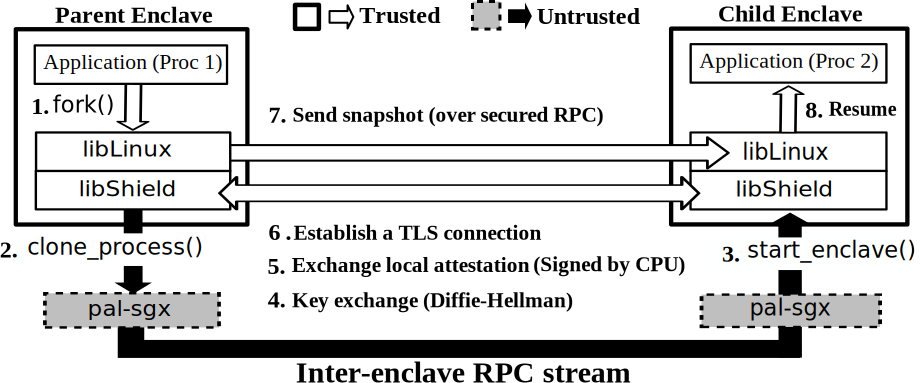
\includegraphics[width=5in]{graphene-sgx/figures/fork.pdf}
\footnotesize
\caption[Process creation in \sysname{}]
{Process creation in \sysname{}.
Numbers show the order of operations.
When a process forks, \sysname{} calls {\tt execve} system call
on the untrusted host,
to create a clean enclave with the same \libos{} image.
Then the two enclaves build up the mutual trust by
exchanging a session key, verifying attestation of each other,
and migrating the process snapshot from the parent.}
\label{fig:gsgx:fork}
\end{figure}

To secure process creation across enclaves,
\sysname{} is capable of building up the trust to newly launched enclaves,
through cooperation with an untrusted host.
Once a clean and trusted new enclave is launched,
The parent process will send a snapshot to the new one,
to create a clone of itself.
Snapshotting and migrating process states
is a feature robustly implemented and heavily used in \graphene{} \libos{},
of which we simply inherit the design.

When a process in \sysname{} forks,
because the parent and the child will be running the same binary,
both enclaves can simply be expected to have the same measurement.
To build up the trust, the two processes will open an encrypted channel
using a session key,
and exchange attestation generated by the processor.
Once both sides have confirmed the integrity of the other,
the parent process is safe to send its snapshot, encrypted, to the child
through the said channel.
The child process will restore the snapshot in its own enclave,
making it a clone of its parent.
The design of process creation in \sysname{} is shown as Figure~\ref{fig:fork}.

Forking in \sysname{} mainly defends against 3 types of attacks
from the untrusted host:

\begin{compactenum}

\item The host pretends to be the child enclave, to expose the process snapshot
sent from the parent.

\item The host pretends to be the parent enclave, to compromise the
child process using a malicious process snapshot.

\item The untrusted host becomes a man-in-the-middle, which bounces
encrypted messages between the child and parent enclaves, with session keys
negotiated with both sides.

\end{compactenum}

As described earlier, attacks 1 and 2 are prevented by mutual attestation
between the parent and the child,
and encrypting the channel for sending the snapshot.
The attestation signed by the processor proves that both entities communicating
are valid \sysname{} enclaves,
and encrypting the channel prevents the snapshot being eavesdropped or
counterfeited by the host.

To defend against attack 3 (the man-in-the-middle attack), we take advantage of
a user-customized 512-bit field
in the attestation structure generated and signed by \sgx{}.
This field is filled with a SHA-256 hash value of the agreed session key,
and the current enclave ID,
to prove that the attested enclave is the one who agrees on the key.

Once a parent enclave forks a child, by default the child must be trusted
to maintain its own security,
because the migrated snapshot discloses all information in the parent.
Unless the binary run in the parent enclave ensures
that no secrets is stored in the enclave memory at the time of snapshotting,
the parent enclave cannot simply drop the trust against the child.
For example, a pre-forked Apache web server may want to keep each worker
that responds to HTTP requests isolated,
to avoid being compromised by one attacked worker.
\graphene{} \libos{} provides an API for applications like Apache to explicitly
specify isolation to untrusted child processes.
\sysname{} inherits the ability of dynamic process isolation,
but developers are responsible for keeping confidential information
from the untrusted children.

\paragraph{Implementing {\tt execve}.}
Unlike {\tt fork}, {\tt execve} is used to
start processes with specified binaries, often different from the callers'.
When a thread in the process, either single-threaded or multi-threaded,
calls {\tt execve} in \sysname{},
\libos{} will migrate the calling thread to a new process,
with clean process states except opened files cloned from the parent.

The main challenge for implementing {\tt execve} is to
identify trusted binaries that can be loaded into new enclaves as child processes.
Consider the case where the parent process and its child shares
a multi-process abstraction (e.g., message queue).
Even if only the parent side is provisioned by the client, the child side
can still potentially compromise the secrets,
by exploiting vulnerabilities in the shared abstraction.
The trust between the parent and the child must be mutual,
unless the two enclaves are strictly isolated.

To identify binaries that can be trusted (either as parents or children)
during process creation,
\sysname{} requires each binary ported for an application,
to be shipped with a list of binaries that can be {\tt execve}'d,
and those that can be callers of {\tt execve} to the said binary.
Each binary in the list is identified by its measurement, which is mutually attested
between the parent and the child during process creation.
This list must be signed by a private key provided by the client,
while the public key must be included in the enclave measurement of the binary.

\subsection{Securing Inter-Process Coordination}
\label{sec:graphene:multiproc:ipc}

After process creation, a multi-process application often cooperate
through shared abstractions between processes,
such as signals or message queues.
For \libos{}, OS states for these shared abstractions must be shared
though inter-process coordination, for mainly two purposes.
First, for each abstraction, \libos{} needs to maintain the state
in one of its instances.
Second, \libos{} must maintain the namespace states to identify and locate the
abstraction states.

\graphene{} implements a wide range of multi-process abstractions and namespaces,
by passing messages over RPC streams among processes.
Such a design is perfect for porting multi-process applications to enclaves.
The benefit of sharing abstraction by RPC coordination are that
the enclaves will not have to share any memory to
coordinate abstraction states,
and the RPC streams can be secured by the enclaves instead of the host.

In \graphene{}, security isolation among multi-process abstractions,
regardless of their semantics,
are enforced by isolating the RPC streams used for coordination.
Unfortunately, \sysname{} cannot trust the host to faithfully isolate
the RPC streams.
Each enclave launched for an application must secure inter-process coordination
spontaneously, by only communicating to enclaves that it has attested
and exchanged secret keys with.
Because inter-process coordination is completely transparent
to the applications,
all information sent over RPC streams must be encrypted,
because \libos{} cannot determine whether the information may contain any secret.






\section{Summary}



The Linux PAL successfully leverages a limited subset of Linux system calls,
to implement the whole PAL ABI for running a
full-featured \libos{}.
\Thehostabi{} separates the development of a host OS or hypervisor
from the complexity of emulating a sufficiently-compatible
Linux kernel.
The chapter shows that most calls in \thehostabi{}
can be directly translated to similar system calls on a Linux host kernel.
Only a few \hostapis{}, such as process creation and inter-thread synchronization, require additional attention for developing an efficient implementation strategy.



The Linux PAL also enforces robust security isolation
between mutually-untrusting applications,
by placing applications in separate, VM-like sandboxes.
The security isolation on a Linux host is based on system call restriction using a \seccomp{} filter, and a trusted reference monitor. % for checking resource access.
Security isolation at the host interface
restricts an untrusted application to explore vulnerable execution paths
inside a Linux kernel.
A \seccomp{} filter 
enforce a fixed, minimal system call profile, regardless of bloated dependency of an application.
The reference monitor follows
simple, white-listed manifest rules listing 
all the authorized files and network addresses of an application,
using well-known semantics
such as AppArmor~\cite{apparmor} or iptable-like firewall rules~\cite{iptablesman}.
The reference monitor can further enforce dynamic, process-specific isolation by splitting a sandbox
to run a child \picoproc{} under more restricted
resource permissions.
\graphene{} on a Linux host can serve as a sandbox framework
with a reduced attack surface
upon the host kernel.









\makeatletter
\def\input@path{{}}
\makeatother
\graphicspath{{}}
%\chapter{\java{} Applications on SGX}
\label{chap:civet}


\newcommand{\sysname}{Civet}
\newcommand{\jvm}{JVM}
\newcommand{\jvmname}{OpenJDK 7}
\newcommand{\staticphase}{design-time}
\newcommand{\statictool}{Shredder}
\newcommand{\dynamicphase}{execution-time}
%\newcommand{\dynamicframework}{Escalator}
\newcommand{\dynamicframework}{Connector}
\newcommand{\tcbsize}{trusted code size}


\makeatletter
\newcommand{\Capitalize}[1]{%
	\edef\@tempa{\expandafter\@gobble\string#1}%
	\edef\@tempb{\expandafter\@car\@tempa\@nil}%
	\edef\@tempa{\expandafter\@cdr\@tempa\@nil}%
	\uppercase\expandafter{\expandafter\def\expandafter\@tempb\expandafter{\@tempb}}%
	\@namedef{\@tempb\@tempa}{\expandafter\MakeUppercase\expandafter{#1}}}
\makeatother

\Capitalize{\dynamicphase}
\Capitalize{\staticphase}


\makeatletter
\def\input@path{{civet/}}
\makeatother
\graphicspath{{civet/figures/}}

\begin{abstract}

  Application partitioning is a technique to move sensitive data or code into
  a protected environment, such as an SGX enclave.
  Partitioning larger existing applications requires subtle reasoning that can be aided with static
  analysis and dynamic, language-level techniques.
  For instance, in-enclave code may include a library that memoizes results in the out-of-enclave heap.
  Using a managed, type-safe language like Java in SGX also brings the benefits of partitioning to a large body of 
  existing code. %, as well as help the developer with language-level analysis tools.
  Unfortunately, running Java partitions in SGX introduces a number of technical
  challenges, many of which arise from resource and system ABI constraints.
  To our knowledge, no prior work has even run a complete Java application in an enclave,
  much less partitioned a Java application to run a piece of application logic in the enclave.
%  That said, no amount of application-level analysis can protect against
%  a compromised OS, without 
  Thus, a number of technical challenges must be addressed to unlock
  the benefit to developers of combining managed languages with hardware such as SGX.


%% \fixmets{Streamlined the argument for combining Java and SGX. Check if this makes sense.}
%% %%There have been significant, but separated %often mutually exclusive,
%% There have been significant, but often mutually exclusive
%% advances in hardware and language-level tools for partitioning applications
%% into multiple security contexts or privilege levels.
%% %Developers who build security-sensitive applications
%% %often face the dilemma of choosing between
%% %managed language features and hardware protections with language restrictions.
%% Developers either 
%% use a hardware solution, such as \intel{} \sgx{},
%% to isolate a piece of consolidated code %small piece of native binary code
%% from an untrusted OS, %but the developer
%% %must reason carefully about potential information flows that could leak data from the enclave, as well as other vulnerabilities in the code.
%% %On the other hand, in
%% or choose to program in a managed type-safe language, such as Java, 
%% %the developer has 
%% which has a wealth of tools and properties for 
%% improving code security and application partitioning.
%% %from type-checking to 
%% %more advanced tools to secure control and information flows.
%% The use of hardware
%% and language-level tools for partitioning are often complementary by concept but incompatible in reality.
%% %mutually exclusive,
%% %due to the limitations in combining the technologies.
%% %This paper observes that these language and hardware security tools 
%% %should complement each other, but are often mutually exclusive.
%% For instance, no language-level analysis %of an application
%% can protect an application against a compromised OS.
%% However, it is fundamentally challenging to
%% factor the protection of \sgx{} into the analysis of a managed type-safe language like \java{}.
%Running a managed language in an enclave is difficult, and language tools
%currently do not factor the hardware capabilities of \sgx{} or similar hardware into their analyses.


%Similarly, the \sgx{} hardware imposes restrictions on loading \java{} classes 
%with \jvm{}s;
%the \java{} language also lacks sensible APIs for using \sgx{} hardware.
%to wrap the semantic of interfaces with the 

%but are not sufficient to defend against a compromised OS or hypervisor.
%but the developer must partition the application 
%and harden the code inside the enclave.
%Managed languages, such as \java{},
%offer a wealth of language-level support for 
%but are not sufficient to defend against a compromised OS or hypervisor.
%The two approaches are often mutually-exclusive:
%we are unaware of any prior work thas has run a \jvm{} inside of an enclave at all,
%For \sgx{} and \java{},
%there is no prior work that has run a \jvm{} inside an enclave,
%much less integrated enclaves into the language's analysis tools.
%\fixmedp{check my claim. Too strong, or justified?}
%\fixmets{Since we are generalizing, we should only claim this is the case for sgx vs. Java. BTW, I prefer showing more certainty when making claims.}


%Application developers can place a library and sensitive data
%in an \intel{} \sgx{} enclave,
%but only if the library is a native binary, generally written in C.
%but must relies on developers to design invulnerable code.

%more advanced tools for detecting information flows.

%These language-level tools can be invaluable in ensuring a correct application partitioning
%and overall application correctness.
%Unfortunately, the most security-sensitive developers must choose between
%hardware and language security tools.


%% Using \intel{} \sgx{} enclaves, applications can
%% protect their most critical components from untrusted system stacks.
%% Language support for \sgx{} enclaves is a missing feature of existing \java{} Virtual Machines.
%% Using a managed language like \java{}
%% provides an opportunity to improve the weakest link of the enclave security---
%% application vulnerabilities that lead to information leakage.
%% \java{} language has effective framework to trace information flows, and provides type safety
%% to prevent memory access vulnerabilities in the enclave.
%% In addition, modularization in \java{} classes allows automatically partitioning
%% an application into enclave components,
%% minimizing the classes included in the enclave's trusted computing base.

This paper presents {\em \sysname{}},
a system that integrates \java{} language tools for partitioning applications
with run-time support for isolated execution in \sgx{} enclaves.
%\fixmedp{Any reason we can't do more than one partition in the enclave?}
%\fixmets{For an application, there is only one partition: the secure-sensitive part. We can create more than one instances in an enclave.}
%and which can execute a portion of the \java{} application in 
%a \java{} utility, runtime framework and API,
%that helps developers design isolated application components,
%and minimizes the attack vectors.
\sysname{} includes both \staticphase{} and \dynamicphase{} components.
The \staticphase{} tool, {\em \statictool{}}, uses code reachability analysis
to determine the minimal required \java{} classes for the isolated execution,
and helps the developer understand the complete partition interface. % between the application partitions.
%\sysname{} helps the developers generate an enclave image
%with minimal required \java{} classes for the protected code, reducing the TCB. %required for isolated execution.
%%\sysname{} includes language-level information flow control at the 
%%enclave border, protecting against unexpected exfiltration of secret
%%data due to application vulnerabilities.
The \dynamicphase{} framework, {\em \dynamicframework{}}, then launches the isolated execution of the enclave image
(a signed JAR archive) in an enclave when the untrusted part calls the interface.
Throughout the execution, \sysname{} enforces end-to-end isolation
on any object instantiated inside the enclave,
and leverages language-level information flow control to determine whether an object contains no sensitive information before the object is released from the enclave.
%to protect against unexpected ex-filtration of secret
%data. % due to application vulnerabilities.
%\fixmebj{How about this?}
%\fixmedp{Is this best-effort?  Only for explicit flows?  The 
%preceding sentence should be crisper}
%identifies information flow at the enclave border,
%preventing enclave secrets
%from being leaked due to any vulnerabilities.
%with minimal classes needed for the isolated computation,
%and narrowest interface for interaction.
%Second, the framework effectively prevents information leakage
%by forbidding any objects tainted by information flow to leave the enclave.
%In \sysname{},
%trusted servers may provision secure objects and classes,
%preserving security policy information. \fixmedp{Don't understand the previous sentence}
%\fixmedp{Do we want to say anything about contributing techniques to get good performance?}
%To secure \java{} applications, 
%With both the \staticphase{} and \dynamicphase{} language support,
\sysname{} also creates language-level abstractions of and extensions \sgx{},
such as attestation and provisioning, simplifying cumbersome aspects of this hardware
for developers.
%extends the security properties (e.g., data confidentiality) and features (e.g., attestation and provisioning)
%of \sgx{}, %hardware protection to cover \java{} classes dynamically loaded by the \jvm{},
%and encapsulates cumbersome aspects of interfacing with the hardware architecture
%keeps the work of bootstrapping and interfacing with 
%from application developers.
%As a proof-of-concept of using advanced language-level tools,
%we use \sysname{} %strengthens hardware protection
%to identify and remove 
%by filtering 
%implicit information flows that would leak secrets from an enclave
 % that leaks secrets
%in our test applications.
%\fixmedp{all of them?  Or just one?}\fixmets{I think this technique applies to all test cases.} % error-prone applications. 
%Finally, the API allows components in enclaves to be seamlessly provisioned with
%secure objects or classes by trusted servers,
%and to preserve their security policy information.
%with security guarantees extended from their sources.
%\sysname{} is evaluated with \jvmname{} on the latest 
%We evaluate \sysname{} % with several case studies 
%on the latest \intel{} Skylake processor.
%Evaluation shows good performance on
%Our overheads are low, 
%adding \fixmedp{xx}\% overhead on an isolated cryptographic library used in SSH client/server,
%and \fixmedp{xx}\% overhead on Hadoop jobs that run a secret, provisioned algorithm.
We demonstrate the usage of \sysname{} with two applications: a SSH server with an isolated cryptographic library to protect its host key,
and a Hadoop framework capable of securely executing jobs using any secret, provisioned algorithm.
%\sysname{} reduces the developer effort required to partition the application code,
%resulting in a smaller 
%and the result of integration is highly generalizable to other managed languages.
%~\fixmebj{Always replace TCB with code footprint size to indicate that we are only talking about size of code - not attack vectors.}
%\fixmets{find a better term for TCB size}
%~\fixmebj{Always replace managed languages with managed type-safe languages.}
%\fixmets{accurately separate managed language and type-safety: managed language causes the challenges, and type-safety improves the security properties; Java happens to be both.
%}
\end{abstract}

This chapter describes the formal definition of the \graphene{} host ABI.

\section{Basic Definitions}

The \graphene{} host ABI defines a set of {\em functions}, similar to the API of UNIX or POSIX.
The functions are directly called by the library OS, along with the arguments given either in the registers or on the stack.
A host-specific \graphene{} loader is responsible for resolving the linking, from the library OS to the host ABI.
%\papersection{Challenges for Partitioning with Enclaves}
\label{sec:background}
In this section, we will give a brief overview of \sgx{}, and discuss 
the key challenges developers face when trying to manually partition applications using a technology such as \sgx{}.
%discuss the programming models and threats to security of \sgx{} enclaves.

\papersubsection{Background on \intel{} \sgx{} Enclaves}

\intel{} \sgx{} ({\it Software Guard Extension})
is a set of new x86/x64 instructions
introduced in the \intel{} Skylake processor family.
Using \sgx{}, an 
application can designate part of its virtual memory as an {\em enclave}.
The CPU guarantees that the contents of the enclave never leave the CPU package unencrypted.
The CPU also measures the integrity of a binary loaded into the enclave, and offers remote attestation,
similar to a TPM\fixmedp{cite}.

%%% create a protected memory region, called an {\em enclave}, inside it's virtual memory,
%%% where it can load its security sensitive data with hardware-enforced isolation from the untrusted OS. 
%%% The processor with \sgx{}
%%% guarantees that any data loaded in enclave
%%% stays encrypted in the DRAM, by using a secret key deterministically derived from the application's cryptographic measurement and the CPU secret. 

\sgx{} is an appealing tool for protecting small amounts of highly-sensitive data or code, because it can defend 
against a malicious or compromsed OS, hypervisor, or even hardware peripheral.
For instance, \fixmedp{Foo} et al.~\fixmedp{cite that \sgx{} workshop paper} show how \sgx{} can be used
to build a trusted path from a video chat application to a GPU and network card, which maintains confidentiality and integrity of the
video stream, even if the OS is compromised.
Simlarly, because DRAM contents are encrypted, \sgx{} can resist cold-boot attacks~\cite{halderman09coldboot} or 
malicious peripheral devices~\cite{hudson15thunderstrike}.


%%% \sgx{} also proves the integrity of loaded binaries to remote trusted entities
%%% using mutual attestation based on a symmetric key generated from the measurements of communicating entities.
%%% \sgx{} usage model mostly involve the launched enclave mutually attesting the trusted host
%%% to obtain provisioning of security-sensitive information
%%% through a trusted channel. Such an execution model leverages resources such as CPU and DRAM from vulnerable untrusted \sgx{}-enabled hosts owned by cloud providers
%%% by extending the trust from
%%% the hosts owned and trusted by the clients or service providers.
%%% For instance, \sgx{} can isolate the decoder engine in an enclave
%%% after authenticating the customers to enforce Digital Right Management (DRM) even if the digital data is hosted on an untrusted cloud server.

%Use cases of \sgx{} mostly involve the launched enclave
%retrieving a cryptographically signed attestation from the processor,
%to exchange security critical information with remote servers through secured channels.
%The effect is equivalent to expanding the trusted space from remote servers
%to the local end, to harness local resources such as CPU and DRAM.

%One must note that \sgx{} only promises the integrity of application binaries
%initially loaded in enclaves.
%The gap between integrity of binaries and complete security has to be filled
%by ones who develop and approve the applications.
%More specifically, the clients are responsible of
%testing whether the applications contain any vulnerabilities
%that lead to information leak.
%To minimize the risk of leaving any flaws in the applications unintentionally,
%developers often tend to cut down the trusted computing base (TCB)
%of the applications. With smaller TCB, clients who launched the enclaves
%can more easily reason about the thoroughness of securing the execution.

%%% The key strength of \sgx{} enclaves over other software-based isolation framework such as
%%% {\em Flicker}, {\em Inktag} or {\em Virtual Ghost} is
%%% the ability to defend against attacks at the hardware level.
%%% These software-based solution often
%%% rely on a hypervisor below the OS to isolate the applications.
%%% If the hardware is attacked,
%%% the attackers may still bypass the software checkpoints,
%%% or directly steal confidential information from the DRAM.
%%% For \sgx{}, the only hardware included in the TCB is the CPU package,
%%% and in practice CPUs are believed to be hard to attack.
%%% Using techniques like cold-boot attacks~\cite{halderman09coldboot}
%%% to peek into DRAM content,
%%% or intruding the boot process using corrupted peripheral devices like Thuderstrike~\cite{hudson15thunderstrike}
%%% will affect any software-based isolation, but not \sgx{} enclaves.

\paragraph{Non-Partitioned Applications.}
One approach to using \sgx{} is to run an entire application in the enclave.
This is exemplified by Haven~\cite{baumann14haven}, which runs a \win{} application and all supporting libraries
on top of a {\em library OS}.  This approach is illustrated on the left side of Figure~\ref{fig:libosvssdk}.
The library OS approach does not require any application changes, but bloats the TCB \fixmedp{Rough number of how big Haven is}.
By pulling millions of lines of extraneous code into an enclave, there is a significantly increased risk 
of vulnerabilities that disclose
sensitive data, such as Heartbleed~\fixmedp{cite}.
The library OS approach is useful in its simplicity of deployment and can provide practical benefits, 
such as protecting an application from an untrusted cloud hypervisor.

\begin{figure}[t!]
\centering
\includegraphics[width=\linewidth]{figures/libosvssdk.pdf}
\footnotesize
\vspace{-0.2in}
\caption{
Comparison between the libOS-based model (e.g., Haven)
and the partitioned model for programing applications in enclaves.
Green (light) boxes are trusted components and red (dark) boxes are untrusted.
The libOS-based model yields a larger TCB in the enclave,
while the partitioned model requires developers to be responsible for determining the untrusted interface at the enclave boundary.
}
\label{fig:libosvssdk}
\end{figure}


This paper focuses on a second usage model for enclaves, where the application is partitioned into
untrusted and one or more trusted components (right side of Figure~\ref{fig:libosvssdk}).
Sensitive data and computation are placed inside of enclaves.  This approach requires the developer to
identify sensitive code and data; design and harden an interface between trusted and untrusted components; 
modify the application source; and reason about potential information flows at the enclave boundary.
This effort can be non-trivial and subtle, but for application developers motivated by interests such as 
regulatory compliance or competitive advantage in business, the additional effort can yield a much smaller trusted computing
base (TCB), and thus a reduced attack surface.
A key goal of \sysname{} is to minimize the developer's effort to partition an application---both in lines of 
code changed, and in leveraging language analysis to reason about narrow points in the application's data and control flow.


%To achieve smaller TCB, the software development kit of \sgx{}
%intends to encourage developers to partition the applications and
%keep only security sensitive components in the enclaves.
%Such an intention is exactly contradicted by the trust model of \haven{},
%which must trust the loaded application as a whole.
%Except for the cases in which the whole applications must be secured,
%\haven{} actually downgrades the trustworthiness of enclaves.
%Figure~\ref{fig:libosvssdk} shows the comparison of the two models.

%%% In prior works using \sgx{} enclaves to secure applications,
%%% developers choose between two different programing models: the {\em library-OS-based} and the {\em partitioned} model (as shown in Figure~\ref{fig:libosvssdk}).
%%% In the libOS-based model, developers run the whole standalone,
%%% legacy application inside the enclave, using library OS such as {\em Haven} or {\em Graphene libOS} to facilitate the rich OS features.
%%% The main benefit of using library OS is that developers only have to employ minimal efforts to port any existing application.
%%% Even when designing new applications, developers bear no responsibility
%%% of identifying and reasoning about
%%% the security sensitive part of the application.

%%% However, when using libOS-based model, a sophisticated legacy application
%%% will yield huge trusted computing base (TCB) in the enclave,
%%% aggravating the risk of leaking information through vulnerabilities inside the enclave.
%%% Known bugs such as {\em the heart-bleeding bug} has shown that
%%% running security sensitive code like an encryption engine, and management code such as heart-beating service in the same address space
%%% can cause vulnerabilities that compromise the security by leaking the encryption key.
%%% As a result, using a partitioned model, developers can isolate only the most security sensitive components in an enclave,
%%% and leave the remaining code outside to minimize the TCB.

%%% Developers have to define the {\em untrusted interface} 
%%% to allow parts of a partitioned applications to interact.
%%% The untrusted interface is used either by the the untrusted components
%%% to trigger execution of the isolated components,
%%% or by isolated components to use untrusted rich OS features, such as networking for provisioning and sending the execution output to the remote hosts.
%%% Unlike the libOS approach that has a fixed untrusted interface (for different applications) at their interaction boundary with the OS,
%%% the width of untrusted interface for a partitioned application is up to developers' design.
%%% The \intel{} SDK for \sgx{} supports a set of syntaxes to specify the type and direction of flow for parameters of the untrusted interface, and enforces primitive
%%% type-checking of incoming values on transition to enclave.

%%% The trade-off between the libOS-based and partition model is based 
%%% on ease of development, the width of untrusted interface,
%%% and size of TCB.
%%% The benefit of the libOS-based model is that developers can save the effort
%%% of determining what to execute in the enclave,
%%% and whether the execution is safe,
%%% because the whole application is wrapped in the enclave.
%%% However, the risk of having vulnerabilities in the applications
%%% is not reduced, but in fact amplified due to the addition of
%%% the library OS (e.g., the Haven binary yields around a few hundred MBs) to TCB.
%%% On the other hand, if the developers are willing to spend effort on carefully identifying the untrusted interface and re-designing their application around this interface, the partitioned model can improve security guarantees by minimizing the attack vectors.

%%% The goal of \sysname{} is to provide the benefits of both models.
%%% \sysname{} support a partitioned model
%%% for developers to isolate security-sensitive part of a \java{} application in enclave,
%%% and provide a language-based tool to automatically partition
%%% the minimal supporting classes to generate the enclave image.
%%% Even in the case where the isolated component need to frequently interact with the untrusted component or the OS,
%%% the language protection technique of information flow tracking
%%% guarantees that the secrets in the enclave are never leaked
%%% without the developers explicit consent. 

\paragraph{Side Channels and Denial-of-Service.}
In the current \sgx{} design, side channels are a signficant concern for either the library OS or partitioned model, and are out of the scope of this paper.
A controlled channel attack~\fixmedp{cite} can single step enclave execution by inducing page faults
in the enclave.  \sysname{} does not specifically defend against side channel attacks,
and we expect that any solution to this problem involves redesigning the division of labor in virtual
memory management for enclaves.

Similarly, there is no guarantee that a compromised application will ever enter
an enclave.  Denial-of-service attacks are out of scope for this paper.


\papersubsection{Challenges for Application Partitioning on \sgx{}}

\sgx{} provides useful building blocks for secure applications, but does not
absolve the programmer of any responsibility for reasoning about end-to-end security.
Bugs in the application or supporting libraries can still disclose sensitive data from an enclave,
and porting code into \sgx{} can be subtle.
This subsection outlines several pitfalls in partitioning an application for \sgx{}.

%%% \sgx{} enclaves provide strong isolation guarantee for applications,
%%% against the malicious or vulnerable application components, system stack,
%%% and hardware (except the CPU itself).
%%% However, the security guarantees of the \sgx{} enclave is dependent on whether the developers design perfect applications without exploitable vulnerabilities that may compromise the application's security.
%%% As the application developers are not perfect,
%%% even applications or components isolated in enclave can face threats to their security.
%%% As follows, we discuss a few potential threats
%%% to the enclave security,
%%% even under the assumption that the \sgx{} hardware is implemented as completely secure --- which can be another threat otherwise. 

%\fixmedp{I roughly want the rest of this section to have a problem, explanation, solution structure, with the overall theme being that this is subtle and we really need some analysis tools to get this right}

\paragraph{Writes outside of the enclave.}
\sgx{} allows code inside the enclave to read and write data structures 
outside of the enclave.  Thus, it is easy for a developer to inadvertently write
code that discloses a secret, say by using a library that memoizes intermediate results to the untrusted heap.
A fundamental requirement is that developers must be able to reason about (or assert)
what code can and can't access data {\em outside} of the enclave.
\fixmedp{Can we say anything about whether such tools exist before Civet?}

%\fixmedp{Do I recall correctly that you can easily write to data outside of the enclave?  If so, this seems like something easy to get wrong, especially 
%if a library memoizes intermediate results.  The developer needs to be able to tell 
%Unless I am full of shit, can we paragraph-ize this fixme?

\paragraph{Application vulnerabilities.} 
The major source of threats to enclave security is any internal vulnerabilities in the isolated components,
such as buffer overflows and other memory corruption attacks.
Moreover, although \sgx{} code integrity guarantees make enclaves resistant to code injection,
an attacker may still manipulate control flow using code-reuse attacks~\cite{code-reuse-attacks}.
Moreover, recent research ~\cite{hudata} show that even with perfect control flow integrity,
attackers can still manipulate the execution to leak the secrets through information flow.

Fundamentally, this argues for some combination of static analysis
and runtime monitoring of 
enclave code.  This is greatly simplified when the enclave code is written in higher-level languages
with properties 
%amenable to analysis.
%with type safety, memory safety, and other 
%that provide important 
%safety properties,
such as type safety or memory safety. %, thereby reducing the likelihood of these vulnerabilities.
Ideally, one would formally verify security properties of enclave code~\cite{moat}; this verification is significantly aided by using 
higher-level languages amenable to formal reasoning.
%Verification is significantly harder
%with C or x86 assembly.

%% \paragraph{Applications are not perfect} 
%% The \sgx{} hardware cannot prevent applications from copying secrets out of the enclave without limiting functionality.
%% The trusted isolated components can copy any sensitive data from the enclave to the unencrypted memory, and potentially leak the enclave secrets.
%% The primary risk in the isolated components
%% is often memory corruption vulnerabilities, such as buffer overflow,
%% %Because in enclave applications can access any part of out-of-enclave memory unrestrictedly,
%% prevalent in applications that are not implemented in type-safe languages.

%% The best known technique to prevent vulnerabilities is to model the applications and verify them using {\em formal verification}.
%% While Sinha et.al.,~\cite{moat} use formal verification to prove confidentiality of enclave programs, it is impractical to accurately model complex sophisticated applications.
%% As a result, in addition to formal verification, maintaining smallest TCB
%% in the isolated components is the most practical approach 
%% to ensure enclave security,
%% and is the main reason to choose partitioned programming model over
%% libOS-based model.


\begin{figure}[t!]
\centering
\includegraphics[width=\linewidth]{figures/partition.pdf}
\footnotesize
\vspace{-0.3in}
\caption{
Partitioning --- either manually or by automated tool ---
often causes wider boundary of partition than the actual security sensitivity boundary
due to (a) design granularity : {\tt secHelper} contains a {\tt send()} method that is not partitioned from the rest of the class by design.
The reasons of having the gap vary, for instance, 
that is less security sensitive, but due to the granularity it is not partitioned from the rest of the class or (b) better performance :  the less security sensitive {\tt logger} class is kept in the privileged level to service frequent method calls.
}
\label{fig:partition}
\end{figure}

%However, even if developers partition the applications and run only
%security sensitive components in the enclave,
%the developers may still leave some code irrelevant to
%enclave secrets inside the enclave.
%The reasons of having more-than-minimal TCB in enclaves
%are often that developers have to partition code in the granularity of source files or functions,
%or developers have to import more code to limit the width of interface and
%the frequency of interaction with the untrusted code.

\paragraph{Identifying ``pinch points''.}
Reasoning about where in a program to draw the line between 
trusted and untrusted code is subtle.
On one hand, the developer has an incentive to minimize the size of the 
API between the enclave and untrusted code, as well as an incentive to
minimize the total code in the enclave.  These goals can sometimes be at odds.
Each entry and exit to an enclave has a cost roughly comparable to a
process context switch\fixmedp{right?}; an easy way to reduce enclave entries and exits is to simply 
pull more code into the enclave, which increases the size of the TCB.

\fixmedp{I'm not sure how to explain Figure~\ref{fig:partition}, but it needs an explanation.}

Fundamentally, the art of paritioning an application is to find a ``pinch point'' or
``narrow waist'' in the application, where there is a natural point to insert an API and 
security checks.  This is indeed as much art as science, often done manually by experts\fixmedp{any more supporting evidence or cites?}.
It is unlikely that the average developer will successfully navigate this design process without analysis tools, such as \fixmedp{examples?},
to help identify these natural division points.


%% Experts can use a manual partitioning technique to achieve smallest TCB for the isolated components compared to automated tools.
%% However, the manual partitioning costs a lot of effort,
%% and rare expertise, lack of which can cause larger TCB.

%% Neither manual nor automated partitioning is perfect:
%% the resulted boundary of partitioning often has a gap from the actual boundary of security sensitivity (as shown in figure~\ref{fig:partition}),
%% leaving more code in the privileged level
%% than what's actually needed.
%% Having the gap between the ideal and resulted boundary
%% is mostly inevitable, due to multiple reasons.
%% One common reason is the granularity of partitioning,
%% which can vary from a binary file, a component, a source file,
%% a class, a method (a function) to a line of code.
%% Another reason is that a component or a method may be too frequently called
%% by the security sensitive code,
%% laying the boundary between the component or method from the security sensitive side may bring too much overhead or risk,
%% because the execution crosses the boundary too often.
%% Therefore, developers often will balance among the effort of partitioning,
%% risk or cost of communicating between different partitions,
%% and minimizing the TCB in the security sensitive parts.

\fixmedp{Maybe move the commented paragraph below down into the design section?  I'd like to downplay the plugs for our work here, and instead fulfill these promises later}
%% \sysname{} automates partitioning of applications,
%% based on the boundary at the classes which the developers marked
%% as the interfaces of the enclave.
%% Only the classes that are depended by the marked classes
%% will be included in the enclaves,
%% to minimize the TCB.
%% Although not all classes pulled into the enclaves
%% are necessarily security sensitive,
%% the enclaves are protected from the potential vulnerabilities in those classes,
%% by the security guarantees of \java{} language,
%% and the information flow tracking in \sysname{}.

%Another threat to \sgx{} is the vulnerability of the 
%security sensitive code running in the Enclave. The 
%main guarantee of \sgx{} to isolate the secure data 
%from other components and privileged OS is undermined 
%if the Enclave code can be tricked to leak the 
%security sensitive data to the attacker. Executing 
%buggy code in \sgx{} enclave can inadvertently leak 
%information if the attacker can exploit memory-safety 
%vulnerabilities like buffer overflow and dangling 
%pointers.  

% Cumbersome and approximation to partition code
%The developers have to manually partition their code 
%into security sensitive and insensitive part. If this 
%partitioning is done by a novice developer, some of 
%the security insensitive parts of the application can 
%end up in the security sensitive part, increasing the 
%Trusted Computing Base(TCB). Moreover, the 
%partitioning of code is not straightforward, which 
%can also contribute to a less stricter TCB. The bigger the TCB, the more %vulnerable is the Enclave code to attacks.

% Buggy Code leads to inadvertant information leakage


% \sgx{} code only Integrity protected not confidential
%Moreover, \sgx{} only protects the integrity of the enclave code. The security critical part of the application is stored in plaintext while the secret data is provisioned securely after attestation. However, \sgx{} does not protect the confidentiality of enclave application code which may be executing a secret algorithm. \fixmebj{Talk more about the problem motivating security tag preservation.}
%\sgx{} can natively guarantee either code integrity or
%code confidentiality (as part of the enclave data), but not both.
%If application code is included in the enclave measurement and
%verified by the hardware,
%the code must stay in plaintext as part of the enclave image.
%If any code is stored or provisioned in encrypted forms,
%the application or infrastructure in enclave must dynamically load
%the code after decryption.
%Supporting dynamic loading makes enclaves open to code injection
%if the applications have exploitable vulnerabilities.

\paragraph{Code Integrity {\em and} Confidentiality.} 
The hardware-level \sgx{} code integrity mechanism is based on a cryptographic
signature of a static binary in plaintext.
If any application dynamically loads any code after the enclave's initial measurement,
the initial application must be trusted to attest the loaded code.
The subtle tension is that there is no way to protect the confidentiality of
a secret algorithm, except by dynamically loading an encrypted binary.
Dynamically loading code increases the risk of code injection attacks and other control flow compromises.

Any application partitioning solution that protects sensitive algorithms
must have a robust dynamic loader that can measure encrypted libraries or classes.
\sysname{} includes a loader that can measure encrypted class files,
provisioned from a trusted host.

%% \sgx{} enclaves require code integrity in the isolated applications.
%% If the code integrity is not maintained, adversaries can corrupt the enclave code to
%% force the applications to leak the information provisioned from the remote,
%% trusted hosts.
%% \sgx{} hardware only guarantees
%% the integrity of the code initially loaded into the enclaves.
%% However, if an application choose to dynamically
%% load any code after the enclave starts,
%% the application is responsible for the integrity of the code loaded.
%% The fact that dynamic loading of applications, libraries or components
%% is a feature that can potentially make enclaves vulnerable and open to code injection,
%% raises concerns against supporting managed languages in the enclaves.

%% On the other hand, code confidentiality can be a desirable feature,
%% for application developers who prefer keeping the secret sauce of their algorithms concealed.
%% To enable the feature of code confidentiality in enclaves, the protected code must be dynamically loaded into the enclave,
%% because the \sgx{} hardware only accept
%% the initial loaded code to be in plaintext.
%% \sysname{} provides both code integrity and confidentiality by verifying
%% every classes dynamically loaded into the enclaves,
%% and allows loading classes provisioned from trusted hosts.


%% In general \sgx{} enclaves are prone to having side channels, such as timing channels. Because \sgx{} relies on the untrusted OS for paging,
%% an enclave will always leak page fault addresses, except the lower 12 bits (offsets in pages).
%% Such a leakage gives the untrusted OS to amplify the side channels,
%% by forcing page faults on every instruction or memory access.
%% This so-called {\em Controlled Channel Attack} is common to all applications who use \sgx{} protection, regardless of the programming models.
%% \sysname{} does not specifically defend against side channel attacks.

%% \paragraph{Denial-Of-Service Attacks}
%% \sgx{} is not designed to be safe against denial-of-service attacks.
%% Because the untrusted OS still controls the host resources,
%% there are countless ways to prevent an enclave from making progress.
%% For example, the OS can simply starve the enclaves by
%% never scheduling CPU, memory or other resources to the enclaves.
%% \sysname{} does not specifically defend against denial-of-service attacks.

\paragraph{Discussion.}  This
section has outlined several pitfalls for developers of partitioned applications.
These common pitfalls render the hardware protections of \sgx{} useless.
Language-level analysis can automate error-prone reasoning in the best case, or, in the worst case, 
can at least offer invaluable guidance to the developer.  For \sgx{}-style
hardware to be useful to a wide array of developers, developers need language-level
tools that can also factor in hardware-level protection mechanisms.



%- Motivate the problem.
%- List all attack vectors
%- How can JAVA help?




















































































\input{background2}
%\section{Threat Model}
\label{sec:threat}

In this section, we discuss the threat model of \sysname{},
including the adversaries,
and the components that must be trusted.

\paragraph{Adversaries}
We assume the same adversaries as other \sgx{} enclaves.
Any part of the system stacks, including the OSes,
device drivers, hypervisors, and even hardware,
such DRAM, GPU, buses, and peripheral devices, can be malicious
and attempt to attack the enclaves.
%The only trusted component is the CPU package, including L2 and L3 caches.
The attackers can perform any form of
online and offline attacks.
We also assume the attackers own all information
about \sgx{} hardware implementation, as well as every part of our solution.

We focus on the adversaries that target on
exploiting vulnerabilities in the isolated applications.
The attackers can manipulate any input to the application interfaces,
or the untrusted interfaces of the enclaves.
%Attackers may apply any techniques that compromise a regular privileged applications to compromise enclaves.
The vulnerabilities that attackers can exploit may not only fall in applications, but also in the infrastructures,
such as the libOS, the \java{} VM, JNIs and low-level interface to architecture.

%The only adversaries that are not addressed in \sysname{} are
%attackers exploiting {\em side channels} and
%{\em denial-of-service attacks}.
%Side channels, or even controlled channels, is a known problem of \sgx{} enclave
%and we expect to solve the problem in the future with
%stronger architectural support.
%Denial-of-service attacks are often considered benign for enclaves,
%because it only affect the ability of an untrusted host to legally access
%critical resources.

\paragraph{Trusted Components}
We trust any components loaded inside an enclave,
including the infrastructure (details discussed in Section~\ref{sec:implementation}), %(low-level interface, the libOS, \jvmname{}),
all supporting classes and their JNI,
and other resources or classes provisioned from remote hosts.
%All trusted components must be verified by either \sgx{} hardware or the infrastructure against their cryptographical measurements or checksums.
The implementation of \sgx{} hardware is also trusted to be invulnerable,
and use adversary-resistant key generators that cannot be compromised
by online or offline techniques.
We also assume \intel{} CPUs are resistant to direct, physical attack to the CPU packages, either to modify or peek into the chips.

\fixmets{Now JIT'ed code is not giving me error, but in case it fails later, we have to flip this discussion.}
We support running \java{} application both with and without JIT optimization.
Running \java{} application with JIT optimization
improve the performance of execution,
but can cause massive increase of the TCB of enclaves.
In case that JIT optimization is enabled in the enclaves,
the JIT compilers (\java{} VMs often have multiple JIT compilers, e.g., \jvmname{} has two) must be trusted by the users,
to always generate correct and invulnerable binary code.


%Note that in \sysname{} we disable JIT compiler that used to improve \java{} execution performance.
%The choice of disabling runtime compilation is due to the concerns that
%JIT compiler may largely extend the TCB because it must be trusted,
%and any bugs in different versions of compilers
%may causes code behaviors than what developers have tested and expect.
%Another practical reason is concerning the complexity and
%resources required for running a \java{} compiler with library OS in an %enclave.
%However, we consider these limitations to be not fundamental to the approach, and we keep compiler support in \sysname{} as a future work.



%In term of architecture, we trust the implementation of \sgx{} hardware,
%to maintain invulnerable implementation of \sgx{} instructions,
%and using adversary-resistant key generators that cannot be compromised
%by attacker using online or offline techniques.
%The CPU must keep enclave contents encrypted in DRAM and low-level caches that are shared by multiple cores.
%We also assume \intel{} CPUs are resistant to direct, physical attack to the CPU packages, either to modify or peek into the packages.

%\sysname{} protects confidentiality and integrity of provisioned security critical data in the trusted part of an application written in a high level managed language like JAVA.
% from the privileged operating system and the untrusted part of the same application. 
%\sysname{} assumes that the \sgx{} instructions are implemented correctly in the processor, and the SDK do not contain exploitable bugs to leak information. In addition, \sysname{} trusts the Graphene LibOS and the JVM running in the enclave with the trusted part of the application to not leak information. Thus, the security of the provisioned data is limited by the correctness of the processor, \sgx{}, Graphene LibOS, and JVM. \sysname{} also trusts the trusted part of the application to not leak information explicitly. \sysname{} prevents the trusted part of an application from implicitly leaking information.

%Threats that we do not cover
%\sysname{} inherits the threat model of \sgx{}~\cite{sgx}.
%The adversary controls the cloud provider's complete stack, OS, hypervisor, BIOS, system management mode, platform firmware, and device firmware. The adversary can also probe the memory and manipulate the I/O, but cannot read secret present in the processor.
%\sysname{} do not defend against attack vectors such as side-channel, covert-channel and control-channel~\cite{control-channel}. Denial of Service (DOS) attack is not part of \sysname's threat model. Even if the OS never schedules the enclave program or the untrusted part of the application is manipulated to never enter the enclave, no provisioned secret is leaked outside the enclave.


\papersection{Overview of the \sysname{} System}
\label{sec:overview}

This section provides an overview of \sysname{},
a system that assists developers in partitioning \java{} applications,
by combining \sgx{} hardware protection and \java{} analysis tools.
%with hardened security from both \sgx{}'s security guarantees and 
%\java{}'s safety features.
%% dep
%We will also discuss the threat model assumed in the design of \sysname{}.

\begin{comment}

%\begin{figure}[t!]
%	\centering
%	\includegraphics[width=\linewidth]{figures/alternatives.pdf}
%	\footnotesize
%	\caption{Alternative approaches to access \sgx{} hardware protection from \java{} applications.
%		The {\em libOS-based} approach runs the whole \java{} applications in the enclaves. 
%		The {\em JNI-based} approach uses JNI to run the security sensitive operations inside the enclaves.
%		The {\em \jvm{}-based} approach requires the \jvm{} to provide APIs to support common use cases of the enclaves.
%		Green (light) boxes are trusted components and red (dark) boxes are untrusted.
%	}
%	\label{fig:alternatives}
%\end{figure}

There are multiple approaches to access \sgx{} hardware from \java{} applications as illustrated in Figure~\ref{fig:alternatives}. Firstly, the whole \java{} application can run with the \jvm{} inside the enclaves,
using a \sgx{} like Haven~\cite{baumann14haven}({\em libOS-based}).
Secondly, the untrusted components of \java{} application
can run with the \jvm{} outside the enclaves, and a JNI wrapper can communicate
with the trusted component written in native language running inside the enclave like ~\cite{vc3}({\em JNI-based}). 
However,the JNI-based approach requires developers to have the knowledge of
enclave implementation, and loses the language protection of \java{} inside the enclaves.
A more plausible approach is to provide enclave-backed APIs
from the \jvm{},
to support common use cases ({\em \jvm{}-based})), such as a secure key-value store~\cite{vc3}.
Although the \jvm{}-based approach can save the application developers' effort
of implementing isolated components,
the use cases is limited to the pre-defined operations provided by the \jvm{} or the companion frameworks.
Because the backend implementation (isolated components and untrusted interfaces) in the \jvm{}-based approach is the same as the JNI-based approach,
the same language restriction also applies here. 

\end{comment}

\papersubsection{Design and Features}

\sysname{} consists of a \staticphase{} tool (\statictool{}) and a \dynamicphase{} framework (\dynamicframework{}):
%to help 
%developers to partition \java{} applications.

\paragraph{Partitioning \java{} applications into enclaves (\statictool{})}
To cleanly partition \java{} applications into
 trusted and untrusted components,
 \sysname{} provides a \staticphase{} tool called \statictool{}
%\fixmedp{I recommend naming each component: ``Shredder'' vs. ``the Civet design-time tool''} 
 to automate partitioning.
 In a \sysname{} partition, there are three types of classes.
 First, the developer will identify trusted classes that must execute
 exclusively in the enclave, called an entry class.
 \statictool{}  will identify functions and supporting classes that are reachable
 from the enclave.
 The developer will then decide which additional classes can be instantiated
 only in the enclave, which can be instantiated inside and outside of the enclave, and
 which can only be created outside of the enclave---essentially forming a border
 for the partition.
%The developer manually identifies trusted classes that should be placed in the enclave,
%but will still interact with untrusted components.
%These classes are called entry classes for the enclave.
%Based on the list of entry classes, 
%Shredder selects all supporting classes required by the entry classes,
%the minimal supporting classes that the entry classes have dependency against,
 \statictool{} creates a static image of the in-enclave java classes, packaged as a signed JAR file.
 
 \sysname{} partitions at class granularity, but enforces isolation at  object-level.
 In other words, some classes can execute both in and out of the enclave,
 such as a generic container class or the String class; in these cases,
 the runtime isolation granularity is  object-level (whether it is placed
 in the enclave heap or the untrusted heap).
 \sysname{} does not currently remove unused functions from in-enclave classes,
 although this enhancement could be adopted in future work.
  

%The developer can request for other non-sensitive classes or packages to also be included in the enclave JAR file.
%\fixmedp{Can the developer override this if she wants to exclude some packages, or replicate some packages, rather than share them?  What if she wants instances of the same class in and out of the enclave?}


% \fixmebj{Talk about class level partition granularity and object level isolation granularity.}
%\sysname{} asks the developers to identifies the trusted classes that must be isolated in the enclave,
%but interact with the untrusted components.

For most cases, \sysname{} only requires the developers
to identify the entry classes, and, as desired, to annotate declassifiers for information flow tracking (\S\ref{sec:concept:accessing}).
Our goal is to minimize developer effort required to partition the application.
%This approach minimizes the developer effort 
%The design-time tool of \sysname{} largely reduces the cost of partitioning applications into enclaves.

%In \sysname{}, the developer identifies 
%trusted classes that store
%security sensitive data or code. 
%\fixmedp{Can we say something more crisp about the annotation process.  Maybe related it to the Isolated class definition?}
%Based on the developer's annotations,
%the \sysname{} utility \fixmedp{can we name the pieces?}
%automatically partitions the application into two parts:
%an enclave image and the untrusted image of the application. 
%\fixmedp{I thought the partitioning would be more developer-guided.  
%is the partitioning totally automatic?  Can the developer refine?}
%The enclave includes both annotated classes and classes required by 
%the annotated classes. \fixmedp{Is it just a transitive closure dependency analysis?  Is there ever a case where a class is kept out of the enclave?}
%The \sysname{} utility also creates an interface between the untrusted 
%code, entry points for the enclave, and signs a measurement of 
%the trusted components.

%%% The enclave includes only 
%%% the classes required by  that are depended by the marked classes
%%% are included in the enclaves,
%%% to achieve the golden mean of minimizing the TCB and optimizing performance.


%%% \sysname{} provides application developers with a utility that automatically partitions the application into two parts --- 

%%% \sysname{} statically create entry points for the untrusted interface, and signs the measurement of the trusted components. 


%%%  developers 
%%% partition their code, and provides runtime support to securely and 
%%% seamlessly run trusted components in \sgx{}.
\paragraph{Triggering enclave execution for partitioned \java{} classes (\dynamicframework{})}
To seamlessly trigger enclave execution and access in-enclave objects,
\sysname{} provides a \dynamicphase{} framework called \dynamicframework{} to load the partitioned \java{} classes into enclaves.
% and make \sgx{} protection guarantees first class components of the \java{} language.
%When \sysname{} is called to run isolated \java{} components,
\dynamicframework{} creates two \java{} execution environments: 
one in the enclave (\emph{trusted}) and one outside the enclave (\emph{untrusted}), as illustrated in Figure~\ref{fig:synthesis}.
%Both environments have an individual \jvm{}.
The \jvm{} outside the enclave is the default \jvm{}; the \jvm{} inside the enclave is a lightweight \jvm{},
with just enough features to support the trusted components but a smaller TCB.
%The lightweight \jvm{} runs in a an enclave \sgx{}.
%\dynamicframework{} abstracts the low-level semantics of the \sgx{} hardware from the applications.

 
\dynamicframework{} creates an enclave % for the trusted classes
the first time an entry class is instantiated,
or untrusted code calls a static, public method of an entry class.
The \sysname{} framework front-end uses the signed JAR file that
contains all the trusted supporting classes
as the image to verify and load into the enclave.
%(all trusted classes packaged in the same JAR file share one enclave).
Figure~\ref{fig:synthesis} illustrates this process.
%Take the code snippet in Figure~\ref{fig:synthesis} for example.
When the class {\tt Untrusted} instantiates the trusted class {\tt Trusted},
\sysname{} framework creates the enclave,
and instantiates {\tt Trusted} inside the enclave so the execution will be isolated.
%\fixmedp{The class is called Isolated in the figure}


After the trusted classes are instantiated, the untrusted classes can call public methods on the Trusted objects.
Calling a trusted object function from outside the enclave transfers control to the \sysname{} framework back-end, which then 
calls the appropriate method on the object in the enclave---conceptually similar to a remote procedure call, but on the same CPU core.
In the example in Figure~\ref{fig:synthesis}, a call to method {\tt Trusted.process()} from an the {\tt Untrusted} class,
causes entry to the enclave to run the method.
%which transfers control into the enclave.
%The \sysname{} front-end will re-enter the enclave, and the back-end will make the invocation on the correspondent object, with isolation.
%will trigger entry of the enclave, to run the method. 

%We chose to use two \jvm{}s to minimize the risk of the trusted \jvm{}'s integrity 
%being compromised.  The other sensible option might be to 
%run a single \jvm{} in the enclave that also services the untrusted code.
%The risk of running only one \jvm{} in the enclave is that the attack surface for the enclave is considerably
%wider, and there is more risk of attacks on the integrity of the trusted \jvm{} by untrusted code.
%Of course, one can also place the \jvm{} outside of the enclave, but using an untrusted language runtime
%seems dauntingly difficult and is beyond the scope of this paper.




\paragraph{\java{} APIs for accessing enclave features}
\sysname{} provides a \java{} class ({\tt Enclave}) for application developers
to use enclave features, such as attestation and secure provisioning.
For attestation, \sysname{} generates a proof of the enclave integrity signed by the CPU,
with the hardware measurement of the \sysname{} runtime;
the \sysname{} runtime combines this with a measurement of the loaded classes.
For secure provisioning,
\sysname{} can secure a connection with a remote host,
by encrypting the connection and authenticate both sides using attestation.
This class is useful for features such as loading a sensitive class file or transferring
a secret 
from a trusted, remote host.
%\fixmedp{and then load a class file from the remote host?}

\paragraph{Minimizing the enclave footprint.}
By default, Java imports code liberally, on the assumption that unreachable code
will never be loaded or JIT compiled.
The standard runtime library, {\tt rt.jar}, contains more than 17.8 thousand classes, of which only around \roughly{}500 classes are typically loaded.
In the case of an enclave with
remote attestation, all potentially-imported classes must be measured,
which strains limited memory and increases load time.
The Shredder significantly reduces the TCB of code in the enclave by removing irrelevant classes, such as unused utility classes (e.g., {\tt XMLReader}) or  user interface handlers (e.g., {\tt HTTPServer}).
%\fixmedp{I want some concrete EXamples.}
%that are not required to run the code in the enclave.

%A \java{} application often yields a huge TCB, including the \jvm{},
%JNI and loaded classes.
%For example, the \jvmname{} binaries are 40MB in total. 

%\fixmets{these are rough numbers, find out the precise ones}
%On the other hand, the actual classes needed by an application from {\tt rt.jar}
%can be as less as 1,000 classes.
%Majority of the classes provided from {\tt rt.jar},
%--- even though they may never be loaded into the enclave ---
%still remains in the TCB.


%Having unnecessary binaries and classes in the TCB of the enclave
%can aggravate the risk of being attacks.
%First of all, the huge amount of code loaded into the enclave
%increase the opportunity of having gadgets that can be exploited in ROP attacks,  
%which can still happen in the \jvm{} or JNI.
%Even though most of the \java{} classes have static footprint of their supporting classes,
%many of them still dynamically load classes, such as directly calling the class loader, or specifying providers to the \java{} cryptography framework.
%Having huge TCB as \java{} classes in the enclave still intensify
%the risk of attacks, even though \java{} classes are immune to control flow attacks. 

%We further reduce the TCB by removing unused \jvm{} features such as multi-threaded garbage collection and JIT compilers, unused classes from the \java{} standard runtime library, and unused APIs from the \sgx{} and the C standard library.
%\fixmedp{DO NOT JUST REMOVE THIS FIXME WITH ``best effort'' HAND-WAVING!!! I WANT A GODDAM LIST OF EXAMPLE \jvm{} FEATURES COMPILED OUT---to keep the sentence above, you must have a quick list of examples of what you chop out}


\paragraph{Implementation.} \sysname{} is built upon \jvmname{}, using \java{} and JNI.
\sysname{} requires no changes to the default \jvm{} in the host,
but does modify the lightweight \jvm{} inside the enclave.

\papersubsection{Security Properties}

%\paragraph{Security guarantees.}
\sysname{} provides comparable security properties to an enclave running a static, native binary.
First, \sysname{} maintains code integrity by verifying the signed JAR file that contains all the supporting classes, potentially including classes from the \java{} Standard Library.
All methods and objects of the trusted classes are completely isolated 
%\fixmedp{what does it mean to be strictly isolated?} 
inside the \sgx{} enclave.
The objects returned from isolated methods of trusted classes are only released
from the enclave if the developers explicitly use the \sysname{}'s declassifier API to mark the objects as safe.
%\fixmedp{How does this happen?}

We explain in more detail below how \sysname{} helps developers reduce the enclave's attack surface,
by providing building blocks for tracking information flows within the enclave, code confidentiality, and remote attestation.

%\fixmedp{What about confidentiality?  Remote attestation?  Can we state some properties that prevent the common pitfalls in the previous section?  Right now, we are underselling a bit---feels like you are just dumping java in an enclave}


%The untrusted classes run on a \jvm{} that includes an untrusted, JNI-based
%\sysname{} front-end, which creates the trusted enclave.
%The back-end runs inside the enclave, and includes a minimal \jvm{}
%running on top of a \sgx{}.  This \jvm{} interprets...
%\fixmedp{I'd like to say more here about the isolated class and how this
%works.  I would also mention how the app differentiates when Isolated
%is really in an enclave and when it isnt (i.e. an example 
%of how remote attestation would work}

%\sysname{} automatically generates the ``glue'' code between
%the front and back end. \fixmedp{I might comment a bit more about 
%the semantics when a class is used in both places, and how 
%data moves back and forth, at a high level}

%JNI-based\fixmebj{Is that correct?} \sysname{} infrastructure is divided into the front-end to create enclave, and call one of the entry points in the back-end running inside the enclave. The back-end uses a libOS to run a minimal \jvm{} inside the enclave to interpret and execute the bytecode of the class {\tt Isolated}.
%The front-end detects and intercepts {\tt Isolated} class object creation and {\tt process} method calls on that object in the untrusted \java VM, and seamlessly transitions to and from the back-end to create the instances or execute the method. 


%, and creates mappings for the entry points on each side to expose public and static methods as the untrusted interfaces. 


%Figure~\ref{fig:synthesis} shows how two parts of the application seamlessly
%interact with each other in \sysname{}. 

%\sysname{} transparently handles all the details of accessing \sgx{} hardware,
%for the loaded \java{} applications.

%%% \papersubsection{Design and Features}

%%% \sysname{} abstracts the low-level semantics of the \sgx{} hardware from the applications and make \sgx{} protection guarantees first class components of the \java{} language.
%%% \sysname{} is a framework that helps \java{} application developers 
%%% partition their code, and provides runtime support to securely and 
%%% seamlessly run trusted components in \sgx{}.
%%% Figure ~\ref{fig:synthesis} shows how two parts of the application seamlessly
%%% interact with each other in \sysname{}. The JNI-based \sysname{} infrastructure is divided into the front-end to create enclave, and call one of the entry points in the back-end running inside the enclave. The back-end uses a libOS to run a minimal \jvm{} inside the enclave to interpret and execute the bytecode of the class {\tt Isolated}.
%%% The front-end detects and intercepts {\tt Isolated} class object creation and {\tt process} method calls on that object in the untrusted \java VM, and seamlessly transitions to and from the back-end to create the instances or execute the method. 

%%% \sysname{} transparently handles all the details of accessing \sgx{} hardware,
%%% for the loaded \java{} applications.
%%% When \sysname{} is called to run isolated \java{} components,
%%% it creates two worlds of \java{} execution --- one is in the enclave and the other is outside the enclave, and creates mappings for the entry points on each side to expose public and static methods as the untrusted interfaces. 
 
\begin{figure}[t!]
\centering
\includegraphics[width=1.0\linewidth]{synthesis-new.pdf}
\footnotesize
\caption{How \sysname{} abstracts the \sgx{} hardware protection for \java{} applications.
When an untrusted class ({\tt Untrusted}) calls the constructor of a trusted class ({\tt Trusted}),
\sysname{} creates the enclave and instantiates in-enclave object.
% class
%inside the enclave. 
The public methods of the {\tt Trusted} class % ({\tt process}) are exported
becomes the enclave interface.
%as the untrusted interface of the enclave, and the invocation of these methods will be re-routed into the enclave.
%\sysname{} also provides APIs for accessing enclave features such as secure provisioning.
}
\label{fig:synthesis}
\end{figure}


%\begin{table*}[t!b!]
\centering
  \begin{tabular}{p{0.05in} >{\raggedright\arraybackslash}p{2.05in} >{\raggedright\arraybackslash}p{4.4in}}
  \toprule
  \multicolumn{2}{l}{\it Security guarantees or features} & {\it The modeling approach applied by \systemname{}} \\
  \midrule
  \midrule
  \multicolumn{3}{l}{\bf Natively provided by the \sgx{} hardware (including the SDK):} \\
  \midrule
  & Isolating security-sensitive components &
  Asking developers to identify multi-level sensitivity, by marking the {\em entry classes}. Complete separation between isolated and untrusted classes.
  \\
  \midrule
  & Secure entry / exit of enclaves &
  Exporting public methods of isolated classes. Arguments are type-checked.
  \\
  \midrule
  & Integrity of the execution environment & 
  Packaging all supporting classes into a signed JAR.
  \\
  \midrule
  & Attestation \& secure provisioning & 
  Providing class {\tt Enclave}, to create secure channels and exchange attestation.
  \\
  \midrule
  \midrule
  \multicolumn{3}{l}{\bf Improvement from combining of \java{} language and the \sgx{} hardware protection:} \\
  \midrule
  & Memory safety \& control flow integrity &
  Naturally provided by \java{} language.
  \\
  \midrule
  & Reducing the enclave TCB &
  Automated partitioning based on class dependencies.
  \\
  \midrule
  & Preventing information flow leakage &
  Tracking information flow in trusted classes, only allow releasing the information if not tainted or declassified by developers.
  \\
  \midrule
  & Code confidentiality & Dynamically loading provisioned classes.
  \\
  \end{tabular}
  
\footnotesize
\caption{
The approaches applied by \systemname{} to model the security guarantees and features of the \sgx{} hardware, and to enhance the security by combining language and hardware protections.
}
\label{tab:features}
\end{table*}


%\papersubsection{Improvement of Security Properties}


%We discuss each security guarantee or features of the \sgx{} hardware,
%and how they are actually modeled in \sysname{} as follows.
%\fixmebj{Talk about attack surface. Not TCB.}
%partitioning out the minimal supporting classes for the trusted component.
%Beside the classes from the signed JAR file,
%\sysname{} will not load any classes from the host.
%by partitioning out the necessary classes from all the libraries in the developers' class paths, into the enclave image.
%When the enclave is created, the \jvm{} will not load any existing libraries such as {\tt rt.jar} from the host system,
%but instead only search classes in the signed enclave image.
%Minimizing the supporting classes that can be loaded into the enclave
%guarantees that all the classes that are included in the TCB
%are actually required by the isolated components,
%and come from a trusted source such as the developers' execution environment. 


%Note that we do not partition the JNI within the \jvm{} binaries.
%We assume partitioning out the JNI functions that are required by the %isolated classes
%is fully feasible with some manageable efforts.
%Moreover, the \java{} classes can be potentially partitioned at a smaller granularity than the whole classes, such as the methods and fields, which can even further reduce the TCB.
%We leave these potential improvements as future works. 



\paragraph{Information flow control at enclave border}
%The biggest concern for \sgx{} is the threat of secret information leakage. \sysname{} mitigates this threat by leveraging \java{} security solutions
%like information flow control to prevent secret data leaking through implicit as well as explicit flow.
An essential concern for application partitioning is ensuring that 
a bug or vulnerability in the trusted partition does not disclose confidential data
that the partitioning was intended to protect.
Thus, \sysname{} uses information flow control to 
prevent implicit or explicit leaks of sensitive secure provisioned data from the enclave.
%\fixmedp{I assume the developer annotates sensitive data that should not leave, except via a declassifier?}
For classes in the enclave, any confidential data,
such as a private encryption key, is provisioned and protected by \sysname{}.
The \sysname{} runtime framework builds on Phosphor~\cite{bell2014phosphor}
to instrument classes in the enclave to track information flow through the enclave.
At the boundary of the enclave, any variable tainted with a
confidential input cannot leave the enclave unless it is passed through
a declassifier. % or explicitly declassified by the developer using the ~\sysname{} declassification APIs.

\sysname{} does allow references to a confidential object to be
passed out of and into the enclave, using an opaque {\bf proxy object}.
The proxy object can include a serialized and encrypted representation of the data, for literals,
or a reference to an object inside the enclave that can be passed as an argument to a subsequent function.
For JNI functions that make system calls in the enclave, \sysname{} encrypts all data leaving enclave by encrypting at the \sgx{} level.
\sysname{} enforces only confidentiality of the provisioned data, but the infrastructure can be easily extended to ensure data integrity too by propagating taint on enclave inputs.
%\fixmedp{What about integrity?  Does Civet do any checking or taint propagation on inputs?}

We note that these opaque proxy objects strike a reasonable balance between
ease of use and preventing unexpected information flows out of the enclave.
The proxy objects do not contain any indicators about enclave-internal state.
If the same object is returned from multiple functions, each opaque reference is unique, and they cannot be compared for equality.
Similarly, before a literal return value is encrypted, we add a nonce to the plaintext to avoid comparison of the ciphertext.
In the worst case, the untrusted code can leak references via proxy objects, which amounts to a denial-of-service for DRAM---an attack
unavoidable within the threat model of \sgx{}.

%\sysname{} does allow an opaque {\em proxy} object to be returned for 
%guarantee no information flow vulnerabilities
%--- either explicit or implicit
%--- can leak the sensitive information from the enclave.
%\sysname{} filter the information leakage at the enclave border,
%by checking if the the returned values of methods are tainted by the information flow.
%Tainted values are forbidden to leave the enclave,
%but \sysname{} can still make the application proceed, by returning a {\em proxy} of the tainted value (for objects), or encrypt the value (for literals). 

%\sysname{} instruments trusted classes with Phosphor, which provides
%explicit and implicit information flow tracking for \java{} classes.

The \sysname{} prototype supports only shallow declassification.
In other words, objects pointed to by a declassified object are not recursively declassified.


\paragraph{Code Confidentiality}
Code confidentiality is a desirable property for algorithms or code that 
a user wishes to protect, such as a trade secret.
%Code confidentiality can be a desired feature for some developers
%if they wish not to disclose their algorithms.
With \sgx{}, the hardware-level code integrity mechanism is based on a cryptographic
signature of a static binary in plaintext.
\sysname{} can execute confidential code with a dynamic loader that can 
load encrypted classes from remote, trusted hosts.
The remote host uses \sgx{}'s remote attestation features to validate the integrity of the \sysname{} enclave.

%For enclaves that load static binaries,
%code confidentiality is difficult because \sgx{} enclave must load initial code in plaintext, not in encrypted form.


%natively provides code confidentiality by allowing the applications to dynamically load classes
%provisioned from remote, trusted hosts.

%\paragraph{Attestation and Secure Provisioning}
%\sysname{} provides API support to abstract features like secure provisioning 
%of secrets from trusted hosts after mutual attestation.





\papersubsection{Threat Model}

%In this section, we discuss the threat model of \sysname{},
%including the adversaries,
%and the components that must be trusted.

%\paragraph{Adversaries}
%We assume the same adversaries as other \sgx{} enclaves.
We assume that any part of the system stack, including the OS,
device drivers, and hypervisor can behave adversarially.
Similar to other \sgx{}-based systems, we also assume 
hardware not in the CPU package, such as the DRAM or GPU 
%such DRAM, GPU, buses, and peripheral devices, 
can also attempt to attack the enclaves.
%The only trusted component is the CPU package, including L2 and L3 caches.
%The attackers can perform any form of
%online and offline attacks.
We assume the attackers have complete information
about the \sgx{} hardware implementation, application source (except for confidential code modules), and \sysname{} source code.

An adversary can attempt to
exploit a vulnerability in the partitioned applications,
by manipulating inputs to the application via the interface between the
front-end and back-end.
%The attackers can manipulate any input to the application interfaces,
%or the untrusted interfaces of the enclaves.
We assume denial-of-service and side-channel attacks are possible; 
addressing these attack vectors is out of scope for this paper.


%Attackers may apply any techniques that compromise a regular privileged applications to compromise enclaves.
%The attackers can exploit not only applications, but also the infrastructure,
%such as the libOS, the \jvm{}, JNIs and low-level interface to architecture.

%The only adversaries that are not addressed in \sysname{} are
%attackers exploiting {\em side channels} and
%{\em denial-of-service attacks}.
%Side channels, or even controlled channels, is a known problem of \sgx{} enclave
%and we expect to solve the problem in the future with
%stronger architectural support.
%Denial-of-service attacks are often considered benign for enclaves,
%because it only affect the ability of an untrusted host to legally access
%critical resources.

\paragraph{Trusted Components}
All code in the enclave is part of the trusted computing base (TCB),
%We trust any components loaded inside an enclave,
including the \sysname{} infrastructure 
%\fixmedp{Broken ref}
(\S\ref{sec:implementation}); %(low-level interface, the libOS, \jvmname{}),
all supporting classes and their JNI;
and other resources or classes provisioned from remote hosts.
%All trusted components must be verified by either \sgx{} hardware or the infrastructure against their cryptographical measurements or checksums.
The implementation of \sgx{} hardware is also trusted,
and uses adversary-resistant key generators that cannot be compromised
by online or offline techniques.
We also assume \intel{} CPUs are resistant to direct, physical attack to the CPU packages, either to modify or peek into the chips.

We also assume that the \jvm{} and JNI code are free from memory corruption and control flow attacks.
Proving a \jvm{} implementation correct is beyond the scope, although similar 
efforts have been made previously to prove a language runtime correct~\cite{yang10safe}.
\sysname{} cannot help developers partition JNI code written in C,
but can still execute classes with JNI code inside of an enclave, provided that
the JNI code uses stays within the system calls supported by Graphene~\cite{tsai14graphene} (currently over 140 out of roughly 300).

%We discourage developers from using JNI code in enclaves if possible.

%~\fixmebj{Explain why?}
\begin{comment}
We do not support running \java{} application with JIT optimization
inside the enclave.
Even if running \java{} application with JIT optimization
can improve the performance of execution,
we avoid adding the huge JIT compiler to the TCB of the enclaves.
\end{comment}

%\fixmets{Now JIT'ed code is not giving me error, but in case it fails later, we have to flip this discussion.}
%We support running \java{} application both with and without JIT optimization
%inside the enclave.
%Running \java{} application with JIT optimization
%improves the performance of execution,
%but adds the JIT compiler to the TCB of the enclaves.

%\fixmets{Now JIT'ed code is not giving me error, but in case it fails later, we have to flip this discussion.}
%We support running \java{} application both with and without JIT optimization.
%Running \java{} application with JIT optimization
%improves the performance of execution,
%but can cause massive increase in the TCB of enclaves.
%In case that JIT optimization is enabled in the enclaves,
%the JIT compilers (\jvm{}s often have multiple JIT compilers, e.g., \jvmname{} has two) are trusted 
%to always generate correct binary code.


%Note that in \sysname{} we disable JIT compiler that used to improve \java{} execution performance.
%The choice of disabling runtime compilation is due to the concerns that
%JIT compiler may largely extend the TCB because it must be trusted,
%and any bugs in different versions of compilers
%may causes code behaviors than what developers have tested and expect.
%Another practical reason is concerning the complexity and
%resources required for running a \java{} compiler with \sgx{} in an %enclave.
%However, we consider these limitations to be not fundamental to the approach, and we keep compiler support in \sysname{} as a future work.



%In term of architecture, we trust the implementation of \sgx{} hardware,
%to maintain invulnerable implementation of \sgx{} instructions,
%and using adversary-resistant key generators that cannot be compromised
%by attacker using online or offline techniques.
%The CPU must keep enclave contents encrypted in DRAM and low-level caches that are shared by multiple cores.
%We also assume \intel{} CPUs are resistant to direct, physical attack to the CPU packages, either to modify or peek into the packages.

%\sysname{} protects confidentiality and integrity of provisioned security critical data in the trusted part of an application written in a high level managed language like JAVA.
% from the privileged operating system and the untrusted part of the same application. 
%\sysname{} assumes that the \sgx{} instructions are implemented correctly in the processor, and the SDK do not contain exploitable bugs to leak information. In addition, \sysname{} trusts the \sgx{} \sgx{} and the \jvm{} running in the enclave with the trusted part of the application to not leak information. Thus, the security of the provisioned data is limited by the correctness of the processor, \sgx{}, \sgx{} \sgx{}, and \jvm{}. \sysname{} also trusts the trusted part of the application to not leak information explicitly. \sysname{} prevents the trusted part of an application from implicitly leaking information.

%Threats that we do not cover
%\sysname{} inherits the threat model of \sgx{}~\cite{sgx}.
%The adversary controls the cloud provider's complete stack, OS, hypervisor, BIOS, system management mode, platform firmware, and device firmware. The adversary can also probe the memory and manipulate the I/O, but cannot read secret present in the processor.
%\sysname{} do not defend against attack vectors such as side-channel, covert-channel and control-channel~\cite{control-channel}. Denial of Service (DOS) attack is not part of \sysname's threat model. Even if the OS never schedules the enclave program or the untrusted part of the application is manipulated to never enter the enclave, no provisioned secret is leaked outside the enclave.


%\papersection{Bridge the Gap between Language and Hardware Protections}
\label{sec:concept}

\papersubsection{The Challenges of Combining Language and Hardware Protections}

Language and hardware protections provide varying benefits
to application security:
Languages improve the internal security inside the applications,
while hardware provides the base defenses that cannot be easily overridden or bypassed.
Commonly security experts exploits both types of protections
to further harden the security of applications.
For example, hardware protections may take information from the language runtimes or compilers to enforce the security policies,
or language protections may rely on hardware protections to bootstrap the initial trust they need. 

However, the combination of language and hardware protections is more
like a trick of the trade for security experts:
the use of hardware protections is deeply buried in the design of language protections,
so that users (application developers) lose direct access
to the security guarantees and features provided by the hardware.
\fixme{Think of an example: Maybe TPM.}
The approaches of combining language and hardware protections are mostly ad-hoc to the use cases,
i.e., how one protection is used to improve or reinforce another.

There are two reasons for why combining language and hardware protections
is so inevitably hard.
First, hardware protections often have restrictions
on the languages that must be used
to access the security guarantees and features of the hardware.
For example, \sgx{} requires the loaded code to be implemented in C or C++,
or any languages that can compile applications into static binaries.
The restriction is not simply a design decision
made by the hardware or its SDK,
but a result of the fact that \sgx{} requires a static image to guarantee the integrity of execution.
On the other hand, if the language used is a managed language like \java{},
accessing \sgx{} hardware will be cumbersome,
because it is hard to provide any APIs to allow direct access to the \sgx{} hardware,
to harvest its security guarantees
or to utilize its features.

\begin{figure}[t!]
\centering
\includegraphics[width=\linewidth]{figures/alternatives.pdf}
\footnotesize
\caption{Alternative approaches to access \sgx{} hardware protection from \java{} applications.
The {\em libOS-based} approach runs the whole \java{} applications in the enclaves. 
The {\em JNI-based} approach uses JNI to run the security sensitive operations inside the enclaves.
The {\em JVM-based} approach requires the \java{} VM to provide APIs to support common use cases of the enclaves.
Green (light) boxes are trusted components and red (dark) boxes are untrusted.
}
\label{fig:alternatives}
\end{figure}


Figure~\ref{fig:alternatives} illustrates the alternative approaches
to access \sgx{} hardware from \java{} applications:
The first approach is to run the whole \java{} applications with the \java{} VM inside the enclaves,
using a library OS ({\em libOS-based}).
This approach can secure applications as a whole,
but won't support any partitioned model for programming.
Another approach is to implement a JNI that create and interface with the enclaves
to run the security-sensitive operations ({\em JNI-based}).
The JNI-based approach is flexible enough for application developers
to implement the isolated components as well as the untrusted interface,
but requires developers to have the knowledge of
enclave implementation.
More importantly, the isolated components can only be developed in C or C++
language, so the applications lose the language protection of \java{} inside the enclaves.
A more plausible approach is to provide enclave-backed APIs
from the \java{} VM,
to support common use cases ({\em JVM-based})), such as a secure key-value store~\cite{vc3}.
Although the JVM-based approach can save the application developers' effort
of implementing isolated components,
the use cases is limited to the pre-defined operations provided by the \java{} VM or the companion frameworks.
Because the backend implementation (isolated components and untrusted interfaces) in the JVM-based approach is the same as the JNI-based approach,
the same language restriction also applies here. 

\papersubsection{Modeling Hardware Protections within Managed Languages}

To secure applications with the advantages from both \java{} language and \sgx{} hardware protection,
we must allow both isolated and untrusted components to be implemented in \java{}.
The two parts of the applications must be made to execute and interact
just as the currently supported model --- applications are implemented in C or C++ languages,
and compiled as static binaries.
Theoretically, if a use case of \sgx{} hardware is available for static binaries,
it can be established that the same use case
should be achievable within \java{} applications, with equal or stronger security guarantees.

As described earlier,
the \sgx{} hardware imposes language restrictions, which disallow \java{} applications to directly utilize enclaves
with a partitioned model,
where both isolated and untrusted components are \java{} classes.
However, the restrictions comes from the low-level {\em semantics} of
the \sgx{} hardware, which can be mitigated with system efforts.
The low-level semantics include the requirements for enclave creation,
the hardware instructions to interface with the enclaves,
and technical details of implementing secure applications to be loaded into the enclaves.

\begin{figure}[t!]
\centering
\includegraphics[width=0.9\linewidth]{figures/synthesis.pdf}
\footnotesize
\caption{How \sysname{} models the \sgx{} hardware protection for \java{} applications.
When an untrusted class ({\tt Untrusted}) calls the constructor of an isolated class ({\tt Isolated}),
\sysname{} creates the enclave and instantiates the isolated classes
inside the enclave. 
The public methods of the isolated class ({\tt process}) are exported
as the untrusted interface of the enclave, and the invocation of these methods will be re-routed into the enclave.
\sysname{} also provides APIs for accessing enclave features such as secure provisioning.
}
\label{fig:synthesis}
\end{figure}

\sysname{} transparently handles all the details of accessing \sgx{} hardware,
in behave of the loaded \java{} applications (as shown in figure~\ref{fig:synthesis}).
When \sysname{} is called to run isolated \java{} components,
it creates two worlds of \java{} execution --- one is in the enclave and the other is outside the enclave.
With the ability of running \java{} classes inside the enclave,
\sysname{} can support the partitioned model with both isolated and untrusted classes implemented as \java{} classes.

\begin{table*}[t!b!]
\centering
  \begin{tabular}{p{0.05in} >{\raggedright\arraybackslash}p{2.05in} >{\raggedright\arraybackslash}p{4.4in}}
  \toprule
  \multicolumn{2}{l}{\it Security guarantees or features} & {\it The modeling approach applied by \systemname{}} \\
  \midrule
  \midrule
  \multicolumn{3}{l}{\bf Natively provided by the \sgx{} hardware (including the SDK):} \\
  \midrule
  & Isolating security-sensitive components &
  Asking developers to identify multi-level sensitivity, by marking the {\em entry classes}. Complete separation between isolated and untrusted classes.
  \\
  \midrule
  & Secure entry / exit of enclaves &
  Exporting public methods of isolated classes. Arguments are type-checked.
  \\
  \midrule
  & Integrity of the execution environment & 
  Packaging all supporting classes into a signed JAR.
  \\
  \midrule
  & Attestation \& secure provisioning & 
  Providing class {\tt Enclave}, to create secure channels and exchange attestation.
  \\
  \midrule
  \midrule
  \multicolumn{3}{l}{\bf Improvement from combining of \java{} language and the \sgx{} hardware protection:} \\
  \midrule
  & Memory safety \& control flow integrity &
  Naturally provided by \java{} language.
  \\
  \midrule
  & Reducing the enclave TCB &
  Automated partitioning based on class dependencies.
  \\
  \midrule
  & Preventing information flow leakage &
  Tracking information flow in trusted classes, only allow releasing the information if not tainted or declassified by developers.
  \\
  \midrule
  & Code confidentiality & Dynamically loading provisioned classes.
  \\
  \end{tabular}
  
\footnotesize
\caption{
The approaches applied by \systemname{} to model the security guarantees and features of the \sgx{} hardware, and to enhance the security by combining language and hardware protections.
}
\label{tab:features}
\end{table*}


Even though \sysname{} hides the low-level semantics of the \sgx{} hardware from the applications,
the applications still have full access to the security guarantees ({\em what is secured?}) and features ({\em how is it secured?}) provided by the the \sgx{} hardware.
We do so by identifying the high-level goals of these guarantees and features,
and remodel the goals in the \java{} language.
The underlying mechanisms of these goals is the original guarantees and features provided by the \sgx{} hardware.

We discuss each security guarantee or features of the \sgx{} hardware,
and how they are actually modeled in \sysname{} as follows.

\paragraph{Isolated execution of security-sensitive components}
The \sgx{} hardware ensures components with higher security sensitivity
to be executed inside the enclave
and completely isolated from the components that are less security sensitive.
The isolated components shall not share any data with the untrusted components unless the isolated components decide
to flow the data out of the enclave.  

\sysname{} models this guarantee by asking the developers to make
the classes that they believe to be security sensitive.
Note that only the top-most classes that interact with the untrusted components have to be identified --- we can these classes as the {\em entry classes}.
After developers identifying the multi-level security sensitive with an application, \sysname{} uses a building tool to partition the application
based on the developers' hint.
The partition completely separates the \java{} classes for the isolated components from the classes for the untrusted components.
The execution of these isolated classes will be fully jailed inside the enclave, and any invocation of the methods exported by the isolated classes
from the untrusted classes
will be re-routed into the enclave.
The returned values of the invoked methods will be routed back to
the untrusted classes,
either as proxies of the actually returned instances (if the instances are not yet safe to release from the enclave) or the actual values.

\paragraph{Secure entry and exit of the enclave}
The \sgx{} hardware ensures that the enclave only has fixed number of entry points (exactly one location where the execution starts, but multiple pre-defined locations that the execution can jump to). 
The untrusted components must be forbidden to jump to random code in the enclave.
Moreover, if the isolated component want to exit the enclave,
it must explicit call the exit instruction ({\tt EEXIT}) to make sure
the control flow won't be manipulated to leave the enclave.

\sysname{} models this guarantees by exporting all the public methods of the isolated classes
(including constructors, static and non-static methods) as the entry points or untrusted interfaces.
When the untrusted component calls a constructor or static method of an isolated class,
the execution inside the enclave is triggered,
either to instantiate the class or perform other operations.
If a proxy of an isolated instance is returned to the untrusted components,
the untrusted components can keep it or pass it around.
As soon as any untrusted components call one of the public methods on the proxy, the execution re-enter the enclave and start the isolated execution.

Exporting public methods as the entry points or the untrusted interface
is assumed to be reasonably secure in \sysname{}.
First, only for the entry classes (the top-most classes of the enclave),
the constructors or static method will be exported.
Because developers have expressed that these classes are the ones that interact with the untrusted classes, it is safe to allow the untrusted components to calls these methods and trigger execution in the enclave.
Second, even if the public non-static methods can be called
upon isolated classes, the untrusted components can only call upon the proxies,
which are essentially returned values from the previous method calls.
Without the proxy, the untrusted components can never call the public methods
on random instances in the enclave, if the instances are never returned to the untrusted components.

\paragraph{Integrity of the execution environment}
The \sgx{} hardware must guarantee the execution of the isolated components
is exactly the same as developed, tested and verified by the application developers.
The \sgx{} hardware verify the cryptographic measurement of loaded binaries
at the creation of the enclave,
and can generate attestation that the enclave is created with such measurement.
The purpose of the guarantee is to prevent code injection,
unless the isolated applications are tricked into loading the code by the attackers.

\sysname{} models this guarantee by creating a snapshot of developers'
execution environment, including the version of \java{} VM,
checksums of any infrastructure binaries,
and the minimal supporting classes for the isolated component. 
\sysname{} packs all these files into a JAR file and sign it with the developers' private key.
When \sysname{} creates an enclave, the hardware measurement of the enclave includes only the infrastructure, as the \java{} VM and the \sysname{} back-end.
Once the enclave is created, the \sysname{} back-end must  
check whether the JAR file loaded has the correct signature.

\paragraph{Secure provisioning and attestation}
The \sgx{} hardware provides the isolated components the feature to generate attestation to prove the integrity of its execution,
and to use the attestation to securely exchange
security sensitive information such as encryption keys from the remote trusted host.

\sysname{} models these features by providing a class called {\tt Enclave}, with the APIs that service attestation and provisioning requests.
The {\tt Enclave} APIs are wrapper to the low-level semantics required by the \sgx{} hardware,such as exchanging the attestations with remote hosts and verifying them, or 
securing the channels after attesting the other side of communication.
Because the works are completely hidden beneath the APIs,
the developers are spared from all the cryptographic details during the process of attestation and provisioning.

\vspace{0.15in}
Table~\ref{tab:features} lists the security guarantees and features of
the \sgx{} hardware
that are modeled by \sysname{} for \java{} applications.
The table also lists other guarantees and features
that are not natively provided by the \sgx{} hardware
but enhanced by \sysname{} after combining the language and hardware protection, which will be discussed in the later sections.  

\papersubsection{Hardening Hardware Protections with Language Protections}

\sysname{} models the high-level security guarantees and features
of the \sgx{} hardware in the \java{} language,
allowing the developers to directly utilize these guarantees and features
while still implementing applications in \java{}.
By bridging the gap between language and hardware protections,
\sysname{} creates opportunities to combine \sgx{} hardware protections
and security benefits given by \java{} as a managed language.

Several security enhancements come naturally with running \java{} classes
in the enclave. \java{} applications are known to be immune to memory corruption bugs such as buffer or heap overflow.
With any type casting in the \java{} applications, \java{} perform strict type-checking on the objects to be casted.
Type-checking prevents corruption of object either in the isolated components,
or when receiving arguments from the untrusted interfaces.
Memory corruption bugs are constant threats to applications
implemented in C or C++ languages,
but \java{} applications naturally defend against these vulnerabilities.

Similar as the memory corruption bugs,
\java{} classes are also immune to control flow attacks.
applications implemented in C or C++ languages inevitably face the risk of ROP (return-oriented programming) attacks,
where attackers can manipulate the control flow by corrupting the applications' stacks or heaps.
Since \java{} classes can defend against memory corruption,
attacks cannot manipulate the control flow by overriding the return pointers or function pointers.

Note that although memory corruption bugs and control flows attacks are forbidden in \java{} classes,
these vulnerabilities can still exist in the \java{} VM and JNI.
In \sysname{} we assume \java{} VM and JNI must be fully trusted,
and we leave it as a future work to secure these components.

For isolated components in the enclaves, memory corruption bugs and control flow attacks are just as dangerous as for other applications.
Because the isolated components are fully trusted by the CPU,
they can access any memory that are set to proper permissions, including the memory outside the enclaves.
Even if a vulnerable component is exploited to copy all the enclave secret out of the enclaves, no hardware solution can effectively stop the exploitation.
Even though isolated components cannot directly jump out of the enclave,
control flow attack can still manipulate the components to jump to certain locations internally and perform malicious operations. 
Therefore, preventing memory corruption bugs and control flow attacks
can be a strong reason for application developers
to choose \java{} language instead of C/C++ to implement the isolated components.

\paragraph{Reducing the enclave TCB}
A \java{} applications often yield a huge TCB, including the \java{} VM,
JNI and supporting classes that come in bulk.
For example, a \java{} applications executed by \jvmname{}
will load the \java{} VM binaries up to 40MB \fixmets{find out actual numbers}. The classes in the standard \java{} VM libraries such as {\tt rt.jar} includes more than 18,000 classes, and the size of the package is more than 30MB.
On the other hand, the actual classes needed by an application from {\tt rt.jar}
can be as less as 1,000 classes.
Majority of the classes provided from {\tt rt.jar},
--- even though they may never be loaded into the enclave ---
still remains in the TCB.

Having unnecessary binaries and classes in the TCB of the enclave
can aggravate the risk of being attacks.
First of all, the huge amount of code loaded into the enclave
increase the opportunity of having gadgets that can be exploited in ROP attacks,  
which can still happen in the \java{} VM or JNI.
Even though most of the \java{} classes have static footprint of their supporting classes,
many of them still dynamically load classes, such as directly calling the class loader, or specifying providers to the \java{} cryptography framework.
Having huge TCB as \java{} classes in the enclave still intensify
the risk of attacks, even though \java{} classes are immune to control flow attacks. 

\sysname{} largely reduce the supporting classes that can be loaded into the enclave,
by partitioning out the necessary classes from all the libraries in the developers' class paths, into the enclave image.
When the enclave is created, the \java{} VM will not load any existing libraries such as {\tt rt.jar} from the host system,
but instead only search classes in the signed enclave image.
Minimizing the supporting classes that can be loaded into the enclave
guarantees that all the classes that are included in the TCB
are actually required by the isolated components,
and come from a trusted source such as the developers' execution environment. 

Note that we do not partition the JNI within the \java{} VM binaries.
We assume partitioning out the JNI functions that are required by the isolated classes
is fully feasible with some manageable efforts.
Moreover, the \java{} classes can be potentially partitioned at a smaller granularity than the whole classes, such as the methods and fields, which can even further reduce the TCB.
We leave these potential improvements as future works. 

\paragraph{Enforcing information flow control in enclaves}


\paragraph{Providing code confidentiality}

\input{concept2}
%\input{Design of \jvm{} for SGX}
%\section{The \thelibos{} Architecture}


The \libos{} of \graphene{}, or 
\thelibos{},
is a single library that resides beneath a Linux application,
for exporting compatible Linux features and API.
\thelibos{} guarantees reuse of an unmodified Linux application
upon \thehostabi{},
regardless of host limitations or distinctions.
%upon an incompatible host OS or hardware.
%to support compatible OS features.
%for exporting compatible features.
An unmodified Linux application assumes the existence of a Linux kernel or equivalent,
with idiosyncratic features and characteristics,
or so-called {\bf Linux personality}.
%which an unmodified Linux application depends on.
%In order to reuse an unmodified Linux application
%on an incompatible host,
\thelibos{} reproduces the Linux personality,
to act as a guest-level Linux kernel.
%over various host options.
%using \thehostabi{} exported by the host OS and PAL.
%The purpose of \thelibos{}
%is to resue an unmodified Linux application,
%by combining with a PAL and a host OS to behave as an equivalence of a Linux kernel. 
%%which is developed upon the assumption of running on a Linux kernel or equivalent.
%The main purpose of \thelibos{} is to reproduce
%the idiosyncratic features and behaviors of Linux,
%or the {\bf Linux personality},
%to resurrect Linux applications upon incompatible
%host OSes or hardware.
\graphene{} develops \thelibos{} as an ELF dynamic library (i.e., \code{\tt libLinux.so}),
and the PAL dynamically loads \thelibos{}.
%to be loaded on a host by the corresponding PAL.
%at the beginning of a \picoproc{}.


A key component of \thelibos{}
is a Linux system call table, which redirects \linuxapis{} from a Linux application.
%a key Linux kernel component applications. 
%that \thelibos{} implements is the Linux system call table.
%For Linux and similar OSes,
A system call table is an important entry point to a Linux kernel.
A system call table contains
pointers to the kernel functions that implements each \linuxapi{},
indexed by the \linuxapi{} numbers (e.g., \code{NR\_open}).
%and triggers in-kernel operations for servicing requests from applications.
%and defines the interaction between applications and kernel.
\graphene{} moves the Linux system call table into \thelibos{},
and develops \linuxapi{} handlers in the user space.
%The system call table in \thelibos{} contains a number of \linuxapi{} handlers,
Each \linuxapi{} handler emulates
the semantics of a \linuxapi{},
% that \graphene{} supports;
%\graphene{} develops each handler
based on either the specification % known by the Linux application developers,
described in the man pages~\cite{linux-man-syscall},
or the bug-for-bug behaviors
observed in a real Linux kernel.
Some \linuxapis{}, such as \syscall{rt\_sigaction}, are partially documented
in the man pages, and \thelibos{} imitates a Linux kernel on implementing a poorly-documented \linuxapis{}.
\graphene{} grows the \thelibos{} functionality
by extending the guest-level Linux system call table
with more complete implementation.

%Otherwise, for a few \linuxapis{} whose behaviors
%are not clearly defined by the Linux manpages,
%such as \syscall{rt\_sigaction},
%the \linuxapi{} handlers mimic the bug-for-bug behaviors of an actual Linux kernel.
%A continuing goal in \graphene{} is
%to extend \thelibos{} with more complete \linuxapi{} handlers.


%grow the functionality of \thelibos{},
%by extending the system call table with more complete handlers.




%The development of \linuxapi{} handlers in \thelibos{}
%is equivalent to implementing the specifications described in the Linux man pages~\cite{linux-man-syscall},
%including the valid inputs to each \linuxapi{},
%as well as the expected outcome.


%\paragraph{Implementing Linux Personality.} 
%\fixmedp{Revisit the logical flow of these paragraphs}
\Thelibos{} currently implements \graphenesyscallnum{} \linuxapis{},
and is sufficient to run a range of applications from servers to command-line programs or runtimes.
For reference, a recent Linux kernel supports more than 300 \linuxapis{}.
Among \~300 \linuxapis{}
there is a long tail of infrequently-used \linuxapis{}.
%upon \thehostabi{}. % to interact with the host.
%Among the whole Linux \linuxapi{} table,
%A Linux kernel exports a long tail of infrequently-used \linuxapis{}.
%For reference, the Linux \linuxversion{} kernel exports \linuxsyscallnum{} \linuxapis{}.
A study of the Linux \linuxapi{} usage~\cite{tsai16apistudy}
indicates that only 40 \linuxapis{} are indispensable to every applications released in the Ubuntu official repositories.
%The study also shows that
In the meantime, more than 100 \linuxapis{} are used by only exactly one application,
or none at all.
The development of \thelibos{} begins with
implementing 12 \linuxapis{}, such as \syscall{read} and \syscall{open}, which are fundamental to running a ``hello world'' application,
%such as \syscall{read}, \syscall{write}, and \syscall{open},
and gradually grows the \linuxapi{} count.
%for each new application introduced to run on \graphene{}.
%As the count of \linuxapis{} continues to grow,
Each time \thelibos{} is tested against a new application, the number of \linuxapis{} that need to be added has dropped.
%Based on the types of applications priorized in \graphene{}, including servers, command-line programs, and language runtimes, some \linuxapis{} to be more important %for reusing the applications
%than the others. % \linuxapis{}.
%According to the usage of each \linuxapi{} in applications,
\graphene{} prioritizes the popular \linuxapis{}, and leaves other \linuxapis{} that are either unpopular or for administrative purposes such as rebooting
or configuring network interfaces.
\thelibos{} demonstrates the sufficiency of
implementing Linux \linuxapis{} upon \thehostabi{},
for a representative subset of applications, .


%The current \thelibos{} implementation
%includes a set of high-valued Linux \linuxapis{} for the types of applications
%that \graphene{} has targeted,
%including servers, command-line programs, and runtimes.
%The remaning \linuxapis{} may require extending \thehostabi{} with more privileged abstractions,
%including administrative operations
%and host-specific features.
%\thelibos{} demonstrates that \thehostabi{} is sufficient
%for exporting the host abstractions, to support a representative sample of Linux applications.

%such as memory sharing, scheduler configuration, and NUMA (non-uniform memory architecture) support.


%Linux exports a very long tail of infrequently-used \linuxapis{}.
%applications.




%An analysis indicates roughly 100 additional calls that can be implemented
%with the existing \pal{} ABI and coordination framework, less than 10 administrative calls that will not make sense to expose to 
%an application, such as loading a kernel module or rebooting the system, and roughly 54 that will require 
%\pal{} extensions to meaningfully implement, such as controlling scheduling,
%NUMA placement, I/O privilege, and shared memory.
%In the last category of system calls, the degree to which actual host details should be exported versus emulated is debatable.

%We believe represent the most commonly used system calls.
%When an application requests a call or argument that {\tt libLinux.so} does not implement,
%the picoprocess exits with a distinct error message. 
%Each time we have tested \graphene{} with a new application, the number of extra system calls
%required has dropped---most recently we only added 4 calls
%(namely, epoll\_create, epoll\_wait, semget and semop)
%to support the Apache web server.
%Thus, we believe \graphene{} implements a representative sample of Linux calls.

%such as {\tt sched\_setparam}, which manipulates scheduler-specific
%parameters or 
%{\tt uselib}, which has been abandoned 
%in {\tt glibc} version 2 in favor of a user-space dynamic linker.
%We do not plan to implement administrative interfaces, such as {\tt reboot}.
%The growth in the set of supported system calls has been driven by 
%the requirements of new applications we use to exercise \graphene{}, and has been 
%slowing considerably over time.



\subsection{\Linuxapi{} redirection}


\thelibos{} transparently redirects \linuxapis{} from a Linux application. In a Linux kernel, a \linuxapi{} interrupt handler
triggers the kernel operations
whenever an application executes
a ``\assembly{syscall}'' or ``\assembly{int \$80}'' instruction.
The interrupt handler
switches the context of application,
and then jumps to the kernel routines which serve the \linuxapis{}.
%based on a kernel convention agreed by applications and Linux kernels.
Because \thelibos{} reuses
unmodified Linux executables and libraries,
it must redirect
unmodified \linuxapi{} invocation
to its
system call table. % implemented inside \thelibos{}.
%intercepts the \linuxapis{}
%in an executable or library binary, and redirect the \linuxapis{}
%to the \linuxapi{} handlers inside \thelibos{}.
%\thelibos{} implements the callback functions for a subset of the Linux \linuxapis{}.
%For reference, Linux kernel \linuxversion{}
%has defined \linuxsyscallnum{} \linuxapis{} in total.


Normally,
\thelibos{} redirects \linuxapis{} %from an unmodified Linux application
by modifying the C library (\libc{}).
%from an unmodified Linux application.
Most Linux executables and libraries
are linked against \libc{},
and rely \libc{} functions to access OS features
instead of
invoking \linuxapis{} directly.
%but use \libc{} functions as wrappers to \linuxapis{}.
%which internally execute ``\code{syscall}'' or ``\code{int \$80}'' instructions.
%an executable or library in Linux and similar OSes invokes \linuxapis{} through \libc{},
%instead of directly containing the \code{syscall} instructions.
%The \libc{}
%contains a large set of \linuxapi{} wrappers,
%which encapsulate direct \linuxapis{} to the kernel as functions.
For example,
compared with making the \syscall{read} \linuxapi{} directly,
more commonly
an application uses \libc{}'s \code{stdio} functions,
or calls the \libc{} \syscall{read} wrapper
%\funcname{read} is a wrapper to,
which internally runs \assembly{syscall}.
% that bares the same name and definition.
Unless configured otherwise, \thelibos{} uses a modified
{\bf GNU C library (\glibc{})}~\cite{glibc},
as the standard GNU \libc{} of most Linux distributions, including Ubuntu.
%applications released by Ubuntu. % are compatible against \glibc{}.
%which is compatible against most of the Linux applications released for Ubuntu.
%Other \libc{} variants, ,
%which are either fully or partially compatible with \glibc{},
%can be also modified to redirect \linuxapis{} to \thelibos{}.
%are alternatives upon \thelibos{} as long as they are modified for .
\graphene{} can be configured to use other \libc{} variants,
such as \projname{uClibc}~\cite{uclibc} and \projname{musl}~\cite{musl},
if an application finds them sufficient.
%\graphene{} demonstrates that 
%are also demonstrated
%to be acceptable alternatives,
%with slight modification for \linuxapi{} redirection.




\graphene{} modifies only \gipclines{} lines of the \glibc{} code.
The C source code in \glibc{} uses a platform-independent macro,
%referenced a single macro called
\funcname{INLINE\_SYSCALL},
to invoke \linuxapis{} to the kernel.
%when it needs to invoke a \linuxapi{}.
\funcname{INLINE\_SYSCALL} contains a piece of assembly code
that copies \linuxapi{} number and arguments to registers,
and then uses \assembly{syscall} to enter a Linux kernel.
\graphene{} modifies \funcname{INLINE\_SYSCALL}
to redirect a \linuxapi{} to
an entry point of \thelibos{} called \funcname{syscalldb}.
\funcname{syscalldb} saves the current register state, similar to a context switch,
and then
calls the \linuxapi{} handler
indicated by the \linuxapi{} number.
%, to trigger operations inside \thelibos{}.
For assembly code in \glibc{},
\graphene{} replaces each \code{syscall} instruction with
a dynamic call to
\funcname{syscalldb}, given the address of \funcname{syscalldb} is dynamically determined.
Figure~\ref{fig:libos:syscall-redirection} summarizes the mechanism of \linuxapi{} redirection.
%to \thelibos{}.


\begin{figure}[t!]
\centering

\includegraphics[width=\linewidth]{syscall-redirection.pdf}
\footnotesize
\caption{System call redirection for \thelibos{}.
In the normal case (the first instruction of \funcname{main}), \funcname{malloc} internally invokes 
\syscall{mmap}, which is redirected to \funcname{syscalldb} in \thelibos{}.\thelibos{} then invokes a \hostapi{}, \palcall{VirtMemAlloc}, to allocate host memory. The second instruction of \funcname{main} invokes a direct \linuxapi{}, which is trapped by the host-level exception handler,
and returned to \funcname{IllegalInstrHandler} in \thelibos{}.}
\label{fig:libos:syscall-redirection}
\end{figure}


\graphene{} modifies four \glibc{} libraries:
%When using \graphene{}, an application must be deployed with the modified \libc{} libraries,
the runtime loader (\code{ld.so}), the core library (\code{libc.so}), the pthread library (\libpthread{}), and the dynamic loading library (\libdl{}).
Each of the \Glibc{} libraries has separate purposes and features,
and is mostly loaded on demand except \code{ld.so}.
%Despite that \glibc{} has partitioned its code into separate libraries,
\graphene{} only modifies the \glibc{} libraries which contains direct \assembly{syscall} instructions.
%not every libraries of \glibc{} need to be modified for \linuxapi{} redirection.
%Only \code{libc.so}, \libpthread{}, and \libdl{} have included \code{syscall} instructions,
%and thus have to be modified for \graphene{}.
Other libraries, such as \code{libm.so},
only rely on 
existing \libc{} functions,
so \graphene{} leaves these libraries unmodified.



\paragraph{Hard-coded \linuxapis{}.}
Static binaries, or some platform-dependent applications, contain hard-coded \assembly{syscall} instructions
which cannot be redirected by a modified \libc{}.
Application developers
create a static binary with with hard-coded \linuxapis{} by statically linking a local version of \libc{} as part of the binary.
%as a static binary with hard-coded \linuxapis{}. %\code{syscall} instructions.
It is also possible to program an application
with assembly code that directly invokes \linuxapis{}---usually in a language runtime (e.g., the go runtime) or a system software (e.g., \projname{busybox}).
%---with assembly code that directly invokes
%platform-depenedent,
%rare \linuxapis{} that are not wrapped by \libc{} functions.
%one of the \linuxapi{} wrappers in \libc{}, or \funcname{syscall}.
%As a result, a ELF binary may contain hard-coded \assembly{syscall} instructions.
%Either way leads to hard-coding \code{syscall} instructions in the ELF binaries.
Because a modified \libc{} cannot redirect hard-coded \linuxapis{},
the application switches context into the host kernel,
causing security and compatibility breaches by exposing unauthorized or unsynchronized host OS states to the application.



\thelibos{} needs support from a host OS to restrict direct \linuxapis{} from an application instead of \libc{}.
%\thelibos{} depends on host-level \linuxapi{} restriction to redirect hard-coded \linuxapis{}.
%to prevent \linuxapis{} from anywhere other than a PAL.
A Linux kernel allows an application to install a \linuxapi{} filter in the Berkeley Packet Filter (BPF) format,
called a SECCOMP filter~\cite{seccomp}.
A SECCOMP filter can block or forward a \linuxapi{} based on the \linuxapi{} number,
argument values, or the code address that invokes the \linuxapi{}.
%A direct \linuxapi{} traps into the host kernel,
%unless the host has virtualized the interrupt handler to the \libos{}.
\graphene{} relies on the hosts to install a \linuxapi{} filter, or enforce architectural restriction, to detect direct \linuxapis{}.
For example, SGX already has a restriction that an enclave application cannot trigger any \linuxapi{} to switch context into the untrusted kernel.
% inside an enclave and triggers an exception for an in-enclave \linuxapi{}.
%\code{syscall} instructions
%(e.g., SGX restriction).
%The details of the \linuxapi{} restriction mechanisms are discussed in
%\fixme{update labels}
%Section~\ref{sec:linux:syscall} and Section~\ref{sec:sgx:syscall}.
If the host detects a direct \linuxapi{} from an application,
it can return
a PAL exception to an exception handlers assigned by \thelibos{}, using  \palcall{ExceptionSetHandler}.
%\thehostabi{} specifies that the host captures unauthorizes \linuxapis{}
%and redirects to an exception handler (set up by \palcall{ExceptionSetHandler}).
%If a binary makes an illegal \linuxapi{},
%the host-level \linuxapi{} restriction will trigger an \code{ILLEGAL} exception
%at \thehostabi{},
%and thus the \linuxapi{} is redirected by an exception handler
%assigned by \thelibos{}.
The exception handler can recover the \linuxapi{} number and arguments
from the context saved at the \linuxapi{},
and forward the \linuxapi{} to the \linuxapi{} handler
inside \thelibos{}.


Using exceptions to forward direct \linuxapi{} is much slower than redirecting through a modified \libc{},
due to the overhead of switching context between the application and the host kernel.
To handle an exception from the host OS,
the application at least switches context twice, including both triggering the exception handler and returning to the original execution.
To mitigate the overhead,
\thelibos{} can 
rewrite the hard-coded \assembly{syscall} or \assembly{int \$80} inside each application binary during the run time.
% to redirect the hard-coded \linuxapis{};
%use {\bf binary translation} to modify the hard-coded \code{syscall} instructions;
There can be two timings for rewriting the instructions:
One is the timing when the runtime loader a new binary, and \thelibos{} can perform a full scan of the binary
to replace \assembly{syscall} or \assembly{int \$80} with a jump to \thelibos{}'s \linuxapi{} table.
\thelibos{} can also passively replace the instructions
whenever the host detects a direct \linuxapi{} and triggers an exception handler.
%binary translation
%can be triggered when a host-level exception is raised
%for an illegal \linuxapi{},
%to optimize consecutive \linuxapi{} invocation at the same location.
%\thelibos{} can also perform a full scan in application binaries
%to spot and modify hard-code \code{syscall} instructions.
\graphene{} leaves binary rewriting
as a future feature.



%\papersection{Automatic Partitioning of JAVA Applications}
\label{sec:partitioning}
\sysname{} reduces the TCB of a security critical 
application by automatically partitioning the 
application into trusted and untrusted parts. It is not 
easy for a novice developer to find the right 
partitioning boundary. As a result, the developer may 
include classes, which are not necessary for operation, 
in the trusted part. These extra classes may expose new 
attack vectors, reducing the security of the enclave. 
\sysname{} provides an enclave image utility to help 
the developer partition the code with minimum effort. 
The developer only needs to identify the classes that 
represent the secure objects.

The enclave image utility calculates the transitive 
closure of dependencies of the secure object classes.
The tool traverses all the imported classes by secure 
classes and marks them as secure too. The tool keeps 
traversing the newly added secure classes until there 
is no new class to be marked secure. It not only 
follows the user-defined classes but also the system 
classes to create a list of all the secure classes.

The utility then replaces the references of secure classes in the untrusted part with proxy stubs to make a remote method call instead of direct method invocation. The tool uses Phosphor information  flow tracking library to instrument the secure classes so that the information flow can be tracked at runtime as explained in Section ~\ref{sec:info-leak}. The output of the tool is an instrumented secure classes JAR and another JAR containing untrusted code with proxy stubs.

The enclave image tool then packages the Graphene LibOS, JVM, JNI, and the instrumented trusted JAR together, and generates the enclave object by cryptographically signing the package using its private key and \fixmebj{XX} algorithm. The untrusted JAR and the enclave object are deployed together in the cloud machine with \sgx{} capability. 

Thus, the automatic partition tool reduces the attack vectors exposed in the enclave, and removes the burden of the developer to create the partition boundary by finding the entry/exit points. This enforces a strict smallest possible TCB for the secure application.

%%\section{Minimizing the TCB with the Non-Partitioned Model}

%\subsection{Reducing the TCB in \libos{}}
%\subsection{Partitioning the TCB in Multi-Process Applications}



%\section{Seamless Provisioning of Secure Objects and Classes}
\label{sec:provisioning}

%\section{Implementation Details}
\label{sec:civet:impl}

In this section, we discuss in detail about how the framework of \sysname{}
is implemented. 


\paragraph{Graphene library OS for \sgx{}.}
Similar to Drawbridge in Haven, Graphene \libos{} can map a larger number of system interfaces
to a much narrower host interface.
The untrusted interface of Graphene libOS after porting to \sgx{}
is mostly identical to the original host interface,
therefore Graphene libOS has a finite  bound on interface for the enclave.

Graphene libOS uses checksums of files to verify the integrity of supporting binaries and configuration.
The checksums of files are collected by a compile-time Signer tool of Graphene libOS.
The Signer tool ensures the integrity of the file checksums
by including them as part of the enclave's measurement.
Even if the same Graphene libOS is used
to run the applications,
different binaries in the enclaves yield different measurements. 
Such a design decouples the problem of distributing the library OS
and guaranteeing code integrity for each application, as the enclave integrity is based on the integrity of the application --- not just the \libos{}.
 
\sysname{} makes minor modifications to Graphene \libos{} to allow
the enclave to run
in the same process as the the untrusted \java{} VM.
The trusted and untrusted VM share a ring buffer (as shown in ~\ref{fig:civet:runtime} for communication during control transfer,
but the ring buffer itself is not trusted. The \sysname{} framework encrypts tainted security-sensitive data before passing the data on the ring buffer.
 
\paragraph{Control transfer at enclave entry.}

\sysname{} transparently transfers the control from the untrusted classes to trusted classes --- triggering enclave entry in the process ---
by intercepting the trusted classes's method or constructor invocation by untrusted classes.
\sysname{} intercepts in 2 cases:
(a) For an entry class that has finite entry points,
\sysname{} creates a bogus class that redirects all the constructors and static methods to the enclave.
(b) For other trusted classes, the \sysname{} adds the redirection calls only when a reference is returned by the enclave.
%(b) For other trusted classes, the interception is installed when a reference of 
%object is returned to the untrusted classes.
On future access of the object in the enclave, a proxy object is created to trigger the interception, using CGLib.

When the control transfers between the trusted and untrusted classes,
the arguments and return values of the methods
are stored in the ring buffer.
\sysname{} relies on serialization and deserialization to safely transfer object in and out of the enclave.
When \sysname{} deserializes an object, the \java{} VM perform type-checking on the object to sanity check the members.

After \sysname{} transfers the arguments, the \java{} VM thread that
invoke the intercepted  method does not directly enter the enclave.
On the other hand, several enclave threads that are pre-created during the enclave creation that are block-waiting on the ring buffer.
One of the enclave threads consumes the queued job, invokes the method,
and returns to block-waiting for more new requests.
No variable on the stack has to be persistent for the enclave threads,
and only instances of the trusted classes are persisted across enclave entry and exit.

Moreover, upon enclave entry and exit, the objects that can be safely transferred in or out of the enclave must be serialized / deserialized.
However, not all classes implement the interface {\tt Serializable},
especially when the classes contain internal states that cannot be simply interpreted.
But, \sysname{} assumes that the types of all arguments and return objects must be {\tt Serializable}. 

\paragraph{Framework limitations.}

As we leverage dependency tracking for automated partition, there are few corner cases that the Shredder cannot gracefully handle.
Because CGLib creates subclasses of objects when intercepting them,
it requires the intercepted object to be never finalized.
If a trusted class is also a final class, developers have to manually modify the class definition. Even though final attribute prevents further extension of the class, we argue that the application developer who is building the enclave can safely remove the final attribute as the \sysname{} signs the enclave jar.

 We also do not let trusted classes make method or constructor invocation of the untrusted classes, as the untrusted classes may be able to influence and interfere with the execution of trusted classes. Moreover, we only consider the provisioned code and data as security-sensitive. Even though this limits the usage scenarios, we argue that for any right usage of \sgx{} hardware, these limitations are not disruptive.

\section{Implementation Details}
\label{sec:implementation}

In this section, we discuss in detail about how the framework of \sysname{}
is implemented. 

\paragraph{The \graphene{} \libos{} ported to \sgx{}}
Similar to Drawbridge~\cite{porter11drawbridge}
in Haven~\cite{baumann14haven},
\graphene{}~\cite{tsai14graphene} maps a larger number of Linux system APIs
to a narrow, portable host interface.
Library OSes like Drawbridge and Haven unlock the platform limitations of \sgx{} and
allows many applications to be ported to enclave painlessly.
%The untrusted interface of \graphene{} \libos{} after porting to \sgx{}
%is mostly identical to the original host interface,
%therefore \graphene{} has a finite  bound on interface for the enclave.

%\graphene{} uses checksums to verify the integrity of applications.
%The checksums are collected by a compile-time Signer tool of \graphene{}.
%The Signer tool ensures the integrity of the file checksums
%by including them as part of the enclave's measurement.
%Even if the same \libos{} is used
%to run the applications,
%different binaries in the enclaves yield different measurements. 
%Such a design decouples the problem of distributing 
%and guaranteeing code integrity for each application, as the enclave integrity is based on the integrity of the application --- not just the libOS.
 
\sysname{} makes minor modifications to \graphene{} to allow
the enclave to run
in the same process as the the untrusted \jvm{}.
The trusted and untrusted VM share a ring buffer (as shown in Figure~\ref{fig:runtime} for communication during control transfer,
but the ring buffer itself is not trusted. The \sysname{} framework encrypts tainted security-sensitive data before passing the data on the ring buffer.
 
\paragraph{Control transfer at enclave entry}

\sysname{} transparently transfers the control from the untrusted classes to trusted classes --- triggering enclave entry in the process ---
by intercepting the trusted classes's method or constructor invocation by untrusted classes.
\sysname{} intercepts classes in two ways:
(a) For an entry class that has finite entry points,
\sysname{} creates a wrapper class that redirects all constructors and static methods.
(b) For other trusted classes, \sysname{} adds the redirection calls only when a reference is returned by the enclave. %\fixmebj{Is this correct?}
%(b) For other trusted classes, the interception is installed when a reference of 
%object is returned to the untrusted classes.
On future access of the object in the enclave, a proxy object is created to trigger the interception, using CGLib.

When the control transfers between the trusted and untrusted classes,
the arguments and return values of the methods
are stored in the ring buffer.
\sysname{} relies on serialization and deserialization to safely transfer object in and out of the enclave.
When \sysname{} deserializes an object, the \jvm{} perform type-checking sanitize the input. % the members.

%After \sysname{} transfers the arguments, the \jvm{} thread that
%invoke the intercepted  method does not directly enter the enclave.
%On the other hand, several enclave threads that are pre-created during the enclave creation that are block-waiting on the ring buffer.
%One of the enclave threads consumes the queued job, invokes the method,
%and returns to block-waiting for more new requests.
%No variable on the stack has to be persistent for the enclave threads,
%and only instances of the trusted classes are persisted across enclave entry and exit.

%Moreover, upon enclave entry and exit, the objects that can be safely transferred in or out of the enclave must be serialized / deserialized.
%However, not all classes implement the interface {\tt Serializable},
%especially when the classes contain internal states that cannot be simply interpreted.
%But, \sysname{} assumes that the types of all arguments and return objects must be {\tt Serializable}. 

\paragraph{Limitations}
As we leverage dependency tracking for automated partition, there are few corner cases that the Shredder cannot gracefully handle.
Because CGLib creates subclasses of objects when intercepting them,
it requires the intercepted object to be never finalized.
If a trusted class is also a final class, developers have to manually modify the class definition. Even though final attribute prevents further extension of the class, we argue that the application developer who is building the enclave can safely remove the final attribute as the \sysname{} signs the enclave jar.

 We also do not let trusted classes make method or constructor invocation of the untrusted classes, as the untrusted classes may be able to influence and interfere with the execution of trusted classes. Moreover, we only consider the provisioned code and data as security-sensitive. Even though this limits the usage scenarios, we argue that for any right usage of \sgx{} hardware, these limitations are not disruptive.

%\input{Implementation Details}
%% ASPLOS
%\input{cloud}
%\input{Case Studies}
\papersection{Case Studies}
\label{sec:case-study}

%\fixmets{1 page} 
In order to evaluate the utility of \sysname{}, we partitioned
several example \java{} applications, which we use in our evaluation.


\paragraph{Session Encryption in SSH Client/Server}
%Code that handles security sensitive data
In order to show the ability of \sysname{} to protect 
confidential data and avoid leaking that data,
%A \java{} program with a secret that is either generated during runtime
%or provisioned from trusted remote enclaves,
%can be partitioned and secured by \sysname{} to prevent leaking the secret.
%We demonstrate this use case
%using 
we partitioned a \java{}-based SSH client and server~\cite{apache-sshd}.
In this case, the protected secret is the session key.
%For an SSH connection, one primary secret that needs to be secured
%is the session key used for encrypting and decrypting the data
%between the two communicating parties.
For both the SSH client and server, we create
a control class iDMn the enclave that includes 
the key generator, encryption engine objects, secret key
and the {\em BouncyCastle}~\cite{bouncycastle} cryptography library.
The rest of the application is outside of the enclave.
%from the rest of the application.
%\fixmedp{surprising the private key isn't also in the enclave}

We use information flow tracking to ensure that the only data
leaving the enclave is ciphertext output from the encryption algorithm,
or plaintext returned from the decryption algorithm.
%This involves adding lines to the end of both algorithms, and does assume that
%the encryption and decryption functions are implemented correctly.
Attempts to copy the session key directly into an output buffer at any other point in the code
will result in encryption of the buffer before leaving the enclave.

{\tt org.apache.sshd.common.SecurityUtils} is identified as the entry class for Shredder, because this class returns all the objects required for the SSH Protocol.
Shredder generates the enclave image that includes the secret key classes, random generator, key generator, engine for diffie-hellman key-exchange, and encryption-decryption engine. Both the client as well as the server are partitioned to be run using \sysname{}. The client and server first mutually attest each other, exchange the session key, and then setup the connection session.

%We use these SSH client and server for transferring files using SFTP. For simplicity, we run both client and the server on the same host, but in different enclaves. 
%We measure the bandwidth of file transfer as discussed in \S\ref{sec:eval:perf}

%\fixmedp{I took some liberty here: We have to be able to receive data too, right?  Also, I would be more careful with the use of ``guarantee'' in general}

%% The information flow filtering guarantees that no part of the session key
%% can leak from the enclave despite any vulnerabilities 
%% in the crypto library or the control class.
%% The only data that can be released from the enclave
%% is the cipher text of the inputs from the SSH client and server,
%% encrypted with the session key, after declassification.
%% We only had to add only one line of code to declassify the cipher text using the {\tt Enclave.declassify(ciphertext)} API. Thus, in addition to only identifying classes with sensitive information, the developers have to just add one statement per declassifying location in the enclave classes.

\paragraph{Secret Hadoop Algorithm}
%Code that contains a secret algorithm
\sysname{} not only protects confidential data, but also protects confidential code.
For instance, if a company has developed an analysis tool that gives them a essential competitive advantage,
they must either run their own data center or trust a cloud provider not to leak their tool 
to any competitors.
%, such 
%as trade secret, that developers intend to protect from insecure system stack.

To demonstrate this use case, we modify a Hadoop sort algorithm~\cite{hadoop-sort},
so that the implementation of its Partitioner, Mapper, Combiner, Sorter and Reducer
are isolated from the rest of the Hadoop infrastructure. 
The algorithm sorts values from a key-value store, in which
the input keys and values are encrypted.
The output of the sorting algorithm is a sorted, encrypted key value store.
%based on original values a key-value store, in which
%both input keys and values are encrypted.

The Hadoop framework schedules proxy Partitioners, Mappers, Combiners, Sorters, and Reducers,
and then creates enclaves for these classes.
Once a baseline \sysname{} enclave is created, encrypted class files
are downloaded from a trusted server using our remote attestation tools,
and then decrypted, loaded, and measured for integrity. 
%We evaluate the Job completion time for our sort algorithm in \S\ref{sec:eval:perf}.
%, requests for the real classes to be provisioned from a trusted server, loads, and executes the provisioned classes.

The information flow control at the enclave border protects against
accidental output of a plaintext key-value pair from the encrypted store,
as well as protects the class code file itself.
Similarly, intermediate state from the code cannot be inadvertently returned by a function to the untrusted Hadoop framework,
although we do allow encrypted outputs to be passed from a Mapper to a Combiner or Reducer.
The contents of any code cannot be leaked outside enclave by copying the code into an output object, as the tainted object is automatically encrypted before leaving enclave. %\fixmedp{does this just happen naturally?},
Also, in conjunction with the trusted remote server, we rate-limit instantiations of the code to mitigate the risk of
brute-force mapping of its outputs or reverse-engineering the code.

\begin{comment}
%% any output of the isolated classes ---
%% even if it is just an intermediate state ---
%% is encrypted before leaving the enclave.
%% \sysname{} not only protects the implementation of the algorithm,
%% but any output of the algorithm that may potentially help attackers
%% reverse-engineer the implementation. The {\em confidential code} property of ~\sysname{} is not limited to Hadoop, but can also be leveraged by standard \java{} applications.

\paragraph{Secure Data Manager Web-app.}
%JAVA Web-start Application
\sysname{} can also secure {\em Java Network Launch Protocol} (JNLP) applets and web-start apps, effectively 
extending trust from a remote trusted server to a client enclave using any web-app 
plugged into a supported browser. This allows the developers to offload some of the 
computation on secret data to the client machine from the trusted server.
%\java{} applications in the form of
%can also be secured by \sysname{}. 

For instance, in a large medical hospital with a centralized repository of patient data,
the doctors may want to access any patient data from any terminal using a web browser.
A web developer can design an applet such as Secure Data 
Manager(SDM)~\cite{sdm-applet} to store the secret patient data on a client machine, 
and display this information securely using Intel Protected Audio and Video Path 
(PAVP) technology~\cite{intel-pavp}.
However, to protect the sensitive patient information from untrusted system stack, the 
developer can use \sysname{} to isolate the classes that represent the secure data 
in an enclave. The developer just has to identify such classes representing the secret 
data and display methods, and the \sysname{} seamlessly creates enclave for 
managing secret data.
% or perform computations on secret data isolated in an enclave.
%We demonstrate this use case using a 
%\fixmedp{what is the practial use case?  Like, what is the data actually used for?}
The trusted data manager class authenticates the doctor and loads the provisioned data 
from the remote trusted server. The Intel PAVP enabled displays can then take the input from the display methods of the trusted data manager class.

For simplicity, we only partition and run the SDM applet from a browser without the support for Intel PAVP display devices. We identify four classes --- {\tt SafetyBox}, 
{\tt AuthenticationInfo}, {\tt LoginEntry}, and {\tt Type} --- as entry class to the Shredder and generate a web-start app image containing the enclave image. The web-app loads normally, and when it tries to access any of the above four classes, \sysname{} seamlessly creates an enclave for those objects. 
%We measure the latency of I/O from the SDM in \S\ref{sec:eval:perf}.


%\fixmedp{This last example is pretty content free.  Can you give me an example of a web app that would use this, and flesh out the story a bit?}
\end{comment}

\declarecommand{\sysname}{\graphene{}}
\declarecommand{\pal}{PAL}
\declarecommand{\syscalls}{131}
\declarecommand{\palcalls}{43}
\declarecommand{\nativecalls}{50}
\declarecommand{\gipclines}{1,131}
\declarecommand{\sandboxmodlines}{888}
\declarecommand{\reflines}{3,568}
\declarecommand{\libclines}{606}
\declarecommand{\interfacenum}{41}
\declarecommand{\light}{lighttpd}
\declarecommand{\gcc}{gcc}
\declarecommand{\lmbench}{LMbench}
\declarecommand{\ab}{ApacheBench}
\declarecommand{\busy}{Bash}
\declarecommand{\skylake}{Skylake}

\chapter{Evaluation}
\label{chap:eval}
%\chapter{Related Works}
\label{chap:related}

\makeatletter
\def\input@path{{related/}}
\makeatother
\graphicspath{{related/figures/}}

This chapter describes the formal definition of the \graphene{} host ABI.

\section{Basic Definitions}

The \graphene{} host ABI defines a set of {\em functions}, similar to the API of UNIX or POSIX.
The functions are directly called by the library OS, along with the arguments given either in the registers or on the stack.
A host-specific \graphene{} loader is responsible for resolving the linking, from the library OS to the host ABI.
\section{Library OSes and virtualization}





\paragraph{Previous library OSes.}
Previous library OSes~\citep{porter11drawbridge,xax,unikernels,baumann13bascule,osv}
focus on running single-process applications
in a \picoproc{} or a unikernel
for verious reasons including compatibility and security isolation.
%to support coordination abstractions required 
%for multi-process applications, such as shell scripts.
Bascule~\citep{baumann13bascule} implements a Linux library OS on a variant of the Drawbridge ABI,
but does not include support for multi-process abstractions such as signals or copy-on-write fork.
The Bascule Linux library OS also implements fewer Linux system calls than Graphene, missing
features such as signals.
Bascule demonstrates a complementary facility to Graphene's multi-process support: composable library OS extensions, 
such as speculation and record/replay.
OSv is a recent open-source, % project to design and implement a 
single-process 
library OS to support a managed language runtime, such as Java, on a bare-metal hypervisor~\citep{osv}.


A number of recent projects have provided a minimal, isolated environment
for web applications to download and execute native code~\citep{nacl,xax,howell13refactoring,gazelle,atlantis}.
The term ``picoprocess'' is adopted from some of these designs, and they share 
the goal of pushing system complexity out of the kernel and into the application.
%%% Despite these common design themes, the motivations
%%% for these projects varies widely, including
%%% robustly enforcing browser policy\citep{gazelle};
%%% ensuring that a web page is compatible with the JavaScript, CSS, and other interpreters in the browser~\citep{atlantis};
%%% and simply the ability to push code from the data center onto the client where it makes 
%%% sense~\citep{nacl, embassies, howell13refactoring}.
Unlike a library OS, these systems
generally sacrifice the ability to execute unmodified application code, 
eliminate common UNIX multi-process functionality (e.g., fork), or both.


The term library OS also refers to an older generation of research
focused on tailoring hardware management heuristics 
to individual application needs~\citep{kaashoek97exokernel,anderson92libos,cheriton94cache,leslie96nemesis,libra},
whereas newer library OSes, including Graphene, focus
on providing application compatibility
across different hosts without dragging along an entire legacy OS.
A common thread among all libOSes is moving functionality from the kernel
into applications and reducing the TCB size or attack surface.
Kaashoek et al.~\citep{kaashoek97exokernel} identify multi-processing as a problem for an Exokernel libOS,
and implemented some shared OS abstractions.
The Exokernel's sharing designs rely on shared memory rather than byte streams,
and would not work on recent libOSes,
nor will they facilitate dynamically sandboxing two processes.

%% In moving services out of the kernel and into user libraries our design resembles a microkernel~\citep{liedtke95sosp, Baron:1985:MOE}.
%% %liedtke93sosp,liedtke95sosp, Baron:1985:MOE, Jones:1986:MMK, Rashid:1987:RAM}.
%% An important distinction is that
%% microkernels generally centralize system services in a single trusted daemon,
%% whereas Graphene distributes management of coordination APIs among
%% cooperating guests.

\begin{comment}
Dune~\citep{belay12dune} %merges the concept of a process and VM,
leverages virtualization hardware 
to allow an application
to safely manage privileged CPU features
such as page tables and interrupts.
%Dune leverages virtualization hardware  to safely 
%isolate privileged hardware access within a process.
Dune's goals are complimentary to ours; we expect that
certain aspects of the PAL implementation would be simplified on Dune.
\end{comment}

User Mode Linux~\citep{user-mode-linux} (UML) executes a Linux kernel inside a process
by replacing  architecture-specific code with 
code 
that uses Linux host system calls. % to emulate this functionality.
%Because UML runs a complete Linux kernel and multiple processes,
%it is effectively
UML is best described as  an alternative approach to paravirtualization~\citep{barham03xen},
and, unlike a library OS, does not deduplicate functionality.


\paragraph{Virtualization.}
Recent library OSes, including Graphene,
search for a better
division of labor between the host kernel and guests.
Paravirtualized VMs attempt to move away from modeling specific hardware designs in software
toward a more virtualization-friendly hardware model~\citep{barham03xen,whitaker02denali, eiraku09outsourcing}.
Library OSes can be viewed as extreme paravirtualization---attempting
to find the most ideal interface between guest and host. %abstractions of hardware without also baking-in host semantics.



\paragraph{Distributed coordination.}
Distributed operating systems,such as LOCUS~\citep{locus83sosp,fleisch86locus}, Amoeba~\citep{mullender90amoeba,cheriton89naming} and  
Athena~\citep{champine90athena} required a consistent namespace for process identifiers and other IPC abstractions
across physical machines.
%A key requirement for naming in a distributed OS is network transparency---that the name should be independent of the physical placement of an object in the system.
Like microkernels, these systems generally centralize all management in a single, system-wide service.
%For instance, Amoeba has a single session server that allocates process identifiers.
%This system service may be replicated or partitioned for improved performance on a large network or to
%divide management responsibility across administrative domains~\citep{cheriton89naming}.
%Each Graphene guest also needs to coordinate naming of Unix abstractions, such as processes or System V IPC keys.
%Although Graphene draws some inspiration from these distributed OSes, 
%Graphene's goals and usage model are different, and 
Rote adoption of a central name service does not meet our goals
of security isolation and host independence.

Several aspects of the Graphene host kernel ABI are similar to the
Plan 9 design~\citep{pike90plan9}, including the unioned view of the host file system
and the inter-picoprocess byte stream.
Plan 9 demonstrates how to implement this host kernel ABI,
whereas Graphene uses a similar ABI 
to encapsulate multi-process coordination 
in the libOS.

%% or coordinating coordinate a distributed file system
%% across multiple workstations,
%% but rather to demonstrate how it can be leveraged to 
%% implement a more efficient guest library OS. instance, Plan 9 uses the 9P protocol to coordinate a distributed file system
%% across multiple workstations. In contrast, Graphene uses streams




Barrelfish~\citep{baumann09barrelfish} argues that multi-core scaling is best served 
by replicating shared kernel abstractions at every core, and using message passing 
to coordinate updates at each replica, as opposed to using cache coherence to update a shared data structure.  
Barrelfish is a new OS; in contrast,
Cerberus~\citep{song11eurosys} applies similar ideas to coordinate abstractions
across multiple Linux VMs running on Xen.
%Cerberus coordinates a unified view of the process tree, file system, network card,
%and the address space when threads run on separate cores---forwarding 
%some system calls to other kernels as remote procedure calls.
In order for a library OS to provide multi-process abstractions, 
Graphene must solve some similar problems, but innovates by
replicating additional classes of coordination abstractions, such as System V IPC,
and facilitates dynamic sandboxing.
%and optimizes performance through 
%techniques such as lazy discovery.
The focus of this paper is not on multi-core scalability, but on security isolation and compatibility with legacy, multi-process applications.
That said, we expect that systems like Barrelfish~\citep{baumann09barrelfish} 
could leverage our implementation techniques to efficiently 
construct higher-level OS abstractions, such as System V IPC and signals.

%% We note that several recent projects argue that multi-core scalability 
%% is enhanced by eschewing cache coherence and shared data structures, 
%% in favor of a similar 
%% design which
%% replicates state across cores
%% {\em within an OS kernel}~\citep{baumann09barrelfish} or {\em across legacy guest OSes}~\citep{song11eurosys}.
%% The focus of this paper is not on multi-core scalability, but on security isolation and compatibility with legacy, multi-process applications.
%% That said, we expect that systems like Barrelfish~\citep{baumann09barrelfish} 
%% could leverage our implementation techniques to efficiently 
%% construct higher-level OS abstractions, such as System V IPC and signals.

L3 introduced a ``clans and chiefs'' model of IPC redirection, in which IPC to
a non-sibling process was validated by a the parent (``chief'') before a message could leave the clan~\citep{liedtke92clans}.
%This model was primarily used to enforce access control on system abstractions,
%and abandoned for capabilities on kernel objects in L4
Although this model was abandoned as cumbersome for general-purpose access control~\citep{elphinstone13microkernels},
the Graphene sandbox design observes
that a stricter variation is a natural fit
for security isolation among multi-process applications.

Cerberus focuses on replicating lower-level state, such as process address spaces
which Graphene leaves in the host kernel.
As a result, the performance characteristics are different.
Although this comparison is rough, 
we replicated their test of ping-ponging 1000 
{\tt SIGUSR1} signals and compare the ratio to their reported data, 
albeit with different hardware and our baseline kernel is newer 
(3.2 vs 2.6.18).  
When signals are sent inside of a single guest on Graphene, they are {\em faster}
by 79\%, whereas performance drops by a 5.5--18$\times$ on Cerberus.
When passing signals across coordinating guests both approaches are competitive:
Graphene's cross-process signal delivery is 4.6$\times$ slower than native, whereas Cerberus ranges from 
3.3--11.3$\times$ slower, depending on the hardware.


%% For instance, Graphene guests may require a mixture of isolated and shared namespaces.
%% Moreover, Graphene naming must support dynamic detachment of one guest from a confederation of other guests.
%% Our work contributes  an implementation of distributed naming inside the library OS, facilitating security isolation, 
%% and application-transparent detachment.

\paragraph{Migration and security isolation.}
Researchers have added checkpoint and migration support to Linux~\citep{linux-cr}
by serializing kernel data structures to a file
and reloading them later.  
This introduces several challenges, including
security concerns of loading data structures into the OS kernel from a potentially 
untrusted source.
%, as well as significant engineering and maintenance effort.
In contrast, Graphene checkpoint/restore 
%on a simple host ABI
requires little more than a guest memory dump.
%The host state can be easily restricted by a sandbox.

%% supports migration of one or more process across
%% hosts with the same kernel.
%% To maintain consistency of namespace and resource throughout migration,
%% Zap provides a thin virtualization layer upon which
%% application can have the same virtualized and conflict-free view of system.
%% To simplify process dependency that complicates migration, Zap migrates
%% processes in the unit of Pods, a container with virtualized namespace,
%% memory checkpoints and private file system. 

%Docker - http://www.docker.io/ - really looks like it just automates creation of a minimal hard drive

OS-based virtualization, such as 
Linux VServer~\citep{vserver},  containers~\citep{bhattiprolu08containers},
and Solaris Zones~\citep{price04zones},
implement security isolation by maintaining multiple copies of kernel data structures,
such as the process tree,
in the host kernel's address space.
In order to facilitate sandboxing, 
Linux has added support for launching single processes
with isolated views of namespaces, including process IDs and network interfaces~\citep{lwn-namespaces}.
FreeBSD jails apply a similar approach to augment an isolated {\tt chroot} environment
with other isolated namespaces, including the network and hostname~\citep{jails}.
Similarly, Zap~\citep{osman02zap} migrates groups of process, called a Pod,
which includes a thin layer virtualizing system resource names.
In these approaches, all guests must use the same OS API, and the host kernel
still exposes hundreds of system calls to all guests.
Library OSes move these data structures into the guest, enabling
a range of personalities to run on a single guest and limiting the attack surface
of the host.


Shuttle~\citep{shan12shuttle} permits selective violations of strict isolation
to communicate with host services 
under OS-based virtualization.
For example, collaborating applications may communicate using the Windows Common Object Model (COM);
Shuttle develops a model to permit access to the host COM service.
%Windows guest applications 
%may rely on the host's Service Control Manager
%for certain functionality, and this functionality cannot be replicated inside of each guest.
%Similarly, some collaborating applications may 
Rather than attempting to secure host services,
Graphene moves these services out of the host
and into collaborating guests.


%From an API perspective, this is similar to Graphene's isolation.  
%This approach requires all applications to run on the same host kernel,
%and 
%However, these approaches are implemented in the same address space 
%as the host kernel and still expose a wide attack surface area.  
%The library OS
%approach moves much of this attack surface area out of the kernel and into the guest.

\section{Graphene on SGX}
\label{sec:eval:sgx}

%This section will shows the evaluation results of the \graphenesgx{} framework,
%in term of performance, security, and compatibility to Linux.

%\subsection{Performance Evaluation}
\label{sec:eval:perf}


%We evaluate the performance overheads on running unmodified Linux applications
%on SGX.
%Unlike the existing \sgx{} shielding systems which focuses on cloud-based systems or microservices,
\graphenesgx{} is designed to be general-purpose, supporting a broad range of
server and command-line applications. 
%, including both server and desktop workloads.
%\fixmedp{I wouldn't really call gcc or R ``desktop''}
\fixme{get rid of the part that we need to compile source code}
We thus evaluate performance overheads of unmodified Linux applications, using binaries 
from an Ubuntu installation.
%, or,
%in the case of Apache, Lighttpd, and NGINX,
%compiled from original source code using the default configurations.}
%(Apache, Lighttpd, and NGINX are compiled from source).} %\fixmedp{which apps are compiled?}
Depending on the workload, we measure application throughput or latency.
%According to the types of workloads, we design experiments to evaluate whether \graphenesgx{} can support applications with acceptable throughput or latency.

%All applications in our experiments are real, unmodified Linux applications,
%either directly taken from a disk with Ubuntu installation,
%or compiled using the default configuration given by the developers.
%No source code modification or change of compilation environment is required in the experiments.
%In our experiments, we either test on application binaries taken off-the-shelf from the Ubuntu {\tt APT} repositories,
%or applications that are built from the default configurations
%provided by the developers.
%Either source code modification or adjustment of the compilation environment is avoided in the setup of experiments.
%Our evaluation simulates the realistic results of running unmodified Linux applications in \graphenesgx{}.
%running Linux COTS applications on commodity hardware.

In order to differentiate SGX-specific overheads 
from Graphene overheads,
%, which also
%runs on a Linux host without SGX, 
we use both
Linux processes and \graphene{} on a Linux host without SGX as baselines
for comparison.
%Since a large portion of the \libos{} design is inherited from the \graphene{} \libos{},
%the performance impact of adopting \graphenesgx{} is largely affected by the design choices made in \graphene{}.
%In order to show the performance impact of \graphenesgx{} over \graphene{}, we use both native Linux and \graphene{} on a Linux host as the baselines for comparison.
Note that \graphene{} includes two optional kernel extensions:
one that creates a reference monitor to protect the host kernel from 
the library OS, and one that optimizes fork by 
with copy-on-write for large (page-sized) RPC messages.
%implementing a multi-page RPC
%abstraction.
Neither of these extensions are currently supported in \graphenesgx{}.
%so we measure baseline Graphene with these disabled.
% can be optionally run with a reference monitor for security isolation, and a bulk IPC abstraction for fork optimization.
%Since neither of the features is ported in \graphenesgx{},
%we mostly compare \graphenesgx{} to \graphene{} with these two features disabled,
%to show a more meaningful comparison.

% Put figures at the front
\begin{figure*}[t!]
\centering

\begin{minipage}{.3\textwidth}
\centering
\footnotesize
\includegraphics[width=\linewidth]{sgx/lighttpd-throughput-latency}\\
{\bf (a) Lighttpd (25 threads)}
\end{minipage}
\begin{minipage}{.3\textwidth}
\centering
\footnotesize
\includegraphics[width=\linewidth]{sgx/apache-throughput-latency}\\
{\bf (b) Apache (5 processes)}
\end{minipage}
\begin{minipage}{.3\textwidth}
\centering
\footnotesize
\includegraphics[width=\linewidth]{sgx/nginx-throughput-latency}\\
{\bf (c) NGINX (event-driven)}
\end{minipage}

\caption{Throughput versus latency of web server workloads, including Lighttpd, Apache, and NGINX, on native Linux, \graphene{}, and \graphenesgx{}.
We use an ApacheBench client to gradually increase load, and plot
throughput versus latency at each point.  Lower and further right
is better.
%\fixmedp{RB: Add another sentence or two to explain what the experiment is and how to interpret} }
}
\label{fig:server-throughput-latency}
\end{figure*}


\fixmedp{RA asks for a limitations section; I don't think we should do this, but the expensive stuff (events, fork, open) we should add as much as we can about what, if anything,  can be done about it, and what can't without more hardware}

\paragraph{Experimental setup.}

We use a Dell Optiplex 790 Small-Form Desktop,
with a 4-core 3.20 GHz Intel Core i5-6500 CPU (no hyper-threading, with 6MB cache),
8 GB RAM, and a 512GB, 7200 RPM SATA disk.
%We disable SpeedStep and TurboBoost to prevent interference.
The host OS is Ubuntu 16.04.4 LTS, with Linux kernel 4.4.0-21.
Each machine uses a 1Gbps Ethernet card connected to a dedicated local network.
We use version 1.8 of 
the Intel \sgx{} Linux SDK~\cite{intel-sgx-linux-sdk} and driver~\cite{intel-sgx-linux-driver}.
%We measure version 0.4beta of \graphene{}.

%Adding more detail of KVM environment
%Unless otherwise noted, \graphenesgx{} measurements include the Phosphor instrumentation.

\subsection{Server applications}

One deployment model for SGX is to host network services
on an untrusted cloud provider's hardware.
%To measure this case, 
We measure three widely-used Linux web servers, including {\bf Lighttpd}~\cite{lighttpd} (v1.4.35), {\bf Apache}~\cite{apache} (v2.4.18), and {\bf NGINX}~\cite{nginx} (v1.10).
%, to evaluate the performance of server-type workloads in \graphenesgx{}.
%These applications are all sophisticated, non-trivial workloads, and are constantly being used for commercial purposes.
%We test these applications to evaluating significantly different execution patterns, to benchmark the performance of \graphenesgx{} under each circumstances.
%Also, we do not explicitly configure these servers to secure their payloads using the HTTPS protocol.\fixme{if have time, maybe try again with HTTPS}
For each workload, we use ApacheBench~\cite{apachebench} to download the web pages on a separate machine.
%\edit{over Gigabit LAN}. %\fixmedp{more specific?}
%across a high-speed \fixmedp{Can you say
%more specifically the specs, like 10 GBps or whatever; also, if this is the same vlan, I might just describe this as being on a LAN, minimizing interference} University network.
The concurrency of ApacheBench is gradually increased during the experiment, to test the both the per-request latency and the overall throughput of the server.
Figure~\ref{fig:server-throughput-latency} shows the throughput versus latency of these server applications
in \graphenesgx{}, \graphene{} and Linux. 
Each workload is discussed below.

{\bf Lighttpd}~\cite{lighttpd} is a web server designed to be light-weight, yet robust enough for commercial uses. 
Lighttpd is multi-threaded; we test with 25 threads to process HTTP requests. 
By default, Lighttpd uses the \syscall{epoll\_wait} system call to poll listening sockets.
At peak throughput and load,  both \graphene{} and \graphenesgx{} have marginal overhead on either latency or throughput of the Lighttpd server.
The overheads of \graphene{} are more apparent when the system
is more lightly loaded, at 
%When Lighttpd is not overloaded, \graphenesgx{} causes 
15--35\% higher response time, or 13--26\% lower throughput. 
Without SGX, \graphene{} induces 
11--15\% higher latency or 13-17\% lower throughput over Linux;
the remaining overheads are attributable to SGX---either hardware or our OS shield.
%platform adaptation layer (PAL) code.

%\fixmedp{Some more detailed analysis would be nice.}
%Only part of this overhead is contributed by the library OS implementation, since using \graphene{} without \sgx{} causes only 

%\fixmedp{Why did you comment this out?  Let's discuss: Does it really make sense to have two points at the same  x-axis value?  Perhaps the axes should be inverted?  I'm not really sure about the methodology, but something about the line doubling back on itself seems wrong.  Maybe you want to separate these and show throughput vs. load, and a CDF of latencies?}


{\bf Apache}~\cite{apache} is one of the most popular production web servers. We test Apache using 5 preforked worker processes to service HTTP requests,
in order to 
to evaluate the efficiency of \graphenesgx{} across enclaves.
%n server, 
%In the experiment, the Apache server creates 5 preforked processes which coordinate on processing HTTP requests.
This application uses IPC extensively---the preforked processes of a server use a System V semaphore to synchronize on each connection.
%When receiving a connection, the preforked processes of Apache will coordinate among themselves using the system V IPC semaphores.
Regardless of the workload, the response time on \graphenesgx{} is 12--35\% higher than Linux, due to the overhead of coordination across enclaves over encrypted RPC streams.
The peak throughput achieved by Apache running in \graphenesgx{} is 26\% lower than running in Linux.
In this workload, most of the overheads are SGX-specific, such as exiting enclaves when accessing the RPC, as non-SGX Graphene
has only 2--8\% overhead compared to Linux.

%The enclave restriction \fixmedp{Huh?} is the main contributor to this overhead, as \graphene{} generally only causes 2--8\% overhead.

%\fixmedp{Check the lightttp graph; the lines are right on top of each other, and dont' look 22\% apart to me.  Some of this may be the scale of the y axis}

{\bf NGINX}~\cite{nginx} is a relatively new web server designed for high programmability, for as a building block to implement different services.
Unlike the other two web servers, NGINX is event-driven and mostly configured as single-threaded.
%When running as a simple HTTP server, NGINX uses an event-driven model instead of multi-threading/multi-processing to handle incoming requests.
\graphenesgx{} currently only supports synchronous I/O at the enclave boundary,
and so, under load, it cannot as effectively overlap I/O and computation
as other systems that have batched and asynchronous system calls.
%Asynchronous system calls and events in general are less mature features of
%\graphenesgx{}, and, 
Once sufficiently loaded, NGINX on both \graphene{} and \graphenesgx{} 
performs worse than in a  Linux process. % once sufficiently loaded.
%We observe that both \graphene{} and \graphenesgx{} tend to perform poorly in an event-driven server.
The peak throughput of \graphenesgx{} is 1.5$\times$ lower than Linux;
without SGX, Graphene only reaches 79\% of Linux's peak throughput.
%\fixmedp{Maybe shout out to eleos, or cite other work}
We expect that using tools like Eleos~\cite{orenbach17eleos} to reduce exits
would help this workload; in future work, we will improve
asynchronous I/O in \graphenesgx{}.

%\graphenesgx{} causes 17--90\% more response time when the server is not overloaded,
%but up to 1.5$\times$ at the peak throughput.
%If we compare the peak throughput with native Linux, \graphenesgx{} is 70\% less.
%\graphene{} also suffers the same performance pattern, as the throughput drops dramatically after reaching 79\% of the peak throughput of NGINX in Linux.
%The reason of the slowdown is that the host interface of \graphene{} and \graphenesgx{} only supports synchronous IO, so implementing asynchronous IO will be less efficient. This limitation is a trade-off to the portability of \graphene{}.
%\fixmedp{Didn't get the portability point; please spell out what you meant, if important}

\begin{figure*}[t!]
\centering

\begin{minipage}{.4\textwidth}
\centering
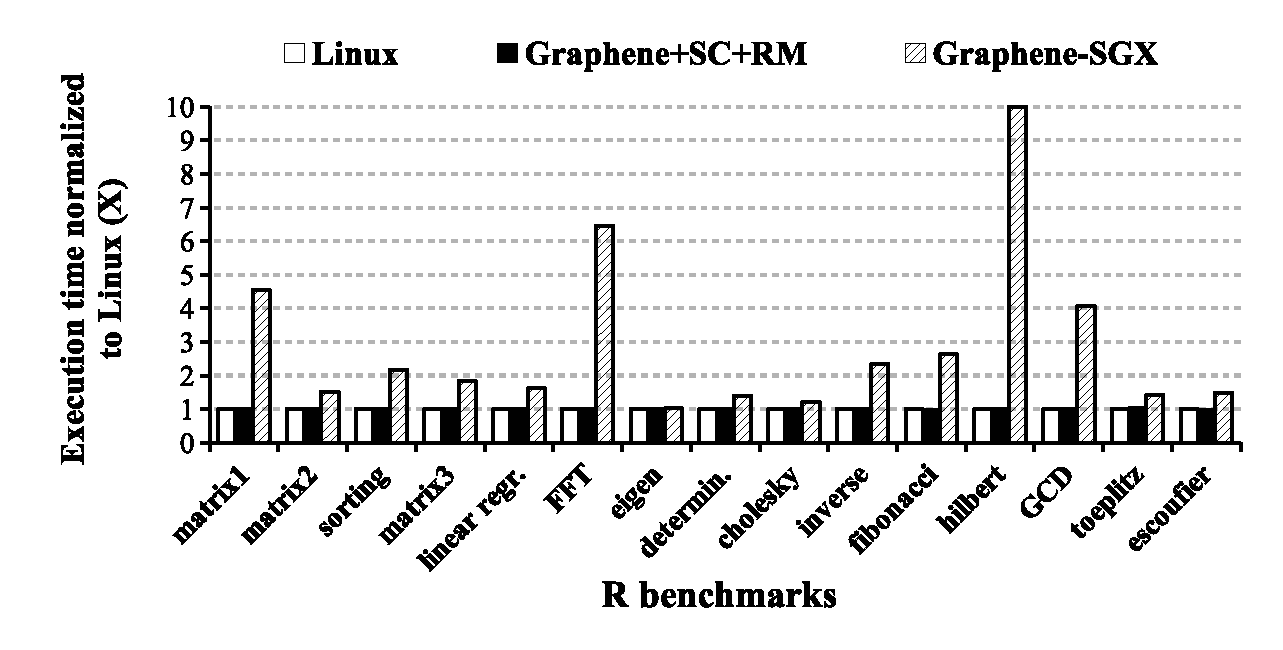
\includegraphics[width=\linewidth]{sgx/r-overhead}\\
{\bf (a) R}
\end{minipage}
\begin{minipage}{.275\textwidth}
\centering
\includegraphics[width=\linewidth]{sgx/gcc-overhead}\\
{\bf (b) GCC}
\end{minipage}
\begin{minipage}{.25\textwidth}
\centering
\includegraphics[width=\linewidth]{sgx/curl-overhead}\\
{\bf (c) CURL}
\end{minipage}

\caption{Performance overhead on desktop applications, including latency of R, execution time of GCC compilation, download time with CURL. The evaluation compares native Linux, \graphene{}, and \graphenesgx{}.} %{\bf Enclave creation time is deducted from the GCC execution time.}}
\label{fig:desktop-overhead}
\end{figure*}



\subsection{Command-Line applications}


We also evaluate the performance of a few commonly-used command-line applications.
%, to evaluate the performance of \graphenesgx{} on PCs instead of servers and clouds.
Three off-the-shelf applications are tested in our experiments:
{\bf R} (v3.2.3) for statistical computing~\cite{r-project}; {\bf GCC} (v5.4), the general GNU C compiler~\cite{gcc}; {\bf CURL} (v7.74), the default command-line web client on UNIX~\cite{curl}.
These applications are chosen because they are frequently used by Linux users,
and each of them potentially  be used 
in an enclave to handle sensitive data---either on a server or a client
machine.
% can realize profitable scenarios of using enclaves on desktop machines.



We evaluate the latency or execution time of these applications. 
%, because desktop users tend to care more about responsiveness than throughput.
In our experiments, both R and CURL have internal timing features to measure the wall time
of individual operations or executions.
%However, for other applications like GCC which does not include internal timing, evaluating the execution time can be influenced by many factors.
On a Linux host, the time to start a library OS is higher than a simple 
process, but significantly lower than booting a guest OS in a VM or
starting a container. 
Prior work measured Graphene (non-SGX) start time at 641 $\mu$s~\cite{tsai14graphene}, whereas starting an empty Linux VM takes 10.3s and starting a Linux (LXC) container takes 200 ms~\cite{agarwal15container}. 
%% dp; Note that this is MILLI seconds, not micro seconds.
%average memory footprint of an empty Linux VM, with memory deduplication, is about 96MB, . 


On SGX, the enclave creation time is relatively higher, \fixme{added more detailed number} ranging from 0.5s (a 256MB enclave) to 5s (a 2G enclave), which is a fixed cost that any application framework
will have to pay to run on SGX.
%For library OSes, the time for creating and initializing an enclave is not trivial, because it is similar to booting an lightweight OS.
% a significant part of the start-up time
% of an application is more significant, because creating enclaves is expensive.
%We consider the enclave creation time as a fixed cost for any application running in \graphenesgx{},
%and acceptable to users as long as it is responsive.
Enclave creation time is determined by the latency of the hardware and the Intel kernel driver, and is primarily a function of the size of 
the enclave, which is specified at creation time because it affects the enclave signature. %\fixmedp{although can't it grow with eadd?}.  
For non-server workloads that create multiple processes during execution,
such as GCC in Figure~\ref{fig:desktop-overhead},
the enclave creation contributes a significant portion to the execution time overheads, illustrated as a stacked bar.
%Since the enclave creation time is related to the enclave size, and unrelated to the workload,
%we deduct the enclave creation time from the execution time of GCC in Figure~\ref{fig:desktop-overhead}. \fixmedp{I think it might be better to show this as a stacked bar instead of just removing it.  Opaquely subtracting this cost doesn't seem right.  Let's discuss dp: I thought we agreed to change this...}

{\bf R}~\cite{r-project} is a scripting language often used for
data processing and statistical computation.
With enclaves, users can process sensitive data on an
OS they don't trust.
We use an R benchmark suite developed by Urbanek et al.~\cite{r-benchmark-25}, which includes 15 CPU-bound workloads such as matrix computation and number processing.
\graphenesgx{} slows down by less than 100\% on the majority of the workloads, excepts the ones which involve allocation and garbage collection: ({\tt matrix1} creates and destroys matrices, and both {\tt FFT} and {\tt hilbert} involve heavy garbage collection.)
Aside from garbage collection, these R benchmarks do not frequently interact with the host.
We further note that non-SGX \graphene{} is as efficient as Linux on all workloads, 
and these overheads appear to be SGX-specific.
%\fixmedp{Check this pontification}
In our experience, garbage collection and memory management code in managed language runtime
systems tends to be written with assumptions that do not match enclaves,
such as a large, sparse address space or that memory can be demand paged 
nearly for free (SGX version 1 requires all memory to be mapped
at creation); a useful area for future work would be to design
garbage collection strategies that are optimized for enclaves.
%we believe the overheads on \graphenesgx{} are contributed by enclaves.
 
{\bf GCC}~\cite{gcc} is a widely-used C compiler.
By supporting GCC in enclaves, developers can compile closed-source applications on customers' machines,
without leaking the source code.
GCC composes of multiple binaries, including {\tt cc1} (compiler), {\tt as} (assembler), and {\tt ld} (linker).
Therefore, GCC is a multi-process program using \syscall{execve}.
We test the compilation of thee source files with varied sizes,
using single C source files collected by MIT~\cite{gcc-benchmark}.
Each GCC execution typically \fixme{it's five, not four} creates five processes, and we run each process in a 256MB enclave by default.
%and has a fixed cost on enclave creation, which is unrelated to workload and depends on the enclave size.
%\fixme{check this}
\fixme{clarified this part, to prevent confusion between latency and overhead. also, GCC numbers got better.}
For a small workload like compiling {\tt gzip.c} (5 kLoC), running in \graphenesgx{} (4.1s) is 18.7$\times$ slower than Linux (0.2s).
The bulk of this time is spent in enclave creation, taking 3.0s in total, while the whole execution inside the enclaves, including initialization of the library OS and OS shield, takes only 1.1s, or 4.2$\times$ overhead.
For larger workloads like {\tt oggenc.c} (50 kLoC) and {\tt gcc.c} (500 kLoC), 
the overhead of \graphenesgx{} is less significant. % (3.6$\times$ and 2.1$\times$ overhead, respectively).
For {\tt gcc.c} (500 kLoC), we have to enlarge one of the enclaves ({\tt cc1}) to 2GB,
but running on \graphenesgx{} (53.1s) is only 2.1$\times$ slower than Linux (17.2s),
and 7.1s is spent on enclave creation.
%and the creation of four enclaves takes 8s.
%Each compilation has a fixed enclave creation time in \graphenesgx{}, which is about 1--2 seconds per enclave. We deduct the creation time of all enclaves  to gain more meaningful results, but do not hide rest of the overhead on fork.
%\fixmedp{Also not comfortable with this; add a bar?}
%In general, GCC in \graphenesgx{} is 1--5$\times$ slower than GCC on native Linux. 
%\fixmedp{This really needs some profiling if possible}
The overhead of non-SGX \graphene{} on GCC is marginal.
 



{\bf CURL}~\cite{curl} is a command-line  web downloader.
\graphenesgx{} can make CURL into a secure downloader that attests both server and client ends.
We evaluate the total time to download a large file, ranging from 1MB to 1GB, from another machine running Apache. % over Gigabit LAN.
%across high-speed university network\fixmedp{more specific, as above}.
\graphene{} has marginal overhead on CURL, and
\graphenesgx{} adds 7--61\% overhead to the downloading time of CURL, due to the latency of I/O.


\begin{figure*}[t!]
\centering

\begin{minipage}{.3\textwidth}
\centering
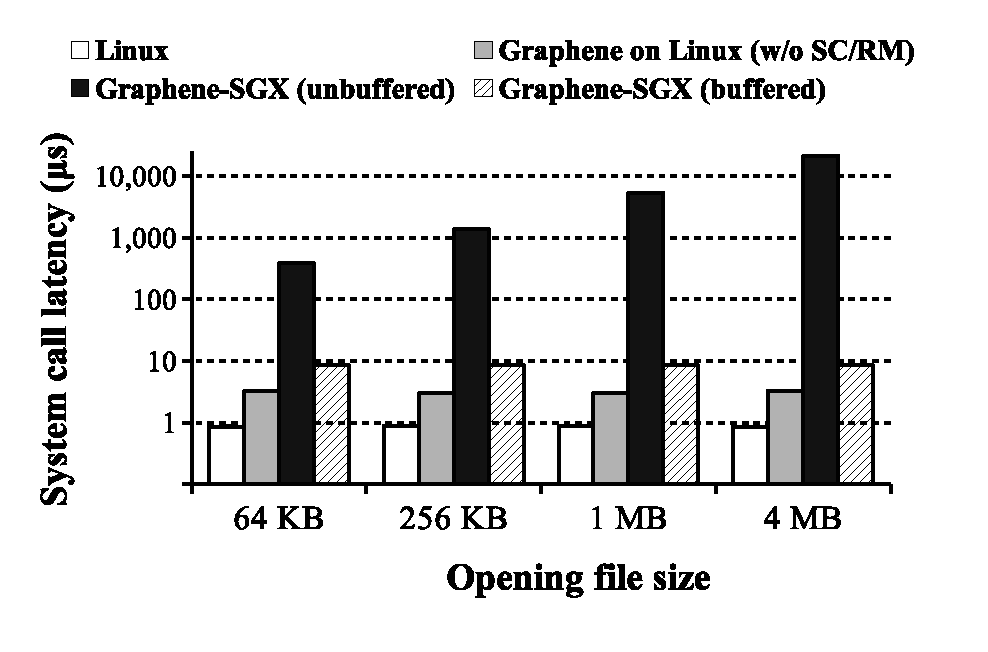
\includegraphics[width=\linewidth]{sgx/open-latency}\\
{\bf (a) Open a file}
\end{minipage}
\begin{minipage}{.3\textwidth}
\centering
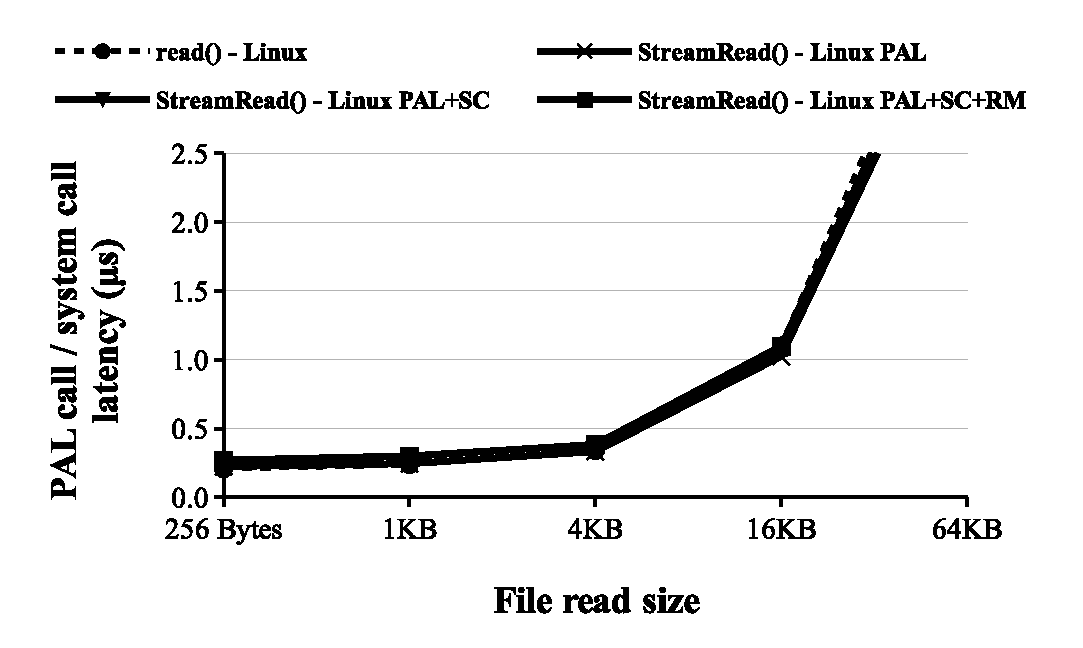
\includegraphics[width=\linewidth]{sgx/read-latency}\\
{\bf (b) Read a file}
\end{minipage}
\begin{minipage}{.3\textwidth}
\centering
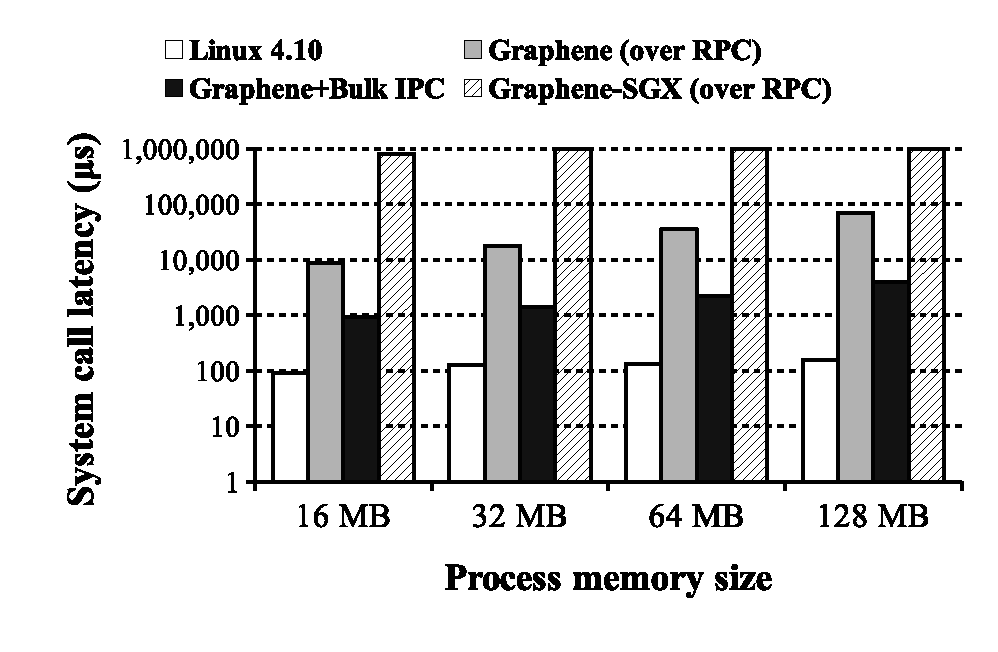
\includegraphics[width=\linewidth]{sgx/fork-latency}\\
{\bf (c) Fork a process}
\end{minipage}

\caption{Latency of some expensive system calls in \graphenesgx{}, including opening and reading a secured (authenticated) file, and forking a new process. The results are compared with native Linux and \graphene{}.}
\label{fig:syscall}
\end{figure*}


\subsection{Performance Overhead Analysis}


In this section we evaluate a few system operations that are heavily impacted by the \graphenesgx{} design.
%To shield dynamic loading and process creation,
%\graphenesgx{} uses computationally-expensive cryptographic techniques \fixmedp{more specific?} to verify enclave inputs.
% under the circumstance that the host OS cannot be trusted.
%As a trade-off to the security, the performance will be affected
%by additional cryptographic computation.
We measure the \syscall{open}, \syscall{read}, and \syscall{fork} system calls
using LMbench 2.5~\cite{McVoy:lmbench}.
A primary source of the overheads on these system calls is the cost of shielding applications, with run-time checks on the inputs.
Cryptographic techniques are used to: (1) validate the file against the secure hash, at \syscall{open}, (2) check the file chunks against the Merkle tree, at \syscall{read}, and (3) establish a TLS connection over inter-enclave RPC, at \syscall{fork}.
%opening a integrity-sensitive file for the first time, 
% or using cryptographic techniques, such as secure hashing, to verify the inputs.
% microbenchmarking specific system calls: 
% system calls,
%with different application settings.
%The microbenchmark is part of the LMBench 2.5 test suite
%\fixmedp{maybe merge this in the above paragraph, which feels a little coy}
%For instance, in order to shield dynamic loading, \graphenesgx{} checks each binary file against the secure hashes in the manifest,
%when the file is opened for the first time---after the whole file is copied into the enclave.
%\fixmedp{This happens after they are copied into enclave, memory right?}
%The verification happens when opening the file for the first time (often by the 
%After \graphenesgx{} validates the file, we generate a series of hashes of the file in chunks, as a merkle tree.
%to prevent verifying the whole file again when later randomly reading a part of the file.
%\fixmedp{So is this for the case when a file is swapped out?  I'm confused here - some details are missing}
%The latency of opening and reading an authenticated file in \graphenesgx{} is dominated by SHA256 and SHA512 calculation.
The remaining overheads contribute to exiting the enclave for host system calls, and bringing memory into the EPC (enclave page cache) or decrypting 
memory on a last-level cache miss. %and later the cache where the memory is decrypted by the CPU.


Figure~\ref{fig:syscall}(a)
shows the overhead for authenticating files in \syscall{open}.
\fixme{change overhead to latency}
Depending on the file size, the latency of \syscall{open} on \graphenesgx{} is 383$\mu$s (64KB file) to 21ms (4MB file), whereas on Linux, the latency is constant at 0.85$\mu$s.
We note that this is where enclaves are at a disadvantage, as \syscall{open} 
normally does not need to read file content; whereas here \graphenesgx{} uses \syscall{open}
as a point at which to validate file content.
For a subsequent \syscall{open}, when the Merkle tree is already generated, the overhead of simply exiting enclave for \syscall{open}, and searching the file list in the manifest, is about 9$\times$.
%\fixmedp{why?}


One might be able to optimize further for cases where only part of a file is accessed
with incremental hashing.  However, in the common case where nearly all of the file is accessed,
these costs are difficult to avoid when host file system is untrusted.
Another opportunity 
is to create the Merkle tree offline, when the manifest is created.
%\fixmedp{I think the second idea has legs...}


%This is an inevitable cost, because normal \funcname{open} on trusted OSes
%need not to access file content.
%After verifying the file, \graphenesgx{} buffers the chunk hash values, to skip whole-file verification when the file is reopened.

Figure~\ref{fig:syscall}(b)
shows the overhead for authenticating files in \syscall{read}, which 
is lower than \syscall{open}.
Since the whole file has been verified at \syscall{open}, the sequential \syscall{read} only verifies the chunks of files it is reading from untrusted memory.
%Reads from data cached in enclave memory are cheaper.  %\fixmedp{right? can we say how much cheaper?  Maybe add separate bars for both cases?}
% Therefore, \syscall{read} is actually much cheaper than \syscall{open}.
Depending on the size of blocks being read, the latency on \graphenesgx{} is 0.5$\mu$s (64-byte \syscall{read}) to 16.9$\mu$s (4KB \syscall{read}). The latency of \syscall{read} on Linux is \roughly{}0.1$\mu$s for any block size below 4KB.
If the file is not authenticated,
\graphenesgx{} only copies the file contents into the buffer, and the overhead reduces to 48\% (64-byte \syscall{read}) to 83\% (4KB \syscall{read}).
\fixmedp{Consider doing larger buffers, say up to 64k or even 4 MB}

%\fixmedp{In the legend for 7b, unsecure should be insecure}


Figure~\ref{fig:syscall}(c) shows the overhead of forking a process.
As described in \ref{sec:multiproc}, the latency of \syscall{fork} in \graphenesgx{} is affected by three factors:
creation of a new enclave, local attestation of the integrity, and duplicating the process state over an encrypted RPC stream.
Combining these factors, \syscall{fork} is one of the most expensive calls in \graphenesgx{}.
%, but at least it is supported natively on the current hardware.
The default enclave size is 256MB.
%which takes \roughly{}0.5s to create. 
Our evaluation shows that the latency of forking a process is around 0.8s (16MB process) to 2.7s (128MB process), but can be more expensive if the parent process uses more memory.
The trend matches the performance of \graphene{} without the bulk IPC optimization.
\fixmedp{If you want, some thoughts on how this might be improved in the future would be nice...  One good suggestion is recycling enclaves, or pre-forking so measurements can be done in parallel}
%Due to the overhead on \funcname{fork}, \graphenesgx{} is not suitable for fork-intensive workloads like Bash scripts
%if performance is critical.

\fixme{talk about a limitation of improving fork. check this.}
One way to further optimize \syscall{fork} is to reduce or avoid enclave creation time; one can potentially pre-launch a child enclave, and then migrate the process contents later when \syscall{fork} is called.
There might be another opportunity to improve the latency of process migration,
if copy-on-write sharing of enclave pages can be supported in future generations of SGX.
%Unfortunately, sending the process contents is difficult to avoid in \syscall{fork},
%as SGX disallows sharing enclave memory between multiple enclaves.

%\fixmedp{I assume 5.4 isn't done yet}



\subsection{TCB Size and Shielded Functionality}

In this section we measure the increase in TCB size of \graphenesgx{},
%in lines of code, 
as well as 
%compare the TCB size increased by \graphenesgx{} to an unmodified application, in lines of code, and 
the OS functionality shielded by the framework.
We compare to \scone{} and \panoply{}, using
%For SCONE and Panoply, we use 
numbers reported in their papers. 
%The conventional One generally assumes 
A smaller TCB is generally easier to review or possibly verify,
and is assumed to have fewer vulnerabilities.
%more implies lower burden for code review or formal verification, and less risk of writing exploitable code.
%For instance, Panoply argues that, because its use cases are typically smaller than 20kLoC, including both the application logic and Panoply itself, it is within the realm of future, automated verification~\cite{shinde17panoply}.

\fixmedp{Reviewer B asks for memory footprint, which isn't a bad idea}

\begin{table}
\footnotesize
\centering
\bgroup
\def\arraystretch{1.2}
\setlength{\tabcolsep}{0.5em}
\begin{tabular}{>{\raggedright\arraybackslash}p{9em}>{\raggedleft\arraybackslash\bf}p{7em}>{\raggedleft\arraybackslash}p{4.25em}>{\raggedleft\arraybackslash}p{4.25em}}
Components                    & \graphenesgx{}  & \scone{}     & \panoply{}  \\
\hline
libc (ld, libm, pthread)      &  1,292 &   88 & --      \\
                              & (glibc-2.19) & (musl)   &          \\
Library OS                    &     34 &  --      & --     \\
PAL / OS Shield               &     22 &   99 & 10  \\
\hline
Total                         &  1,348 &  187 & 10  \\
\hline
\end{tabular}
\egroup
\caption{TCB size (in thousands of lines of code) of \graphenesgx{}, \scone{}, and \panoply{}.}
\label{tab:tcb-size}
\end{table}

Table~\ref{tab:tcb-size} lists the lines of code in each components within the TCB of \graphenesgx{}, \scone{}, and \panoply{}.
By comparing the total TCB size, \graphenesgx{} is 9$\times{}$ larger than \scone{}, and 134$\times{}$ larger than \panoply{}.
However, the primary difference is the selection of libc: 
for maximum compatibility, \graphene{} uses glibc.
\scone{} uses the smaller musl libc, which lacks some features of glibc.
%it would be easy to use the smaller, and incomplete, musl libc.
%SCONE uses 
% Linux applications, \graphenesgx{} chooses to use a minimally-modified glibc, whereas SCONE uses the much more lightweight musl and 
\panoply{} excludes libc from its TCB,
% \fixmedp{what is their rationale, again? Check this}
to fit into the range of automated formal verification,
as they shield at the libc interface.
In principle, \graphene{} could easily support musl as well as glibc for applications
that do not need the additional features of glibc.
We also see the benefit of removing unused code from 
libraries, especially in an unsafe language,
similar to the approach taken in unikernels~\cite{unikernels}.
On balance, 
this choice of libc implementation is largely orthogonal to the issue
of how general-purpose the shields are.

%We argue that the choice of libc is orthogonal to the design of \graphenesgx{}; one can statically compile the applications against musl or glibc if TCB size is a concern, or given plenty of time, trim the libc functionality to bare minimum. 

If we focus on the TCB size of the library OS and the shields, 
\graphenesgx{} is 
%library OS and PAL in \graphenesgx{}, with the shielding layer of SCONE, we are 
44\% smaller than \scone{}. 
We cannot analyze the size of \scone{} because it is closed source.
%, although
%we suspect
%Although it is unclear what is in the implementation of SCONE, because it is not yet open-sourced, we believe the largest portion of their TCB contributes to the cryptography library.
\panoply{} has a smaller TCB in its shield, but within the same order of magnitude.
Panoply only shields 91 out of 256 supported POSIX functions; for context, POSIX 1003.1 defines 1,191 APIs~\cite{POSIX1003-1-2008}.
%out of 256 currently supported by \panoply{} \fixmedp{The better number is how many total functions in POSIX}.

All three of these compatibility layers or shields are within the same
order of magnitude in code size, and the differences are likely 
correlated with different ranges of supported functionality.
A recent study indicates that only order-of-magnitude differences in code
size correlate with reported CVE vulnerabilities; within the same order-of-magnitude,
the data is inconclusive that there is a meaningful difference in risk~\cite{security-metric}.
Thus, increased generality does not necessarily come with 
increased risk. % is not a clear relationship between risk 

% data only correlates
%with differences in code size when 

%Besides the choice of libc, we argue that the TCB size of a library OS or a shim shielding layer is actually correlated with the functionality that it supports or shields. Because none of the three frameworks have completely shielded the whole Linux system call table or POSIX, it is unclear how much code has to be added in the future. \graphenesgx{} also shows that one can always engineer a library OS with a small TCB, if most code is not reused from a monolithic OS kernel like Windows or Linux.
%A recent study of the CVE database also points out that having a larger TCB does not necessarily indicate more vulnerabilities, even when the difference is more than two order-of-magnitude. 



\input{apistudy}

\makeatletter
\def\input@path{{}}
\makeatother
\graphicspath{{}}
\section{Summary}



The Linux PAL successfully leverages a limited subset of Linux system calls,
to implement the whole PAL ABI for running a
full-featured \libos{}.
\Thehostabi{} separates the development of a host OS or hypervisor
from the complexity of emulating a sufficiently-compatible
Linux kernel.
The chapter shows that most calls in \thehostabi{}
can be directly translated to similar system calls on a Linux host kernel.
Only a few \hostapis{}, such as process creation and inter-thread synchronization, require additional attention for developing an efficient implementation strategy.



The Linux PAL also enforces robust security isolation
between mutually-untrusting applications,
by placing applications in separate, VM-like sandboxes.
The security isolation on a Linux host is based on system call restriction using a \seccomp{} filter, and a trusted reference monitor. % for checking resource access.
Security isolation at the host interface
restricts an untrusted application to explore vulnerable execution paths
inside a Linux kernel.
A \seccomp{} filter 
enforce a fixed, minimal system call profile, regardless of bloated dependency of an application.
The reference monitor follows
simple, white-listed manifest rules listing 
all the authorized files and network addresses of an application,
using well-known semantics
such as AppArmor~\cite{apparmor} or iptable-like firewall rules~\cite{iptablesman}.
The reference monitor can further enforce dynamic, process-specific isolation by splitting a sandbox
to run a child \picoproc{} under more restricted
resource permissions.
\graphene{} on a Linux host can serve as a sandbox framework
with a reduced attack surface
upon the host kernel.









\makeatletter
\def\input@path{{}}
\makeatother
\graphicspath{{}}

\declarecommand{\sysname}{\graphene{}}
\declarecommand{\pal}{PAL}
\declarecommand{\syscalls}{131}
\declarecommand{\palcalls}{43}
\declarecommand{\nativecalls}{50}
\declarecommand{\gipclines}{1,131}
\declarecommand{\sandboxmodlines}{888}
\declarecommand{\reflines}{3,568}
\declarecommand{\libclines}{606}
\declarecommand{\interfacenum}{41}
\declarecommand{\light}{lighttpd}
\declarecommand{\gcc}{gcc}
\declarecommand{\lmbench}{LMbench}
\declarecommand{\ab}{ApacheBench}
\declarecommand{\busy}{Bash}
\declarecommand{\skylake}{Skylake}

\chapter{Evaluation}
\label{chap:eval}
\paperchapter{Compatibility Measurement}
\label{chap:metric}

\makeatletter
\def\input@path{{metric/}}
\makeatother
\graphicspath{{metric/figures/}}

\declarecommand{\projecturl}{\url{http://oscar.cs.stonybrook.edu/api-compat-study}}
\declarecommand{\compatmetric}{weighted completeness}
\declarecommand{\Compatmetric}{Weighted completeness}
\declarecommand{\CompatMetric}{Weighted Completeness}
\declarecommand{\usagemetric}{API importance}
\declarecommand{\Usagemetric}{API importance}
\declarecommand{\UsageMetric}{API Importance}
\declarecommand{\unwusagemetric}{unweighted API importance}
\declarecommand{\Unwusagemetric}{Unweighted API importance}
\declarecommand{\UnwusageMetric}{Unweighted API Importance}
%\declarecommand{\byinst}{{\tt by-inst}}
%\declarecommand{\byvote}{{\tt by-vote}}
\declarecommand{\osversion}{Ubuntu Linux 15.04}
\declarecommand{\osdist}{Ubuntu/Debian Linux}
\declarecommand{\osarch}{x86-64}
\declarecommand{\kernelversion}{3.19}
\declarecommand{\osinstaller}{{\tt APT}}
\declarecommand{\packagenum}{30,976}
\declarecommand{\binarynum}{66,275}
\declarecommand{\execnum}{34,376}
\declarecommand{\librarynum}{31,899}
\declarecommand{\syscallnum}{320}
\declarecommand{\popsamples}{2,935,744}
%% dp: The weird typesetting for libc seems excessive
\declarecommand{\libc}{libc}
\declarecommand{\Libc}{Libc}
\declarecommand{\libpthread}{libpthread}
\declarecommand{\glibc}{GNU libc}

This chapter describes the formal definition of the \graphene{} host ABI.

\section{Basic Definitions}

The \graphene{} host ABI defines a set of {\em functions}, similar to the API of UNIX or POSIX.
The functions are directly called by the library OS, along with the arguments given either in the registers or on the stack.
A host-specific \graphene{} loader is responsible for resolving the linking, from the library OS to the host ABI.
\section{API compatibility metrics}
\label{sec:metric:definitions}

We started this study from a research perspective, in search of a better way to evaluate
the completeness of system prototypes with a Unix compatibility layer.
In general, compatibility is treated as a binary property
(e.g., bug-for-bug compatibility), which loses 
important information when evaluating a prototype that is almost certainly incomplete.
Papers often appeal to noisy indicators that the prototype probably covers all important use cases,
such as the number of total supported system or library calls, as well as the variety
of supported applications.


These metrics are easy to quantify, but problematic.
Simply put, not all APIs are equally important: some are indispensable (e.g., \syscall{read} and \syscall{write}),
whereas others are very rarely used (e.g., \syscall{preadv} and \syscall{delete\_module}).
A simple count of system calls is easily skewed by 
system calls that are variations on a theme (e.g., \syscall{setuid}, \syscall{seteuid}, and \syscall{setresuid}).
Moreover, some system calls, such as \syscall{ioctl},
export widely varying operations---some used by 
by {\em all} applications and many that are essentially never used (\S\ref{sec:study:opcodes}).
%We use the term {\em vectored system call} for calls, such as {\tt ioctl},
%which essentially export a nested system call table, selected by an opcode argument.
%by {\em any} applications in Ubuntu 
Thus, a system with ``partial support'' for \syscall{ioctl}
is just as likely to support all or none of the Linux applications distributed with Ubuntu.



%This paper considers system APIs (``APIs'') broadly:
%this includes system calls, as well as any other means by which OS kernel functionality is
%requested, such as a pseudo-file system ({\tt /proc}).
%This paper also considers
%libraries like libc, which are typically responsible for exporting an API, like POSIX,
%as well as the primary way application developers interact with the OS kernel.
%For applications, system libraries are also system APIs. Modern applications rarely use the kernel interfaces like system calls directly, but instead call library APIs as wrapper or translation layer of kernel interfaces. 
%For Linux platforms, \libc{}, or {\em Standard Library C}, is the most ubiquitously used system libraries, providing a large fraction of
%general-purpose APIs commonly used by every application.


%%%  for the rest of the paper) as channels upon which
%%% applications request system functionalities,
%%% based on the contract between users and OS developers.
%%% The basic form of APIs on UNIX platforms is the system call,
%%% but others exist.
%%% For example, other APIs can be used through accessing system pseudo files or devices,
%%% such as {\tt /proc} files,
%%% or even communicating with administrative services using specific protocols (not covered in this paper).
%%% Although a API can contain multiple channels ---
%%% for instance, {\tt stat} system call provides several file attributes, or a pseudo file can be either read or written ---
%%% we group the usage data by system call numbers, vectored system call operation codes, and file paths,
%%% as the basic granularities of our analysis.  



%and easy to miss important cases in single system calls with a wide variety of options, such as {\tt ioctl}.

One of the ways to understand the importance of a given interface
is to measure its impact on end-users.  
In other words, if a given interface were not supported, how many users would notice its absence?
Or, if a prototype added a given interface, how many more users would be able to use the system?
%% probably don't need this note to Bianca
%\note{Drop footnote here.}
%\footnote{This assumes that the prototype is well-supported by the developers, and the maintainers have reasonable
%  installation instructions, are responsive to bug reports, etc.  The issues around maturity and support
%  of research prototypes are orthogonal to the question of which APIs need to be present
%  in a proof-of-concept system.}
To answer these questions, we must consider both the 
difference in API usage
among applications,
and the popularity of applications among end-users.
We measure the former by analyzing application binaries,
and determine the latter from installation statistics collected
by Debian and Ubuntu~\citep{ubuntu-popularity,debian-popularity}.
An {\bf installation} is a single system installation, and can 
be a physical machine, a virtual machine, a partition in a multi-boot system,
or a chroot environment created by {\tt debootstrap}.
Our data is drawn from over 2.9 million installations
(2,745,304 Ubuntu and 187,795 Debian).
%\fixmedp{Add a summary about how big this data set is (i.e., millions of systems)}
%Although difficult to measure directly, we approximate this based on package installation statistics~\citep{ubuntu-popularity}.


%%% This paper borrows the notion of installations from the package installation statistics.
%%% An {\em installation} represents a set of software installed in a standalone environment
%%% using the provided Ubuntu or Debian package installer.
%%% An installation does not necessarily represent a physical machine;
%%% it can be a partition in a multi-boot system,
%%% a virtual machine,
%%% or even a subsystem installed by 

We introduce two new metrics: one for each API, and one for a whole system.
For each API, we measure how disruptive its absence
would be to applications and end users---a metric we call {\bf  \usagemetric{}}.
For a system, we compute a weighted percentage we call {\bf \compatmetric{}}. 
For simplicity, we define a {\bf system} as a set of implemented or translated APIs,
and assume an 
application will work on a target system if the application's API footprint is implemented on the system.
These metrics can be applied to all system APIs,
or a subset of APIs,
such as system calls 
or standard library functions.
%pseudo-file system interfaces ({\tt /proc}),
%device interfaces ({\tt /dev}), or standard library functions.
%These metrics , and is fully generalizable to other families of OS distributions.



This paper focuses on \osdist{}, as it is a well-managed Linux distribution with a wide array of 
supported software, which also collects
package installation statistics.
The default package installer on \osdist{} is \osinstaller{}.
A {\bf package} is the smallest granularity of installation, typically
matching a common library or application.
A package may include
multiple executables, libraries, and configuration files.
Packages also track dependencies, such as a package containing 
Python scripts depending on the Python interpreter.
%Note that a package may install multiple executables,
%but the granularity of a package
%typically matches a single application or a set of 
%common, supporting libraries.
%one or more application binaries, but installation statistics are only collected
%at package granularity.
\osdist{} installation statistics are collected at package granularity
and collect several types of statistics.
This study is based on
data of how many
Ubuntu or Debian installations
installed a given target package.
%Other installation statistics are ignored,
%because they do not provide complete information about users' actual choices of packages.}
%\byinst{} shows how many systems installed the package,
%and \byvote{} shows how many systems regularly use the package.
%We calculate our measurements based on both data, depending on
%whether one is interested in supporting
%{\it all} packages installed on a system, or prioritizing {\it important} packages.

%%% For a system, a package is the smallest unit of installation.
%%% %by the package installer.
%%% Each package is a set of files that will be placed into the
%%% file systems. %when the package is installed.
%%% Note that a package does not always include standalone executables.
%%% Other files that can be found in a package
%%% includes scripts, shared libraries, configuration files,
%%% or even kernel extensions (modules).
%%% For those packages that do not include executables,
%%% our study tracks their dependencies. %of those packages.
%%% For example, a package containing Python scripts will depend on
%%% the Python package.
%%% We mark both packages as compatible if Python itself is supported.



For each binary in a package---either as a standalone executable or shared 
library---we use static analysis to identify all possible APIs the binary could call,
or the {\bf API footprint}.
The APIs can be called from the binaries directly,
or indirectly through calling functions exported by other shared libraries.
A package's API footprint is the union of the API 
footprints of each of its standalone executables.
We weight the API footprint of each package by its installation frequency
to approximate the overall importance of each API.
%Based on installation statistics of the package, we approximate the transitive importance of the system calls in each binary's footprint.
Although our initial focus was on evaluating research,
our resulting metric and data analysis provide insights for
the larger community, such as trends in API usage.



% Bug-for-bug compatibility beyond our scope; techniques largely orthogonal to this study; we assume that, once a given system call (say write) is supported and works for a reasonable sample of applications, handling edge cases should be straightforward engineering.  That said, for system calls 

%%% Put current metric discussion here

%% Then a subsection on approach and assumptions



\begin{comment}
API compatibility is one of most important system properties, for maintaining the availability of the whole system and decoupling the development of the OS and every applications.
For an OS of the size of Linux or Microsoft Windows, millions of softwares and subsystems are implemented on top of the platform,
counting on the API contracted to provide its services.
If a system engineer decides to change the API,
an inevitable risk is to sweep and update every existing applications accordingly, which are designed and maintained by countless third parties in the world.

Then, why would a system engineer try to change the API of an OS?
The answer is related with the procedure of developing an OS.
When an OS prototype is built, developers have to rely on experiences and instincts to make educated guess about what to be the ideal API of the system.
As time goes by, the OS gains a larger user base, and receives feedbacks about how the API should really be designed.
As soon as a developer realizes that refining the API can effectively improve either efficiency, robustness, security or user-friendliness of the system,
the risk of losing compatibility {\em slightly} can be totally worthy.

Unfortunately, the reality is that system engineers are frighten by the cost of refining the API for being unable to know how compatibility can be effected.
Since there is no data set about the actual usage of the API among applications, they must assume any application developers can potentially depend on the API.
It often takes a very long time, says 6 years \fixmetsai{LSB took 6 years, reference?}, to confirm, announce, communicate or simply wait until the API is officially deprecated.

We argue that knowing the API usage is the first step of understanding and evaluating compatibility.
Instead of using a realistic metric, system engineers often express the affects on API compatibility by numbers of interfaces that are implemented or modified.
Evaluation by counting the interfaces is extremely inaccurate, because every part of the API have different importance among applications.
Some interfaces are simply more frequently used and thus more important than others; for example, the consequence of changing system call {\tt open}, which is used ubiquitously,  is not the same as changing others like {\tt msgget}.
\end{comment}


\begin{comment}
%Bhushan: - Begin here -
Knowing the values of system interfaces among users is the prerequisite of evaluating platform compatibility.
When OS developers test their systems, a common approach is to prepare numerous test cases that exercise individual system interfaces.
It is often a natural thing to do for OS developers to maintain a list of supported system interfaces,
for either development purpose or advertisement.
However, because system interfaces have different values for users, they cannot be equal while evaluating platform compatibility of the OS.
A frequently used system interface should be considered more important for compatibility than a rarely used one.
\end{comment}

\subsection{\Usagemetric{}}

System developers can benefit from an importance metric for APIs,
which can in turn guide optimization efforts, deprecation decisions,
and porting efforts.  
Reflecting the fact that users install and use different software packages,
%Because users install different software on different systems, 
we define
\usagemetric{} as the probability that
an API will be indispensable to 
 at least one application on a randomly selected 
installation.
We want a metric that decreases
as one identifies and removes instances
of a deprecated API,
and a metric that will remain high for an indispensable API, 
even if only one ubiquitous application uses the API.



%, the  of that API will decrease.
%Similarly, an \usagemetric{} near 100 percent indicates an API is indispensable,
%at least for one ubiquitous application.
%The unsupported API with the highest \usagemetric{} creates an upper bound on 
%the system's overall  \compatmetric{}.
%For instance, if a system is missing an API with an \usagemetric{} of 20\%,
%the \compatmetric{} will never be higher than 80\% (but could be significantly lower).


%%% Given a complete list of installed applications in an OS installation,
%%% by examining the API footprint of every application,
%%% we can easily determine whether removing an API is disruptive for such an installation.
%%% %The result is a binary property: whether the API is important to
%%% %the installation or not.
%%% However, it is hard to predict what applications an installation will include.
%%% Thus, we define the metric for API usage as the probability
%%% that that target API
%%% is indispensable for an random installation.

%\vspace{0.1in}
%{\noindent
%\fbox{\begin{minipage}{\linewidth}
%\setlength{\parindent}{-0.1in}
%\setlength{\leftskip}{0.1in}
%\setlength{\rightskip}{0.1in}
% Definition: {\bf \UsageMetric{}.} \\
%For a given API, the probability that an installation includes
%at least one application requiring the given API.
%at least one broken application
%(whose API footprint covers the target API),
%if the target API was removed.
%\end{minipage}}}
%\vspace{0.1in}

\noindent Intuitively, if an API is used by no packages or installations,
the \usagemetric{} will be {\em zero}, causing no negative effects if removed.
We assume all packages installed in an OS installation are indispensable.
As long as an API is used by at least one package,
the API is considered {\it important} for the installation.
Appendix \ref{sec:defs:usagemetric} includes a formal definition of \usagemetric{}.
 
%% Besides the metric, the popularity of system interfaces can be important development hints as well.
%% Knowing the most and least valuable system interfaces of an OS,
%% the developers can make better decision on prioritizing the maintenance or retirement of the interfaces.
%% More influences of system interface popularity are discussed in \fixmetsai{later section?}.

%We define the popularity of a system interface by the probability that an installation become unsupported if the interface is removed.
%In other word, the popularity indicates the {\em cost} or {\em penalty} of deprecating an interface.

\begin{comment}
\paragraph{Formal Definition.}
A given system installation ($\mathtt{Inst}$)
is a set of packages installed ($\{\mathtt{pkg}_1, \mathtt{pkg}_2, ..., \mathtt{pkg}_k \in \mathtt{Pkg}_\mathtt{all}\}$).
For each package $\mathtt{pkg}$ in the \osdist{} repository,
our framework generates the API footprint as 
${\mathtt{Footprint}}_\mathtt{pkg} = \{\mathtt{api}_1, \mathtt{api}_2, ..., \mathtt{api}_k \in \mathtt{API}_\mathtt{all}\}$.  
For an API supported by the OS, we calculate the \usagemetric{} as the product 
of probabilities that an installed package will require this API.
This is calculated as follows:
\begin{align*}
&\mathtt{Dependent}_\mathtt{api} = \{\mathtt{pkg}|\mathtt{api} \in \mathtt{Footprint}_\mathtt{pkg}\} \\
&\mathtt{Importance}(\mathtt{api}) = Pr\{\mathtt{Dependent}_\mathtt{api} \bigcap \mathtt{Inst} \neq \emptyset\} \\
&= 1 - Pr\{\forall \mathtt{pkg} \in \mathtt{Dependent}_\mathtt{api}, \mathtt{pkg} \notin \mathtt{Inst}\} \\
&= 1 - \prod_{\mathtt{pkg} \in \mathtt{Dependent}_\mathtt{api}} Pr\{\mathtt{pkg} \notin \mathtt{Inst}\} \\
&= 1 - \prod_{\mathtt{pkg} \in \mathtt{Dependent}_\mathtt{api}} (1 - \frac{\text{installation of $\mathtt{pkg}$}}{\text{total installation}})
\end{align*}
\end{comment}


\subsection{\Compatmetric{}}

We also measure compatibility at the granularity of an OS,
which we call \compatmetric{}.
\Compatmetric{} is the fraction of applications that are likely to work,
weighted by the likelihood that these applications will be installed on a system.
%\fixmedp{check this synopsis}
% function of the APIs supported, weighted by the popularity 
%of the applications that require these APIs.

The goal of \compatmetric{} is to measure the degree to which a
new OS prototype or translation layer is compatible with a baseline OS.
In this study, the baseline OS is \osdist{}.



%%  as a function of the API footprint of each potentially-installed
%% application, weighted by the popularity of each application.
%% We introduce the metric , which we define in terms of an OS installation (i.e.,
%% the libraries and applications) and a target API implementation, which may provide a subset
%% of the original system's APIs.


%% An accurate metric for API compatibility must take into account at least two factors:
%% \begin{compactenum}
%% \item For each interface in the API, what are the applications that rely on it and could be affected if the interface is removed? ({\em application footprint})
%% \item For each application, how many installations of the system in the world has included it? ({\em application popularity})
%% \end{compactenum}


%% \fixmedp{Term for each call, vs system overall: API Importance and Effective Coverage?}

%% To accurately evaluate compatibility, we design a metric that is quantifiable, \fixmetsai{one more word here}, and easy to interpret.

\begin{comment}
We defined {\bf platform compatibility} as "{\em the probability of porting any installation of an OS distribution onto the target OS without any effort}".
The definition of an {\em installation} is a combination of application setup on a standalone OS instance.
An Installation can exist on physical machines,
or any machines of generalized sense such as a virtual machines, containers or subsystems.
In our model, installations represent customers of the OS, who are considered equal when providing any services.
\end{comment}

%\vspace{0.1in}
%\fixmetsai{Find a good name for our metric} 
%{\noindent
%\fbox{\begin{minipage}{\linewidth}
%\setlength{\parindent}{-0.1in}
%\setlength{\leftskip}{0.1in}
%\setlength{\rightskip}{0.1in}
%Definition: {\bf \CompatMetric{}.} \\
%For a target system, the fraction of applications supported,
%weighted by the popularity of these applications.
%For any installation, the expected fraction of installed applications that can work on the target OS.
%\fixmedp{shouldn't the weight go in the definition?}
%\Compatmetric{} is the total size of all supported applications,
%weighted by the popularity of each application.
%\end{minipage}}}
%\vspace{0.1in}

%\noindent In terms of porting effort, we are primarily interested in avoiding code changes, 
%such as {\tt \#ifdef LINUX}; although we leave this notion somewhat vague.
%We consider recompilation, relinking, or other mechanical processes acceptable.

%% Our analysis framework scans through all available packages in the \osdist{} repository and generates system interface footprint data for individual package.
%% The footprint data is based on static analysis,
%% and it lists all potentially used system interfaces regardless of the applications' runtime coverage. 
%% To build the metric, we also import the package popularity statistics from the official \osdist{} reports~\citep{ubuntu-popularity, debian-popularity}.

The methodology for measuring the \compatmetric{} of a target system's API subset is summarized as follows:
\begin{compactenum}
\item Start with a list of supported APIs of the target system, either identified from the system's source, or as provided by the developers of the system.
\item Based on the API footprints of packages, the framework generates a list of supported and unsupported packages.
\item The framework then considers the dependencies of packages. If a supported package depends on an unsupported package, both packages are marked as unsupported.
\item Finally, the framework weighs the list of supported packages based on package installation statistics.
As with \usagemetric{}, we measure the effected package that is most installed;
\compatmetric{} instead calculates the expected fraction of packages in a typical installation that will work on the target system.
%Specifically, each package's weight is based on 
%and the framework calculates the expected fraction of packages from a typical installation that will work on the target system.
\end{compactenum}
%\fixmedp{``typical installation'' raised some hackles.  Can we either use a different term, or talk more about this concept?}

\begin{comment}
\paragraph{Formal Definition.}
Suppose an OS supports a set of APIs ($\mathtt{API}_\mathtt{Supported}$),
% = \{i_1, i_2, ..., i_n\}$
which is a subset of the APIs of the original system ($\mathtt{API}_\mathtt{all}$).
In this study, $\mathtt{API}_\mathtt{all}$ is the sum of Linux APIs, including
the system call table, sysctl, proc, and so forth.
%(total APIs are $\Sigma = \{i_1, i_2, ..., i_m\}, m \geq n$).
A list of supported packages ($\mathtt{Pkg}_\mathtt{Supported}$) can be generated by checking whether the API footprint is
a subset of the target system's supported APIs ($\mathtt{API}_\mathtt{Supported}$):
\begin{align*}
\mathtt{Pkg}_\mathtt{Supported} = \{\mathtt{pkg} | \mathtt{Footprint}_\mathtt{pkg} \subseteq \mathtt{API}_\mathtt{Supported}\}
\end{align*}
\end{comment}


\vspace{10pt}
We note that this model of a typical installation is useful in reducing the metric to a single number,
but also does not capture the distribution of installations.
This limitation is the result of the available package installation statistics,
which do not include correlations among installed packages.
%Using package installation statistics has the important limitation that 
%which package installations are correlated.
This limitation requires us to 
assume that package installations are independent,
except when \osinstaller{} identifies a dependency.
For example, if packages {\em foo} and {\em bar} are both reported as being installed once,
we cannot tell if they were on the same installation, or if two different installations.
If foo and bar both use an obscure system API, we assume that two installations would be affected if the obscure API were removed.
If foo depends on bar, we assume the installations overlap. % overlapping installations are on the same system.
%We note that packages do include installation dependences, which could be used in future work to reduce this over-approximation.
%\fixmedp{Check my edit: I was confused by the old wording}
Appendix \ref{sec:defs:compatmetric} formally defines \compatmetric{}.



%% In our experiment, we assume installation of any packages to be {\em independent events}.
%% This is a strong assumption that can affect the precision of the metric.
%%  We introduce the assumption for the following reasons:
 
%%  \begin{compactenum}
%%  \item The official \osdist{} package popularity reports contain no relative popularity between packages. Neither is the raw data of individual installation published. 
%%  \item Most of the packages depend on others due to library dependency. Our analysis combines the popularity among libraries into the statistics of executables, and only counts executables for evaluation. 
%%  \end{compactenum}
 
%% As a limitation, we do not consider the case where executables may have relative popularity due to users' preference. For example, Apache-PHP-Mysql is a combination installed on many machines that provide web services.
%% In our experiment, we assume installation of each package is irrelevant with others.

\begin{comment}
Formally, \compatmetric{} is the expected fraction of packages on a given system($\mathtt{Inst}$)
having an API footprint within the target 
system's supported APIs.
%We approximate the expected value as follows:
%Based on the list of supported packages, we can calculate the probability of an installation $\zeta = \{p^{\zeta}_1, p^{\zeta}_1, ..., p^{\zeta}_q\}$ to be fully compatible as follows:
By assuming independence of package installation, we can calculate the probability of supporting an installation as follows:
\begin{align*}
&\mathtt{Weighted Compliance}(\mathtt{API}_\mathtt{Supported}) =\\
&E(\frac{|\mathtt{Pkg}_\mathtt{Supported} \bigcap \mathtt{Inst}|}{|\mathtt{Inst}|}) \sim \frac{E(|\mathtt{Pkg}_\mathtt{Supported} \bigcap \mathtt{Inst}|)}{E(|\mathtt{Inst}|)} \\
&\sim \frac{\sum_{\mathtt{pkg} \in \mathtt{Pkg}_\mathtt{Supported}} (\frac{\text{installation of $\mathtt{pkg}$}}{\text{total installation}})}{\sum_{\mathtt{pkg} \in \mathtt{Pkg}_\mathtt{all\hspace{0.21in}}} (\frac{\text{installation of $\mathtt{pkg}$}}{\text{total installation}})} \\
&\text{where E}(\mathtt{x})\text{ is the Expectation of }\mathtt{x}\text{ occurring.}
\end{align*}
\end{comment}

%% dp:Meh
%\subsection{Justifying the Practicability of the Metric}

\section{Data collection}
\label{sec:metric:collection}

We use static binary analysis to identify the system call footprint of a binary.  This approach has the advantages
of not requiring source code or test cases.  Dynamic system call logging using a tool like {\tt strace} is simpler,
but can miss input-dependent behavior.  A limitation of our static analysis is that we must assume the disassembled binary
matches the expected instruction stream at runtime.  In other words, we assume that the binary isn't deliberately obfuscating
itself, such as by jumping into the middle of an instruction (from the perspective of the disassembler).
%In practice, such obfuscation is generally done only by malware, and our results are not concerned with system security.
To mitigate this, we spot check that static analysis returns as superset of {\tt strace} results.

We note that, in our experience, things like the system call number or even operation codes are fairly straightforward
to identify from a binary.  These tend to be fixed scalars in the binary, whereas other arguments, such as the contents of a write buffer,
are input at runtime.
We assume that binaries can issue system calls directly with inline system call instructions, or can call system calls through a library, such as \libc{}.
Our static analysis identifies system call instructions and constructs a whole-program call graph.

\begin{figure}[t!]
\centering
\includegraphics[width=3.2in]{executable-type.pdf}\includegraphics[width=2.4in]{elf-binary-type.pdf}
\vspace{-0.5in}
\footnotesize
\caption{Percentage of ELF binaries and applications written in interpreted languages among all executables in the \osdist{} repository, categorized by interpreters. ELF binaries include static binaries, shared libraries and dynamically-linked executables. Interpreters are detected by {\em shebangs} of the files. Higher is more important.}
\label{fig:syspop:executable-type}
\end{figure}

Our study focuses primarily on ELF binaries, which account for the largest fraction of Linux applications
%which account for the plurality of Linux applications
(Figure~\ref{fig:syspop:executable-type}).
For interpreted languages, such as Python or shell scripts,
we assume that the system call footprint of the interpreter and major supporting libraries over-approximates the expected system call footprint of the applications.
Libraries that are dynamically loaded, such as application modules or
language native interface (e.g.,JNI, Perl XS) are not considered in our study. 
%\fixmedp{Does the analysis handle JNI, Perl XS, or other wrappers for native libraries?  I 
%could imagine the answer being yes if a .so is shipped, but possibly no 
%if it is somehow inlined}

%\fixmedp{Maybe move this up and merge with discussion above}

%% Similarly, there is a distinction between installation and regular use.  Ideally, one might filter applications
%% that were installed but never used, or have a second variant of \usagemetric{} that is weighted by frequency of use.
%% %Although we leave this for future work
%% However, we hasten to note that some infrequently-used applications are nonetheless important to users,
%% and frequency-independent metrics are still important.
%Similarly, there is a distinction between installation and regular use.
%Figure~\ref{fig:package-popularity} shows the trend of package installation statistics for the 500 most commonly installed packages.
%The \byinst{} data may {\it over-approximate} the \usagemetric{} of a package,
%whereas the \byvote{} may {\it under-approximate} important, but infrequently used packages.
%We err on the side of over-approximating \usagemetric{}, using \byinst{}
%weighting where not otherwise specified,
%although we present measurements based on both when appropriate.
%instead under-approximating is a safer strategy to quarantee the compatibility requirements to be fully deliverable.
%In this paper, we present measurements based on both \byinst{} and \byvote{} statisitcs to draw more observations.

%\begin{figure}[t!]
%\vspace{-0.1in}
%\center{
%\includegraphics[width=3.6in]{figures/package-popularity.pdf}
%}
%\footnotesize
%\vspace{-10pt}
%\caption{Package installation statisitics in \osdist{}, for 500 most installed packages managed by the repository. \byinst{} shows installations of packages. \byvote{} shows regularly used packages voted by installations. Higher is more popular.\fixmebj{Change the scale.}}
%\label{fig:package-popularity}
%\end{figure}


\section{Implementation Details}
\label{sec:framework}

This section provides additional implementation details of our analysis framework. % for mining the API footprint for ELF executables and libraries.

%Analyzing the footprint of an applications requires interpretation of its behavior. As discussed in section~\ref{sec:measure:analysis}, we choose to build our framework by using {\bf static analysis} technique instead of dynamic analysis. The reason is that static analysis can trace potential executions of the applications, regardless of the runtime coverage of the code.

Our analysis is based on disassembling binaries inside each application package, using the standard {\tt objdump} tool.
This approach eliminates the need for source or recompilation, and can handle closed-source binaries.
We implement a simple call-graph analysis to detect system calls reachable from the binary entry point ({\tt e\_entry} in ELF headers). 
%\fixmedp{You do actually parse the elf header for e\_entry, right?}
%In our study, we only count executables during measuring both \usagemetric{} and \compatmetric{}.
We search all binaries, including libraries, for system call instructions ({\tt int \$0x80}, {\tt syscall} or {\tt sysenter}) or calling the {\tt syscall} API of \libc{}.
We find that the majority of binaries --- either shared libraries or executables --- do not directly choose system calls, but 
rather use the GNU C library APIs.
Among 66,275 studied binaries, only 7,259 executables and 2,752 shared libraries issue system calls.

% system calls. Therefore, analyzing the libraries that an executable depends on is necessary for retrieving a complete set of API footprint.


%, to predict its runtime behaviors.
%The framework requires no scanning of the source code, or recompiling of the applications with additional debug symbols.
%Consider the size and complexity of Ubuntu repositories,
%static analysis of ELF binaries is certainly easier to automate, and is able to analyze the applications that are close-sourced.

%To trace the footprint of applications, it require {\em Call-Graph Analysis} to rip off potential control flows that can eventually lead to usage of system API.
%Challenges of analyzing call-graph is a known issues for researchers in many area such as security, robustness, etc.

Our call-graph analysis allows us to only select system calls that are actually used by the application, not all the system calls that appear in \libc{}.
Our analysis takes the following steps:
\begin{compactitem}
\item For a target executable or a library, generate a call graph of internal function usage.
\item For each library function that the executable relies on, identify the code in the library that is reachable from each entry point called by the executable.
%trace coverage of code in the binary, and generate the minimal subset of the library's footprint that the function could actually link to.
\item For each library function that calls another library call, recursively trace the call graph and aggregate the results. 
\end{compactitem}
\vspace{10pt}

Precisely determining all possible call-graphs from static analysis is challenging.
Unlike other tools built on 
call-graphs, such as control flow integrity (CFI), our framework can tolerate the error caused by over-approximating the analysis results.
For instance, 
programs sometimes make function call based on a function pointer passed as an argument by the caller of the function. 
Because the calling target is dynamic, it is difficult to determine at the  call site.
Rather, we track sites where the function pointers are assigned to a register, such as using the {\tt lea} instruction with an address
relative to the current program counter.
%Instead of precisely tracking calling target at the {\tt call} instruction, 
%A function pointer is mostly assigned by {\tt lea} instruction to generate a relative address to the current program counter. 
This is an over-approximation because, rather than trace the data flow, we assuming that a function pointer assigned to a local variable will be called.
This analysis could be more precise if it included a data flow component. 
%\fixmedp{As an aside, this level of data flow analysis shouldn't be that hard, right?  Not  that it matters, except for the thesis/journal version.}

We also hard-code for a few common and problematic patterns.
For instance, we generally assume that the registers that pass a system call number to a system call,
or an opcode to a vectored system call, are not the result of arithmetic in the same function.
We spot checked this assumption, but did not do the data flow analysis to detect this case.

%must trace the register values such as {\tt RAX/EAX} for system call number or {\tt RBX/EBX} for parameter to vectored system calls. 

%Based on {\em Case-by-case study}, we assume no arithmetic but direct assignment of integers is possible when the program is issuing a system call. 

%If our analysis cannot precisely determine whether an API is used, we 
%err on the side of assuming an API is used.

%In the case of a run

%allow slightly enlarge the traced footprint of application, to gain simplicity for complex call-graph analysis corner cases. 
%For the specific run-time scenario of the application that can hard to interpret, we do a {\bf Case-by-Case study} to find out strategy of analyze the footprint practicably.

%  that call-graph analysis is complex for generating the accurate control flow of the run time. Fortunately, unlike other studies that relies on 

%In our study, we specifically call it {\bf Over-approximation}. 


%The following is a few example of using {\bf Over-approximation} and {\bf Case-by-Case study} to simplify call-graph analysis:
%\begin{compactenum}
%\item 
%\item 
%\end{compactenum}

Finally, the last mile of the analysis is to recursively aggregate footprint data. We insert all raw data into a {\tt Postgresql} database, and 
use recursive SQL queries to generate the results. 
To scan through all \packagenum{} packages in the repository, collect the data, and generate the results takes roughly three days.

   




\declarecommand{\sysname}{\graphene{}}
\declarecommand{\pal}{PAL}
\declarecommand{\syscalls}{131}
\declarecommand{\palcalls}{43}
\declarecommand{\nativecalls}{50}
\declarecommand{\gipclines}{1,131}
\declarecommand{\sandboxmodlines}{888}
\declarecommand{\reflines}{3,568}
\declarecommand{\libclines}{606}
\declarecommand{\interfacenum}{41}
\declarecommand{\light}{lighttpd}
\declarecommand{\gcc}{gcc}
\declarecommand{\lmbench}{LMbench}
\declarecommand{\ab}{ApacheBench}
\declarecommand{\busy}{Bash}
\declarecommand{\skylake}{Skylake}

\chapter{Evaluation}
\label{chap:eval}

\subsection{Limitations}
\label{sec:metric:limitations}

%\fixmedp{Make sure we explain these:  the fact that the new metrics cannot distinguish between APIs that are critical to a small population, in that their functionality cannot be provided any other way, because they are new APIs not yet widely adopted, or because they are old APIs that are no longer used or were never used.}

\paragraph{Popularity Contest Dataset.}
The analysis in this paper is limited
by the \osdist{}'s package installer, \osinstaller{},
and their package installation statistics.
Because most packages in \osdist{} are open-source,
our observations on Linux API usage may have a bias toward open-source development patterns.
Commercial applications that are purchased and distributed
through other means are not included in this survey data,
although data from other sources could, in principle, be incorporated
into the analysis if additional data were available.
%the analysis can only be conducted manually,
%thus making it really hard to collect large amounts of samples.

We assume that the package installation statistics provided by \osdist{} are representative.
%The \osdist{} repository hosts \packagenum{} packages that contain application executables and libaries. 
The popularity contest dataset is reasonably large (\popsamples{} installations),
but reporting is opt-in.
Moreover,
%\fixmedp{check this para}
%The popularity contest dataset does not correlate 
%package installations, only shows how often each package is installed.
%Thus, we assume the installation of every package
%as an independent event, unless \osinstaller{} identifies the dependency otherwise.
the data does not show how often these packages
are actually used, only how often they are installed.
Finally, this data set does not include sufficient historical data
to compare changes to the API usage over time.


%% Another limitation of using
%% the package installation statistics
%% is that the statistics only show
%% the installation count of each package,
%% but no details about which packages each installation contains or
%% relative preferences among packages.
%% Therefore, our study must 




%% dp: This is covered elsehwere
%The usage statistics collected in this paper generate
%convincing observations and measurements for Linux-compatible platforms,
%due to the large-scale analysis of software packages in the \osdist{} repository.
%Although our analysis does not require source code,
%our resulting dataset is mostly focused on open-source applications.
%Only very few applications in the \osdist{} repositories are close-source,
%such as the Nvidia driver utilities.
%Our analysis only requires application binaries, and our resulting dataset covers 
%both open-source and closed-source applications. \fixmedp{Right?  Double check that do include some closed binaries}
%Because we focus on \osdist{} applications, and most are open-source (xx\% \fixmetsai{Need to find this number, it's not hard.}),
%the data may be biased toward open-source applications. 
%As a result, our observations on Linux API usage are largely biased toward open-source applications.
%Because the repositories for close-source applications
%are more scattered
%(even though they can be downloaded by \osinstaller{} if manually configured),
%it is hard to collect large amount samples about them.

%% Our study is focused on applications managed by \osinstaller{},
%% which are mostly open-source
%% (even though our approach requires no source code for analysis).

\paragraph{Static Analysis.}
Because our study only analyzes pre-compiled binaries, some compile-time customizations may be missed.
Applications that are already ported using macro like {\tt \#ifdef LINUX} will be considered dependent to Linux-specific APIs,
even though the application can be re-compiled for other systems.
Our static analysis tool only identifies 
whether an API is potentially used,
not how frequently the API is used during the execution.
Thus, it is not sufficient to draw inferences about performance.

%This study is only sufficient to draw conclusions or insight about compatibility, not about any impact on performance.
%The static analysis on application binaries only tells
%Also the package installation statistics provide no information
%about how often a package is used.
%This study cannot provide evidence for whether any APIs may dominate
%execution time.


%\note{Move this here}
We assume that, once a given API (e.g., {\tt write}) is supported and works for a reasonable sample of applications,
handling missed edge cases should be straightforward engineering that is unlikely to invalidate the experimental results of the project.
That said, in cases where an input can yield significantly different behavior, e.g.,
the path given to {\tt open},
we measure the \usagemetric{} of these arguments.
Verifying bug-for-bug compatibility generally requires techniques largely orthogonal to the ones used in this study,
and thus this is beyond the scope of this work.

We do not do inter-procedural data-flow analysis.  As a result,
we were unable to identify system call numbers for 2,454 call sites (4\% of the
relevant call sites)
across all binaries in the repository.  As a result,
some system call usage values may be underestimated, and may go up 
with a more sophisticated static analysis.


%% The package installation statistics provided by \osdist{}
%% show only information about how often packages are ``installed'',
%% not how often packages are ``used''.
%% Our study is based on an over-approximation of the actual package usage:
%% installed packages in any installation contain
%% at least the packages actually used.


\paragraph{Metrics.}
The proposed metrics are intended to be simple numbers for easy comparison.
But this coarseness loses some nuance. 
For instance, our metrics cannot distinguish between
APIs that are critical to a small population, such as those that offer 
functionality that cannot be provided any other way, 
versus APIs that are rarely used because the software is unimportant.
Similarly, these metrics alone cannot differentiate a new API 
that is not yet widely adopted from an old API with declining usage.


%% Although studying historical data may provide more insight about
%% how developer or user behaviors change, our approach requires more historical data to make any conclusions.
%% The installation statistics contain no version information,
%% so it is insufficient to determine the adoption time of any application changes.
%% For packages, \osinstaller{} only keeps the latest version of each package in each maintained snapshot.
%% The only way to backtrace all historical versions of a package
%% is to pull from a version-control repository maintained by the package developers, which may not always exist.

\section{Evaluating Existing Systems}

This section uses \compatmetric{} to evaluate systems or emulation layers with partial Linux compatibility.
We also evaluate several \libc{} variants for their degree of completeness against the APIs exported by \glibc{} 2.21.

\subsection{Linux systems}

\begin{table}[t]
\centering
\small
\begin{tabular}{m{.3\textwidth}>{\centering}m{.05\textwidth}>{\raggedright\arraybackslash\footnotesize}m{.4\textwidth}>{\raggedleft\arraybackslash}m{.15\textwidth}}
\toprule
Systems & \# & Suggested APIs to add & \Compatmetric{} \\
\midrule
\addlinespace
User-Mode-Linux \kernelversion{} & 284 & {\tt name\_to\_handle\_at}, {\tt iopl}, {\tt perf\_event\_open} & 93.1\% \\
\addlinespace
\hline
\addlinespace
L4Linux 4.3 & 286 & {\tt quotactl}, {\tt migrate\_pages}, {\tt kexec\_load} & 99.3\% \\
\addlinespace
\hline
\addlinespace
FreeBSD-emu 10.2 & 225 & {\tt inotify}*, {\tt splice}, {\tt umount2}, {\tt timerfd}* & 62.3\% \\
\addlinespace
\hline
\addlinespace
Graphene  & 143 & {\tt sched\_setscheduler}, {\tt sched\_setparam} & 0.42\% \\
Graphene\textsuperscript{\P} & 145 & {\tt statfs}, {\tt utimes}, {\tt getxattr}, {\tt fallocate}, {\tt eventfd2} & 21.1\% \\
\hline
\end{tabular}
\caption{\Compatmetric{} of several Linux systems or emulation layers. For each system, we manually identify the number of supported system calls (``\#''), and calculate the \compatmetric{} (``W.Comp.'') . Based on \usagemetric{}, we suggest the most important APIs to add.
(*: system call family.
\P: Graphene after adding two more system calls.) }
\label{tab:linux-compat}
\end{table}

To evaluate the \compatmetric{} of Linux systems or emulation layers,
the prerequisite is to identify the supported APIs of the target systems.
Due to the complexity of Linux APIs and system implementation,
it is hard to automate the process of identification.
However, OS developers are mostly able to maintain such a list based on the internal knowledge. 

We evaluate the \compatmetric{} of four Linux-compatible systems or emulation layers:
User-Mode-Linux~\citep{user-mode-linux}, L4Linux~\citep{hartig97mu}, FreeBSD emulation layer~\citep{freebsd-emu}, and Graphene library OS~\citep{tsai14graphene}.
For each system, we explore techniques
to help identifying the supported system calls,
based on how the system is built.
For example, User-Mode-Linux and L4Linux
are built by modifying the Linux source code,
or adding a new architecture to Linux.
These systems will define architecture-specific system call tables,
and reimplement {\tt sys\_*} functions in the Linux source
that are originally aliases to {\tt sys\_ni\_syscall}
(a function that returns {\tt -ENOSYS}). 
Other systems, like FreeBSD and Graphene,
are built from scratch,
and often maintain their own system call table structures,
where unsupported systems calls
are redirected to dummy callbacks.

%Because the evaluation is simply a proof-of-the-concept,
%we count only system calls,
%omitting other APIs such as vectored system calls and pseudo-files. 

Table~\ref{tab:linux-compat} shows \compatmetric{},
considering only system calls.
The results also identify the most important system calls
that the developers should consider adding. 
User-Mode-Linux and L4Linux both have a \compatmetric{} over 90\%,
with more than 280 system calls implemented.
FreeBSD's  \compatmetric{} is  62.3\% because it is missing some less
important system calls
such as {\tt inotify\_init} and {\tt timerfd\_create}.
Graphene's \compatmetric{} is only 0.42\%.
We observe that the primary culprit is 
scheduling control; by adding two scheduling system calls,
Graphene's \compatmetric{} would be 21.1\%.

\subsection{\Libc{} variants}

\begin{table}[t]
\center{
\small
\begin{tabular}{>{\raggedright\arraybackslash}m{.25\textwidth}>{\raggedleft\arraybackslash}m{.05\textwidth}>{\raggedright\arraybackslash\footnotesize}m{.25\textwidth}>{\raggedleft\arraybackslash}m{.15\textwidth}>{\raggedleft\arraybackslash}m{.15\textwidth}}
\toprule
\Libc{} variants & \# & Unsupported functions (samples) & {\footnotesize \Compatmetric{}} & {\footnotesize \Compatmetric{}} {\scriptsize (normalized)} \\
\midrule
\addlinespace
eglibc 2.19 & 2198 & None & 100\% & 100\% \\
\addlinespace
\hline
\addlinespace
uClibc 0.9.33 & 1867 & {\tt \_\_uflow}, {\tt \_\_overflow}  & 1.1\% & 41.9\% \\
\addlinespace
\hline
\addlinespace
musl 1.1.14 & 1890 & {\tt secure\_getenv}, {\tt random\_r} & 1.1\% & 43.2\% \\
\addlinespace
\hline
\addlinespace
dietlibc 0.33 & 962 & {\tt memalign}, {\tt stpcpy}, {\tt \_\_cxa\_finalize}  & 0\% & 0\% \\
\addlinespace
\hline
\end{tabular}
}
\caption{\Compatmetric{} of \libc{} variants. For each variant, we calculate \compatmetric{} based on symbols directly retrieved from the binaries,
and the symbols after reversing variant-specific replacement (e.g.,\funcname{printf} becomes \funcname{\_\_printf\_chk}).}
\label{tab:libc-compat}
\end{table}

This study also uses \compatmetric{} to evaluate the compatibility of several \libc{} variants --- eglibc~\citep{eglibc}, uClibc~\citep{uclibc}, musl~\citep{musl} and dietlibc~\citep{dietlibc} --- against \glibc{},
listed in Table~\ref{tab:libc-compat}.
We observe that, if simply matching exported API symbols, only eglibc is directly compatible to \glibc{}.
Both uClibc and musl have a low \compatmetric{}, because \glibc{}'s headers replace a number of APIs with safer variants at compile time, using macros.
For example, \glibc{} replaces {\tt printf} with {\tt \_\_printf\_chk}, which performs an additional check for stack overflow.
%Because these new APIs often have the same interface as the old ones,
%we assume other \libc{} variants can easily
%reverse the API replacement during symbol resolution.
After normalizing for this compile-time API replacement, both uClibc and musl are at over 40\% \compatmetric{}.
In contrast, dietlibc is still not compatible with most binaries linked against \glibc{} --- if no other approach is taken to improve its compatibility.
The reason of low \compatmetric{} is that dietlibc does not implement many ubiquitously used \glibc{} APIs such as {\tt memalign} (used by 8887 packages) and {\tt \_\_cxa\_finalize} (used by 7443 packages).

\section{Summary}



The Linux PAL successfully leverages a limited subset of Linux system calls,
to implement the whole PAL ABI for running a
full-featured \libos{}.
\Thehostabi{} separates the development of a host OS or hypervisor
from the complexity of emulating a sufficiently-compatible
Linux kernel.
The chapter shows that most calls in \thehostabi{}
can be directly translated to similar system calls on a Linux host kernel.
Only a few \hostapis{}, such as process creation and inter-thread synchronization, require additional attention for developing an efficient implementation strategy.



The Linux PAL also enforces robust security isolation
between mutually-untrusting applications,
by placing applications in separate, VM-like sandboxes.
The security isolation on a Linux host is based on system call restriction using a \seccomp{} filter, and a trusted reference monitor. % for checking resource access.
Security isolation at the host interface
restricts an untrusted application to explore vulnerable execution paths
inside a Linux kernel.
A \seccomp{} filter 
enforce a fixed, minimal system call profile, regardless of bloated dependency of an application.
The reference monitor follows
simple, white-listed manifest rules listing 
all the authorized files and network addresses of an application,
using well-known semantics
such as AppArmor~\cite{apparmor} or iptable-like firewall rules~\cite{iptablesman}.
The reference monitor can further enforce dynamic, process-specific isolation by splitting a sandbox
to run a child \picoproc{} under more restricted
resource permissions.
\graphene{} on a Linux host can serve as a sandbox framework
with a reduced attack surface
upon the host kernel.








\makeatletter
\def\input@path{{}}
\makeatother
\graphicspath{{}}

%\chapter{A Study of System APIs}
\label{chap:study}


\makeatletter
\def\input@path{{study/}}
\makeatother
\graphicspath{{study/figures/}}

This chapter describes the formal definition of the \graphene{} host ABI.

\section{Basic Definitions}

The \graphene{} host ABI defines a set of {\em functions}, similar to the API of UNIX or POSIX.
The functions are directly called by the library OS, along with the arguments given either in the registers or on the stack.
A host-specific \graphene{} loader is responsible for resolving the linking, from the library OS to the host ABI.
\section{A Study of Modern Linux API Usage}
\label{sec:observation}

%\note{about 3 pages, include graphs}
%\note{try to break the page here so the whole observation can start on a new page}

%This section presents measurements of API usage,
%as well as several trends in how APIs are used. Of particular note is that
%the OS interface required by essentially all applications is 
%%the total OS interface that essentially all applications require is
%substantially larger than the roughly 300 Linux system calls---the required interface
%also includes several vectored system call operations, such as {\tt ioctl}, and special filesystem interfaces like {\tt /sys} and {\tt /proc}.
%We also note that a number of system calls and other APIs are so rarely used that they can be deprecated with little disruption or effort.
%
%This section first examines the use of system calls in Linux applications.
%Section~\ref{sec:observation:hello} analyzes the most efficient path to add system calls
%to a prototype, outlining a path from the minimal footprint for ``hello world'', 
%up through the most demanding application (qemu), maximizing the number
%of supported applications at each step.
%Section~\ref{sec:observation:vector} analyzes the importance of operations
%under vectored system calls, such as {\tt ioctl}.
%Section~\ref{sec:observation:pseudo} evaluates the \usagemetric{} of 
%pseudo-files, such as those under {\tt /proc}.
%Finally, Section~\ref{sec:observation:libc}
%examines current usage patterns for \libc{}.
%Throughout the section, we identify several points at which APIs could be gainfully
%restricted, removed, or refactored,
%as well as identifying points where unexpected APIs can be essential to performance or
%functionality.
%We highlight key insights and recommendations in boxes.

%% \rev{Explain the structure.}{In the following subsections,
%% we will discuss our findings on the API usage of different interface types,
%% followed by %boxed take-aways our quick tips (in double-framed boxes)
%% the lessons or insights in boxes.} 
%% \fixmedp{If a reviewer asked for a structure, I expect they want to know something like:
%% We first present system calls, then ioctls,
%% then pseudo file systems, etc.  In other words, what is the organizing principle for 
%% the following sub-sections?  Not that we discuss and then have a box} 

%\subsection{\usagemetric{} of Linux System Calls}
\subsection{Spot the Most Valuable System Calls}
\label{sec:observation:syscall}

We begin by looking at the \usagemetric{} of each system call, 
%ordered by total application installations and regularly used applications 
in order to answer the following questions:
\begin{compactitem}
\item Which system calls are the most important to support when implementing a new system,
or have high costs to replace, if desired?
%%1) do we definitely need to support any of the surveyed systems?
%%2) are used by at least one frequently used application on the surveyed systems?
\item Which system calls are very rarely used and candidates for deprecation?
\item Which system calls are not supported by the OS, but still attempted by applications?
\end{compactitem}
\vspace{10pt}

There are \syscallnum{} system calls defined in \osarch{} Linux \kernelversion{} (as listed in {\tt unistd.h}). 
Figure~\ref{fig:syscall-popularity-trend} shows the 
distribution of system calls by importance.
The Figure is ordered by most important (at 100\%) to least important (around 0\%)---similar
to inverted CDF.
The figure highlights several points of interest on this line.

%The trends \byinst{} are useful to answer questions about supporting complete installations, 
%while the trends \byvote{} are useful to answer questions about supporting most popular 
%applications on most of the systems.
Over two-thirds ({\em 224 of \syscallnum{}}) 
of system calls on Linux are indispensable:
required by 
at least one application on every installation.
%only a little 
%over one-thirds ({\em 121 of \syscallnum{}}) of system calls are required 
%by at least one regularly used application (\byvote{}).
%\fixmedp{Would be nice to have more to say here, like filling out weighted compliance and the number of packages}
Among the rest, 33 system calls are important on more than ten percent of the installations.
44 system calls have very low \usagemetric{}:
less than ten percent of the installations include at least one application
that uses these system calls.
%Moreover, less than 10\% of the systems require 43 system calls.
%and 58 system calls are regularly used on less than 10\% of the systems (\byvote{}).
%For instance, {\tt timer\_delete}, {\tt timer\_create} and {\tt timer\_settime} are used by 
%at least one application on all the systems, however, the applications using these 
%system calls are regularly used only on 17\% of the systems. 
%Another system call 
%{\tt tkill} used by {\tt strace} installed ubiquitously on all systems 
%is used regularly only on 3\% of the systems. So, even if the installation statistics imply that 
%{\tt tkill} needs to be supported to support at least one of the machines,
%only 3\% of those machines regularly use that system call.

Our study also shows the contributors
to an API's importance. %\usagemetric{}.
For instance, Table~\ref{tab:wrapped} lists system calls that are
only called by one or two particular libraries
(e.g., \libc{}).
These system calls are wrapped by library APIs,
so applications depend on them only because the libraries do.
To eliminate the usage of these system calls,
developers only have to pay minimum efforts to re-implement the wrappers in libraries.

\begin{figure}[t]
\centering
\includegraphics[width=6in]{syspop/figures/syscall-popularity-all-by-inst.pdf}
\caption[N-most important system calls in Linux.]
{The trend of \usagemetric{} as N-most important system calls among total \syscallnum{} system calls of \osversion{} with Linux kernel \kernelversion{}. .
Higher is more important; 100\% indicates all installations include software that make the system call.}
\label{fig:syscall-popularity-trend}
\end{figure}

%\callout{It is easy to support regularly used parts of an installation than complete installations of the surveyed systems.} 

Among the 44 system calls with a \usagemetric{} above zero but less than ten percent,
some are cases where a more popular alternative is available.
%developers appear more motivated by 
%portability than security.
%, the bottom 20 non-zero are listed in Table~\ref{tab:syscall-popularity-bottom}, along with the packages that use these interfaces.
%%11 of the bottom 20 system calls are Linux-specific.
%%This shows that portability to other Unix variants
%%has a significant effect on adoption.
%%bP: These conclusions cannot be made with weighted importance.
For instance, Linux supports both POSIX and System V message queues.
The five APIs for POSIX message queues have a lower
\usagemetric{} than System V message queues.
We believe this is attributable to System V message queues %provide a better designed interface, they
being more portable to other UNIX systems.
%they are not adopted by most popular applications.}
Similarly, we observed that {\tt epoll\_wait} (100\%) has a higher \usagemetric{} than {\tt epoll\_pwait} (3\%),
even though {\tt epoll\_pwait} is commonly considered more robust
for the same purpose---waiting on file descriptor events.
Table~\ref{tab:dominated} lists
system calls used by only one or two packages---generally special-purpose utilities,
such as {\tt kexec\_load}, which is used by {\tt kexec-tools}).
%,These system calls are mostly used by special-purpose utilities (e.g., 
%and generally address  because their semantics are not friendly enough.

\begin{table}[t!b!]
\centering
\small
\begin{tabular}{>{\palign[\footnotesize]{l}}p{2.9in} >{\palign{r}}p{1.1in}>{\palign{l}}p{2in}}
\toprule
{\bf System Calls} & {\bf \UsageMetric{}} & {\bf Used Packages}\\
\midrule
{\tt clock\_settime}, {\tt iopl}, {\tt ioperm},  {\tt signalfd4}  & 100\% & libc \\
\hline
{\tt mbind}             & 36.0\% & libnuma, libopenblasp \\
\hline
{\tt addkey}            & 27.2\% & libkeyutils \\
\hline
{\tt keyctl}            & 27.2\% & pam\_keyutil, libkeyutils \\
\hline
{\tt requestkey}        & 14.4\% & libkeyutils \\
\hline
{\tt preadv}, {\tt pwritev}   & 11.7\% & libc \\
\hline
\end{tabular}
\caption[System call which are only directly used by particular libraries]
{System calls which are only directly used by particular libraries, and their \usagemetric{}. Only system calls with \usagemetric{} larger than ten percent are shown.
These system calls are wrapped by library APIs,
thus they are easy to deprecate by modifying the libraries.  
}
  \label{tab:syspop:wrapped}
\end{table}%

\begin{table}[t!b!]
  \setlength{\tabcolsep}{2pt}
  \centering
  \small
  \begin{tabular}{>{\footnotesize\raggedright\arraybackslash}p{1.7in} >{\raggedleft\arraybackslash}p{0.3in}>{\raggedright\arraybackslash}p{1.1in}}
\toprule
{\bf System Calls} & {\bf Imp.} & {\bf Packages}\\
\midrule
{\tt seccomp}, {\tt sched\_setattr}, {\tt sched\_getattr}  & 1\% & coop-computing-tools \\
{\tt kexec\_load} & 1\% & kexec-tools \\
{\tt clock\_adjtime} & 4\% & systemd \\
{\tt renameat2} & 4\% & systemd, coop-computing-tools \\
{\tt mq\_timedsend}, {\tt mq\_getsetattr} & 1\% & qemu-user \\
{\tt io\_getevent} & 1\% & ioping, zfs-fuse \\
{\tt getcpu} & 4\% & valgrind, rt-tests \\
    \end{tabular}%
   \caption{System calls with usage dominated by particular package(s), and their \usagemetric{} (``Imp.''). This table excludes system calls that are officially retired.}
  \label{tab:dominated}%
\end{table}%


In some cases, system calls are effectively offloaded to a file in {\tt /proc} or {\tt /sys}.
For instance, some of the information that was formerly available via 
{\tt query\_module} can be obtained from {\tt /proc/modules}, {\tt /proc/kallsyms} 
and the files under the directory {\tt /sys/module}. Similarly, the information that can be obtained from the {\tt sysfs} system call
is now available in {\tt /proc/filesystems}.

%We found five  API that have very low 
%compared to the System V message queue API.

We also found five system calls {\tt uselib}, {\tt nfsservctl}, {\tt afs\_syscall}, {\tt vserver} and {\tt security} system calls that are officially retired, but still have a low, but non-zero, \usagemetric{}. 
For instance {\tt nfsservctl} is removed from Linux kernel 3.1 but
still has \usagemetric{} of seven percent,  %\fixmedp{Do we have some examples of apps that use it?}
because it is tried by NFS utilities such as {\tt exportfs}.
These utilities still attempt the old calls for backward-compatibility with older kernels.
%Application maintainers of packages using these retired system calls need to be notified to port their applications to support latest kernel.


%\callout{System developers can use our framework to actively notify relevant package maintainers while retiring system calls.} 
%\callout{Among 43 least-used system calls, some are replaceable
%by alternatives with higher \usagemetric{};
%5 are officially retired but still tried by few applications.
%System developers could use this data to identify relevant applications,
%accelerating replacement of these system calls.}




\begin{table}[t!b!]
\centering
\small
\begin{tabular}{>{\palign[\footnotesize]{l}}p{.5\textwidth} >{\palign{l}}p{.45\textwidth}}
\toprule
\textbf{Unused System Calls} & \textbf{Reason for Disuse}\\
\midrule
{\footnotesize
{\tt set\_thread\_area}, {\tt tuxcall}, {\tt create\_module}, and 7 more. } & Officially retired.\\
\hline
{\tt sysfs} & replaced by {\tt /proc/filesystems}.\\
\hline
{\tt rt\_tgsigqueueinfo}, {\tt get\_robust\_list} & Unused by applications.\\
\hline
{\tt remap\_file\_pages} & No non-sequential ordered mapping; repeated calls to mmap preferred.\\
\hline
{\tt mq\_notify} & Unused: Asynchronous message delivery.\\
\hline
{\tt lookup\_dcookie} & Unused: for profiling.\\
\hline
{\tt restart\_syscall} & Transparent to applications.\\
\hline
{\tt move\_pages} & Unused: for NUMA usage. \\
\hline
\end{tabular}%
\caption{Unused system calls and explanation for disuse.}
\label{tab:syspop:unused}%
\end{table}%



%On the other end of the spectrum, 

In total, 18 of \syscallnum{} system calls in Linux \kernelversion{} are not used by any application in the \osdist{} repository. We list these system calls in Table~\ref{tab:unused}.
In addition to the issues discussed above,
Ten of these system calls do not have an entry point, but are still defined in the Linux headers.
%\fixmedp{Why are they in the count then?  do you mean 320 defined system call numbers}
%Similarly, we analyze the 21 system calls with 0 \usagemetric{} as shown in 
%Table~\ref{tab:unused}. 
%{\tt sysfs} is replaced by alternate interface {\tt /proc/file\linebreak[0]systems}.
%%On the other hand, even though {\tt remap\_file\_pages} system call was added to map pages of a file into memory in a non-sequential order since Linux version 2.6 (in 2003), no application is actually using it. This indicates that either no application is mapping pages in non-sequential order or applications are repeatedly using the more popular generic system call like {\tt mmap}.
%Similarly, {\tt mq\_notify} system call for receiving asynchronous notification about new messages in message queue is not used, because \usagemetric{} of message queue interfaces is less than 5\% in the first place and applications using message queue do not use asynchronous communication.
Five of the unused system calls such as {\tt rt\_tgsig\linebreak[0]queueinfo}, {\tt get\_robust\_list}, {\tt remap\_\linebreak[0]file\_pages}, {\tt mq\_notify}, {\tt lookup\_dcookie} provide an interface that is not used by the applications. These system calls can be potential candidates for deprecation.
However, even though {\tt restart\_\linebreak[0]syscall} is not used by any application, it is internally used by the kernel. % transparent to userspace.
%Finally, 4 NUMA related system calls are not used 
%\rev{rewrite}{because none of our samples is written to be NUMA-aware}.
%\fixmetsai{Check if libnuma uses these system calls.}

%\callout{In addition to ten already retired system calls, we found seven other candidate system calls for deprecation or in need of more exposure to developers.}

\begin{comment}
\begin{table}[t]
\center{
\footnotesize
\begin{tabular}{m{0.45\linewidth}m{0.45\linewidth}}
\hline
Syscalls & Packages\\
\hline
process\_vm\_writev & coop-computing-tools, care, proot, stress-ng \\
vserver & util-vserver\\
syncfs & ceph-test, ploop, ruby-passenger, ceph\\
io\_getevents & ioping, zfs-fuse\\
uselib & mupdf, mupdf-tools\\
afs\_syscall & openafs-fileserver, openafs-kpasswd, openafs-krb5, openafs-client, openafs-dbserver\\
kexec\_load & kexec-tools\\
mq\_getsetattr, mq\_timedsend & qemu-user, qemu-user-static\\
vmsplice & criu, qemu-user-static, fio, stress-ng, qemu-user\\
timer\_gettime & ben, galax-extra, libocamlnet-ocaml-bin, ocsigenserver, galax, approx, qemu-user-static, galaxd, matita, cduce, qemu-user, turnserver, stress-ng\\
timerfd\_gettime & ben, approx, libocamlnet-ocaml-bin, ocsigenserver, openclonk, matita, galax, galaxd, qemu-user-static, galax-extra, cduce, qemu-user\\
eventfd & blktap-utils, julia, nodejs\\
semtimedop & tgt, dahdi, gtk-gnutella, prayer, libopenni-sensor-primesense0, libopenni-sensor-pointclouds0\\
timer\_getoverrun & emacs24-lucid, emacs24, qemu-user-static, qemu-user, emacs24-nox, rt-tests, reconserver, miredo\\
mq\_timedreceive & qemu-user-static, nilfs-tools, xjadeo, rt-tests, qemu-user\\
acct & watchdog, acct, qemu-user-static, qemu-user, scm, atop\\
fanotify\_init, fanotify\_mark & fatrace, fnotifystat, health-check, clamav-daemon\\
open\_by\_handle\_at & qemu-system-mips, qemu-system-misc, qemu-system-sparc, qemu-system-ppc, qemu-system-arm, qemu-system-x86\\
\hline
\end{tabular}
}
\footnotesize
\caption{20 system calls with the lowest \usagemetric{} among 297 used system calls in \osversion{} with Linux Kernel \kernelversion{}, except the ones with \usagemetric{} lower than 0.01\% (considered negligible).}
\label{tab:syscall-popularity-bottom}
\end{table}
\end{comment}

\begin{comment}
There are 43 system calls with low non-zero \usagemetric{} of less than 10\%.
%, the bottom 20 non-zero are listed in Table~\ref{tab:syscall-popularity-bottom}, along with the packages that use these interfaces.
%%11 of the bottom 20 system calls are Linux-specific.
%%This shows that portability to other Unix variants
%%has a significant effect on adoption.
%%bP: These conclusions cannot be made with weighted importance.
We found 5 POSIX message queue API that have very low 
\usagemetric{} compared to the System V message queue API because 
even if POSIX message queues provide a better designed interface, they are less 
widely available. We also found 5 system calls {\tt uselib}, {\tt nfsservctl}, {\tt afs\_syscall}, {\tt vserver} and {\tt security} system calls that are officially retired, and have non-zero albeit negligible \usagemetric{}. 
For instance {\tt nfsservctl} is removed from Linux kernel 3.1 but
still has \usagemetric{} of 7\%. Application maintainers of packages using these retired system calls need to be notified to port their applications to support latest kernel.
Also, we observed that {\tt epoll\_wait} (100\%) has more \usagemetric{} than {\tt epoll\_pwait} (3\%)
even though {\tt epoll\_pwait} is safer to use to wait for a file descriptor to become available.
In some cases, system calls are effectively offloaded to a file in {\tt /proc} or {\tt /sys}.
For instance, some of the information that was formerly available via 
{\tt query\_module} can be obtained from {\tt /proc/modules}, {\tt /proc/kallsyms} 
and the files under the directory {\tt /sys/module}. Also same information obtained from {\tt sysfs} is
also available from {\tt /proc/filesystems}.

\callout{System developers can use our framework to actively notify relevant package maintainers while retiring system calls.} 
\end{comment}

%%% \begin{figure}[H]
%%% \center{
%%% \includegraphics[height=1.1in]{figures/syscall-popularity-top-1.pdf}
%%% \hspace{-0.3in}
%%% \includegraphics[height=1.1in]{figures/syscall-popularity-top-2.pdf}
%%% }

%%% \begin{minipage}[t]{\linewidth}
%%% \scriptsize
%%% \vspace{-0.1in}
%%% \setlength{\parindent}{-0.2in}
%%% \setlength{\leftskip}{0.2in}
%%% {\bf * Top-1:} \hspace{0.1in}(195 system calls) \hspace{0.1in}\usagemetric{} = 1.0000\\
%%% {\tiny\tt
%%% read,write,open,close,stat,polllseek,mmap,brk,rt\_sigprocmask,ioctl,access,pipe,select,shmget,nanosleep,socket,clone,vfork,kill,
%%% etc.
%%% }

%%% \vspace{0.1in}
%%% {\bf * Top-2:} \hspace{0.1in}(8 system calls) \hspace{0.1in}\usagemetric{} = 0.9999\\
%%% {\tiny\tt
%%% reboot,timer\_create,iopl,getitimer,accept4,
%%% etc.
%%% }
%%% \end{minipage}
%%% \footnotesize
%%% \caption{20 groups of system calls with the highest \usagemetric{} among 279 used system calls in \osversion{} (Linux Kernel \kernelversion{})}
%%% \label{fig:syscall-popularity-top}
%%% \end{figure}

%\begin{figure}[H]
%\center{
%\includegraphics[height=1.15in]{figures/syscall-popularity-bottom.pdf}
%}
%\footnotesize
%\caption{20 system calls with the lowest \usagemetric{} among 279 used system calls in \osversion{} (Linux Kernel \kernelversion{}), except the ones with \usagemetric{} lower than 0.0001 (considered negligible).\fixmedp{Convert to table}}
%\label{fig:syscall-popularity-bottom}
%\end{figure}

\subsection{From ``Hello World'' to Qemu}
\label{sec:observation:hello}

Figure~\ref{fig:syscall-compatibility} shows the optimal path of adding system calls to a prototype system,
using a simple, greedy strategy of implementing the N-most important APIs, which in turns
maximizes \compatmetric{}.
In other words, the leftmost points on the graph are the most important APIs,
but the y coordinate only increases once enough system calls
are supported that a simple program, such as ``hello world'' can execute. %\fixmedp{Right?}
Similar to a CDF, this line
continues up to 100\% of Ubuntu applications.  The graph highlights several 
points of interest in this curve.

Essentially, one cannot run even the most simple programs without at least 40 system calls.
After this, the number of additional applications one can support by adding another system call increases
steadily until an inflection point at 125 system calls, or supporting extended attributes on files,
where \compatmetric{} jumps to 25\%.
To support roughly half of \osdist{} applications, one must have 145 system calls, and
the curve plateaus around 202 system calls.  
On the most extreme end, qemu's MIPS emulator (on an \osarch{} host) requires 270 system calls~\citep{Bellard05}.
A \compatmetric{} of 100\% implies that
%all Linux system calls
all Linux applications ever used
are supported by the prototype.

\begin{figure}[t]
\centering
\includegraphics[width=5in]{syspop/figures/syscall-compatibility.pdf}
\caption[Accumulated compatibility of system prototype prioritzed by importance]
{Accumulated \compatmetric{} when N top-ranked system calls are implemented in the OS. Higher is more compliant.}
\label{fig:syscall-compatibility}
\end{figure}

\begin{table}[t]
\center{
\begin{tabular}{c>{\footnotesize\raggedright\arraybackslash}m{3.6in}>{\raggedleft}m{0.8in}>{\raggedleft\arraybackslash}m{1in}}
\toprule
Stage & {\normalsize Sample System Calls} & \# syscalls & {\footnotesize \CompatMetric{}} \\
\addlinespace
\midrule
I &
{\tt mmap}, {\tt vfork}, {\tt exit}, {\tt read},
{\tt gettid}, {\tt fcntl}, {\tt getcwd}
{\tt sched\_yield}, {\tt kill}, {\tt dup2}
& 40 & 1.12 \% \\
\midrule
II &
{\tt mremap}, {\tt ioctl}, {\tt access}, {\tt socket},
{\tt poll}, {\tt recvmsg}, {\tt dup},
{\tt unlink}, {\tt wait4}, {\tt select}, {\tt chdir}, {\tt pipe}
& +41 (81) & 10.68 \% \\
\midrule
III &
{\tt sigaltstack}, {\tt shutdown}, {\tt symlink},
{\tt alarm}, {\tt listen}, {\tt pread64}, {\tt getxattr}, 
{\tt shmget}, {\tt epoll\_wait},
{\tt chroot}
& +64 (145) & 50.09 \% \\
\midrule
IV &
{\tt flock}, {\tt semget}, {\tt ppoll},
{\tt mount}, {\tt brk}, {\tt pause},
{\tt clock\_gettime}, {\tt getpgid}, {\tt settimeofday},
{\tt capset}
& +57 (202) & 90.61 \% \\
\midrule
V & {\normalsize All remaining} & +70 (272) & 100 \% \\
\bottomrule
\end{tabular}
}
\footnotesize
\caption[Proposed steps of Linux system call implemetation prioritzed by importance]
{Five stages of implementing system calls based on the \usagemetric{} ranking. For each stage, a set of system calls is listed, with the work needed to accomplish (\# of system calls) and the \compatmetric{} that can be reached.}
\label{table:syscall-stage}
\end{table}

Table~\ref{table:syscall-stage} breaks down the recommended development phases by rough categories of required system calls.
We do not provide a complete ordered list here in the interest of brevity, but this list is available as part of our dataset, 
at \projecturl{}.

A goal of \compatmetric{} is to help guide the process of developing new system prototypes.
Section~\ref{sec:observation:syscall} showed that 224 out of \syscallnum{} system calls on \osdist{} have 100\% \usagemetric{}.
In other words, if one of these 224 calls is missing, at least one application on a typical system will not work.
\Compatmetric{}, however, is more forgiving, as
it tries to capture the fraction of a typical installation that could work.
Only 
40 system calls are needed to have \compatmetric{} more than 1\%.
%However, to achieve non-zero \compatmetric{} to \osdist{}, it does not require a system to support all 226 system calls;
%only 
%% The reason of such a gap is that \usagemetric{} is
%% a metric more sensitive to the API usage of individual applications:
%% as long as at least one application in every installation uses
%% a specific API, its \usagemetric{} will be 100\%.
%% \compatmetric{} is a metric made relatively relaxed:
%% this metric evaluates the expected fraction of any installation that can be supported,
%% to provide meaningful measurements

%\callout{It takes the most effort to support first and last 10\%
%of any installation (0--10\% and 90--100\% \compatmetric{}).
%The gain in functionality is precipitous when adding the 81st--202nd system calls.}

For simplicity, Table~\ref{table:syscall-stage}
only includes system calls, % \compatmetric{} based on system ,
but one can construct a similar path including other APIs, % the metric also considers other APIs,
such as vectored system calls, pseudo-files and library APIs.
For example, developers need not implement every operation of
{\tt ioctl}, {\tt fcntl} and {\tt prctl}
during the early stage of developing a system prototype.
%\fixmedp{Would it make sense to do this after the ioctls and files are covered, and include important ioctls and files?  Also, check my rewrite}

%\fixmedp{This callout is not really justified by the text  I took the point to be that the right 132 and 202 system calls are ``sweet spots'' on the path to maturity.}

\subsection{Vectored System Call Opcodes}
\label{sec:observation:vector}

%\fixmedp{I think RD is right: can we give more landscape of what the long tail of vectored calls are for?  Why do they exist?}

Some system calls, such as {\tt ioctl}, {\tt fcntl},
and {\tt prctl}, essentially export a secondary system call table, 
using the first argument as an operation code.
These {\it vectored} system calls significantly expand the system API, 
dramatically increasing the effort to realize full API compatibility.
%and essentially make it harder to implement a compatibility layer.
It is also difficult to enforce robust security policies on these interfaces,
as the arguments to each operation are highly variable.
%\fixmedp{Can we comment on what, say SELinux or AppArmor actually do with ioctl?}


The main expansion is from {\tt ioctl}.
Linux defines 635 operation codes, and 
Linux kernel modules and drivers can define additional operations.
In the case of {\tt ioctl}, we obverse that there are 52 operations with the 100\% \usagemetric{} (Figure~\ref{fig:ioctl-popularity}),
each of which are as important as the 226 most important system calls.
Of these 52 operations,  47 are frequently used operations for TTY console (e.g., {\tt TCGETS}) or generic operations on IO devices (e.g., {\tt FIONREAD}).

%A narrow vectored system call like {\tt fcntl} has eighteen operations in , and {\tt prctl} has 44 operations so far.
%A wider vectored system call like 
%which are further 



On the narrow end, {\tt fcntl} and {\tt prctl} have 18 and 44 operations, respectively, in Linux kernel \kernelversion{}.
Unlike {\tt ioctl}, {\tt fcntl} and {\tt prctl} are not extensible by modules or drivers,
and their operations tend to have higher \usagemetric{} (Figure~\ref{fig:fcntl-prctl-popularity}).
For {\tt fcntl}, eleven out of eighteen {\tt fcntl} operations in Linux \kernelversion{} have \usagemetric{} at around 100\%.
For {\tt prctl}, only nine out of 44 operations have \usagemetric{} around 100\%,
and only eighteen has \usagemetric{} larger than 20\%.
%Because of the more equally important operations, {\tt fcntl} is a less urgent target for reformation, while {\tt prctl} has plenty of unused or infrequently used read-only operations that can be moved to pseudo-file system interfaces like {\tt /proc}.


Thus, developers of a new system prototype should support these 47 most important {\tt ioctl}
operations, about half of the {\tt fcntl} opcodes, and only 9--20 {\tt prcntl} operations.


%% Although the 47-most important ioctl operations have 100\% \usagemetric{},
%% promoting any of these operations to system calls is not beneficial.
%% Vectored system calls with limited amounts of operation codes
%% are almost equally easy to secure and maintain
%% as normal system calls.
%% However the disruptiveness of removing these operations codes
%% is unbearable for applications. 

%% However, knowing the most important operations for vectored system calls,
%% developers of new system prototypes can choose to
%% implement only part of these vectored system calls to obtain significant improvement on \compatmetric{}.
%% %For instance, Graphene library OS~\citep{tsai14graphene} only implements {\tt FIONREAD} of {\tt ioctl} to satisfy the most common usage in applications. 

%\callout{In building a prototype system, a relatively small set of operations
%in vectored system calls are essential.}
%Highly important operations in vectored system calls
%can be implemented first, to achieve better \compatmetric{}
%with partial support of these system calls.}}

%These operations are candidates for promotion to standalone system calls,
%for better usability, more attention for their security, and ease of filtering.  

%\callout{The most ubiquitous vector operations should be upgraded to system calls.}


Compared to system calls, 
{\tt ioctl} has a much longer tail of infrequently used operations.
Out of 635 {\tt ioctl} operation codes defined by modules or drivers hosted in Linux kernel \kernelversion{},
only 188 have \usagemetric{} more than one percent,
and for only 280 we can find usage of the operations in at least one application binary.
Those unused operations are good targets for deprecation, in the interest
of reducing the system attack surface.
%since leaving them around causes the OS open to attacks if any vulnerabilities exist in these APIs.
%\fixmetsai{What can we find out in this long tail?}

%\callout{{\tt ioctl} system call has a very long tail of unused operations, which may create system security risks.}

\begin{figure}[t]
\centering
\includegraphics[width=3in]{syspop/figures/ioctl-popularity-by-inst.pdf}
\includegraphics[width=1.7in]{syspop/figures/fcntl-popularity-by-inst.pdf}
\includegraphics[width=1.7in]{syspop/figures/prctl-popularity-by-inst.pdf}
\caption[\Usagemetric{} of {\tt ioctl}, {\tt fcntl} and {\tt prctl} opcodes]
{Ranking of \usagemetric{} among {ioctl}, {\tt fcntl} and {\tt prctl} opcodes.  Higher is more important; 100\% indicates all installations include software that request the operations.}
\label{fig:syspop:opcode-popularity}
\end{figure}


%\fixmedp{If time, it would be nice to investigate these zero cases and make sure no one really uses them}

%\begin{figure}[t]
%\center{
%\includegraphics[width=0.95\linewidth]{figures/fcntl-popularity.pdf}
%}
%\footnotesize
%\caption{Ranking of \usagemetric{} among {\tt fcntl} commands.}
%\label{fig:fcntl-popularity}
%\end{figure}

%\begin{figure}[t]
%\center{
%\includegraphics[width=0.95\linewidth]{figures/prctl-popularity.pdf}
%}
%\footnotesize
%\caption{Ranking of \usagemetric{} among {\tt prctl} codes.}
%\label{fig:prctl-popularity}
%\end{figure}

\subsection{Pseudo-Files and Devices}
\label{sec:observation:pseudo}

In addition to the main system call table, Linux exports many additional APIs through 
pseudo-file systems, such as {\tt /proc}, {\tt /dev}, and {\tt /sys}.
These are called pseudo-file systems because they are not backed by disk, but
rather export the contents of kernel data structures to an application or administrator
as if they were stored in a file.
These pseudo-file systems are a convenient location to export tuning parameters, statistics, 
and other subsystem-specific or device-specific APIs.
Although many of these pseudo-files are used on the command line or in scripts by an administrator,
a few are routinely used by applications.
% interfaces are often the last resort of APIs, for accommodation of the most exotic interfaces. 
In order to fully understand usage patterns of the Linux kernel, pseudo-files must also be considered.

We apply static analysis to find cases where the binary is hard-coded to use a pseudo-file.
Our analysis cannot capture cases where a path to one of these file systems is passed as 
an input to the application, such as {\tt dd if=/dev/zero}.
However, when a pseudo-file is widely-used as a replacement for a system call,
these paths tend to be hard-coded in the binary as a string or string pattern.
%most instances of these file systems as system call replacements have hard-coded paths or patterns 
%in the binary.  
A common pattern we observed was {\tt sprintf(``/proc/\%d/cmdline'', pid)}; our analysis captured these patterns as well.
We also do not differentiate types of access in this study, such as separating read
versus write of a pseudo-file; rather we only consider whether the file is accessed or not.
Thus, our analysis is limited to strings stored in the binary, but we believe this captures
an important usage pattern.  %is a reasonable sample.


%% Note that matching hard-coded paths in binaries does not differentiate
%% the type of access on the files or devices.
%% The possible access on a pseudo file includes reading or writing data, retrieving file attributes, waiting on file descriptor events,
%% or performing directory operations.
%% Our study treat all access to one particular pseudo-file or device
%% as using the same API.

\begin{figure}[t]
\centering
\includegraphics[width=5.5in]{syspop/figures/dev-proc-popularity-by-inst.pdf}
\caption[\Usagemetric{} of selected {\tt /dev} and {\tt /proc} pseudo-files]
{\usagemetric{} distribution over files under {\tt /dev} and {\tt /proc}.  Higher is more important; 100\% indicates all installations include software that accesses the file. }
\label{fig:syspop:dev-proc-popularity}
\end{figure}

Figure~\ref{fig:dev-proc-popularity} shows the \usagemetric{} of common pseudo-files under {\tt/dev} and {\tt /proc}.  
These files are ordered from highest \usagemetric{}; the long tail
of files used rarely or directly by administrators is omitted.

%There are two striking facets of this data.
Some files %under {\tt /proc} and {\tt /dev}
are essential,
such as {\tt /dev/null} and {\tt /proc\-/\-cpuinfo}.
These files are widely used in %are hard to deprecate because the usage of
%these APIs exists in not only 
binaries and scripts.
%\fixmedp{Can we comment on how many apps or libraries include a hard-coded string or pattern?}
Among 12,039 binaries that use a hard-coded path,
3,324 access {\tt /dev/null} and 439 access {\tt /proc/cpuinfo}.
However, it is plausible to provide the same functionality in
simpler ways.
For instance, {\tt /proc/cpuinfo} provides a formatted wrapper for
the {\tt cpuinfo} instruction, which one could export
directly to userspace using virtualization hardware, similar to Dune~\citep{belay12dune}.
Similarly, {\tt /dev/zero} or {\tt /dev/null} are convenient for use on the command
line, but it is surprising that a significant number of applications
issue {\tt read} or {\tt write} system calls, rather than simply zeroing a buffer
or skipping the {\tt write}
(e.g., {\tt grub-install}).
%\fixmedp{Can we offer concrete examples of apps that do this?}
Thus, in implementing a Linux compatibility layer, a small number of pseudo-files
are essential, and perhaps others could be eliminated with modest application changes.


%% provide more security-aware alternatives
%% to these APIs, so security-sensitive applications
%% can remove the usage to reduce their attack surfaces.}
%% %These system calls can be either repromoted to system call interfaces,
%% %or directly served inside system libraries using a library OS approach,
%% %to avoid increasing API footprint.
%% For example, \libc{} can encapsulate {\tt /dev/null} and serve it in the user space.
%% %without the usage of real system calls.
%% {\tt /proc/cpuinfo} can be stored as a static information in user's memory,
%% or retrieved from CPU using the {\tt CPUINFO} instruction.

APIs as pseudo-files or pseudo-devices also have a large subset
of infrequently used or unused APIs.
%Second, pseudo-file systems contain a large collection of APIs that are infrequently used,
Many of them
are designed to support one specific application or user.
%only serve certain special purposes for few applications or end-users
For example, {\tt /dev/kvm} is only intended for {\tt qemu} to
communicate with the kernel portion of the KVM hypervisor.
Similarly {\tt /proc/kallsyms} is used primarily to export debugging information to kernel developers.

Because so many files in {\tt /proc} are accessed from the command line
or by only a single application, it is hard to conclude that any should be deprecated.
Nonetheless, these files represent large and complex APIs that create an important attack surface to defend.
As noted in other studies, the permission on {\tt /proc} tend to be
set liberally enough to leak a  significant amount of information~\citep{memento}.
%\fixmedp{Can we comment on how many of these are really accessible from regular applications/ how used in SELinux/AppArmor}
For files used by a single application, an abstraction like a fine-grained capability~\citep{shapiro99eros}
might better capture this need.  
%\fixmedp{I think kvm actually does use some sort of capability already. Please check.}
For files used primarily by the administrator,
carefully setting directory permissions should be sufficient.
%, but with careful consideration of using any security-enhanced Linux variant.



%% Although cleaning up the unused APIs is beneficial for the cleanness of the system design,
%% because pseudo-files and pseudo-devices are often considered
%% the last resort of APIs,
%% developers may choose not to deprecate them.
%% %there is no reason to deprecate them or delegate them to other interfaces
%% %if OS maintainers still consider the APIs useful.
%% %For example, {\tt /proc/kallsyms}
%% %only has \usagemetric{} less then ten percent,
%% %but it is
%% %a necessary API for Linux kernel development.
%% Instead of deprecating unused API,
%% we can apply more secure mechanisms, such as AppArmor or SELinux,
%% to restrict the access to particular applications.}
%% %to prevent them from becoming system vulnerabilities. 

%\callout{A few pseudo-files are essential and must be implemented
%by any Linux-emulator.  Most serve a specific purpose, and might benefit
%from stricter enforcement of the principle of least privilege.}

%For pseudo-files and devices that are ubiquitously important, system developers should provide more secure alternatives
%if possible. Infrequently used APIs that are important for particular applicatins need to be further secured.}}

%First, the \usagemetric{} of these file under {\tt /proc} is very bimodal.
%There are over 1,000 files that are not directly used by any application; we expect that most of these
%are interfaces for an administrator to adjust kernel behavior.

%Second, there are 148 files with an \usagemetric{} score above 90\%---almost as many as there are system calls with a similar \usagemetric{} score.

%\fixme{Remove the discussion about performance impact for now. Will resurrect it after I confirm it is true.}
%In some cases, libraries or applications can tolerate a missing {\tt /proc} file
%by falling back to default values or alternate interfaces.
%For instance, {\tt gcc} will try to read {\tt /proc/cpuinfo} to guide its selection of optimizations and {\tt /proc/meminfo} to avoid
%swapping; if this file is not available, 
%{\tt gcc} will use default values.
%Our static analysis does not detect these cases.
%Nonetheless, in building a Linux-compatibility system, whether these pseudo-files are accurately 
%emulated can have a first-order impact on performance.
%In our experience building the Graphene library OS~\citep{tsai14graphene}, {\tt gcc}
%performance \fixmedp{data nugget here}.

%developers interested in emulating Linux or similar systems should carefully evaluate their emulation of {\tt /proc}.

In the case of the {\tt /dev} file system, the most commonly used files are pseudo-devices, such as accessing
the virtual terminal ({\tt /dev/tty}, {\tt /dev/console}, and {\tt /dev/pts}), or other functionality 
such as the random number generator ({\tt /dev/urandom}).
Even among pseudo-devices, features such as accessing one's standard in and out, or a process's TTY
via the {\tt /dev/} interface are not heavily used.

Intuitively, one would not expect many device paths to be hard-coded, and most direct interactions 
with a device would be done using administrative tools.
For instance, we see that some applications do hard-code paths like {\tt /dev/hda} (commonly used for an IDE hard drive),
yet an increasing number of systems have a root hard drive using SATA, which would consequently be named {\tt /dev/sda}.
Thus, although applications may use paths like {\tt /dev/hda} as a default device path, modern systems are sufficiently varied
that these generally need to be searched at runtime.

%\begin{figure}[t]
%\centering
%\includegraphics[width=0.9\linewidth]{figures/sys-popularity.pdf}
%\caption{\usagemetric{} distribution over the set of files under {\tt /%sys}.  Higher is more heavily used; 1 indicates all systems include %software that accesses the file. }
%\label{fig:sys-popularity}
%\end{figure}

%In the case of {\tt /sys} (Figure~\ref{fig:sys-popularity}), 
%we again note that there are 63 paths with a \usagemetric{} value above 90\%,
%and a total of 97 above 20\%.  Several of these export CPU or power management features,
%or user-accessed buses, like USB.  Unlike {\tt /dev}, several of these hard-coded files 
%are also actual (expected) devices, such as PCMCIA devices.

%Table~\fixmedp{XX} lists the {\tt /proc} files with a \usagemetric{} score of one.  
%\fixmedp{What else to say about this?  Might be more interesting to know how ubiquitously used these are}

\subsection{Reorganizing System Library APIs}
\label{sec:observation:libc}

In addition to studying kernel interfaces, we also analyze the \usagemetric{} of APIs
defined in core system libraries, such as \libc{}.
Most programmers don't directly use the APIs exported by the kernel,
but instead program to more user-friendly APIs in \libc{} and other libraries.
%The \libc{} implementation contains lots of wrappers,
%or more user-friendly API variants of system calls and others.
For instance, \glibc{}~\citep{glibc} exports APIs for using locks and condition variables, which internally 
use the subtle {\tt futex} system call~\citep{franke02futex}.

Figure~\ref{fig:libc-popularity} shows the \usagemetric{} of 
the global function symbols exported by 
\libc{}---1,274 in total. % API among all packages. 
%Here we define \libc{} API as functions that are exported as global function symbols in \libc{}.
%The definition yields a total of 1,274  APIs,
Among these APIs, 42.8\% have a \usagemetric{} of 100\%,
50.6\% have a \usagemetric{} of less than 50\%,
and 39.7\% have a \usagemetric{} of less than one percent, including some that are not used at all.
In other words, about 40\% of the APIs inside \libc{}
are either not used or only used by few applications.


This result implies that most processes are loading a significant amount of 
unnecessary code into their address space.
By splitting \libc{} into several sub-libraries, based on \usagemetric{}
and common linking patterns, systems could realize a non-trivial space savings.

%\fixmedp{Can we assert that important and unimportant APIs are interleaved
%  on the same pages, so lazy loading doesn't help?}
There are several reasons to avoid loading extra code into an application.
First, there are code reuse attacks, such as return-oriented programming (ROP)~\citep{return-oriented},
that rely on the ability to find particular code snippets, called gadgets.
Littering a process with extra gadgets offers needless assistance to an attacker.
Similarly, when important and unimportant APIs are on the same page,
memory is wasted.  
Finally, the space overhead of large, unused jump tables is significant.
In \glibc{} 2.21, {\tt libc-2.21.so} essentially has 1274 relocation entries, occupying 30,576 bytes of virtual memory. 
%\fixmedp{true?: Because important and unimportant APIs are interleaved, all of these pages typically demand-allocated, even for applications that only use the most popular entries.}
By sorting the relocation table according to API usage,
most \libc{} instances could load only first few pages of relocation tables, and leave the remaining relocation entries for lazy loading.

We analyzed the space savings of a 
\glibc{} 2.21 which removed any APIs with \usagemetric{} lower than 90\%.
In total, \libc{} would retain 889 APIs
and the size would be reduced to 63\% of its original size.
%to \libc\_minor (in total  will stay in \libc{}).
%The size of \libc{} is reduced to 
The probability an application would need a missing function and load it from another library is less than 9.3\%(equivalent to 90.7\% \compatmetric{} for the stripped \libc{}).
%and the probability of any application loading \libc\_minor is smaller than 9.3\% 
Further decomposition is also possible, 
such as placing APIs
that are commonly accessed by the same application into the same sub-library.

%% Knowing the usage of \libc{} APIs, developers can decompose
%% a large \libc{} binary into smaller libraries.
%% Breaking down the size of \libc{} binary effectively reduces
%% the security threats in \libc{},
%% such as the risk of ROP (Return-Oriented Programming) attack.
%% The simplest way of decomposing \libc{} is
%% to move all APIs with lower \usagemetric{}
%% to another library \libc\_minor.


%It could reduce effective memory footprint to deprecate the functions that are never used, 
%or move rarely-used APIs into a separate library. % additional libraries so they do not have to be loaded or installed all the time.

%% \rev{Transition}{Another minor benefit of decomposing \libc{}
%% or just re-ordering \libc{} APIs
%% is to optimize the resource usage needed for dynamic loading of these APIs.}
%% %Other usage of this statistics is to provide them to compilers as a hint to optimize the dynamic loading.
%% Dynamic libraries like \libc{} are relocated during loading time
%% of user processes,
%% and the virtual memory used for storing relocation tables for
%% all libraries loaded in all user processes can be a non-trivial memory footprint because they are unable to share physical pages.
%% In \glibc{} 2.21, {\tt libc-2.21.so} essentially has 1274 relocation entries, occupying 30,576 bytes of virtual memory. 
%% By sorting the relocation table according to API usage,
%% Most \libc{} can load only first few pages of relocation tables, and leave the remaining relocation entries for lazy loading.

%\callout{Decomposing or re-ordering library API can lower memory costs
%in typical application processes.}
%API usage statistics are hints for compilers to optimize memory footprint of dynamic loading by sorting relocation tables by \usagemetric

%\begin{figure}[t]
%\centering
%\includegraphics[width=3.6in]{syspop/figures/libc-popularity.pdf}
%\caption[\Usagemetric{} distribution of GNU Library C functions]
%{\usagemetric{} distribution over the set of GNU Library C. Higher is more important; 100\% indicates all installations include software that use the \libc{} API. }
%\label{fig:libc-popularity}
%\end{figure}

%%%We observe that majority (xx \%) of the executables in the \osdist{} repository are ELF binaries (Figure~\ref{fig:executable-type}).
%%%The other executables rely on interpreters like shell, perl, python, etc. We focus our study
%%%only on the ELF binaries which also include the interpreters for other scripts. However, we do
%%%not use the scripts popularity and their footprint while calculating the metric for system call popularity.
%%%Overall, in order to get a compatibility score with Linux for any given OS, we calculate popularity of 4 different
%%%interfaces that the applications use.

\paragraph{Effects of standard libraries on \usagemetric{}.} \Libc{} and the dynamic linker ({\tt ld.so}) 
also contribute to the system call footprint of every dynamically-linked executable.
This has a marked effect on the \usagemetric{} of some system calls.
The APIs used to initialize a program  are listed in Table~\ref{table:libc-init-call}.
In several cases, such as {\tt set\_tid\_address}, however, \libc{} or \libpthread{} may be the only binaries using these interfaces directly,
indicating that changes to some important system interfaces would only require changes in one or two low-level libraries.

%\callout{GNU Library C and the dynamic linker can have a first-order effect on the \usagemetric{} of some system calls.}

%%% \begin{compactenum}
%%% \item Users and developers are often unaware of the footprint caused inside initialization and finalization of \libc{}. For library APIs, users at least have basic sense about what the footprint may look like.
%%% \item It requires only minimal effort to maintain compatibility between GNU Library C and kernel, because the development is actually closely coupled. 
%%% \end{compactenum}
 

%%% These APIs are also the fundamental API footprint of a {\tt Hello World} program.
%%% The developers of GNU C library made the choice of relying on certain APIs, making them one of the most important in the system. 

%%% For example, in our study, the usage in \libc{} has increased the \usagemetric{} of system call {\tt set\_tid\_address} by 0.75, suggesting that deprecating the system call will takes only little effort but changing {\em libc} itself.    

\begin{table}[t]
\centering
\small
\begin{tabular}{>{\footnotesize\raggedright\arraybackslash}m{4.8in}>{\raggedright\arraybackslash}m{1.3in}}
\hline
\addlinespace
System Calls & Libraries \\
\addlinespace
\hline
{\tt access}, {\tt arch\_prctl}, {\tt mprotect} & ld.so \\
\hline
{\tt clone}, {\tt execve}, {\tt getuid}, {\tt gettid},
{\tt kill}, {\tt getrlimit}, {\tt setresuid} & libc \\
\hline
{\tt close}, {\tt exit}, {\tt exit\_group}, {\tt getcwd},
{\tt getdents}, {\tt getpid}, {\tt lseek}, {\tt lstat},
{\tt mmap}, {\tt munmap}, {\tt madvise}, {\tt mprotect},
{\tt mremap}, {\tt newfsstat}, {\tt read} &
libc, ld.so \\
\hline
{\tt rt\_sigreturn}, {\tt set\_robust\_list}, {\tt set\_tid\_address} &
libpthread \\
\hline
{\tt rt\_sigprocmask} &
librt \\
\hline
{\tt futex} &
libc, ld.so, libpthread \\
\hline
\end{tabular}
\footnotesize
\caption{Ubiquitous system call usage caused by initialization or finalization of \libc{} family.}
\label{table:libc-init-call}
\end{table}

%\section{Minimizing the TCB with the Non-Partitioned Model}

%\subsection{Reducing the TCB in \libos{}}
%\subsection{Partitioning the TCB in Multi-Process Applications}



%\papersection{Implications for Developers}
\label{sec:syspop:analysis}

The statistics in Section~\ref{sec:observation} can inform decisions of application developers, library developers,
and kernel developers.  Similarly, the ability to easily generate a comprehensive data set of API footprints
has several practical uses.

% to make well informed decisions that may affect the efficiency, security and compatibility of the system.

%As a side-effect of our study, we generate a system call profile for every 
%application binary i.e., we determine what are the possible system calls 
%made by a given application either directly to the kernel or via a 
%dynamically linked library. 

One practical benefit of this study is the ability to automatically identify a system call profile of
every application distributed with \osdist{}. In fact, we observed that the total 31,433 applications 
have 11,680 different system call footprint and 9,133 out of these applications have a unique system call footprint.
We note that these numbers may vary with dynamic analyses, but the fact that one third of all Debian/Ubuntu applications
have a unique system call footprint is interesting.

System call footprints have been explored previously for identifying malware or software compromises~\citep{policy-extraction}. %\fixmedp{Is this a correct interpretation?}
%This approach has been explored previously in the literature
Linux has recently added seccomp, a Berkeley Packet Filter-based system call filtering framework~\citep{seccomp};
generation of seccomp policies can be easily automated using our framework,
reducing the system's attack surface in the event of an application compromise.

%\callout{We can automatically create system call filters for applications to reduce security risks.}

%%% this has been ond 
%%% Kernel rootkits enter the system by exploiting some vulnerability in the
%%% application and elevating the privilege to modify the system behavior.
%%% The set of system calls or kernel interfaces 
%%% used by an application constitute the bare minimum kernel attack surface 
%%% that needs to be exposed to vulnerabilities in that particular application.
%%% However, unless the access of kernel interface is limited to only this minimal set,
%%% all the linux interfaces are exposed to the vulnerabilities in the application.
%%% Linux kernel v3.5 added the BPF based seccomp support for system call filtering to limit which
%%% syscalls can be called by a process/application. 
%%% As a side-effect of our study, we generate a system call profile for every 
%%% application binary i.e., we determine what are the possible system calls 
%%% made by a given application either directly to the kernel or via a 
%%% dynamically linked library.
%%% We can easily automate the conversion of this system call profile generated
%%% by our analysis for each application to seccomp filter rules.
%%% These seccomp rules can reduce the attack surface available to vulnerability exploits in the application,
%%% improving the overall security of the system.

%\fixmedp{From here down is a little repetitive.  It is ok, but I think this has been covered elsewhere, or could be merged up into the appropriate section}
These tools can also help OS developers evaluate when it is safe to remove a deprecated interface,
or when interfaces appear to be irrelevant to most users (e.g., {\tt remap\_file\_ pages}).
In the case of an irrelevant interface, this may either indicate something is a candidate for deprecation (e.g., {\tt lookup\_dcookie}),
or that a useful or important feature (e.g., {\tt faccessat}) is not getting sufficient traction.
Linux developers currently wait as long as 
six years to retire an interface, allowing ample time for application and library developers to change.
% let the applications and libraries to change the use of deprecated ABI before it is completely dropped. 
Our dataset and methodology can allow more proactive outreach and more rapid system evolution.
%The reason for this long wait is that the kernel developers have no way of knowing if there is any application in the wild
%still using the interface to be deprecated. Using our system, the kernel developers can be proactive and
%notify the maintainers of only those applications that are affected by the change. 

%%% Apart from helping new OS developers to maintain compliance to Linux ABI based on the metric discussed in section \S\ref{sec:measure},
%%% our popularity distribution can also help kernel developers to choose the interfaces to be deprecated.
%%% More the number of interfaces to kernel, bigger is the available attack surface. Thus, it is desirable to
%%% remove some of the less popular interfaces to reduce the attack surface. Moreover, maintaining each
%interface incurs additional effort for kernel developers. 

%% dp:  meh
%%% Apart from just removing the
%%% interfaces no longer used by any application, the kernel developers can also move the less popular system calls
%%% to optional ioctl calls provided by dynamically loaded kernel modules. In fact, the kernel developers can
%%% just notify particular libraries to handle the missing syscall by registering for seccomp upcall so that
%%% the libraies can load the required kernel module at runtime if needed.
%%% Moreover, this syscall popularity
%%% distribution can provide the application and library developers a good approximation of the possible candidates for
%%% deprecation so that they can avoid refactoring the code by avoiding use of least popular interfaces especially 
%%% if there is another popular alternative is available.

The \libc{} function call popularity can similarly help library developers to remove function calls that
are not used (222 functions). 
Moreover, the function call importance distribution can also help reduce the library's memory footprint by
organizing the in-memory layout by importance.
%Unimportant functions will never be demand-paged in on many systems.
% 2MB is a little underwhelming
%%% Although \libc{}'s text segment is only about 2MB, this could be a non-trivial improvement for 
%%% embedded devices, and potentially reduce the need for 
%%% loading the code for only most popular functions in memory. While the reduction in memory footprint is small
%%% it is still substantial for embedded devices. For instance, the total \libc{} text section is only about 2MB.

% dp: I also think this is  a reach
\begin{comment}
The x86 processor fetches instructions at the order of cacheline size and usually have an prefetch hardware
that learns sequential or step-based access patterns of memory and prefetch those instructions or data before
it is actually needed. The performance of an application can be highly optimized if there are very low number of
cache misses and if the prefetch hardware can always fetch the right data or instruction.
The compilers know about the details of target architecture and can organize the code to optimize the code
for the target architecture. Using the \libc{} function call popularity, the compilers can place the most frequently used code
together causing less cacheline misses. The least popular part of the library will be demand loaded in memory only if it is accessed.
In fact, this approach can help reduce the working memory set of the application without even any need for special case handling.
For instance, 46\% of all the function call constitute the top 90\% of the most popular function calls. 
\end{comment}

%Commands to get the numbers for this calculation.
% grep -n -e '0\.09' libc-popularity.csv | head -n 1 | cut -d ":" -f 1
% wc -l libc-popularity.csv



%Popularity of system calls can help kernel developers decide on which system calls can be easily deprecated.


%1. Which syscalls/function calls to deprecate?
%	- Help application developers to choose popular system calls as they have lower risk of being deprecated. Application developers do not have to refactor the code if they can avoid the
%	  potential candidates for deprecation.

%2. Help compiler tools to load only most popular system calls in memory during linking so that the memory footprint will be reduced and caching can be used much more efficiently
%	- Kernel compilers can also organize the code such that all the code for popular system calls is placed together so that it will cause least number of cache line misses and be easy to prefetch.

%3. Automatically generate sandbox profiles and reduce the attack surface of OS/library/application

%4. Case study the most used and unused syscalls and find the reason behind them.
%	If the answer is because \libc{} decided to do so, find out if a syscall is used by \libc{} but not by any application, we need to figure out why?

%5. Make popular vector calls/fs access as syscalls and make less popular ones as optional ioctls.

%%=======Inferences=======
%1. syncfs is less prefered over sync by developers.
%2. security which is undefined is used by librsbac.so.1.0.0 but everyone now uses librsbac.so.1 instead which doesnt use security
%3. numa based syscalls have very low popularity - get\_mempolicy, set\_mempolicy, numactl, sched\_getaffinity, sched\_setaffinity, move\_pages, migrate\_pages.
%4. Recently added syscalls like finit_module, kcmp have lower popularity.
%5. Pople use setresuid and getresuid more often than confusing and distribution dependent setuid/setreuid thanks to setuid demystified paper.




% Unused System Calls & Possible reason for not using
% get\_kernel\_syms & Removed in 2.6
% getpmsg, putpmsg, tuxcall & Unimplemented
% io\_getevents, restart\_syscall, rt\_tgsigqueueinfo, kcmp, finit\_module & No \libc{} wrapper for this system call
% lookup\_dcookie & special-purpose system call only used by oprofile profiler
% epoll\_ctl\_old, epoll\_wait\_old & Replaced by epoll\_ctl and epoll\_wait
% semtimedop & Timeout option for semop which is by itself not popular(0.162)
% migrate\_pages, move\_pages & Applicaitons are not NUMA-aware
% recvmmsg, sendmmsg & Linux specific. Other generic syscalls like recvmsg(0.968) and sendmsg(0.808) are prefered.
% clock\_adjtime & Added in 2.6.39 to support Precision Time Protocol. Other system call adjtimex(0.021) is prefered
% process\_vm\_readv, process\_vm\_writev & Nonstandard Linux extensions. No atomicity guarantee.




%%%% Unused system calls %%%%

% get_kernel_syms Removed in 2.6
% getpmsg The getpmsg() function shall be equivalent to getmsg(), except that it provides finer control over the priority of the messages received. - Unimplemented
% putpmsg The putpmsg() function is equivalent to putmsg(), except that the process can send messages in different priority bands. - Unimplemented
% tuxcall Unimplemented
% lookup_dcookie added in 2.6 - return a directory entry's path <=====
% epoll_ctl_old - old
% epoll_wait_old - old
% restart_syscall added in 2.6 - a helper function that restarts a system call <=====
% migrate_pages added in 2.6.16 - move all pages in a process to another set of nodes<===== 
% move_pages added in 2.6.18 - move individual pages of a process to another node <=====
% rt_tgsigqueueinfo added in 2.6.31 - send a signal plus data to a process or thread. These system calls are not intended for direct application use; they are provided to allow the implementation of sigqueue(3) and pthread_sigqueue(3). <=====
% recvmmsg added in 2.6.33  -  receive multiple messages on a socket <=====
% clock_adjtime - add in 2.6.39 - \libc{} doesnt offer the syscall <=====
% sendmmsg added in 3.0 - send multiple messages on a socket <=====


%%%% Least popular syscall (<1%) in ascending order of popularity%%%%

% process_vm_writev - added in 3.2 These system calls are nonstandard Linux extensions. The data transfers performed by process_vm_readv() and process_vm_writev() are not guaranteed to be atomic in any way. These system calls were designed to permit fast message passing by allowing messages to be exchanged with a single copy operation (rather than the double copy that would be required when using, for example, shared memory or pipes). <===== 

% finit_module added in 3.8
% kcmp added in 3.5 - compare  two  processes  to determine if they share a kernel resource
% process_vm_readv - read process_vm_writev details. <=====
% security - Unimplemented system calls  
% getcpu - 2.6.19  determine CPU and NUMA node on which the calling thread is running
% syncfs - 2.6.39 synchronizes just the file system containing file referred to by the open file descriptor fd
% sysfs - 1.2 get file system type information
% get_mempolicy - 2.6.6 retrieve NUMA memory policy for a process
% mq_notify - 2.6.6
% get_thread_area
% set_thread_area
% get_robust_list
% set_mempolicy
% remap_file_pages
% semtimedop
% vserver
% timerfd_gettime
% mbind
% io_getevents
% timer_getoverrun
% uselib
% afs_syscall
% io_destroy
% _sysctl
% query_module
% create_module
% kexec_load
% fanotify_init
% fanotify_mark
% timerfd_settime
% name_to_handle_at
% open_by_handle_at
% timerfd_create
% modify_ldt
% prlimit64
% mq_getsetattr
% tee
% mq_timedsend
% vmsplice
% perf_event_open
% mq_open
% mq_timedreceive
% mq_unlink
% io_cancel
% sched_rr_get_interval
% io_setup
% acct
% io_submit
% rt_sigqueueinfo
% clock_nanosleep
% epoll_pwait
% preadv
% pwritev
% nfsservctl
% ustat
% request_key
% rt_sigpending
% add_key
% getdents64
% timer_gettime
% setfsgid
% setfsuid
% keyctl
% capget
% waitid
% msgrcv
% msgsnd



%%%% Most popular syscall (>90%) in decending order of popularity%%%%

% vfork
% exit_group
% exit
% close
% stat
% fstat
% lseek
% mmap
% munmap
% gettid
% rt_sigprocmask
% write
% open
% read
% writev
% getrlimit
% getuid
% sched_yield
% getcwd
% getdents
% futex
% clock_getres
% getpid
% getgid
% fcntl
% tgkill
% clone
% lstat
% dup2
% newfstatat
% openat
% execve
% kill
% setpgid
% setresuid
% setresgid
% sched_setscheduler
% pread64
% sched_setparam
% ioctl
% madvise
% mprotect
% rt_sigreturn
% rt_sigaction
% set_tid_address
% set_robust_list
% 


\section{Summary}



The Linux PAL successfully leverages a limited subset of Linux system calls,
to implement the whole PAL ABI for running a
full-featured \libos{}.
\Thehostabi{} separates the development of a host OS or hypervisor
from the complexity of emulating a sufficiently-compatible
Linux kernel.
The chapter shows that most calls in \thehostabi{}
can be directly translated to similar system calls on a Linux host kernel.
Only a few \hostapis{}, such as process creation and inter-thread synchronization, require additional attention for developing an efficient implementation strategy.



The Linux PAL also enforces robust security isolation
between mutually-untrusting applications,
by placing applications in separate, VM-like sandboxes.
The security isolation on a Linux host is based on system call restriction using a \seccomp{} filter, and a trusted reference monitor. % for checking resource access.
Security isolation at the host interface
restricts an untrusted application to explore vulnerable execution paths
inside a Linux kernel.
A \seccomp{} filter 
enforce a fixed, minimal system call profile, regardless of bloated dependency of an application.
The reference monitor follows
simple, white-listed manifest rules listing 
all the authorized files and network addresses of an application,
using well-known semantics
such as AppArmor~\cite{apparmor} or iptable-like firewall rules~\cite{iptablesman}.
The reference monitor can further enforce dynamic, process-specific isolation by splitting a sandbox
to run a child \picoproc{} under more restricted
resource permissions.
\graphene{} on a Linux host can serve as a sandbox framework
with a reduced attack surface
upon the host kernel.








\makeatletter
\def\input@path{{}}
\makeatother
\graphicspath{{}}

%\paperchapter{Proposed Works}
\label{chap:proposal}

The thesis describes our previous contributions
to reusing legacy applications in the \graphene{} \libos{} and Linux kernels,
in consideration of security isolation and efficiency.
{\bf The completed works of the thesis are listed as follows:}
%This thesis proposes the challenges, solutions and principles,
%to mitigate limitations from innovative system designs on enabling the execution of legacy applications.
%The following list describes the contributions of the thesis,
%from a technical view:

\vspace{\baselineskip}
\begin{compactitem}

\item A Linux-compatible \libos{} called \term{\graphene{}}~\citep{tsai14graphene},
which runs legacy Linux, multi-process applications on a platform-independent host ABI.
The system delivers a distributed POSIX implementation
over simple RPC streams,
and a security isolation model to sandbox applications,
on both trusted and untrusted hosts (using \sgx{} enclaves).
We optimize
the inter-process coordination latency in \graphene{},
using a simple bulk-copy API on the host, and determining the optimal placement of OS state.
%The platforms where \graphene{} has been ported
%include Linux, FreeBSD, \osx{},
%\win{} and \sgx{} enclaves (also called \term{\graphenesgx{}}).
%\graphene{} extends the security isolation on single-process applications,
%to processes that share UNIX multi-process abstractions,
%such as forking, signaling, sharing file descriptors, \sysvipc{}, etc.
%The shared states across multiple processes of an application
%is coordinated by the distributed implementation of OS states in \graphene{},
%over the host-provided RPC streams.
%Besides an optional host abstraction ---
%bulk IPC for optimizing copy-on-write forking ---
%all multi-process abstractions are
%implemented and coordinated completely over PRC streams,
%a feature generally provided by most platforms.
%\graphene{} further supports multi-process applications in \sgx{} enclaves,
%using attestation over RPC streams
%for secure process creation.
%and isolate each \picoproc{} in individual enclave.
%When Graphene isolates multiple processes in enclaves,
%the RPC streams can be trusted using \sgx{}'s attestation feature,
%instead of relying on sandboxing by the host.
(\S\ref{chap:graphene})

\item A prototype framework called \term{Civet},
with uses guided partitioning to split the sensitive part of an legacy \java{} application into \sgx{} enclaves.
The framework overcomes several limitations of \sgx{} to allow loading \java{} classes,
including using \graphene{} to bootstrap %and secure
\java{} VM in enclaves,
interfaces for accessing in-enclave objects, % from untrusted partitions,
and exporting enclave feature APIs.
%By allow implementation of enclave in \java{},
\civet{} applies language-specific protections, % to the isolated execution,
such as information flow tracking to filter enclave output.
%that combines the isolated execution of \sgx{} and
%\java{} language protections,
%for partitioning legacy \java{} applications.
%\civet{} includes
%a tool that automates code compartmentalization,
%generating an enclave with minimal supporting \java{} classes;
%a runtime framework that loads signed classes into an enclave,
%with language protection such as information flow control at the enclave boundary;
%and \java{} APIs to seamless access the \sgx{} features such
%as attestation and secure provisioning.
%The use cases of \civet{} includes
%isolating session keys and supporting cryptography library for a SSH connection,
%%in which the  used for encrypting the connection
%%is partitioned and isolated from the rest of the application, %in the enclave,
%%protecting the generated session key while still
%%using it for encryption and decryption.
%protecting Hadoop workloads that run proprietary algorithms,
%and a web application deployed over HTTP.
\term{This work is still in progress.}
(\S\ref{chap:civet})

\item We suggest measurements for quantitatively evaluating the importances of system APIs in legacy applications,
and the completeness of legacy support in a system prototype.
The measurements are applied in a study of 
\term{Linux API usage and compatibility}~\citep{tsai16apistudy},
to draw several insights for system development.
%to provide the information missing in
%the decision-making process of system developers.
%The study uses
%a approach to measure platform compatibility as the relative completeness of prototype systems.
%Rather than considering compatibility a binary property % (``will something break?''),
%%yet for prototypes, which are necessarily in-progress,
%we use a fractional metric
%%(``how many programs will not break?'')
%which is better suited to measuring the progress of a prototype.
%Based on the study,
%we provides a range of insights into current API usage patterns.
%For instance, we identify an efficient path to implementing a new Linux compatibility layer, maximizing the additional applications per system call.
%We also identify
%that usage of many APIs is similarly distributed:
%some are widely used, and there is a sharp drop with a very long tail
%of rarely or never-used APIs.
(\S\ref{chap:syspop})

\item We design a fast path in the Linux \term{file system directory cache}
to improve the hit latency of path lookup~\citep{tsai15dcache}.
The design decouples path searching and other operations,
by caching the results of prefix checking and file attributes in kernel data structures.
%This heavily engineered OS component
%optimizes looking up paths in file systems,
%yet the searching in the directory cache is closely interleaved
%with permission checks against security models,
%and file system features such as resolving symbolic links.
%%The cause is
%%interleaving the operation of looking up cached path components
%%with implementation of specifications,
%%including permission checks against distinct security models,
%%file attribute retrieval,
%%and resolving symbolic links.
%We optimize the lookup hit latency by decoupling cache searching
%from other operations.
%%from checking permissions and attributes,
%%when the searched path is already cached (cache hit).
%%Using the locality,
%We cache the result of permission checks on path prefixes in a data structure
%called prefix check cache,
%which will be invalidated when permission changes.
%%The optimization assume hit latency is far more critical for applications
%%than renaming or permission update latency.
%The hit latency of {\tt stat} system calls on a long path
%can be optimized to up to 27\%,
%improving the execution time
%for Dovecot IMAP server by up to 12\%
%and GIT version control system by up to 25\%.
The optimization is generalized to support most Linux file system features
(e.g., pseudo-files, renaming, symbolic links, security modules).
(\S\ref{chap:dcache})


\end{compactitem}


\vspace{\baselineskip}
\noindent
For the fulfillment of this thesis, we proposed several research and engineering
targets, and a concrete schedule for the completion of the proposed works. {\bf The proposed works and schedule are listed as follows:}


%\papersection{Proposed Schedule}
%
%The following list describes the goals and expected timelines,
%for the fulfillment of doctoral dissertation:
%


%\item \underline{\bf Publication goals:}
%
%\begin{compactenum}[A.]
%
%\item \label{enum:asplos17}
%{\bf August 15th:}\\
%\asplos{} 2017.
%Topic: Combining Hardware and Language Protections for Partitioned Applications
%
%\item \label{enum:tocs-graphene}
%{\bf Late-September:}\\
%\tocs{}.
%Topic: Cooperation and Security Isolation of Library OSes for Multi-Process Applications (Journal version). 
%
%\item \label{enum:eurosys17}
%{\bf October 21st:}\\
%\eurosys{} 2017.
%Topic: Splitting Multi-Process Applications in Multi-Enclave Library OSes
%
%\item\label{enum:sosp17}
%{\bf Mid-April:}\\
%\sosp{} 2017.
%Topic: Realizing Security Models on Secure Platforms
%
%
%\end{compactenum}


\begin{itemize}

\item \underline{\bf Schedule for Fall 2016 Semester:}

\begin{compactitem}

\item {\bf September:}\\
{\bf Collect and apply the feedbacks from the committee.}
A updated thesis proposal shall be submitted to the committee at the end of September,
including the new issues and topics
suggested by the committee.
For each suggested topics from the committee,
present
related studies, literatures, challenges and preliminary solutions.
%Simultaneously, prepare for publication goal~\ref{enum:tocs-graphene}.
\vspace{0.5\baselineskip}

\item {\bf October:}\\
{\bf Complete and improve the result of partitioning \java{} applications (\S\ref{sec:future:partitioning}).}
Complete the \civet{} framework
and support the partitioning of all the proposed use cases (SSH clients, Hadoop algorithm, and secure data manager).
Design a more efficient class Shredder, by removing unused methods from all supporting classes.
Reduce the binary size loaded into the enclave, including the \java{} VM, the \graphene{} \libos{}, libc, and JNI libraries. 
%Deliver reasonable and significant improvement on
%partitioning
%\java{} applications an
%reducing the TCB in \graphene{} \libos{} (as described in \S\ref{sec:future:partitioning}).
%Simultaneously, prepare for publication goal~\ref{enum:eurosys17}.
\vspace{0.5\baselineskip}

\item {\bf November:}\\
{\bf Implement missing features in the \graphene{} \libos{} (\S\ref{sec:future:independence}).}
%Explore more generalization of the legacy support and platform independence in \graphene{} \libos{} (as described in \S\ref{sec:future:independence}).
%Design the platform-independent host abstractions
%for implementing the missing \libos{} features (Table~\ref{tab:future:abi}).
%Deliver and experiment a total port of \graphene{} \libos{} on \osx{}, \win{}, Barrelfish and L4.
Implement scheduling system calls, and hardware support features such as hugepages and NUMA control. Introducing file system drivers, for mounting and coordinating
Networked File System (NFS) and Ext4 file system. Improve and evaluate the completeness of \graphene{} using the measurement and approach described in \S\ref{chap:syspop}.
\vspace{0.5\baselineskip}

\item {\bf December:}\\
{\bf Porting the \graphene{} host ABI to \win{}, \osx{}, Barrelfish and L4 (\S\ref{sec:future:independence}).}
Complete and evaluate the partial implementation of the \graphene{} host ABI on \win{} and \osx{}.
For the \win{} port of \graphene{}, remove the dependency on toolchains (i.e., {\tt CygWin}).
Implementing the host ABI on Barrelfish, with porting the \graphene{} \libos{} to x86 (32-bit) and ARM architecture.
Implementing the host ABI using the L4 \microkernel{}.
\vspace{0.5\baselineskip}


\end{compactitem}

\item \underline{\bf Schedule for Spring 2017 Semester:}

\begin{compactitem}

\item {\bf January:}\\
{\bf Explore the solutions for implementing security models in \graphene{} (\S\ref{sec:future:security}).}
Present use cases
for demonstrating the practicality of emulating security models in \liboses{}.
Based on the proposed designs, analyze the potential threats in the emulation models.
Deliver preliminary result of emulating security models in \graphene{}
(in both \picoprocs{} and enclaves).
Demonstrate proof-of-concepts for the implementation and prevention of vulnerabilities.
Consider research contributions and determine a publication plan.
\vspace{0.5\baselineskip}

\item {\bf February:}\\
{\bf Complete the thesis draft.}
The completed draft must include the updated content since the thesis proposal.
Describe new finding, achievements and research contributions.
The first draft will be iterated with the adviser
and polished.
The completed draft must be submitted to the Committee by the end of February,
for collecting feedbacks.
\vspace{0.5\baselineskip}

\item {\bf March:}
{\bf Collect feedbacks from the Committee and prepare for the thesis defense.}
%Collect and apply feedbacks based on the suggestions
%of the committee.
%Continue polishing the dissertation draft
%and prepare for the dissertation defense.

\item {\bf Mid-April:}
{\bf Doctoral dissertation defense and submit the thesis.}

\end{compactitem}

\end{itemize}

%In our previous works, we explore several models of enabling
%whole or part of legacy applications
%in different system designs and platforms
%(i.e., \liboses{}, \sgx{} enclaves, optimized directory cache).
%%reusing or resurrecting the development efforts in legacy code
%%that occur in diverse scenarios.
%%The cases studied include
%%partitioned systems such as library OSes,
%%conventional components in legacy OSes such as file system directory cache in Linux,
%%and partitioning a legacy \java{} application for isolated execution.
%For future works and the fulfillment of the thesis,
%we will explore
%opportunities in generalizing the current works to more use cases,
%and mitigating the principal weaknesses.

%improving the solutions in more generalized models,
%and reducing the weaknesses we observe in these solutions.
%that occur in diverse scenarios.
%For instance, \graphene{} and \gsgx{} both utilize a highly compatible library OS,
%but isolate applications with drastically different assumptions.
%In addition, \gsgx{} and \civet{} relies on two distinct strategies to maximize the usability
%--- \gsgx{} secures an application as it is, whereas \civet{} benefits from language techniques.
%As future works, we will focus on improving \graphene{}, \graphenesgx{} and \civet{},
%to build more generalized models, and minimize the weakness we have observed in these solutions.


In the following sections, we will discuss the motivations and observations
driving the proposed works.
Potential, reasonable solutions or strategies
to complete the proposed works
will be described in length, with the discussion of the related issues and principles.


\papersection{Generalizing Platform Independence}
\label{sec:future:independence}

Existing \liboses{} support legacy applications
by implementing the OS abstractions and personalities,
%that the applications depend on,
using the interfaces provided on the host platforms.
The responsibility of \liboses{} % in the process
is essentially translating the abstractions or APIs to the host interfaces and conventions.
In addition,
to provide \term{platform independence},
\liboses{} rely on the definition of host ABI to be
generic enough for the underlying platforms~\citep{porter11drawbridge, baumann13bascule, baumann14haven, tsai14graphene}
--- assuming that porting the host ABI to new platforms
will be reasonably easy.
%the semantics and assumptions of the ABI are supposed to be
%reasonably feasible for implementation
%on most host platforms.
The abstractions in the host ABI
include the commonly shared features of most platforms,
such as file systems, networks, memory mappings, etc,
with the semantics defined as translatable as possible.
%For instance, most platforms provide the abstractions and features
%of a hierarchical file system,
%with operations for opening,
%accessing and querying the files,
%using similar interfaces.
%Whether the host ABI can be ported to most platforms
%and provide host features for high-level APIs that the \liboses{} cannot internally implement,
%is the key to generalizing the platform independence.
The key to the platform independence is the portability of the host ABI,
as well as its completeness to support \liboses{} for implementing all high-level system APIs.



%Platform independence in library OSes are demonstrated by the complexity of legacy applications being supported,
%on top of various host platforms.
%The rationale behind the argument of such a proof-of-the-concept is that
%a complex application will exercise a wide range of system features and conventions,
%that mostly overlap with the common footprints of other applications.
%For instance, Drawbridge~\cite{porter11drawbridge} is tested with
%popular \win{} applications such as Internet Explorer and Microsoft Powerpoint.
%To demonstrate the platform independence of the host ABI,
%\graphene{} is ported to many platform such as FreeBSD, \win{}, \osx{} and \intel{} \sgx{} enclaves,
%and most applications can be supported on all these platforms
%transparently.

The narrowness of host interfaces causes limitations for \liboses{} to implementing OS personalities.
In existing \liboses{},
the host ABI is mostly defined for supporting \liboses{} with single OS personality:
%The primary reason is that the definition of host interfaces
%is mostly biased by the specifications that developers choose to implement,
%and the applications preferred for testing.
For instance, in \drawbridge{}~\citep{porter11drawbridge}, the host ABI
is defined to support a \libos{} with \win{} personality.
%, which is adopted by many other library OSes,
%is defined for a library OS of \win{} personality.
In \graphene{}, we implement Linux personality over the \drawbridge{} host ABI,
and observe a few necessary, but missing host abstractions,
due to the difference between the platforms.
A similar process is taken by another \libos{}, Bascule, that inherits the \drawbridge{} host ABI.
For instance, Linux applications heavily rely on exception handling,
but the relative host interface to set up handlers
is missing in \drawbridge{}, and added in both Bascule and \graphene{} afterward.

In this thesis we focus on implement Linux personality:
\graphene{} supports \syscalls{} Linux system calls,
selected by what we considered to be the most commonly used.
However, according to our study of Linux system API usage in a large, representative application sample,
for any Linux installations,
there are only 0.4\% of the installed applications whose system API footprint
are completely supported by \graphene{}.
Moreover, the study suggests that completeness of \graphene{} can be largely boosted (from 0.4\% to 21\%)
by adding two scheduling system calls,
{\tt sched\_setscheduler} and {\tt sched\_setparam}.
In future, we will guide the implementation of system APIs
using the measurements derived from our study.


\begin{table}[t]
\footnotesize
\centering
\begin{tabular}{>{\bf}p{1.2in}>{\raggedright\arraybackslash}p{2.4in}>{\raggedright\arraybackslash}p{2.4in}}
\toprule
{\bf Host ABI Function} & {\bf Functions in the \libos{}} & {\bf Description} \\
\midrule
Scheduler policies & {\tt sched\_setscheduler}, {\tt sched\_setparam}, {\tt sched\_setaffinity} & Specifying scheduler policies such as priority level or CPU affinity in the manifests.\\
\midrule
Huge pages & {\tt MAP\_HUGETLB} flags for {\tt mmap} & Specifying virtual memory to be backed by huge pages. \\
\midrule
Memory sharing & {\tt shmget}, {\tt shmat}, {\tt shmdt} & Sharing memory using RPC. \\
\midrule
Raw sockets & {\tt socket} with {\tt SOCK\_RAW}  & Sending RAW packets (e.g., DHCP clients) \\
\midrule
NUMA & {\tt set\_mempolicy}, {\tt migrate\_page} & Accessing host NUMA features. \\
\bottomrule
\end{tabular}
\caption[List of host ABI functions to be added in \graphene{} as future works]
{List of host ABI functions that are missing in \graphene{} host ABI.
We expect supporting these functions in the future,
by either extending the host interfaces or configuration in manifest files.}
\label{tab:future:abi}
\end{table}


The Linux system calls that are not implemented in \graphene{}
% besides the one we anticipate to be supported in the near future,
can be primarily categorized into two types.
One type is the APIs
to specify policies for scheduling host resources;
and the other is to provide functionality of host hardware features.
Examples for the former type are the scheduling system calls mentioned earlier.
% such as {\tt sched\_setscheduler}.
The latter type includes
various {\tt ioctl} operations,
and \term{NUMA-related APIs} like {\tt migrate\_pages}.
These abstractions are impossible to implement in \liboses{}
without extension to the host ABI.
To complete these system calls,
we will design \term{new host interface} to expose these host abstractions
to applications,
or rely on \term{manifest file}
to specify the scheduling policy of hardware resource.
%The advance the completeness of \graphene{},
%we will design host ABI to by
%either providing an platform-independent interface
%for \picoprocs{},
%or allowing users to specify the resource multiplexing policy in the manifests.
Table~\ref{tab:future:abi} lists the first-order host abstractions
that need be provided in the \graphene{} host ABI.


\begin{table}[t]
\footnotesize
\centering
\begin{tabular}{>{\bf}p{1.2in}>{\raggedright\arraybackslash}p{0.8in}>{\raggedright\arraybackslash}p{1.6in}>{\raggedright\arraybackslash}p{2.2in}}
\toprule
{\bf Feature} & {\bf Platform} & {\bf Limitations} & {\bf Proposed strategy} \\
\midrule
Memory mappings & \win{} & No fine-grained deallocation or protection & Redesign ABI functions for platform independence \\
\midrule
Thread-local storage & \win{}, \osx{} & FS or GS register is not available & Overwrite TLS allocation in libc, or binary translation \\
\midrule
Position-dependent binaries & \win{}, \sgx{} & Memory addresses are occupied or restricted & Reserve virtual memory before \picoprocs{} start \\
\midrule
Special instructions & \sgx{} & {\tt CPUID} and {\tt RDTSC} are forbidden & Exception handling or binary translation \\
\bottomrule
\end{tabular}
\caption[List of platform limitations affecting host ABI porting]
{List of limitations on host features that affects porting the host ABI to the target platforms,
and the coping strategies.}
\label{tab:future:abi-limit}
\end{table}

%Besides the feasibility of implementing OS personalities,
We also have to demonstrate the neutrality and portability of the host ABI,
to justify that \graphene{} is independent to most host platforms.
However, the assumptions made in our host ABI definitions
can be violated on specific host platforms
due to the platform limitations and characteristics.
For instance, although not defined explicitly in the host ABI,
a Linux \picoprocs{} requires the host platforms
to reserve part of the address space (often near {\tt 0x4000000}), for loading position-dependent binaries.
% that are not compiled as position independent.
Such a requirement is a challenge to the platforms
in which the virtual memory of a process is partially preoccupied by the host,
or restricted to a specific range.
We observe the phenomenon in two of the ported platforms:
in \win{}, user stacks and PCBs (process control blocks) can overlap with the demanded address;
in \sgx{} enclaves, the range of mappable memory is
restricted to a preset region.
%processes are only allowed to access a limited range of virtual memory.
Table~\ref{tab:future:abi-limit}
lists the platform limitations that affects the implementation of host ABI,
and the proposed strategies to remove the limitations.
% for the reinforcement of platform independence.


Essentially,
justifying the platform independence of \graphene{} will
require porting its host ABI to more diverse platforms,
especially ones that do not rely on a monolithic kernel with abundant APIs.
One opportunity is to port \graphene{} to a \term{\microkernel{}}
(e.g., L4~\citep{l4family, klein09sel4}) or a \term{hypervisor} (e.g., Qemu, Xen).
Instead of relying on host features (e.g., Seccomp filter)
to restrict the attack surface of \picoprocs{},
\graphene{} ported to a \microkernel{} or hypervisor will minimize both the attack surface and the shared TCB of the host.
The functionality of \graphene{} on L4 will be similar as
L4Linux~\citep{hartig97mu},
but at a lower cost because \graphene{} does not port the whole Linux kernel to user space.
On the other hande,
a \microkernel{} or hypervisor
may provide a reduced paravirtual APIs,
without the full host abstractions required by the host ABI.
A few host abstractions that may be missing
are file access, network sockets and other single-process, multiplexed resources.
Implementing the host ABI on these platforms will requires
extension of the host paravirtual APIs, or reduction of the \graphene{} host ABI
--- for example, running an in-process file system, or a NFS (networked file system) client in \picoprocs{}.



%Porting \picoprocs{} to \microkernel{} will allow running legacy applications
%in a host with restricted resource,
%at a smaller cost than porting a whole kernel to user space

%Another platform that is worth to port \graphene{} is 
\term{Barrelfish}~\citep{baumann09barrelfish, zellweger14barrelfishdc} is a \microkernel{}-style
research OS designed for multi-core, heterogeneous environment.
Barrelfish runs applications with OS implementation tied to each heterogeneous core,
to decouple OS coordination from
architectural characteristics such as instruction sets, cache coherence, and memory hierarchies.
Not unlike \graphene{} using a
distributed, collaborative OS implementation,
Barrelfish duplicates the OS functionality
(``OS nodes'')
with independent, unshared state on each core.
Inter-core message-passing is used among OS nodes and applications
to coordinate OS state and services.
Porting \graphene{} to Barrelfish can enable the legacy support on the platform,
and extend the host architectures for \graphene{}
to include heterogeneous cores.
The implementation of \graphene{} host ABI on Barrelfish
can rely on its tool chain that partially supports the common POSIX APIs
--- including simple file IO, network sockets,
and user-space RPC.
To allow \graphene{} to run in a environment with heterogeneous ISAs,
\graphene{} will have to be ported to different architectures,
such as x86 and ARM.


We observe that many platforms provide \term{POSIX-compliant APIs},
which is the closest to a platform-independent specification.
Besides a few limitations on the \graphene{} host ABI,
such as TLS support and loading position-dependent binaries (both discussed in Table~\ref{tab:future:abi-limit}),
most of the \pal{} calls can be smoothly ported to POSIX.
A POSIX port will allow \graphene{} to be easily migrated to any POSIX-compliant platforms,
with little development effort to deal with
the rest of host ABI.





%and uses asynchronous message passing across heterogeneous cores pinned to applications.
%The distributed POSIX implementation of \graphene{}
%will be an advantage when porting it to Barrelfish.
%%In addition, the \osx{} and \win{} ports of \graphene{} are still in-progress.
%Overall, when generalizing the host ABI implementation to more platforms,
%we observe that a large portion of \graphene{} \pal{}
%can be reused for another platform.
%In particular, a wide range of platforms adopt the POSIX specifications.
%By translating the \graphene{} host ABI to standard POSIX APIs,
%the platform independence of \graphene{} can be guaranteed on
%every POSIX-compliant hosts.



\papersection{Partitioning Legacy Applications}
\label{sec:future:partitioning}


%Although \graphene{}, \gsgx{} and \civet{} can fundamentally reduce the TCB required for an application,
%we observe missed opportunities in these solutions to further minimize the risk.
%In \graphene{}, the \libos{} of untrused applications are evicted from the TCB,
%but the host kernel must still be trusted. The system call restriction enforced by Seccomp filters is helpful, but it is hard to reason that the vulnerabilities are eliminated in the kernel.
%For a system that requires stronger enforcement, the \graphene{} PAL can be ported to a bare-metal or a \microkernel{} such as L4~\citep{l4family}.
%
%In \gsgx{} and \civet{}, we observe more opportunities of reducing TCB with engineering efforts.
%For instance, \gsgx{}, the size of \libos{} and supporting libraries
%can be as large as tens to hundreds of megabytes.
%The supporting classes partitioned by the \civet{} design-time tool
%may contain more than thousands of \java{} classes.
%All these code and data are not always necessary, and can be shredded more carefully or in finer granularity.


In our ongoing work,
we explore a system design called \term{\civet{}} to automatically partition legacy \java{} applications into \sgx{} enclaves.
%to isolate a minimal, security-sensitive component
%in \intel{} \sgx{} enclaves.
%We have a prototype framework to show the proof-of-the-concept.
As a proof-of-concept,
we build a framework prototype that demonstrates the partitioning of
three representative use cases described in \S\ref{sec:civet:cases}.
For future works,
the implementation can be extended to handle more scenarios.


In particular, a primary challenge in \civet{} is
to improve the effectiveness of the partitioning
--- in other word, pursuing the minimality of the isolated, security-sensitive components.
%Another aspect of partitioning is
%the effort needed for the developers
%to identify the boundary of partitioning.
\civet{} uses a \emph{Shredder} that identifies the minimal supporting classes required
for the isolated execution,
to generate a clean, self-contained partitions
with the smallest TCB, and less resource for loading and compiling classes in enclaves.
%The fewer classes the Shredder partitions,
%the smaller code size and TCB the created enclaves have.
%Observing the effectiveness of the current Shredder,
We evaluate the effectiveness of the current Shredder design:
based on the dependency analysis from the entry classes identified by the developers,
even for a minimal ``Hello World'' enclave,
%after shredding the unused classes based on the dependency analysis from a few developer-identified interface classes,
%effectively
the Shredder generate a partition with
\~{}3,000 classes, \~{}23,000 methods,
and \~{}388,000 lines of code in total.% \fixme{Collect the actual number}.
%are still left in the partition,
%even if the component to isolate
%is simply a ``Hello World''.
Compared with the overloaded TCB of the unstripped \java{} runtime classes
(from {\tt rt.jar}),
the shredded code effectively reduces xx\% of the enclave code.
The remaining classes generated by the Shredder
includes the dependency of OpenJDK \java{} VM and the \civet{} framework,
as well as the super classes
with overridden methods that are never used.
%The resulting TCB includes
%methods used by the 
%\java{} VM class loader and the \civet{} framework;
%overridden super-class methods;
%and others that are part of a supporting classes
%but never used.
In future, we can further reduce the size of supporting classes,
by partitioning 
at the granularity of methods,
to shred all unused code in the isolated classes.


Another important aspect of partitioning is
the effort for developers
to identify the scope of partitioning,
based on the understanding of the execution.
\civet{} requires developers to provide two simple hints
for guiding the partitioning:
(1) the classes used as the enclave interfaces,
and (2) dynamically-loaded classes.
From the developers' perspective,
however,
the loaded classes are not necessarily exposed to the developers.
Due to the encapsulation and run-time loading
of \java{},
the actual loaded classes during execution
may be obfuscated to the application developers of \java{}.
%identifying these classes are not necessarily straightforward,
%as we found in our use cases.
%For example, some applications do not have the obvious interfaces
%to interact with the sensitive components,
%or, in the worst case, are not well modularized (e.g., all methods are in one main class).
%On the other hand,
A common example is the loading of \java{} cryptography APIs:
\java{} provides a generic interface
to loads encryption or other cryptographic engines
based on hard-coded or input strings that describe the algorithm options.
%\fixme{Describe details of this example.}
%sometimes the \java{} VM loads classes based on some inputs from the users or developers,
%such as loading cryptography APIs based on hard-coded or inputed strings
%which describe the algorithms and options.
%Even if developers who conduct the partitioning know the algorithms that will be used,
%it is hard to identify the actual classes that will be loaded
%unless the developers have knowledge about the internals of cryptography APIs.
To precisely analyze the loading classes
in a \java{} application,
\civet{} can rely on a training phase for detecting dynamically-triggered class loading,
or conducting sophisticated date-flow analysis
to retrieve the class names from the source or the byte-code.


An alternative approach for partitioning applications will be to determine the minimal partition ``bottom-up'',
starting from the execution or data that needs to be protected.
Instead of using a Shredder to remove unused classes,
the partitioning can instead rely on a \term{Collector} that 
starts with minimal isolated classes,
and gradually includes more byte-code into the enclave.
The Collector will
incorporate the classes
that access any protected methods or objects,
until it ultimately determines a clean,
minimal partition as self-contained and with the narrowest interface.

Besides the effectiveness for partitioning applications,
we also observe opportunities in reducing the TCB of infrastructure,
including the OpenJDK \java{} VM and its libraries,
JNI libraries,
non-\java{} code of the \civet{} framework,
and the underlying \libc{} and \graphene{} \libos{}.
In current work, we reduce the unused code on a best-efforts basis.
In future, we seek more
systematic approach
to fundamentally shrink the size of enclave code.

%the \civet{} framework, the OpenJDK \java{} VM,
%and the underlying \graphene{} \libos{},
%to further reduce the TCB.
%The unused library functions, \java{} VM features, JNI code, and system calls in \graphene{}
%can all technically be removed with manageable efforts.


\papersection{Emulating Legacy Security Models in Applications}
\label{sec:future:security}

%In \graphene{} or many others like VM or container-based solutions,
%applications are protected with a trust model of all-or-nothing.
%In other word, each process or component of an application can only be fully trusted or not trusted at all.
%The key reason of such a restriction is that the applied isolation cannot reflect the complexity of privilege model in the application.
%In reality, multiple principles can co-exist in an application.
%For instance, a web server that serves requests from clients identified as different clearance
%will need to maintain the correspondent confidentiality levels.
%The web server may perform operations that are more sensitive (e.g., retrieve a secret key)
%or more vulnerable (e.g., execute privilege-escalating scripts).
%For components in the same process, we have seen examples, such as the heart-bleed bug~\citep{heartbleed} in OpenSSL, in which sensitive components are intruded by more functional components.

In \liboses{}, security isolation is enforced on mutually untrusting applications,
to disallow OS-level interaction,
or sharing any OS and application state.
Such a model is fail-safe, but inflexible.
On the other hand, many legacy applications are already
configured with security policies,
based on existing security models adopted in commodity operating systems.
For instance, in UNIX systems, applications or processes
can be assigned with \term{credential IDs} or \term{POSIX capabilities},
to specify the privilege of accessing abstractions or resources.
In Linux, more sophisticated, fine-grained security models
such as \term{AppArmor}~\citep{apparmor} and \term{SELinux}~\citep{selinux}
can further specify the objects (i.e., \emph{``what can I access?''})
and the actions (i.e., \emph{``how can I access it?''}) of access control.
Specifically, SELinux can enforce a \term{multi-level security} model, or \term{DAC (Discretionary Access Control)},
to control the propagation of information contamination.
Both AppArmor and SELinux require configuration efforts,
and generally, the developers are responsible for
providing the profiles
that reflect the appropriate policies.
In addition,
Linux supports isolation of various \term{namespaces},
such as PID, mount points, and \sysvipc{} keys, 
to allow applications to isolate a part of the OS views in selected processes.
The isolation of namespaces is often used in the concept known as \term{containers}.
Overall, the usage of these models consists in
part of the existing development effort,
and defines the least privileges each subject requires
to fulfill its tasks, more or less.


Security models can be critical for application:
a security model can enforce policies that not only restraint unrelated applications,
but also ensure the safe behaviors of cooperating components.
In \liboses{}, applications need a model that,
when a \picoproc{} creates or interacts with others,
one can choose to put only partial trust in another.
For instance,
an Apache web server with privilege-escalating PHP scripts (e.g., suPHP)
can isolate the scope of
the script execution
with restricted policies.
When running in \graphene{},
the \picoprocs{} will coordinate OS states such as process ID namespaces or signaling,
but restrict access for specific OS abstractions. 


%due to the much larger attack surface in the PHP engine.
%However, A \picoproc{} that runs the web server
%still needs to maintains minimal coordination with the \picoproc{} running the PHP engine,
%such as connection through pipes,
%or sharing the process ID namespace for signaling.


At the center of these problems is the fact that existing \liboses{} including \graphene{}
cannot reflect \term{non-binary},
precisely-defined policies in applications.
The design of \picoprocs{} disallows any management of credentials and access control inside \liboses{},
because OS states and data structures are always
vulnerable to in-process attackers. % inside the same \picoproc{}.
In \graphene{}, every process is granted with the local \emph{root} permissions
--- allowed to access any OS resources and abstractions
in its sandbox.
Alternatively, we present a new opportunity in \graphene{},
to allow \emph{expelling} a \picoproc{} from its current sandbox (\S\ref{sec:graphene:security});
however, once a \picoproc{} is detached from a sandbox,
it is forbidden by the reference monitor to coordinate with other \picoprocs{}
by all means.


\begin{table}[t]
\footnotesize
\centering
\begin{tabular}{>{\bf}p{1.2in}>{\raggedright\arraybackslash}p{2.4in}>{\raggedright\arraybackslash}p{2.4in}}
\toprule
{\bf Security Model} & {\bf In-application example} & {\bf Proposed strategy} \\
\midrule
UID-based & Process calls {\tt seteuid()} system call for escalating or dropping privilege & Mapping UIDs/GIDs to sandboxes \\
\midrule
Namespaces & Clone child process with isolated namespaces & Isolating RPC streams and IPC helper threads for different namespaces \\
\midrule
AppArmor & Specify white-list of allowed files and network address for an application & Translating AppArmor profiles to sandbox rules \\
%\midrule
%Multi-level security &  &  \\
\bottomrule
\end{tabular}
\caption[List of security models to be added in \graphene{} as future works]
{List of security models that are missing in \graphene{}.
We expect emulating in-application policies based on different security models in the future, and propose possible strategies for emulation.}
%\fixme{Propose strategy for MLS}
\label{tab:future:security}
\end{table}

%A partitioned system that sandboxes mutually untrusting applications
%must restrict any interaction or coordination between the sandboxes.
%Take \graphene{} for instance;
%the related \picoprocs{} (created from the same application)
%in a sandbox will trust each other
%and be permitted to coordinate freely over the host RPC streams.
%On the contrary, two unrelated \picoprocs{} from separate sandboxes will be completely detached,
%with the \graphene{} reference monitor enforcing a strict,
%all-or-nothing access control on RPC streams.
%The rationale behind this design is to enforce simple but strong isolation from the host,
%instead of relying on permission checks that are fragile and subtle
%in a complex operating system.


An alternative for \picoprocs{} to enforce non-binary security
is to use the host interface
for specifying capabilities and permissions,
and rely on centralized entities---often the kernels----to mediate all 
access control.
The design is similar to the method adopted in the building blocks of \term{HiStar}~\citep{zeldovich+histar}.
In HiStar, processes are assigned with labels, which will taint the components or resources that the processes ever interact with or access,
based on the \term{information flow control} of the kernel.
Applying this model to \graphene{} will require
massive changes to the design;
all multi-process abstractions coordinated over RPC will have to be mediated by the kernel, with inevitable extension to the host interface.
Another limitation is the prerequisite of
trusting the host kernel,
which may be impractical on some platforms such as \sgx{} enclaves.

%In general, to enforce security isolation between sandboxes,
%\graphene{} must assume
%unrelated applications will never share any resources or states,
%unless completely mediated by the host.
%In other word, if two mutually untrusting applications
%will ever share a resource or state,
%\graphene{} must place the \picoprocs{} of both applications in a sandbox
%and allow any coordination among them.
%No partial isolation can be enforced in \graphene{}.
%The all-or-nothing security isolation will
%cause violation to the \emph{least privilege principle}
%if the involved parties
%require more fine-grained access control.
%In fact, partial isolation is required by many applications,
%when one process untrusts another because of the security vulnerabilities,
%still have to interact in a limited, controlled way.
%For instance,
%a web server (e.g.,Apache) may prefer to be completely detach from a PHP engine (e.g.,FastCGI-PHP),
%due to the much larger attack surface in the PHP engine.
%However, A \picoproc{} that runs the web server
%still needs to maintains minimal coordination with the \picoproc{} running the PHP engine,
%such as connection through pipes,
%or sharing the process ID namespace for signaling.
%In a sense, \graphene{} does provide dynamic sandboxing
%for \picoprocs{} that have dropped privileges,
%but the sandboxed \picoproc{} will be completely detached from the others,
%and appear to them as being destroyed.

The key to enforcing abstraction-specific policies in \liboses{}
is the placement of abstraction states
in \picoprocs{}.
In \graphene{}, each \picoproc{} can receive a state replica
from the owners of abstractions,
while the security policies are completely ignored.
However, based on the policies,
a \picoproc{} shall be permitted or rejected for
replicating the abstraction state according to whether the process is allowed to share the abstraction.
If we ensure all abstraction states to be placed in the permitted \picoprocs{},
\liboses{} can approve RPC messaging for coordination,
by either permission checks
or access control by the host.

For instance,
%A plausible model to allow partial security isolation among \picoprocs{}
%is to enforce \term{namespace} access control.
%The mechanism is similar to the namespace in UNIX system:
when a process clones a child with namespace isolation
(e.g., using {\tt CLONE\_NEWPID} flag),
the \libos{} can set up iptables-like firewall rules---a host feature
already provided by the reference monitor of \graphene{} (\S\ref{sec:graphene:security})---on the coordinating RPC streams
to restrict the access of namespace state.
The assignment of the rules on the host must happen
prior to the process creation.
%the kernel data structures related with the namespaces will be strictly separated.
%In \graphene{}, similar policies can be enforced
%by setting up firewall rules on the host RPC streams.
%Assuming a \picoproc{} strictly uses different RPC streams to coordinate different namespaces or abstractions,
%host policies can be assigned to allow another untrusted
%\picoproc{} accessing specific RPC streams.
The \libos{} will have to isolate the RPC streams and the responding IPC helper threads that manage separate namespaces.
%A even more fail-safe approach will be to assign 
%\term{BPF (Berkeley Packet Filter)} rules to filter RPC streams on the host,
%by comparing the sources or specific fields of RPC messages.

%firewall rules to filter the contents of RPC streams,
%to prevent \picoprocs{} to make mistakes on separating RPC streams.
%The \picoprocs{} can submit \term{BPF-style} (Berkeley Packet Filter) firewall rules to the reference monitors, to filter the fields in RPC messages.
%Either approaches are platform-independent, and the former one requires no changes to the current host ABI.


%Another model of non-binary security isolation
%is to enforce \term{multi-level security} (MLS) among \picoprocs{},
%so applications can be protected
%with the ``no read up, no write down'' rule.
%This model is similar to security isolation model of HiStar~\citep{zeldovich+histar}.
%The \liboses{} will enforce DAC-type (Discretionary Access Control) policies,
%by labeling \picoprocs{} based on the level of secrecy or integrity.
%Among the \picoprocs{}, \term{information flow} can be implied to
%determine whether a \picoproc{} is allowed to send or receive RPC messages
%on the host streams connected with other \picoprocs{}.
%The directional access control on host RPC streams is
%a reasonable extension to the host ABI.




We propose strategies for emulating different security models in \liboses{}  (discussed in table~\ref{tab:future:security}).
\term{Credential IDs}, such as user IDs or group IDs,
are commonly used to specify the owner of objects in operating systems,
primarily for
isolating users that share the same  host.
In other use cases, however, credentials can matter even in a single application
--- when a process uses system calls like {\tt seteuid()} and {\tt setegid()}
to temporarily change its privileges for accessing resources.
We can emulate credential IDs by mapping the credentials to host sandboxes.
When a process changes its credential,
the host can migrate the \picoproc{} from a sandbox to another,
as long as the migration
does not compromise either of them.
Another common security model used in Linux, \term{AppArmor}, 
allows developers to specify a profile for an application,
to white-list
all the files, network addresses, and other resources
permitted in the application.
In fact, the policies specified in AppArmor are conceptually similar
to sandboxing in \graphene{}.
We can simply emulate AppArmor model in \graphene{} by translating the AppArmor profiles into sandbox rules.
%\fixme{Rethink about MLS and SELinux}

Speaking at the high level,
emulating security models in a platform-independent way
is fundamentally a research problem. 
From the perspective of developers and users,
they choose security models---among the available options of their preferred systems---based on what they see suitable for
the applications.
The secure platforms (e.g., \liboses{}, \microkernel{}, \sgx{} enclaves), on the other hand,
determine the architectures and mechanisms for
enforcing certain security principles.
As a future direction,
decoupling security models (\emph{``what to secure?''}) and secure platforms (\emph{``how to secure?''})
will provide more options
for developers and users to define their desired policies.




%\papersection{Seamless Transition of Partitioned Systems}




%\papersection{Future Directions}

%
%\paragraph{Security Isolation for Multi-Principle Applications.}

%
%\paragraph{Seamless Transition of Security Isolation.}
%Each existing solution of security isolation can protect applications
%under specific security principles and assumptions.
%For instance, \graphene{} or other \picoproc{}-based solutions isolate mutually untrusting applications on a trusted host,
%whereas enclaves protect more sensitive applications on an untrusted host.
%No existing solutions can support all security principles and assumptions.
%Moreover, many solutions provide a container-like environment in which the operating system views are completely isolated.
%These limitations cause different solutions to be mutually exclusive,
%and users are held responsible for making the decisions of choosing the solution
%--- simply put, to explicitly run {\tt pal} or {\tt pal-sgx} to load applications in \graphene{} or \gsgx{}. 
%The penalties of the security solution such as performance overhead or incompatibility
%will make users to be reluctant
%to choose one solution to run all related applications,
%if given the choice.
%
%%Security isolation for applications mostly requires users to run applications in a container-like environment, consciously and explicitly.
%%Simply put, a user must always launch an application in \graphene{} or \gsgx{} by executing their loaders, {\tt pal} or {\tt pal-sgx}.
%%In practice, however, users often have insufficient knowledge of the requirement of applications
%%to decide whether to enforce stronger security isolation.
%%The common result of the problem is that isolation solutions becomes mutually exclusive for an operating system to choose.
%
%While operating systems have sufficient information to determine the security principles of an application,
%the existing solutions of security isolation
%are not designed to seamlessly transit into one another.
%We can use \graphene{}, \gsgx{} and Linux as an example of transition between solutions.
%%We observe that \graphene{} and \gsgx{} provide compatible Linux personality,
%%so that applications can run seamlessly in these environments.
%The Linux personality of \graphene{} and \gsgx{}
%make it feasible to dynamically migrate applications from Linux to a \picoproc{}
%%For instance, operating systems can determine how to isolate an application based on its origin
%that is signed by the developers to always run in an enclave,
%can demand a regular process to be migrated into another enclave
%if the the process is requesting any interaction
%--- a requirement that can be verified by the enclave, without trusting the Linux host.
%%while a suspicious, downloaded application will run in a \picoproc{}.
%%If a regular application interacts with the sensitive one, the latter's \libos{} can demand the former to be migrated into an enclave.
%%In contrast, if a application becomes tainted by a suspicious application,
%%operating system can migrate the application to a \picoproc{}.
%Similar technique can be applied to drop the privilege of a regular application to a \picoproc{}
%if tainted by a low-security applications already isolated in another \picoproc{}.
%
%
%\paragraph{Minimizing TCB.}




%\chapter{Proposed Works}
\label{chap:future}



In our previous works, we explore several models of enabling
whole or part of legacy applications
in different system designs and platforms
(i.e., \liboses{}, \sgx{} enclaves, optimized directory cache).
%reusing or resurrecting the development efforts in legacy code
%that occur in diverse scenarios.
%The cases studied include
%partitioned systems such as library OSes,
%conventional components in legacy OSes such as file system directory cache in Linux,
%and partitioning a legacy \java{} application for isolated execution.
For future works and the fulfillment of the thesis,
we will explore
opportunities in generalizing the current works to more use cases,
and mitigating the principal weaknesses.

%improving the solutions in more generalized models,
%and reducing the weaknesses we observe in these solutions.
%that occur in diverse scenarios.
%For instance, \graphene{} and \gsgx{} both utilize a highly compatible library OS,
%but isolate applications with drastically different assumptions.
%In addition, \gsgx{} and \civet{} relies on two distinct strategies to maximize the usability
%--- \gsgx{} secures an application as it is, whereas \civet{} benefits from language techniques.
%As future works, we will focus on improving \graphene{}, \graphenesgx{} and \civet{},
%to build more generalized models, and minimize the weakness we have observed in these solutions.



\section{Generalizing Platform Independence}
\label{sec:future:independence}

Existing \liboses{} support legacy applications
by implementing the OS abstractions and personalities,
%that the applications depend on,
using the interfaces provided on the host platforms.
The responsibility of \liboses{} % in the process
is essentially translating the abstractions or APIs to the host interfaces and conventions.
In addition,
to provide \term{platform independence},
\liboses{} rely on the definition of host ABI to be
generic enough for the underlying platforms~\citep{porter11drawbridge, baumann13bascule, baumann14haven, tsai14graphene}
--- assuming that porting the host ABI to new platforms
will be reasonably easy.
%the semantics and assumptions of the ABI are supposed to be
%reasonably feasible for implementation
%on most host platforms.
The abstractions in the host ABI
include the commonly shared features of most platforms,
such as file systems, networks, memory mappings, etc,
with the semantics defined as translatable as possible.
%For instance, most platforms provide the abstractions and features
%of a hierarchical file system,
%with operations for opening,
%accessing and querying the files,
%using similar interfaces.
%Whether the host ABI can be ported to most platforms
%and provide host features for high-level APIs that the \liboses{} cannot internally implement,
%is the key to generalizing the platform independence.
The key to the platform independence is the portability of the host ABI,
as well as its completeness to support \liboses{} for implementing all high-level system APIs.



%Platform independence in library OSes are demonstrated by the complexity of legacy applications being supported,
%on top of various host platforms.
%The rationale behind the argument of such a proof-of-the-concept is that
%a complex application will exercise a wide range of system features and conventions,
%that mostly overlap with the common footprints of other applications.
%For instance, Drawbridge~\cite{porter11drawbridge} is tested with
%popular Windows applications such as Internet Explorer and Microsoft Powerpoint.
%To demonstrate the platform independence of the host ABI,
%\graphene{} is ported to many platform such as FreeBSD, Windows, OSX and \intel{} \sgx{} enclaves,
%and most applications can be supported on all these platforms
%transparently.

The narrowness of host interfaces causes limitations for \liboses{} to implementing OS personalities.
In existing \liboses{},
the host ABI is mostly defined for supporting \liboses{} with single OS personality:
%The primary reason is that the definition of host interfaces
%is mostly biased by the specifications that developers choose to implement,
%and the applications preferred for testing.
For instance, in \drawbridge{}~\citep{porter11drawbridge}, the host ABI
is defined to support a \libos{} with Windows personality.
%, which is adopted by many other library OSes,
%is defined for a library OS of Windows personality.
In \graphene{}, we implement Linux personality over the \drawbridge{} host ABI,
and observe a few necessary, but missing host abstractions,
due to the difference between the platforms.
A similar process is taken by another \libos{}, Bascule, that inherits the \drawbridge{} host ABI.
For instance, Linux applications heavily rely on exception handling,
but the relative host interface to set up handlers
is missing in \drawbridge{}, and added in both Bascule and \graphene{} afterward.

In this thesis we focus on implement Linux personality:
\graphene{} supports \syscalls{} Linux system calls,
selected by what we considered to be the most commonly used.
However, according to our study of Linux system API usage in a large, representative application sample,
for any Linux installations,
there are only 0.4\% of the installed applications whose system API footprint
are completely supported by \graphene{}.
Moreover, the study suggests that completeness of \graphene{} can be largely boosted (from 0.4\% to 21\%)
by adding two scheduling system calls,
{\tt sched\_setscheduler} and {\tt sched\_setparam}.
In future, we will guide the implementation of system APIs
using the measurements derived from our study.


\begin{table}[t]
\footnotesize
\centering
\begin{tabular}{>{\bf}p{1.2in}>{\raggedright\arraybackslash}p{2.4in}>{\raggedright\arraybackslash}p{2.4in}}
\toprule
{\bf Host ABI Function} & {\bf Functions in the \libos{}} & {\bf Description} \\
\midrule
Scheduler policies & {\tt sched\_setscheduler}, {\tt sched\_setparam}, {\tt sched\_setaffinity} & Specifying scheduler policies such as priority level or CPU affinity in the manifests.\\
\midrule
Huge pages & {\tt MAP\_HUGETLB} flags for {\tt mmap} & Specifying virtual memory to be backed by huge pages. \\
\midrule
Memory sharing & {\tt shmget}, {\tt shmat}, {\tt shmdt} & Sharing memory using RPC. \\
\midrule
Raw sockets & {\tt socket} with {\tt SOCK\_RAW}  & Sending RAW packets (e.g., DHCP clients) \\
\midrule
NUMA & {\tt set\_mempolicy}, {\tt migrate\_page} & Accessing host NUMA features. \\
\bottomrule
\end{tabular}
\caption[List of host ABI functions to be added in \graphene{} as future works]
{List of host ABI functions that are missing in \graphene{} host ABI.
We expect supporting these functions in the future,
by either extending the host interfaces or configuration in manifest files.}
\label{tab:future:abi}
\end{table}


The Linux system calls that are not implemented in \graphene{}
% besides the one we anticipate to be supported in the near future,
can be primarily categorized into two types.
One type is the APIs
to specify policies for scheduling host resources;
and the other is to provide functionality of host hardware features.
Examples for the former type are the scheduling system calls mentioned earlier.
% such as {\tt sched\_setscheduler}.
The latter type includes
various {\tt ioctl} operations,
and \term{NUMA-related APIs} like {\tt migrate\_pages}.
These abstractions are impossible to implement in \liboses{}
without extension to the host ABI.
To complete these system calls,
we will design \term{new host interface} to expose these host abstractions
to applications,
or rely on \term{manifest file}
to specify the scheduling policy of hardware resource.
%The advance the completeness of \graphene{},
%we will design host ABI to by
%either providing an platform-independent interface
%for \picoprocs{},
%or allowing users to specify the resource multiplexing policy in the manifests.
Table~\ref{tab:future:abi} lists the first-order host abstractions
that need be provided in the \graphene{} host ABI.


\begin{table}[t]
\footnotesize
\centering
\begin{tabular}{>{\bf}p{1.2in}>{\raggedright\arraybackslash}p{0.8in}>{\raggedright\arraybackslash}p{1.6in}>{\raggedright\arraybackslash}p{2.2in}}
\toprule
{\bf Feature} & {\bf Platform} & {\bf Limitations} & {\bf Proposed strategy} \\
\midrule
Memory mappings & Windows & No fine-grained deallocation or protection & Redesign ABI functions for platform independence \\
\midrule
Thread-local storage & Windows, OSX & FS or GS register is not available & Overwrite TLS allocation in libc, or binary translation \\
\midrule
Position-dependent binaries & Windows, \sgx{} & Memory addresses are occupied or restricted & Reserve virtual memory before \picoprocs{} start \\
\midrule
Special instructions & \sgx{} & {\tt CPUID} and {\tt RDTSC} are forbidden & Exception handling or binary translation \\
\bottomrule
\end{tabular}
\caption[List of platform limitations affecting host ABI porting]
{List of limitations on host features that affects porting the host ABI to the target platforms,
and the coping strategies.}
\label{tab:future:abi-limit}
\end{table}

%Besides the feasibility of implementing OS personalities,
We also have to demonstrate the neutrality and portability of the host ABI,
to justify that \graphene{} is independent to most host platforms.
However, the assumptions made in our host ABI definitions
can be violated on specific host platforms
due to the platform limitations and characteristics.
For instance, although not defined explicitly in the host ABI,
a Linux \picoprocs{} requires the host platforms
to reserve part of the address space (often near {\tt 0x4000000}), for loading position-dependent binaries.
% that are not compiled as position independent.
Such a requirement is a challenge to the platforms
in which the virtual memory of a process is partially preoccupied by the host,
or restricted to a specific range.
We observe the phenomenon in two of the ported platforms:
in Windows, user stacks and PCBs (process control blocks) can overlap with the demanded address;
in \sgx{} enclaves, the range of mappable memory is
restricted to a preset region.
%processes are only allowed to access a limited range of virtual memory.
Table~\ref{tab:future:abi-limit}
lists the platform limitations that affects the implementation of host ABI,
and the proposed strategies to remove the limitations.
% for the reinforcement of platform independence.


Essentially,
justifying the platform independence of \graphene{} will
require porting its host ABI to more diverse platforms,
especially ones that do not rely on a monolithic kernel with abundant APIs.
One opportunity is to port \graphene{} to a \term{\microkernel{}}
(e.g., L4~\citep{l4family, klein09sel4}) or a \term{hypervisor} (e.g., Qemu, Xen).
Instead of relying on host features (e.g., Seccomp filter)
to restrict the attack surface of \picoprocs{},
\graphene{} ported to a \microkernel{} or hypervisor will minimize both the attack surface and the shared TCB of the host.
The functionality of \graphene{} on L4 will be similar as
L4Linux~\citep{hartig97mu},
but at a lower cost because \graphene{} does not port the whole Linux kernel to user space.
On the other hande,
a \microkernel{} or hypervisor
may provide a reduced paravirtual APIs,
without the full host abstractions required by the host ABI.
A few host abstractions that may be missing
are file access, network sockets and other single-process, multiplexed resources.
Implementing the host ABI on these platforms will requires
extension of the host paravirtual APIs, or reduction of the \graphene{} host ABI
--- for example, running an in-process file system, or a NFS (networked file system) client in \picoprocs{}.



%Porting \picoprocs{} to \microkernel{} will allow running legacy applications
%in a host with restricted resource,
%at a smaller cost than porting a whole kernel to user space

%Another platform that is worth to port \graphene{} is 
\term{Barrelfish}~\citep{baumann09barrelfish, zellweger14barrelfishdc} is a \microkernel{}-style
research OS designed for multi-core, heterogeneous environment.
Barrelfish runs applications with OS implementation tied to each heterogeneous core,
to decouple OS coordination from
architectural characteristics such as instruction sets, cache coherence, and memory hierarchies.
Not unlike \graphene{} using a
distributed, collaborative OS implementation,
Barrelfish duplicates the OS functionality
(``OS nodes'')
with independent, unshared state on each core.
Inter-core message-passing is used among OS nodes and applications
to coordinate OS state and services.
Porting \graphene{} to Barrelfish can enable the legacy support on the platform,
and extend the host architectures for \graphene{}
to include heterogeneous cores.
The implementation of \graphene{} host ABI on Barrelfish
can rely on its tool chain that partially supports the common POSIX APIs
--- including simple file IO, network sockets,
and user-space RPC.
To allow \graphene{} to run in a environment with heterogeneous ISAs,
\graphene{} will have to be ported to different architectures,
such as x86 and ARM.


We observe that many platforms provide \term{POSIX-compliant APIs},
which is the closest to a platform-independent specification.
Besides a few limitations on the \graphene{} host ABI,
such as TLS support and loading position-dependent binaries (both discussed in Table~\ref{tab:future:abi-limit}),
most of the \pal{} calls can be smoothly ported to POSIX.
A POSIX port will allow \graphene{} to be easily migrated to any POSIX-compliant platforms,
with little development effort to deal with
the rest of host ABI.





%and uses asynchronous message passing across heterogeneous cores pinned to applications.
%The distributed POSIX implementation of \graphene{}
%will be an advantage when porting it to Barrelfish.
%%In addition, the OSX and Windows ports of \graphene{} are still in-progress.
%Overall, when generalizing the host ABI implementation to more platforms,
%we observe that a large portion of \graphene{} \pal{}
%can be reused for another platform.
%In particular, a wide range of platforms adopt the POSIX specifications.
%By translating the \graphene{} host ABI to standard POSIX APIs,
%the platform independence of \graphene{} can be guaranteed on
%every POSIX-compliant hosts.



\section{Partitioning Legacy Applications}
\label{sec:future:partitioning}


%Although \graphene{}, \gsgx{} and \civet{} can fundamentally reduce the TCB required for an application,
%we observe missed opportunities in these solutions to further minimize the risk.
%In \graphene{}, the \libos{} of untrused applications are evicted from the TCB,
%but the host kernel must still be trusted. The system call restriction enforced by Seccomp filters is helpful, but it is hard to reason that the vulnerabilities are eliminated in the kernel.
%For a system that requires stronger enforcement, the \graphene{} PAL can be ported to a bare-metal or a \microkernel{} such as L4~\citep{l4family}.
%
%In \gsgx{} and \civet{}, we observe more opportunities of reducing TCB with engineering efforts.
%For instance, \gsgx{}, the size of \libos{} and supporting libraries
%can be as large as tens to hundreds of megabytes.
%The supporting classes partitioned by the \civet{} design-time tool
%may contain more than thousands of \java{} classes.
%All these code and data are not always necessary, and can be shredded more carefully or in finer granularity.


In our ongoing work,
we explore a system design called \term{\civet{}} to automatically partition legacy \java{} applications into \sgx{} enclaves.
%to isolate a minimal, security-sensitive component
%in \intel{} \sgx{} enclaves.
%We have a prototype framework to show the proof-of-the-concept.
As a proof-of-concept,
we build a framework prototype that demonstrates the partitioning of
three representative use cases described in \S\ref{sec:civet:cases}.
For future works,
the implementation can be extended to handle more scenarios.


In particular, a primary challenge in \civet{} is
to improve the effectiveness of the partitioning
--- in other word, pursuing the minimality of the isolated, security-sensitive components.
%Another aspect of partitioning is
%the effort needed for the developers
%to identify the boundary of partitioning.
\civet{} uses a \emph{Shredder} that identifies the minimal supporting classes required
for the isolated execution,
to generate a clean, self-contained partitions
with the smallest TCB, and less resource for loading and compiling classes in enclaves.
%The fewer classes the Shredder partitions,
%the smaller code size and TCB the created enclaves have.
%Observing the effectiveness of the current Shredder,
We evaluate the effectiveness of the current Shredder design:
based on the dependency analysis from the entry classes identified by the developers,
even for a minimal ``Hello World'' enclave,
%after shredding the unused classes based on the dependency analysis from a few developer-identified interface classes,
%effectively
the Shredder generate a partition with
xxx classes, xxx methods,
and xxx lines of code in total \fixme{Collect the actual number}.
%are still left in the partition,
%even if the component to isolate
%is simply a ``Hello World''.
Compared with the overloaded TCB of the unstripped \java{} runtime classes
(from {\tt rt.jar}),
the shredded code effectively reduces xx\% of the enclave code.
The remaining classes generated by the Shredder
includes the dependency of OpenJDK \java{} VM and the \civet{} framework,
as well as the super classes
with overridden methods that are never used.
%The resulting TCB includes
%methods used by the 
%\java{} VM class loader and the \civet{} framework;
%overridden super-class methods;
%and others that are part of a supporting classes
%but never used.
In future, we can further reduce the size of supporting classes,
by partitioning 
at the granularity of methods,
to shred all unused code in the isolated classes.


Another important aspect of partitioning is
the effort for developers
to identify the scope of partitioning,
based on the understanding of the execution.
\civet{} requires developers to provide two simple hints
for guiding the partitioning:
(1) the classes used as the enclave interfaces,
and (2) dynamically-loaded classes.
From the developers' perspective,
however,
the loaded classes are not necessarily exposed to the developers.
Due to the encapsulation and run-time loading
of \java{},
the actual loaded classes during execution
may be obfuscated to the application developers of \java{}.
%identifying these classes are not necessarily straightforward,
%as we found in our use cases.
%For example, some applications do not have the obvious interfaces
%to interact with the sensitive components,
%or, in the worst case, are not well modularized (e.g., all methods are in one main class).
%On the other hand,
A common example is the loading of \java{} cryptography APIs:
\java{} provides a generic interface
to loads encryption or other cryptographic engines
based on hard-coded or input strings that describe the algorithm options.
\fixme{Describe details of this example.}
%sometimes the \java{} VM loads classes based on some inputs from the users or developers,
%such as loading cryptography APIs based on hard-coded or inputed strings
%which describe the algorithms and options.
%Even if developers who conduct the partitioning know the algorithms that will be used,
%it is hard to identify the actual classes that will be loaded
%unless the developers have knowledge about the internals of cryptography APIs.
To precisely analyze the loading classes
in a \java{} application,
\civet{} can rely on a training phase for detecting dynamically-triggered class loading,
or conducting sophisticated date-flow analysis
to retrieve the class names from the source or the byte-code.


An alternative approach for partitioning applications will be to determine the minimal partition ``bottom-up'',
starting from the execution or data that needs to be protected.
Instead of using a Shredder to remove unused classes,
the partitioning can instead rely on a \term{Collector} that 
starts with minimal isolated classes,
and gradually includes more byte-code into the enclave.
The Collector will
incorporate the classes
that access any protected methods or objects,
until it ultimately determines a clean,
minimal partition as self-contained and with the narrowest interface.

Besides the effectiveness for partitioning applications,
we also observe opportunities in reducing the TCB of infrastructure,
including the OpenJDK \java{} VM and its libraries,
JNI libraries,
non-\java{} code of the \civet{} framework,
and the underlying \libc{} and \graphene{} \libos{}.
In current work, we reduce the unused code on a best-efforts basis.
In future, we seek more
systematic approach
to fundamentally shrink the size of enclave code.

%the \civet{} framework, the OpenJDK \java{} VM,
%and the underlying \graphene{} \libos{},
%to further reduce the TCB.
%The unused library functions, \java{} VM features, JNI code, and system calls in \graphene{}
%can all technically be removed with manageable efforts.


\section{Emulating Legacy Security Models in Applications}
\label{sec:future:security}

%In \graphene{} or many others like VM or container-based solutions,
%applications are protected with a trust model of all-or-nothing.
%In other word, each process or component of an application can only be fully trusted or not trusted at all.
%The key reason of such a restriction is that the applied isolation cannot reflect the complexity of privilege model in the application.
%In reality, multiple principles can co-exist in an application.
%For instance, a web server that serves requests from clients identified as different clearance
%will need to maintain the correspondent confidentiality levels.
%The web server may perform operations that are more sensitive (e.g., retrieve a secret key)
%or more vulnerable (e.g., execute privilege-escalating scripts).
%For components in the same process, we have seen examples, such as the heart-bleed bug~\citep{heartbleed} in OpenSSL, in which sensitive components are intruded by more functional components.

In \liboses{}, security isolation is enforced on mutually untrusting applications,
to disallow OS-level interaction,
or sharing any OS and application state.
Such a model is fail-safe, but inflexible.
On the other hand, many legacy applications are already
configured with security policies,
based on existing security models adopted in commodity operating systems.
For instance, in UNIX systems, applications or processes
can be assigned with \term{credential IDs} or \term{POSIX capabilities},
to specify the privilege of accessing abstractions or resources.
In Linux, more sophisticated, fine-grained security models
such as \term{AppArmor}~\citep{apparmor} and \term{SELinux}~\citep{selinux}
can further specify the objects (i.e., \emph{``what can I access?''})
and the actions (i.e., \emph{``how can I access it?''}) of access control.
Specifically, SELinux can enforce a \term{multi-level security} model, or \term{DAC (Discretionary Access Control)},
to control the propagation of information contamination.
Both AppArmor and SELinux require configuration efforts,
and generally, the developers are responsible for
providing the profiles
that reflect the appropriate policies.
In addition,
Linux supports isolation of various \term{namespaces},
such as PID, mount points, and \sysvipc{} keys, 
to allow applications to isolate a part of the OS views in selected processes.
The isolation of namespaces is often used in the concept known as \term{containers}.
Overall, the usage of these models consists in
part of the existing development effort,
and defines the least privileges each subject requires
to fulfill its tasks, more or less.


Security models can be critical for application:
a security model can enforce policies that not only restraint unrelated applications,
but also ensure the safe behaviors of cooperating components.
In \liboses{}, applications need a model that,
when a \picoproc{} creates or interacts with others,
one can choose to put only partial trust in another.
For instance,
an Apache web server with privilege-escalating PHP scripts (e.g., suPHP)
can isolate the scope of
the script execution
with restricted policies.
When running in \graphene{},
the \picoprocs{} will coordinate OS states such as process ID namespaces or signaling,
but restrict access for specific OS abstractions. 


%due to the much larger attack surface in the PHP engine.
%However, A \picoproc{} that runs the web server
%still needs to maintains minimal coordination with the \picoproc{} running the PHP engine,
%such as connection through pipes,
%or sharing the process ID namespace for signaling.


At the center of these problems is the fact that existing \liboses{} including \graphene{}
cannot reflect \term{non-binary},
precisely-defined policies in applications.
The design of \picoprocs{} disallows any management of credentials and access control inside \liboses{},
because OS states and data structures are always
vulnerable to in-process attackers. % inside the same \picoproc{}.
In \graphene{}, every process is granted with the local \emph{root} permissions
--- allowed to access any OS resources and abstractions
in its sandbox.
Alternatively, we present a new opportunity in \graphene{},
to allow \emph{expelling} a \picoproc{} from its current sandbox (\S\ref{sec:graphene:security});
however, once a \picoproc{} is detached from a sandbox,
it is forbidden by the reference monitor to coordinate with other \picoprocs{}
by all means.


\begin{table}[t]
\footnotesize
\centering
\begin{tabular}{>{\bf}p{1.2in}>{\raggedright\arraybackslash}p{2.4in}>{\raggedright\arraybackslash}p{2.4in}}
\toprule
{\bf Security Model} & {\bf In-application example} & {\bf Proposed strategy} \\
\midrule
UID-based & Process calls {\tt seteuid()} system call for escalating or dropping privilege & Mapping UIDs/GIDs to sandboxes \\
\midrule
Namespaces & Clone child process with isolated namespaces & Isolating RPC streams and IPC helper threads for different namespaces \\
\midrule
AppArmor & Specify white-list of allowed files and network address for an application & Translating AppArmor profiles to sandbox rules \\
\midrule
Multi-level security &  &  \\
\bottomrule
\end{tabular}
\caption[List of security models to be added in \graphene{} as future works]
{List of security models that are missing in \graphene{}.
We expect emulating in-application policies based on different security models in the future, and propose possible strategies for emulation.
\fixme{Propose strategy for MLS}}
\label{tab:future:security}
\end{table}

%A partitioned system that sandboxes mutually untrusting applications
%must restrict any interaction or coordination between the sandboxes.
%Take \graphene{} for instance;
%the related \picoprocs{} (created from the same application)
%in a sandbox will trust each other
%and be permitted to coordinate freely over the host RPC streams.
%On the contrary, two unrelated \picoprocs{} from separate sandboxes will be completely detached,
%with the \graphene{} reference monitor enforcing a strict,
%all-or-nothing access control on RPC streams.
%The rationale behind this design is to enforce simple but strong isolation from the host,
%instead of relying on permission checks that are fragile and subtle
%in a complex operating system.


An alternative for \picoprocs{} to enforce non-binary security
is to use the host interface
for specifying capabilities and permissions,
and rely on centralized entities---often the kernels----to mediate all 
access control.
The design is similar to the method adopted in the building blocks of \term{HiStar}~\citep{zeldovich+histar}.
In HiStar, processes are assigned with labels, which will taint the components or resources that the processes ever interact with or access,
based on the \term{information flow control} of the kernel.
Applying this model to \graphene{} will require
massive changes to the design;
all multi-process abstractions coordinated over RPC will have to be mediated by the kernel, with inevitable extension to the host interface.
Another limitation is the prerequisite of
trusting the host kernel,
which may be impractical on some platforms such as \sgx{} enclaves.

%In general, to enforce security isolation between sandboxes,
%\graphene{} must assume
%unrelated applications will never share any resources or states,
%unless completely mediated by the host.
%In other word, if two mutually untrusting applications
%will ever share a resource or state,
%\graphene{} must place the \picoprocs{} of both applications in a sandbox
%and allow any coordination among them.
%No partial isolation can be enforced in \graphene{}.
%The all-or-nothing security isolation will
%cause violation to the \emph{least privilege principle}
%if the involved parties
%require more fine-grained access control.
%In fact, partial isolation is required by many applications,
%when one process untrusts another because of the security vulnerabilities,
%still have to interact in a limited, controlled way.
%For instance,
%a web server (e.g.,Apache) may prefer to be completely detach from a PHP engine (e.g.,FastCGI-PHP),
%due to the much larger attack surface in the PHP engine.
%However, A \picoproc{} that runs the web server
%still needs to maintains minimal coordination with the \picoproc{} running the PHP engine,
%such as connection through pipes,
%or sharing the process ID namespace for signaling.
%In a sense, \graphene{} does provide dynamic sandboxing
%for \picoprocs{} that have dropped privileges,
%but the sandboxed \picoproc{} will be completely detached from the others,
%and appear to them as being destroyed.

The key to enforcing abstraction-specific policies in \liboses{}
is the placement of abstraction states
in \picoprocs{}.
In \graphene{}, each \picoproc{} can receive a state replica
from the owners of abstractions,
while the security policies are completely ignored.
However, based on the policies,
a \picoproc{} shall be permitted or rejected for
replicating the abstraction state according to whether the process is allowed to share the abstraction.
If we ensure all abstraction states to be placed in the permitted \picoprocs{},
\liboses{} can approve RPC messaging for coordination,
by either permission checks
or access control by the host.

For instance,
%A plausible model to allow partial security isolation among \picoprocs{}
%is to enforce \term{namespace} access control.
%The mechanism is similar to the namespace in UNIX system:
when a process clones a child with namespace isolation
(e.g., using {\tt CLONE\_NEWPID} flag),
the \libos{} can set up iptables-like firewall rules---a host feature
already provided by the reference monitor of \graphene{} (\S\ref{sec:graphene:security})---on the coordinating RPC streams
to restrict the access of namespace state.
The assignment of the rules on the host must happen
prior to the process creation.
%the kernel data structures related with the namespaces will be strictly separated.
%In \graphene{}, similar policies can be enforced
%by setting up firewall rules on the host RPC streams.
%Assuming a \picoproc{} strictly uses different RPC streams to coordinate different namespaces or abstractions,
%host policies can be assigned to allow another untrusted
%\picoproc{} accessing specific RPC streams.
The \libos{} will have to isolate the RPC streams and the responding IPC helper threads that manage separate namespaces.
%A even more fail-safe approach will be to assign 
%\term{BPF (Berkeley Packet Filter)} rules to filter RPC streams on the host,
%by comparing the sources or specific fields of RPC messages.

%firewall rules to filter the contents of RPC streams,
%to prevent \picoprocs{} to make mistakes on separating RPC streams.
%The \picoprocs{} can submit \term{BPF-style} (Berkeley Packet Filter) firewall rules to the reference monitors, to filter the fields in RPC messages.
%Either approaches are platform-independent, and the former one requires no changes to the current host ABI.


%Another model of non-binary security isolation
%is to enforce \term{multi-level security} (MLS) among \picoprocs{},
%so applications can be protected
%with the ``no read up, no write down'' rule.
%This model is similar to security isolation model of HiStar~\citep{zeldovich+histar}.
%The \liboses{} will enforce DAC-type (Discretionary Access Control) policies,
%by labeling \picoprocs{} based on the level of secrecy or integrity.
%Among the \picoprocs{}, \term{information flow} can be implied to
%determine whether a \picoproc{} is allowed to send or receive RPC messages
%on the host streams connected with other \picoprocs{}.
%The directional access control on host RPC streams is
%a reasonable extension to the host ABI.




We propose strategies for emulating different security models in \liboses{}  (discussed in table~\ref{tab:future:security}).
\term{Credential IDs}, such as user IDs or group IDs,
are commonly used to specify the owner of objects in operating systems,
primarily for
isolating users that share the same  host.
In other use cases, however, credentials can matter even in a single application
--- when a process uses system calls like {\tt seteuid()} and {\tt setegid()}
to temporarily change its privileges for accessing resources.
We can emulate credential IDs by mapping the credentials to host sandboxes.
When a process changes its credential,
the host can migrate the \picoproc{} from a sandbox to another,
as long as the migration
does not compromise either of them.
Another common security model used in Linux, \term{AppArmor}, 
allows developers to specify a profile for an application,
to white-list
all the files, network addresses, and other resources
permitted in the application.
In fact, the policies specified in AppArmor are conceptually similar
to sandboxing in \graphene{}.
We can simply emulate AppArmor model in \graphene{} by translating the AppArmor profiles into sandbox rules.
\fixme{Rethink about MLS and SELinux}

Speaking at the high level,
emulating security models in a platform-independent way
is fundamentally a research problem. 
From the perspective of developers and users,
they choose security models---among the available options of their preferred systems---based on what they see suitable for
the applications.
The secure platforms (e.g., \liboses{}, \microkernel{}, \sgx{} enclaves), on the other hand,
determine the architectures and mechanisms for
enforcing certain security principles.
As a future direction,
decoupling security models (\emph{``what to secure?''}) and secure platforms (\emph{``how to secure?''})
will provide more options
for developers and users to define their desired policies.




%\section{Seamless Transition of Partitioned Systems}




%\section{Future Directions}

%
%\paragraph{Security Isolation for Multi-Principle Applications.}

%
%\paragraph{Seamless Transition of Security Isolation.}
%Each existing solution of security isolation can protect applications
%under specific security principles and assumptions.
%For instance, \graphene{} or other \picoproc{}-based solutions isolate mutually untrusting applications on a trusted host,
%whereas enclaves protect more sensitive applications on an untrusted host.
%No existing solutions can support all security principles and assumptions.
%Moreover, many solutions provide a container-like environment in which the operating system views are completely isolated.
%These limitations cause different solutions to be mutually exclusive,
%and users are held responsible for making the decisions of choosing the solution
%--- simply put, to explicitly run {\tt pal} or {\tt pal-sgx} to load applications in \graphene{} or \gsgx{}. 
%The penalties of the security solution such as performance overhead or incompatibility
%will make users to be reluctant
%to choose one solution to run all related applications,
%if given the choice.
%
%%Security isolation for applications mostly requires users to run applications in a container-like environment, consciously and explicitly.
%%Simply put, a user must always launch an application in \graphene{} or \gsgx{} by executing their loaders, {\tt pal} or {\tt pal-sgx}.
%%In practice, however, users often have insufficient knowledge of the requirement of applications
%%to decide whether to enforce stronger security isolation.
%%The common result of the problem is that isolation solutions becomes mutually exclusive for an operating system to choose.
%
%While operating systems have sufficient information to determine the security principles of an application,
%the existing solutions of security isolation
%are not designed to seamlessly transit into one another.
%We can use \graphene{}, \gsgx{} and Linux as an example of transition between solutions.
%%We observe that \graphene{} and \gsgx{} provide compatible Linux personality,
%%so that applications can run seamlessly in these environments.
%The Linux personality of \graphene{} and \gsgx{}
%make it feasible to dynamically migrate applications from Linux to a \picoproc{}
%%For instance, operating systems can determine how to isolate an application based on its origin
%that is signed by the developers to always run in an enclave,
%can demand a regular process to be migrated into another enclave
%if the the process is requesting any interaction
%--- a requirement that can be verified by the enclave, without trusting the Linux host.
%%while a suspicious, downloaded application will run in a \picoproc{}.
%%If a regular application interacts with the sensitive one, the latter's \libos{} can demand the former to be migrated into an enclave.
%%In contrast, if a application becomes tainted by a suspicious application,
%%operating system can migrate the application to a \picoproc{}.
%Similar technique can be applied to drop the privilege of a regular application to a \picoproc{}
%if tainted by a low-security applications already isolated in another \picoproc{}.
%
%
%\paragraph{Minimizing TCB.}



\section{Proposed Schedule}

The following list describes the goals and expected timelines,
for the fulfillment of doctoral dissertation:

\begin{itemize}

\item \underline{\bf Publication goals:}

\begin{compactenum}[A.]

\item \label{enum:asplos17}
{\bf August 15th:}\\
\asplos{} 2017.
Topic: Combining Hardware and Language Protections for Partitioned Applications

\item \label{enum:tocs-graphene}
{\bf Late-September:}\\
\tocs{}.
Topic: Cooperation and Security Isolation of Library OSes for Multi-Process Applications (Journal version). 

\item \label{enum:eurosys17}
{\bf October 21st:}\\
\eurosys{} 2017.
Topic: Splitting Multi-Process Applications in Multi-Enclave Library OSes

\item\label{enum:sosp17}
{\bf Mid-April:}\\
\sosp{} 2017.
Topic: Realizing Security Models on Secure Platforms


\end{compactenum}


\item \underline{\bf Schedule for Fall 2016 Semester:}

\begin{compactitem}

\item {\bf September:}\\
Collect and apply the feedbacks from the committee.
A updated dissertation proposal shall be submitted to the committee at the end of September.
The updated documentation
must include additional issues and topics suggested by the committee,
with descriptions of related studies, literatures, challenges and preliminary solutions.
Simultaneously, prepare for publication goal~\ref{enum:tocs-graphene}.

\item {\bf October:}\\
Deliver reasonable and significant improvement on
partitioning
\java{} applications an
reducing the TCB in \graphene{} \libos{} (as described in \S\ref{sec:future:partitioning}).
Simultaneously, prepare for publication goal~\ref{enum:eurosys17}.
 
\item {\bf November:}\\
Explore more generalization of the legacy support and platform independence in \graphene{} \libos{} (as described in \S\ref{sec:future:independence}).
Design the platform-independent host abstractions
for implementing the missing \libos{} features (Table~\ref{tab:future:abi}).
Deliver and experiment a total port of \graphene{} \libos{} on OSX, Windows, Barrelfish and L4.

\item {\bf December:}\\
Explore the feasibility and challenges for implementing security models in \picoprocs{} and enclaves.
Present use cases
for demonstrating the practicality of emulating security models in \liboses{}.
Based on the proposed designs, analyze the potential threat in the emulation model.


\end{compactitem}

\item \underline{\bf Schedule for Spring 2017 Semester:}

\begin{compactitem}

\item {\bf January:}\\
Deliver preliminary result of emulating security models in \graphene{}
(in both \picoprocs{} and enclaves).
Demonstrate proof-of-concepts for the practicality and prevention of vulnerabilities in the security models.
Consider research contributions
and determine a publication plan.

\item {\bf February:}\\
Finish a complete draft of doctoral dissertation,
including updated content about
new findings and achievements.
The first draft will be iterated with the adviser
and polished.
The completed draft must be submitted to committee by the end of February,
for collecting feedbacks on the content.

\item {\bf March:}\\
Collect and apply feedbacks based on the suggestions
of the committee.
Continue polishing the dissertation draft
and prepare for the dissertation defense.

\item {\bf Mid-April:}\\
Defend doctoral dissertation and submit the final dissertation paper.

\end{compactitem}

\end{itemize}
\chapter{Related Works}
\label{chap:related}

\makeatletter
\def\input@path{{related/}}
\makeatother
\graphicspath{{related/figures/}}

This chapter describes the formal definition of the \graphene{} host ABI.

\section{Basic Definitions}

The \graphene{} host ABI defines a set of {\em functions}, similar to the API of UNIX or POSIX.
The functions are directly called by the library OS, along with the arguments given either in the registers or on the stack.
A host-specific \graphene{} loader is responsible for resolving the linking, from the library OS to the host ABI.
\section{Library OSes and virtualization}





\paragraph{Previous library OSes.}
Previous library OSes~\citep{porter11drawbridge,xax,unikernels,baumann13bascule,osv}
focus on running single-process applications
in a \picoproc{} or a unikernel
for verious reasons including compatibility and security isolation.
%to support coordination abstractions required 
%for multi-process applications, such as shell scripts.
Bascule~\citep{baumann13bascule} implements a Linux library OS on a variant of the Drawbridge ABI,
but does not include support for multi-process abstractions such as signals or copy-on-write fork.
The Bascule Linux library OS also implements fewer Linux system calls than Graphene, missing
features such as signals.
Bascule demonstrates a complementary facility to Graphene's multi-process support: composable library OS extensions, 
such as speculation and record/replay.
OSv is a recent open-source, % project to design and implement a 
single-process 
library OS to support a managed language runtime, such as Java, on a bare-metal hypervisor~\citep{osv}.


A number of recent projects have provided a minimal, isolated environment
for web applications to download and execute native code~\citep{nacl,xax,howell13refactoring,gazelle,atlantis}.
The term ``picoprocess'' is adopted from some of these designs, and they share 
the goal of pushing system complexity out of the kernel and into the application.
%%% Despite these common design themes, the motivations
%%% for these projects varies widely, including
%%% robustly enforcing browser policy\citep{gazelle};
%%% ensuring that a web page is compatible with the JavaScript, CSS, and other interpreters in the browser~\citep{atlantis};
%%% and simply the ability to push code from the data center onto the client where it makes 
%%% sense~\citep{nacl, embassies, howell13refactoring}.
Unlike a library OS, these systems
generally sacrifice the ability to execute unmodified application code, 
eliminate common UNIX multi-process functionality (e.g., fork), or both.


The term library OS also refers to an older generation of research
focused on tailoring hardware management heuristics 
to individual application needs~\citep{kaashoek97exokernel,anderson92libos,cheriton94cache,leslie96nemesis,libra},
whereas newer library OSes, including Graphene, focus
on providing application compatibility
across different hosts without dragging along an entire legacy OS.
A common thread among all libOSes is moving functionality from the kernel
into applications and reducing the TCB size or attack surface.
Kaashoek et al.~\citep{kaashoek97exokernel} identify multi-processing as a problem for an Exokernel libOS,
and implemented some shared OS abstractions.
The Exokernel's sharing designs rely on shared memory rather than byte streams,
and would not work on recent libOSes,
nor will they facilitate dynamically sandboxing two processes.

%% In moving services out of the kernel and into user libraries our design resembles a microkernel~\citep{liedtke95sosp, Baron:1985:MOE}.
%% %liedtke93sosp,liedtke95sosp, Baron:1985:MOE, Jones:1986:MMK, Rashid:1987:RAM}.
%% An important distinction is that
%% microkernels generally centralize system services in a single trusted daemon,
%% whereas Graphene distributes management of coordination APIs among
%% cooperating guests.

\begin{comment}
Dune~\citep{belay12dune} %merges the concept of a process and VM,
leverages virtualization hardware 
to allow an application
to safely manage privileged CPU features
such as page tables and interrupts.
%Dune leverages virtualization hardware  to safely 
%isolate privileged hardware access within a process.
Dune's goals are complimentary to ours; we expect that
certain aspects of the PAL implementation would be simplified on Dune.
\end{comment}

User Mode Linux~\citep{user-mode-linux} (UML) executes a Linux kernel inside a process
by replacing  architecture-specific code with 
code 
that uses Linux host system calls. % to emulate this functionality.
%Because UML runs a complete Linux kernel and multiple processes,
%it is effectively
UML is best described as  an alternative approach to paravirtualization~\citep{barham03xen},
and, unlike a library OS, does not deduplicate functionality.


\paragraph{Virtualization.}
Recent library OSes, including Graphene,
search for a better
division of labor between the host kernel and guests.
Paravirtualized VMs attempt to move away from modeling specific hardware designs in software
toward a more virtualization-friendly hardware model~\citep{barham03xen,whitaker02denali, eiraku09outsourcing}.
Library OSes can be viewed as extreme paravirtualization---attempting
to find the most ideal interface between guest and host. %abstractions of hardware without also baking-in host semantics.



\paragraph{Distributed coordination.}
Distributed operating systems,such as LOCUS~\citep{locus83sosp,fleisch86locus}, Amoeba~\citep{mullender90amoeba,cheriton89naming} and  
Athena~\citep{champine90athena} required a consistent namespace for process identifiers and other IPC abstractions
across physical machines.
%A key requirement for naming in a distributed OS is network transparency---that the name should be independent of the physical placement of an object in the system.
Like microkernels, these systems generally centralize all management in a single, system-wide service.
%For instance, Amoeba has a single session server that allocates process identifiers.
%This system service may be replicated or partitioned for improved performance on a large network or to
%divide management responsibility across administrative domains~\citep{cheriton89naming}.
%Each Graphene guest also needs to coordinate naming of Unix abstractions, such as processes or System V IPC keys.
%Although Graphene draws some inspiration from these distributed OSes, 
%Graphene's goals and usage model are different, and 
Rote adoption of a central name service does not meet our goals
of security isolation and host independence.

Several aspects of the Graphene host kernel ABI are similar to the
Plan 9 design~\citep{pike90plan9}, including the unioned view of the host file system
and the inter-picoprocess byte stream.
Plan 9 demonstrates how to implement this host kernel ABI,
whereas Graphene uses a similar ABI 
to encapsulate multi-process coordination 
in the libOS.

%% or coordinating coordinate a distributed file system
%% across multiple workstations,
%% but rather to demonstrate how it can be leveraged to 
%% implement a more efficient guest library OS. instance, Plan 9 uses the 9P protocol to coordinate a distributed file system
%% across multiple workstations. In contrast, Graphene uses streams




Barrelfish~\citep{baumann09barrelfish} argues that multi-core scaling is best served 
by replicating shared kernel abstractions at every core, and using message passing 
to coordinate updates at each replica, as opposed to using cache coherence to update a shared data structure.  
Barrelfish is a new OS; in contrast,
Cerberus~\citep{song11eurosys} applies similar ideas to coordinate abstractions
across multiple Linux VMs running on Xen.
%Cerberus coordinates a unified view of the process tree, file system, network card,
%and the address space when threads run on separate cores---forwarding 
%some system calls to other kernels as remote procedure calls.
In order for a library OS to provide multi-process abstractions, 
Graphene must solve some similar problems, but innovates by
replicating additional classes of coordination abstractions, such as System V IPC,
and facilitates dynamic sandboxing.
%and optimizes performance through 
%techniques such as lazy discovery.
The focus of this paper is not on multi-core scalability, but on security isolation and compatibility with legacy, multi-process applications.
That said, we expect that systems like Barrelfish~\citep{baumann09barrelfish} 
could leverage our implementation techniques to efficiently 
construct higher-level OS abstractions, such as System V IPC and signals.

%% We note that several recent projects argue that multi-core scalability 
%% is enhanced by eschewing cache coherence and shared data structures, 
%% in favor of a similar 
%% design which
%% replicates state across cores
%% {\em within an OS kernel}~\citep{baumann09barrelfish} or {\em across legacy guest OSes}~\citep{song11eurosys}.
%% The focus of this paper is not on multi-core scalability, but on security isolation and compatibility with legacy, multi-process applications.
%% That said, we expect that systems like Barrelfish~\citep{baumann09barrelfish} 
%% could leverage our implementation techniques to efficiently 
%% construct higher-level OS abstractions, such as System V IPC and signals.

L3 introduced a ``clans and chiefs'' model of IPC redirection, in which IPC to
a non-sibling process was validated by a the parent (``chief'') before a message could leave the clan~\citep{liedtke92clans}.
%This model was primarily used to enforce access control on system abstractions,
%and abandoned for capabilities on kernel objects in L4
Although this model was abandoned as cumbersome for general-purpose access control~\citep{elphinstone13microkernels},
the Graphene sandbox design observes
that a stricter variation is a natural fit
for security isolation among multi-process applications.

Cerberus focuses on replicating lower-level state, such as process address spaces
which Graphene leaves in the host kernel.
As a result, the performance characteristics are different.
Although this comparison is rough, 
we replicated their test of ping-ponging 1000 
{\tt SIGUSR1} signals and compare the ratio to their reported data, 
albeit with different hardware and our baseline kernel is newer 
(3.2 vs 2.6.18).  
When signals are sent inside of a single guest on Graphene, they are {\em faster}
by 79\%, whereas performance drops by a 5.5--18$\times$ on Cerberus.
When passing signals across coordinating guests both approaches are competitive:
Graphene's cross-process signal delivery is 4.6$\times$ slower than native, whereas Cerberus ranges from 
3.3--11.3$\times$ slower, depending on the hardware.


%% For instance, Graphene guests may require a mixture of isolated and shared namespaces.
%% Moreover, Graphene naming must support dynamic detachment of one guest from a confederation of other guests.
%% Our work contributes  an implementation of distributed naming inside the library OS, facilitating security isolation, 
%% and application-transparent detachment.

\paragraph{Migration and security isolation.}
Researchers have added checkpoint and migration support to Linux~\citep{linux-cr}
by serializing kernel data structures to a file
and reloading them later.  
This introduces several challenges, including
security concerns of loading data structures into the OS kernel from a potentially 
untrusted source.
%, as well as significant engineering and maintenance effort.
In contrast, Graphene checkpoint/restore 
%on a simple host ABI
requires little more than a guest memory dump.
%The host state can be easily restricted by a sandbox.

%% supports migration of one or more process across
%% hosts with the same kernel.
%% To maintain consistency of namespace and resource throughout migration,
%% Zap provides a thin virtualization layer upon which
%% application can have the same virtualized and conflict-free view of system.
%% To simplify process dependency that complicates migration, Zap migrates
%% processes in the unit of Pods, a container with virtualized namespace,
%% memory checkpoints and private file system. 

%Docker - http://www.docker.io/ - really looks like it just automates creation of a minimal hard drive

OS-based virtualization, such as 
Linux VServer~\citep{vserver},  containers~\citep{bhattiprolu08containers},
and Solaris Zones~\citep{price04zones},
implement security isolation by maintaining multiple copies of kernel data structures,
such as the process tree,
in the host kernel's address space.
In order to facilitate sandboxing, 
Linux has added support for launching single processes
with isolated views of namespaces, including process IDs and network interfaces~\citep{lwn-namespaces}.
FreeBSD jails apply a similar approach to augment an isolated {\tt chroot} environment
with other isolated namespaces, including the network and hostname~\citep{jails}.
Similarly, Zap~\citep{osman02zap} migrates groups of process, called a Pod,
which includes a thin layer virtualizing system resource names.
In these approaches, all guests must use the same OS API, and the host kernel
still exposes hundreds of system calls to all guests.
Library OSes move these data structures into the guest, enabling
a range of personalities to run on a single guest and limiting the attack surface
of the host.


Shuttle~\citep{shan12shuttle} permits selective violations of strict isolation
to communicate with host services 
under OS-based virtualization.
For example, collaborating applications may communicate using the Windows Common Object Model (COM);
Shuttle develops a model to permit access to the host COM service.
%Windows guest applications 
%may rely on the host's Service Control Manager
%for certain functionality, and this functionality cannot be replicated inside of each guest.
%Similarly, some collaborating applications may 
Rather than attempting to secure host services,
Graphene moves these services out of the host
and into collaborating guests.


%From an API perspective, this is similar to Graphene's isolation.  
%This approach requires all applications to run on the same host kernel,
%and 
%However, these approaches are implemented in the same address space 
%as the host kernel and still expose a wide attack surface area.  
%The library OS
%approach moves much of this attack surface area out of the kernel and into the guest.

\section{Graphene on SGX}
\label{sec:eval:sgx}

%This section will shows the evaluation results of the \graphenesgx{} framework,
%in term of performance, security, and compatibility to Linux.

%\subsection{Performance Evaluation}
\label{sec:eval:perf}


%We evaluate the performance overheads on running unmodified Linux applications
%on SGX.
%Unlike the existing \sgx{} shielding systems which focuses on cloud-based systems or microservices,
\graphenesgx{} is designed to be general-purpose, supporting a broad range of
server and command-line applications. 
%, including both server and desktop workloads.
%\fixmedp{I wouldn't really call gcc or R ``desktop''}
\fixme{get rid of the part that we need to compile source code}
We thus evaluate performance overheads of unmodified Linux applications, using binaries 
from an Ubuntu installation.
%, or,
%in the case of Apache, Lighttpd, and NGINX,
%compiled from original source code using the default configurations.}
%(Apache, Lighttpd, and NGINX are compiled from source).} %\fixmedp{which apps are compiled?}
Depending on the workload, we measure application throughput or latency.
%According to the types of workloads, we design experiments to evaluate whether \graphenesgx{} can support applications with acceptable throughput or latency.

%All applications in our experiments are real, unmodified Linux applications,
%either directly taken from a disk with Ubuntu installation,
%or compiled using the default configuration given by the developers.
%No source code modification or change of compilation environment is required in the experiments.
%In our experiments, we either test on application binaries taken off-the-shelf from the Ubuntu {\tt APT} repositories,
%or applications that are built from the default configurations
%provided by the developers.
%Either source code modification or adjustment of the compilation environment is avoided in the setup of experiments.
%Our evaluation simulates the realistic results of running unmodified Linux applications in \graphenesgx{}.
%running Linux COTS applications on commodity hardware.

In order to differentiate SGX-specific overheads 
from Graphene overheads,
%, which also
%runs on a Linux host without SGX, 
we use both
Linux processes and \graphene{} on a Linux host without SGX as baselines
for comparison.
%Since a large portion of the \libos{} design is inherited from the \graphene{} \libos{},
%the performance impact of adopting \graphenesgx{} is largely affected by the design choices made in \graphene{}.
%In order to show the performance impact of \graphenesgx{} over \graphene{}, we use both native Linux and \graphene{} on a Linux host as the baselines for comparison.
Note that \graphene{} includes two optional kernel extensions:
one that creates a reference monitor to protect the host kernel from 
the library OS, and one that optimizes fork by 
with copy-on-write for large (page-sized) RPC messages.
%implementing a multi-page RPC
%abstraction.
Neither of these extensions are currently supported in \graphenesgx{}.
%so we measure baseline Graphene with these disabled.
% can be optionally run with a reference monitor for security isolation, and a bulk IPC abstraction for fork optimization.
%Since neither of the features is ported in \graphenesgx{},
%we mostly compare \graphenesgx{} to \graphene{} with these two features disabled,
%to show a more meaningful comparison.

% Put figures at the front
\begin{figure*}[t!]
\centering

\begin{minipage}{.3\textwidth}
\centering
\footnotesize
\includegraphics[width=\linewidth]{sgx/lighttpd-throughput-latency}\\
{\bf (a) Lighttpd (25 threads)}
\end{minipage}
\begin{minipage}{.3\textwidth}
\centering
\footnotesize
\includegraphics[width=\linewidth]{sgx/apache-throughput-latency}\\
{\bf (b) Apache (5 processes)}
\end{minipage}
\begin{minipage}{.3\textwidth}
\centering
\footnotesize
\includegraphics[width=\linewidth]{sgx/nginx-throughput-latency}\\
{\bf (c) NGINX (event-driven)}
\end{minipage}

\caption{Throughput versus latency of web server workloads, including Lighttpd, Apache, and NGINX, on native Linux, \graphene{}, and \graphenesgx{}.
We use an ApacheBench client to gradually increase load, and plot
throughput versus latency at each point.  Lower and further right
is better.
%\fixmedp{RB: Add another sentence or two to explain what the experiment is and how to interpret} }
}
\label{fig:server-throughput-latency}
\end{figure*}


\fixmedp{RA asks for a limitations section; I don't think we should do this, but the expensive stuff (events, fork, open) we should add as much as we can about what, if anything,  can be done about it, and what can't without more hardware}

\paragraph{Experimental setup.}

We use a Dell Optiplex 790 Small-Form Desktop,
with a 4-core 3.20 GHz Intel Core i5-6500 CPU (no hyper-threading, with 6MB cache),
8 GB RAM, and a 512GB, 7200 RPM SATA disk.
%We disable SpeedStep and TurboBoost to prevent interference.
The host OS is Ubuntu 16.04.4 LTS, with Linux kernel 4.4.0-21.
Each machine uses a 1Gbps Ethernet card connected to a dedicated local network.
We use version 1.8 of 
the Intel \sgx{} Linux SDK~\cite{intel-sgx-linux-sdk} and driver~\cite{intel-sgx-linux-driver}.
%We measure version 0.4beta of \graphene{}.

%Adding more detail of KVM environment
%Unless otherwise noted, \graphenesgx{} measurements include the Phosphor instrumentation.

\subsection{Server applications}

One deployment model for SGX is to host network services
on an untrusted cloud provider's hardware.
%To measure this case, 
We measure three widely-used Linux web servers, including {\bf Lighttpd}~\cite{lighttpd} (v1.4.35), {\bf Apache}~\cite{apache} (v2.4.18), and {\bf NGINX}~\cite{nginx} (v1.10).
%, to evaluate the performance of server-type workloads in \graphenesgx{}.
%These applications are all sophisticated, non-trivial workloads, and are constantly being used for commercial purposes.
%We test these applications to evaluating significantly different execution patterns, to benchmark the performance of \graphenesgx{} under each circumstances.
%Also, we do not explicitly configure these servers to secure their payloads using the HTTPS protocol.\fixme{if have time, maybe try again with HTTPS}
For each workload, we use ApacheBench~\cite{apachebench} to download the web pages on a separate machine.
%\edit{over Gigabit LAN}. %\fixmedp{more specific?}
%across a high-speed \fixmedp{Can you say
%more specifically the specs, like 10 GBps or whatever; also, if this is the same vlan, I might just describe this as being on a LAN, minimizing interference} University network.
The concurrency of ApacheBench is gradually increased during the experiment, to test the both the per-request latency and the overall throughput of the server.
Figure~\ref{fig:server-throughput-latency} shows the throughput versus latency of these server applications
in \graphenesgx{}, \graphene{} and Linux. 
Each workload is discussed below.

{\bf Lighttpd}~\cite{lighttpd} is a web server designed to be light-weight, yet robust enough for commercial uses. 
Lighttpd is multi-threaded; we test with 25 threads to process HTTP requests. 
By default, Lighttpd uses the \syscall{epoll\_wait} system call to poll listening sockets.
At peak throughput and load,  both \graphene{} and \graphenesgx{} have marginal overhead on either latency or throughput of the Lighttpd server.
The overheads of \graphene{} are more apparent when the system
is more lightly loaded, at 
%When Lighttpd is not overloaded, \graphenesgx{} causes 
15--35\% higher response time, or 13--26\% lower throughput. 
Without SGX, \graphene{} induces 
11--15\% higher latency or 13-17\% lower throughput over Linux;
the remaining overheads are attributable to SGX---either hardware or our OS shield.
%platform adaptation layer (PAL) code.

%\fixmedp{Some more detailed analysis would be nice.}
%Only part of this overhead is contributed by the library OS implementation, since using \graphene{} without \sgx{} causes only 

%\fixmedp{Why did you comment this out?  Let's discuss: Does it really make sense to have two points at the same  x-axis value?  Perhaps the axes should be inverted?  I'm not really sure about the methodology, but something about the line doubling back on itself seems wrong.  Maybe you want to separate these and show throughput vs. load, and a CDF of latencies?}


{\bf Apache}~\cite{apache} is one of the most popular production web servers. We test Apache using 5 preforked worker processes to service HTTP requests,
in order to 
to evaluate the efficiency of \graphenesgx{} across enclaves.
%n server, 
%In the experiment, the Apache server creates 5 preforked processes which coordinate on processing HTTP requests.
This application uses IPC extensively---the preforked processes of a server use a System V semaphore to synchronize on each connection.
%When receiving a connection, the preforked processes of Apache will coordinate among themselves using the system V IPC semaphores.
Regardless of the workload, the response time on \graphenesgx{} is 12--35\% higher than Linux, due to the overhead of coordination across enclaves over encrypted RPC streams.
The peak throughput achieved by Apache running in \graphenesgx{} is 26\% lower than running in Linux.
In this workload, most of the overheads are SGX-specific, such as exiting enclaves when accessing the RPC, as non-SGX Graphene
has only 2--8\% overhead compared to Linux.

%The enclave restriction \fixmedp{Huh?} is the main contributor to this overhead, as \graphene{} generally only causes 2--8\% overhead.

%\fixmedp{Check the lightttp graph; the lines are right on top of each other, and dont' look 22\% apart to me.  Some of this may be the scale of the y axis}

{\bf NGINX}~\cite{nginx} is a relatively new web server designed for high programmability, for as a building block to implement different services.
Unlike the other two web servers, NGINX is event-driven and mostly configured as single-threaded.
%When running as a simple HTTP server, NGINX uses an event-driven model instead of multi-threading/multi-processing to handle incoming requests.
\graphenesgx{} currently only supports synchronous I/O at the enclave boundary,
and so, under load, it cannot as effectively overlap I/O and computation
as other systems that have batched and asynchronous system calls.
%Asynchronous system calls and events in general are less mature features of
%\graphenesgx{}, and, 
Once sufficiently loaded, NGINX on both \graphene{} and \graphenesgx{} 
performs worse than in a  Linux process. % once sufficiently loaded.
%We observe that both \graphene{} and \graphenesgx{} tend to perform poorly in an event-driven server.
The peak throughput of \graphenesgx{} is 1.5$\times$ lower than Linux;
without SGX, Graphene only reaches 79\% of Linux's peak throughput.
%\fixmedp{Maybe shout out to eleos, or cite other work}
We expect that using tools like Eleos~\cite{orenbach17eleos} to reduce exits
would help this workload; in future work, we will improve
asynchronous I/O in \graphenesgx{}.

%\graphenesgx{} causes 17--90\% more response time when the server is not overloaded,
%but up to 1.5$\times$ at the peak throughput.
%If we compare the peak throughput with native Linux, \graphenesgx{} is 70\% less.
%\graphene{} also suffers the same performance pattern, as the throughput drops dramatically after reaching 79\% of the peak throughput of NGINX in Linux.
%The reason of the slowdown is that the host interface of \graphene{} and \graphenesgx{} only supports synchronous IO, so implementing asynchronous IO will be less efficient. This limitation is a trade-off to the portability of \graphene{}.
%\fixmedp{Didn't get the portability point; please spell out what you meant, if important}

\begin{figure*}[t!]
\centering

\begin{minipage}{.4\textwidth}
\centering
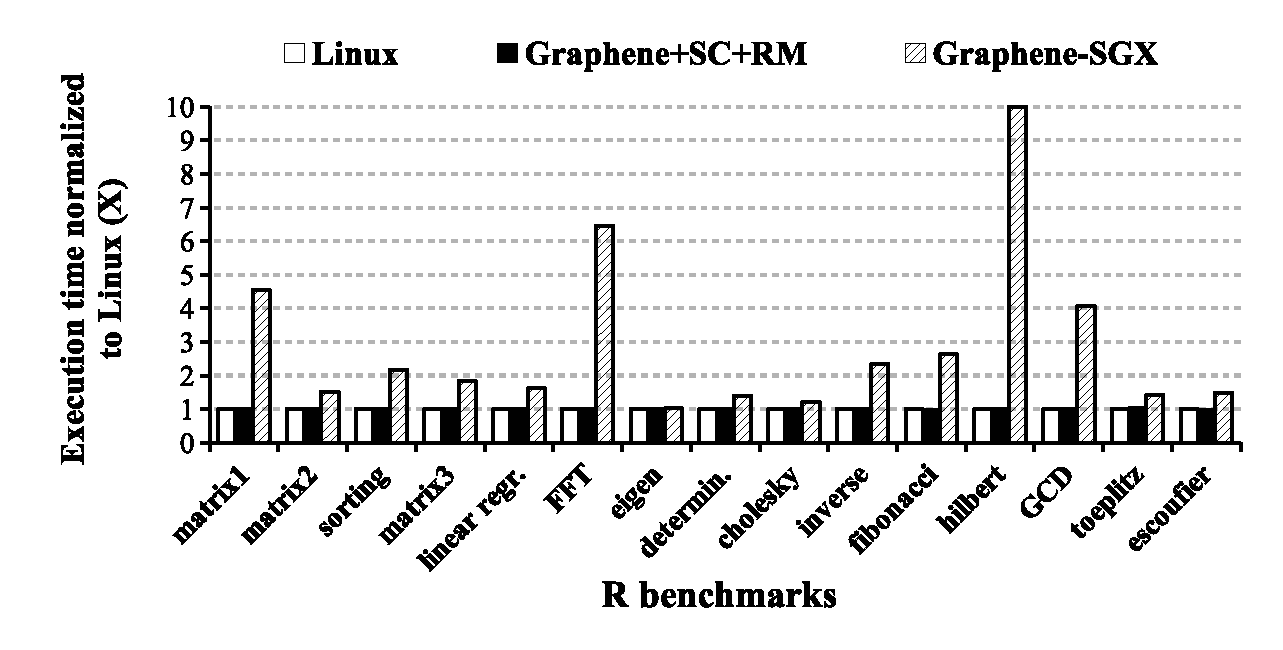
\includegraphics[width=\linewidth]{sgx/r-overhead}\\
{\bf (a) R}
\end{minipage}
\begin{minipage}{.275\textwidth}
\centering
\includegraphics[width=\linewidth]{sgx/gcc-overhead}\\
{\bf (b) GCC}
\end{minipage}
\begin{minipage}{.25\textwidth}
\centering
\includegraphics[width=\linewidth]{sgx/curl-overhead}\\
{\bf (c) CURL}
\end{minipage}

\caption{Performance overhead on desktop applications, including latency of R, execution time of GCC compilation, download time with CURL. The evaluation compares native Linux, \graphene{}, and \graphenesgx{}.} %{\bf Enclave creation time is deducted from the GCC execution time.}}
\label{fig:desktop-overhead}
\end{figure*}



\subsection{Command-Line applications}


We also evaluate the performance of a few commonly-used command-line applications.
%, to evaluate the performance of \graphenesgx{} on PCs instead of servers and clouds.
Three off-the-shelf applications are tested in our experiments:
{\bf R} (v3.2.3) for statistical computing~\cite{r-project}; {\bf GCC} (v5.4), the general GNU C compiler~\cite{gcc}; {\bf CURL} (v7.74), the default command-line web client on UNIX~\cite{curl}.
These applications are chosen because they are frequently used by Linux users,
and each of them potentially  be used 
in an enclave to handle sensitive data---either on a server or a client
machine.
% can realize profitable scenarios of using enclaves on desktop machines.



We evaluate the latency or execution time of these applications. 
%, because desktop users tend to care more about responsiveness than throughput.
In our experiments, both R and CURL have internal timing features to measure the wall time
of individual operations or executions.
%However, for other applications like GCC which does not include internal timing, evaluating the execution time can be influenced by many factors.
On a Linux host, the time to start a library OS is higher than a simple 
process, but significantly lower than booting a guest OS in a VM or
starting a container. 
Prior work measured Graphene (non-SGX) start time at 641 $\mu$s~\cite{tsai14graphene}, whereas starting an empty Linux VM takes 10.3s and starting a Linux (LXC) container takes 200 ms~\cite{agarwal15container}. 
%% dp; Note that this is MILLI seconds, not micro seconds.
%average memory footprint of an empty Linux VM, with memory deduplication, is about 96MB, . 


On SGX, the enclave creation time is relatively higher, \fixme{added more detailed number} ranging from 0.5s (a 256MB enclave) to 5s (a 2G enclave), which is a fixed cost that any application framework
will have to pay to run on SGX.
%For library OSes, the time for creating and initializing an enclave is not trivial, because it is similar to booting an lightweight OS.
% a significant part of the start-up time
% of an application is more significant, because creating enclaves is expensive.
%We consider the enclave creation time as a fixed cost for any application running in \graphenesgx{},
%and acceptable to users as long as it is responsive.
Enclave creation time is determined by the latency of the hardware and the Intel kernel driver, and is primarily a function of the size of 
the enclave, which is specified at creation time because it affects the enclave signature. %\fixmedp{although can't it grow with eadd?}.  
For non-server workloads that create multiple processes during execution,
such as GCC in Figure~\ref{fig:desktop-overhead},
the enclave creation contributes a significant portion to the execution time overheads, illustrated as a stacked bar.
%Since the enclave creation time is related to the enclave size, and unrelated to the workload,
%we deduct the enclave creation time from the execution time of GCC in Figure~\ref{fig:desktop-overhead}. \fixmedp{I think it might be better to show this as a stacked bar instead of just removing it.  Opaquely subtracting this cost doesn't seem right.  Let's discuss dp: I thought we agreed to change this...}

{\bf R}~\cite{r-project} is a scripting language often used for
data processing and statistical computation.
With enclaves, users can process sensitive data on an
OS they don't trust.
We use an R benchmark suite developed by Urbanek et al.~\cite{r-benchmark-25}, which includes 15 CPU-bound workloads such as matrix computation and number processing.
\graphenesgx{} slows down by less than 100\% on the majority of the workloads, excepts the ones which involve allocation and garbage collection: ({\tt matrix1} creates and destroys matrices, and both {\tt FFT} and {\tt hilbert} involve heavy garbage collection.)
Aside from garbage collection, these R benchmarks do not frequently interact with the host.
We further note that non-SGX \graphene{} is as efficient as Linux on all workloads, 
and these overheads appear to be SGX-specific.
%\fixmedp{Check this pontification}
In our experience, garbage collection and memory management code in managed language runtime
systems tends to be written with assumptions that do not match enclaves,
such as a large, sparse address space or that memory can be demand paged 
nearly for free (SGX version 1 requires all memory to be mapped
at creation); a useful area for future work would be to design
garbage collection strategies that are optimized for enclaves.
%we believe the overheads on \graphenesgx{} are contributed by enclaves.
 
{\bf GCC}~\cite{gcc} is a widely-used C compiler.
By supporting GCC in enclaves, developers can compile closed-source applications on customers' machines,
without leaking the source code.
GCC composes of multiple binaries, including {\tt cc1} (compiler), {\tt as} (assembler), and {\tt ld} (linker).
Therefore, GCC is a multi-process program using \syscall{execve}.
We test the compilation of thee source files with varied sizes,
using single C source files collected by MIT~\cite{gcc-benchmark}.
Each GCC execution typically \fixme{it's five, not four} creates five processes, and we run each process in a 256MB enclave by default.
%and has a fixed cost on enclave creation, which is unrelated to workload and depends on the enclave size.
%\fixme{check this}
\fixme{clarified this part, to prevent confusion between latency and overhead. also, GCC numbers got better.}
For a small workload like compiling {\tt gzip.c} (5 kLoC), running in \graphenesgx{} (4.1s) is 18.7$\times$ slower than Linux (0.2s).
The bulk of this time is spent in enclave creation, taking 3.0s in total, while the whole execution inside the enclaves, including initialization of the library OS and OS shield, takes only 1.1s, or 4.2$\times$ overhead.
For larger workloads like {\tt oggenc.c} (50 kLoC) and {\tt gcc.c} (500 kLoC), 
the overhead of \graphenesgx{} is less significant. % (3.6$\times$ and 2.1$\times$ overhead, respectively).
For {\tt gcc.c} (500 kLoC), we have to enlarge one of the enclaves ({\tt cc1}) to 2GB,
but running on \graphenesgx{} (53.1s) is only 2.1$\times$ slower than Linux (17.2s),
and 7.1s is spent on enclave creation.
%and the creation of four enclaves takes 8s.
%Each compilation has a fixed enclave creation time in \graphenesgx{}, which is about 1--2 seconds per enclave. We deduct the creation time of all enclaves  to gain more meaningful results, but do not hide rest of the overhead on fork.
%\fixmedp{Also not comfortable with this; add a bar?}
%In general, GCC in \graphenesgx{} is 1--5$\times$ slower than GCC on native Linux. 
%\fixmedp{This really needs some profiling if possible}
The overhead of non-SGX \graphene{} on GCC is marginal.
 



{\bf CURL}~\cite{curl} is a command-line  web downloader.
\graphenesgx{} can make CURL into a secure downloader that attests both server and client ends.
We evaluate the total time to download a large file, ranging from 1MB to 1GB, from another machine running Apache. % over Gigabit LAN.
%across high-speed university network\fixmedp{more specific, as above}.
\graphene{} has marginal overhead on CURL, and
\graphenesgx{} adds 7--61\% overhead to the downloading time of CURL, due to the latency of I/O.


\begin{figure*}[t!]
\centering

\begin{minipage}{.3\textwidth}
\centering
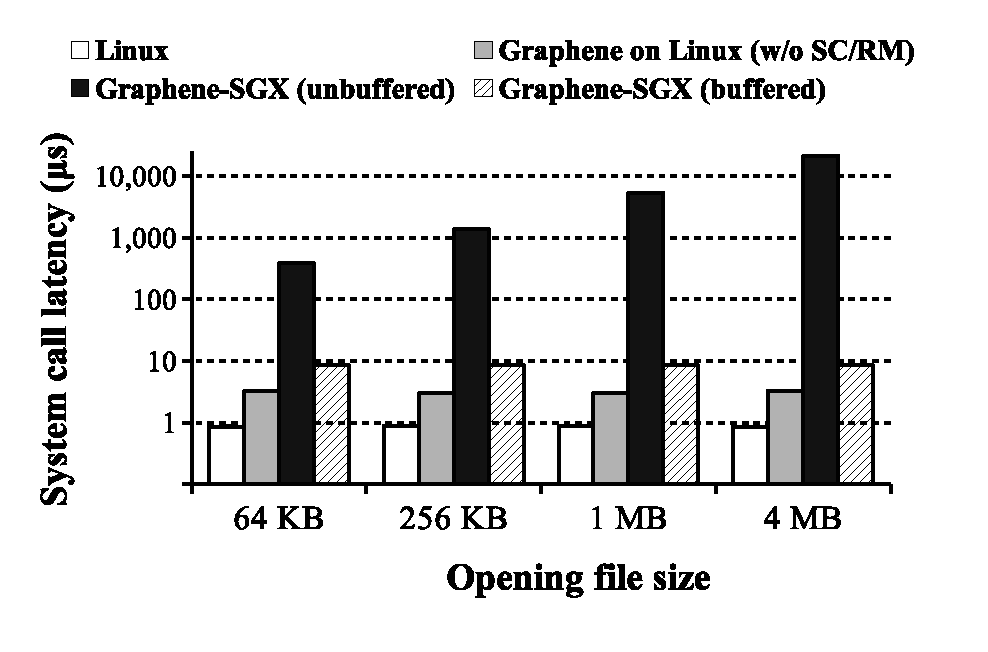
\includegraphics[width=\linewidth]{sgx/open-latency}\\
{\bf (a) Open a file}
\end{minipage}
\begin{minipage}{.3\textwidth}
\centering
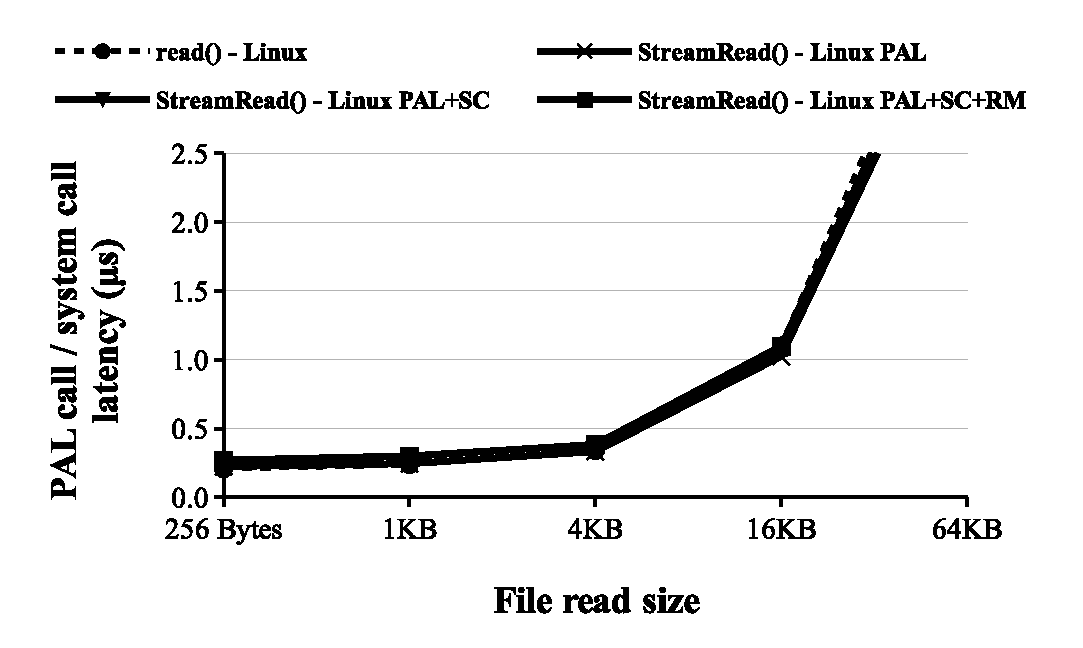
\includegraphics[width=\linewidth]{sgx/read-latency}\\
{\bf (b) Read a file}
\end{minipage}
\begin{minipage}{.3\textwidth}
\centering
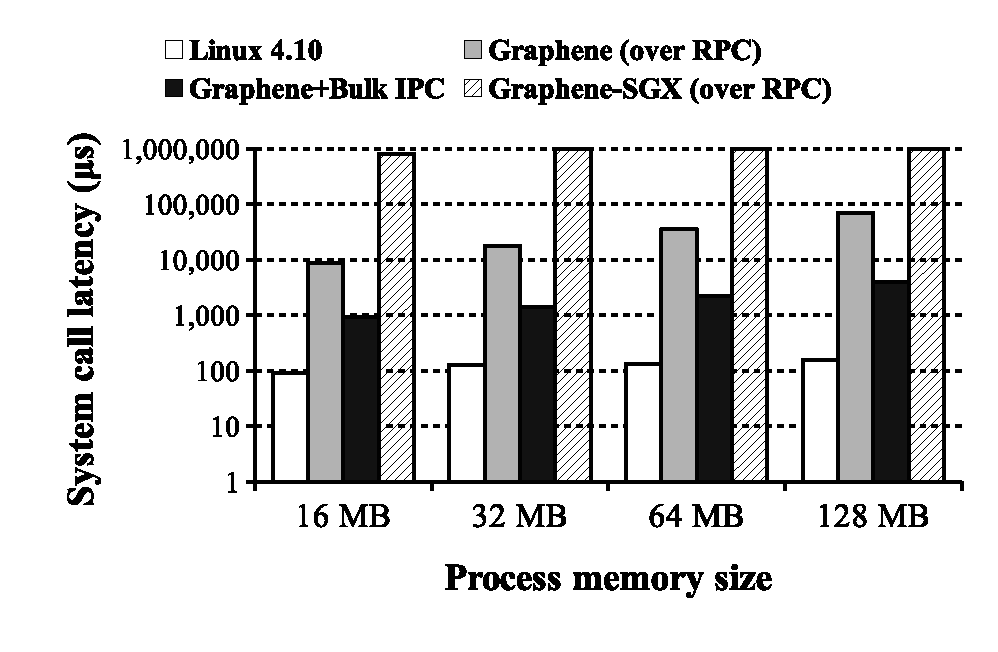
\includegraphics[width=\linewidth]{sgx/fork-latency}\\
{\bf (c) Fork a process}
\end{minipage}

\caption{Latency of some expensive system calls in \graphenesgx{}, including opening and reading a secured (authenticated) file, and forking a new process. The results are compared with native Linux and \graphene{}.}
\label{fig:syscall}
\end{figure*}


\subsection{Performance Overhead Analysis}


In this section we evaluate a few system operations that are heavily impacted by the \graphenesgx{} design.
%To shield dynamic loading and process creation,
%\graphenesgx{} uses computationally-expensive cryptographic techniques \fixmedp{more specific?} to verify enclave inputs.
% under the circumstance that the host OS cannot be trusted.
%As a trade-off to the security, the performance will be affected
%by additional cryptographic computation.
We measure the \syscall{open}, \syscall{read}, and \syscall{fork} system calls
using LMbench 2.5~\cite{McVoy:lmbench}.
A primary source of the overheads on these system calls is the cost of shielding applications, with run-time checks on the inputs.
Cryptographic techniques are used to: (1) validate the file against the secure hash, at \syscall{open}, (2) check the file chunks against the Merkle tree, at \syscall{read}, and (3) establish a TLS connection over inter-enclave RPC, at \syscall{fork}.
%opening a integrity-sensitive file for the first time, 
% or using cryptographic techniques, such as secure hashing, to verify the inputs.
% microbenchmarking specific system calls: 
% system calls,
%with different application settings.
%The microbenchmark is part of the LMBench 2.5 test suite
%\fixmedp{maybe merge this in the above paragraph, which feels a little coy}
%For instance, in order to shield dynamic loading, \graphenesgx{} checks each binary file against the secure hashes in the manifest,
%when the file is opened for the first time---after the whole file is copied into the enclave.
%\fixmedp{This happens after they are copied into enclave, memory right?}
%The verification happens when opening the file for the first time (often by the 
%After \graphenesgx{} validates the file, we generate a series of hashes of the file in chunks, as a merkle tree.
%to prevent verifying the whole file again when later randomly reading a part of the file.
%\fixmedp{So is this for the case when a file is swapped out?  I'm confused here - some details are missing}
%The latency of opening and reading an authenticated file in \graphenesgx{} is dominated by SHA256 and SHA512 calculation.
The remaining overheads contribute to exiting the enclave for host system calls, and bringing memory into the EPC (enclave page cache) or decrypting 
memory on a last-level cache miss. %and later the cache where the memory is decrypted by the CPU.


Figure~\ref{fig:syscall}(a)
shows the overhead for authenticating files in \syscall{open}.
\fixme{change overhead to latency}
Depending on the file size, the latency of \syscall{open} on \graphenesgx{} is 383$\mu$s (64KB file) to 21ms (4MB file), whereas on Linux, the latency is constant at 0.85$\mu$s.
We note that this is where enclaves are at a disadvantage, as \syscall{open} 
normally does not need to read file content; whereas here \graphenesgx{} uses \syscall{open}
as a point at which to validate file content.
For a subsequent \syscall{open}, when the Merkle tree is already generated, the overhead of simply exiting enclave for \syscall{open}, and searching the file list in the manifest, is about 9$\times$.
%\fixmedp{why?}


One might be able to optimize further for cases where only part of a file is accessed
with incremental hashing.  However, in the common case where nearly all of the file is accessed,
these costs are difficult to avoid when host file system is untrusted.
Another opportunity 
is to create the Merkle tree offline, when the manifest is created.
%\fixmedp{I think the second idea has legs...}


%This is an inevitable cost, because normal \funcname{open} on trusted OSes
%need not to access file content.
%After verifying the file, \graphenesgx{} buffers the chunk hash values, to skip whole-file verification when the file is reopened.

Figure~\ref{fig:syscall}(b)
shows the overhead for authenticating files in \syscall{read}, which 
is lower than \syscall{open}.
Since the whole file has been verified at \syscall{open}, the sequential \syscall{read} only verifies the chunks of files it is reading from untrusted memory.
%Reads from data cached in enclave memory are cheaper.  %\fixmedp{right? can we say how much cheaper?  Maybe add separate bars for both cases?}
% Therefore, \syscall{read} is actually much cheaper than \syscall{open}.
Depending on the size of blocks being read, the latency on \graphenesgx{} is 0.5$\mu$s (64-byte \syscall{read}) to 16.9$\mu$s (4KB \syscall{read}). The latency of \syscall{read} on Linux is \roughly{}0.1$\mu$s for any block size below 4KB.
If the file is not authenticated,
\graphenesgx{} only copies the file contents into the buffer, and the overhead reduces to 48\% (64-byte \syscall{read}) to 83\% (4KB \syscall{read}).
\fixmedp{Consider doing larger buffers, say up to 64k or even 4 MB}

%\fixmedp{In the legend for 7b, unsecure should be insecure}


Figure~\ref{fig:syscall}(c) shows the overhead of forking a process.
As described in \ref{sec:multiproc}, the latency of \syscall{fork} in \graphenesgx{} is affected by three factors:
creation of a new enclave, local attestation of the integrity, and duplicating the process state over an encrypted RPC stream.
Combining these factors, \syscall{fork} is one of the most expensive calls in \graphenesgx{}.
%, but at least it is supported natively on the current hardware.
The default enclave size is 256MB.
%which takes \roughly{}0.5s to create. 
Our evaluation shows that the latency of forking a process is around 0.8s (16MB process) to 2.7s (128MB process), but can be more expensive if the parent process uses more memory.
The trend matches the performance of \graphene{} without the bulk IPC optimization.
\fixmedp{If you want, some thoughts on how this might be improved in the future would be nice...  One good suggestion is recycling enclaves, or pre-forking so measurements can be done in parallel}
%Due to the overhead on \funcname{fork}, \graphenesgx{} is not suitable for fork-intensive workloads like Bash scripts
%if performance is critical.

\fixme{talk about a limitation of improving fork. check this.}
One way to further optimize \syscall{fork} is to reduce or avoid enclave creation time; one can potentially pre-launch a child enclave, and then migrate the process contents later when \syscall{fork} is called.
There might be another opportunity to improve the latency of process migration,
if copy-on-write sharing of enclave pages can be supported in future generations of SGX.
%Unfortunately, sending the process contents is difficult to avoid in \syscall{fork},
%as SGX disallows sharing enclave memory between multiple enclaves.

%\fixmedp{I assume 5.4 isn't done yet}



\subsection{TCB Size and Shielded Functionality}

In this section we measure the increase in TCB size of \graphenesgx{},
%in lines of code, 
as well as 
%compare the TCB size increased by \graphenesgx{} to an unmodified application, in lines of code, and 
the OS functionality shielded by the framework.
We compare to \scone{} and \panoply{}, using
%For SCONE and Panoply, we use 
numbers reported in their papers. 
%The conventional One generally assumes 
A smaller TCB is generally easier to review or possibly verify,
and is assumed to have fewer vulnerabilities.
%more implies lower burden for code review or formal verification, and less risk of writing exploitable code.
%For instance, Panoply argues that, because its use cases are typically smaller than 20kLoC, including both the application logic and Panoply itself, it is within the realm of future, automated verification~\cite{shinde17panoply}.

\fixmedp{Reviewer B asks for memory footprint, which isn't a bad idea}

\begin{table}
\footnotesize
\centering
\bgroup
\def\arraystretch{1.2}
\setlength{\tabcolsep}{0.5em}
\begin{tabular}{>{\raggedright\arraybackslash}p{9em}>{\raggedleft\arraybackslash\bf}p{7em}>{\raggedleft\arraybackslash}p{4.25em}>{\raggedleft\arraybackslash}p{4.25em}}
Components                    & \graphenesgx{}  & \scone{}     & \panoply{}  \\
\hline
libc (ld, libm, pthread)      &  1,292 &   88 & --      \\
                              & (glibc-2.19) & (musl)   &          \\
Library OS                    &     34 &  --      & --     \\
PAL / OS Shield               &     22 &   99 & 10  \\
\hline
Total                         &  1,348 &  187 & 10  \\
\hline
\end{tabular}
\egroup
\caption{TCB size (in thousands of lines of code) of \graphenesgx{}, \scone{}, and \panoply{}.}
\label{tab:tcb-size}
\end{table}

Table~\ref{tab:tcb-size} lists the lines of code in each components within the TCB of \graphenesgx{}, \scone{}, and \panoply{}.
By comparing the total TCB size, \graphenesgx{} is 9$\times{}$ larger than \scone{}, and 134$\times{}$ larger than \panoply{}.
However, the primary difference is the selection of libc: 
for maximum compatibility, \graphene{} uses glibc.
\scone{} uses the smaller musl libc, which lacks some features of glibc.
%it would be easy to use the smaller, and incomplete, musl libc.
%SCONE uses 
% Linux applications, \graphenesgx{} chooses to use a minimally-modified glibc, whereas SCONE uses the much more lightweight musl and 
\panoply{} excludes libc from its TCB,
% \fixmedp{what is their rationale, again? Check this}
to fit into the range of automated formal verification,
as they shield at the libc interface.
In principle, \graphene{} could easily support musl as well as glibc for applications
that do not need the additional features of glibc.
We also see the benefit of removing unused code from 
libraries, especially in an unsafe language,
similar to the approach taken in unikernels~\cite{unikernels}.
On balance, 
this choice of libc implementation is largely orthogonal to the issue
of how general-purpose the shields are.

%We argue that the choice of libc is orthogonal to the design of \graphenesgx{}; one can statically compile the applications against musl or glibc if TCB size is a concern, or given plenty of time, trim the libc functionality to bare minimum. 

If we focus on the TCB size of the library OS and the shields, 
\graphenesgx{} is 
%library OS and PAL in \graphenesgx{}, with the shielding layer of SCONE, we are 
44\% smaller than \scone{}. 
We cannot analyze the size of \scone{} because it is closed source.
%, although
%we suspect
%Although it is unclear what is in the implementation of SCONE, because it is not yet open-sourced, we believe the largest portion of their TCB contributes to the cryptography library.
\panoply{} has a smaller TCB in its shield, but within the same order of magnitude.
Panoply only shields 91 out of 256 supported POSIX functions; for context, POSIX 1003.1 defines 1,191 APIs~\cite{POSIX1003-1-2008}.
%out of 256 currently supported by \panoply{} \fixmedp{The better number is how many total functions in POSIX}.

All three of these compatibility layers or shields are within the same
order of magnitude in code size, and the differences are likely 
correlated with different ranges of supported functionality.
A recent study indicates that only order-of-magnitude differences in code
size correlate with reported CVE vulnerabilities; within the same order-of-magnitude,
the data is inconclusive that there is a meaningful difference in risk~\cite{security-metric}.
Thus, increased generality does not necessarily come with 
increased risk. % is not a clear relationship between risk 

% data only correlates
%with differences in code size when 

%Besides the choice of libc, we argue that the TCB size of a library OS or a shim shielding layer is actually correlated with the functionality that it supports or shields. Because none of the three frameworks have completely shielded the whole Linux system call table or POSIX, it is unclear how much code has to be added in the future. \graphenesgx{} also shows that one can always engineer a library OS with a small TCB, if most code is not reused from a monolithic OS kernel like Windows or Linux.
%A recent study of the CVE database also points out that having a larger TCB does not necessarily indicate more vulnerabilities, even when the difference is more than two order-of-magnitude. 



\input{apistudy}

\makeatletter
\def\input@path{{}}
\makeatother
\graphicspath{{}}
\section{Conclusion}

This paper demonstrates that the costs of running an unmodified application in SGX on a library OS are
marginal compared to thinner shims.
The major costs of using SGX are still hardware limitations of SGX.
As SGX and similar technologies mature, these design choices may have more impact.
In the interim, \sysname{} serves as a simple, open-source tool to quickly bring up
existing applications on SGX, and then incrementally adapt the code to improve performance and security on SGX.
%\fixme{Mona suggests dropping this}
%We believe the \sysname{} design is sufficiently general that porting applications to AMD's PSP
%features should only require porting the PAL.
%\fixme{Mona suggest adding this argument:
%``Graphene-SGX can provide support for running unmodified applications on SGX that provide encryption and integrity Vs SEV that can run unmodified applications, but provides only encryption but no integrity guarantees.''}


\newpage
\begin{appendices}
\chapter{Formal Definitions of \UsageMetric{} and \CompatMetric{}}
\label{chap:defs}

%\fixmedp{The formal definition of importance in section 2.1 is hard to follow, in part because of the naming. The names of variables (Dependentapi, inst) don't make clear the types of the variables (a package, set of packages, set of API, instance, set of instance) etc. It would be helpful to reconsider the terminology to make the variable types more clear.
%In the equations in 2.2, explaining what E means would be helpful, as it is not obvious from the context. Also, should Weighted Compliance be a function of the instance in addition to the API?
%}

\section{\UsageMetric{} --- A Metric for APIs}
\label{sec:defs:usagemetric}

\vspace{0.1in}
{\noindent
\fbox{\begin{minipage}{\linewidth}
\setlength{\parindent}{-0.1in}
\setlength{\leftskip}{0.1in}
\setlength{\rightskip}{0.1in}
 Definition: {\bf \UsageMetric{}.} \\
For a given API, the probability that an installation includes
at least one application requiring the given API.
%at least one broken application
%(whose API footprint covers the target API),
%if the target API was removed.
\end{minipage}}}
\vspace{0.1in}

A system installation ($\mathtt{inst}$)
is a set of packages installed ($\{\mathtt{pkg}_1, \mathtt{pkg}_2, ..., \mathtt{pkg}_k \in \mathtt{Pkg}_\mathtt{all}\}$).
For each package ($\mathtt{pkg}$)  that can be installed by the installer,
we analyze every executable included in the package 
($\mathtt{pkg} = \{\mathtt{exe}_1, \mathtt{exe}_2, ..., \mathtt{exe}_j\}$), and
generate the API footprint of the package as:
\begin{align*}
{\mathtt{Footprint}}_{\mathtt{pkg}} = \{\mathtt{api} \in {\mathtt{API}}_{\mathtt{all}} \mid \text{\parbox{2.3in}{$\exists \mathtt{exe} \in \mathtt{pkg}$,
$\mathtt{exe}$ has usage of $\mathtt{api}$}}\}
\end{align*}

\noindent
For a target API, \usagemetric{} is calculated as the probability
that any installation includes
at least one package that uses the API;
i.e.,
the API belongs to the footprint of at least one package.
Using \osdist{}'s package installation statistics, one can calculate the
probability that a specific package is installed as:
\begin{align*}
Pr\{\mathtt{pkg} \in \mathtt{Inst}\} = \frac{\text{\# of installations including $\mathtt{pkg}$}}{\text{total \# of installations}}
\end{align*}

\noindent
Assuming the packages that use an API are  
$\mathtt{Dependents}_\mathtt{api} = \{\mathtt{pkg}|\mathtt{api} \in \mathtt{Footprint}_\mathtt{pkg}\}$.
\Usagemetric{} is the probability that at least one package
from $\mathtt{Dependents}_\mathtt{api}$ is installed on a random installation, which is calculated as follows:
\begin{align*}
&\mathtt{Importance}(\mathtt{api}) = Pr\{\mathtt{Dependent}_\mathtt{api} \bigcap \mathtt{Inst} \neq \emptyset\} \\
&= 1 - Pr\{\forall \mathtt{pkg} \in \mathtt{Dependent}_\mathtt{api}, \mathtt{pkg} \notin \mathtt{Inst}\} \\
&= 1 - \prod_{\mathtt{pkg} \in \mathtt{Dependent}_\mathtt{api}} Pr\{\mathtt{pkg} \notin \mathtt{Inst}\} \\
&= 1 - \prod_{\mathtt{pkg} \in \mathtt{Dependent}_\mathtt{api}} (1 - \frac{\text{\# of installations including $\mathtt{pkg}$}}{\text{total \# of installations}})
\end{align*}

\section{\CompatMetric{} --- A System-Wide Metric}
\label{sec:defs:compatmetric}

%% An accurate metric for API compatibility must take into account at least two factors:
%% \begin{compactenum}
%% \item For each interface in the API, what are the applications that rely on it and could be affected if the interface is removed? ({\em application footprint})
%% \item For each application, how many installations of the system in the world has included it? ({\em application popularity})
%% \end{compactenum}


%% \fixmedp{Term for each call, vs system overall: API Importance and Effective Coverage?}

%% To accurately evaluate compatibility, we design a metric that is quantifiable, \fixmetsai{one more word here}, and easy to interpret.

\begin{comment}
We defined {\bf platform compatibility} as "{\em the probability of porting any installation of an OS distribution onto the target OS without any effort}".
The definition of an {\em installation} is a combination of application setup on a standalone OS instance.
An Installation can exist on physical machines,
or any machines of generalized sense such as a virtual machines, containers or subsystems.
In our model, installations represent customers of the OS, who are considered equal when providing any services.
\end{comment}

\vspace{0.1in}
%\fixmetsai{Find a good name for our metric} 
{\noindent
\fbox{\begin{minipage}{\linewidth}
\setlength{\parindent}{-0.1in}
\setlength{\leftskip}{0.1in}
\setlength{\rightskip}{0.1in}
Definition: {\bf \CompatMetric{}.} \\
For a target system, the fraction of applications supported,
weighted by the popularity of these applications.
\end{minipage}}}
\vspace{0.1in}

\Compatmetric{} is used to evaluate the relative compatibility on a system that
supports a set of APIs ($\mathtt{API}_\mathtt{Supported}$).
For a package on the system, we define it as supported if 
if every API that the package uses is in the supported API set.
In other words, a package is supported if it is a member of the following set:
\begin{align*}
\mathtt{Pkg}_\mathtt{Supported} = \{\mathtt{pkg} | \mathtt{Footprint}_\mathtt{pkg} \subseteq \mathtt{API}_\mathtt{Supported}\}
\end{align*}

\noindent
Using \compatmetric{}, one can estimate the fraction of packages in an installation that end-users can expect a target system to support.
For any installation
that is an arbitrary subset of available packages
($\mathtt{Inst} = \{\mathtt{pkg}_1, \mathtt{pkg}_2, ..., \mathtt{pkg}_k\} \subseteq \mathtt{Pkg}_\mathtt{all}$),
\compatmetric{} is the expected value of
the fraction in any installation ($\mathtt{Inst}$)
that overlaps with the supported packages ($\mathtt{Pkg}_\mathtt{Supported}$):
\begin{align*}
\mathtt{Weighted Completeness}(\mathtt{API}_\mathtt{Supported}) =
E(\frac{|\mathtt{Pkg}_\mathtt{Supported} \bigcap \mathtt{Inst}|}{|\mathtt{Inst}|}) 
\end{align*}
where $E(\mathtt{X})$ is the expected value of $\mathtt{X}$.

Because we do not know which packages are installed together,
except in the presence of explicit dependencies,
%Lacking of the distribution data of each package, we approximate the value of \compatmetric{}
%by ignoring {\em higher order} estimators
%of the expectation, assuming events of installing each package to be independent.
we assume package installation events are independent.
Thus, the approximated value of \compatmetric{} is:
\begin{align*}
\frac{E(|\mathtt{Pkg}_\mathtt{Supported} \bigcap \mathtt{Inst}|)}{E(|\mathtt{Inst}|)}
\sim \dfrac{\sum_{\mathtt{pkg} \in \mathtt{Pkg}_\mathtt{Supported}} (\dfrac{\text{\# of installations including $\mathtt{pkg}$}}{\text{total \# of installations}})}{\sum_{\mathtt{pkg} \in \mathtt{Pkg}_\mathtt{all\hspace{0.21in}}} (\dfrac{\text{\# of installations including $\mathtt{pkg}$}}{\text{total \# of installations}})}
\end{align*}

\end{appendices}

\newpage
\phantomsection
\addcontentsline{toc}{chapter}{References}
\renewcommand{\bibname}{\centerline{\normalsize\bf{References}}}
\bibliographystyle{plainnat}
\bibliography{bibliography}



\end{document}
